\documentclass[11pt]{article}
\usepackage[utf8]{inputenc}

% --- PACKAGES ---
\usepackage{amsmath}
\usepackage{geometry}
\usepackage{graphicx}
\usepackage{longtable}
\usepackage{booktabs}
\usepackage[T1]{fontenc}
\usepackage{listings}
\usepackage{subcaption} % For arranging plots with sub-captions
\usepackage{braket}
\usepackage{placeins}
\usepackage{caption}
\usepackage{float}
\usepackage{amssymb}
\usepackage{authblk}
\usepackage{xcolor} % For code listing colors

% --- HYPERREF (LOAD TOWARDS THE END) ---
% This ensures it can correctly handle links for elements from other packages.
\usepackage{hyperref} 


% --- DOCUMENT SETUP ---
\geometry{a4paper, margin=1in}

% Setup for hyperlinks: urlcolor is for external links, linkcolor for internal (ToC, refs)
\hypersetup{colorlinks=true, urlcolor=blue, linkcolor=black}

% Setup for code listings
\definecolor{codegreen}{rgb}{0,0.6,0}
\definecolor{codegray}{rgb}{0.5,0.5,0.5}
\definecolor{codepurple}{rgb}{0.58,0,0.82}
\definecolor{backcolour}{rgb}{0.95,0.95,0.92}

\lstdefinestyle{mystyle}{
    backgroundcolor=\color{backcolour},
    commentstyle=\color{codegreen},
    keywordstyle=\color{magenta},
    numberstyle=\tiny\color{codegray},
    stringstyle=\color{codepurple},
    basicstyle=\ttfamily\footnotesize,
    breakatwhitespace=false,
    breaklines=true,
    captionpos=b,
    keepspaces=true,
    numbers=left,
    numbersep=5pt,
    showspaces=false,
    showstringspaces=false,
    showtabs=false,
    tabsize=2
}
\lstset{style=mystyle}


% --- DOCUMENT START ---
\begin{document}
\title{Determination of reconstruction efficiency}
\author[1]{Chatura Kuruppu}
\affil[1]{New Mexico State University, Las Cruces, NM 88003}
\date{\today}
\maketitle

\begin{abstract}
\noindent This document outlines the methodology for determining the dimuon reconstruction efficiency required for the Drell-Yan double-differential cross-section measurement. Efficiency correction factors are derived using Monte Carlo simulations and applied to experimental data. The efficiency $\epsilon$ is parameterized as a function of the kinematic variables, Feynman-x ($x_F$) and dimuon invariant mass ($m$). We detail the procedure for calculating the average efficiency $\langle\epsilon\rangle$ for each kinematic bin by applying a linear interpolation method to data events. The propagation of statistical uncertainties is rigorously derived, and the final correction factors, $1/\langle\epsilon\rangle$, are presented for different datasets and target configurations.
\end{abstract}
\clearpage

\tableofcontents
\clearpage

\listoffigures
\clearpage

\listoftables
\clearpage


% --- METHODOLOGY PART 1 ---
\section{Introduction}
We report DY absolute double differntial cross-section for different Mass and $x_{F}$ bins. It is necessary to correct the reconstruction efficiency for different $x_{F}$ and Mass bins using Monte-Carlo events. In this study we first generate efficiency curves for different Mass and $x_{F}$ bins and then calculate average efficiency $<\epsilon>$ using the methodology developped by Harsha and iterating through data (RS67, RS57-70) for each 2-dimensional bin range. Then the correction factor: $1/<\epsilon>$ will be applied when calculating cross-section.

\subsection{Dimuon Events Used}
Following files were used to calculate kTracker efficiency for different Mass and $x_{F}$ bins:
\begin{itemize}
 \item Following Monte-Carlo files were used to generate efficiency curves for different Mass and $x_{F}$ bins:
 \begin{itemize}
  \item mc\_drellyan\_LH2\_M027\_S002\_messy\_occ\_pTxFweight\_v2.root
  \item mc\_drellyan\_LH2\_M027\_S002\_clean\_occ\_pTxFweight\_v2.root
 \end{itemize}
 \item Following data files were used to calculate average efficiency for different Mass and $x_{F}$ bins:
 \begin{itemize}
	 \item R008\_roadset67\_0\_2111v42\_tmp\_noPhys\_noOcc.parquet
  \item roadset57\_70\_R008\_2111v42\_tmp\_noPhys.parquet
 \end{itemize}
\end{itemize}


The reconstruction efficiency curves were generated for different Mass and $x_{F}$ bins by taking the ratio: 
$$Efficiency\ (\epsilon) = \frac{Number\ of\ messy\ dimuon\ events}{Number\ of\ clean\ dimuon\ events}$$ 
that passes all event selection cuts. This is calculated as a function of the D2 variable, binned in Feynman-x ($x_F$) and dimuon mass ($m$).

\subsection{Bin ranges}
This efficiency study is conducted by using the same bin ranges defined in Shivangi's cross-section script.
Following bins widths are defined to calculate efficiency corrections.
\begin{itemize}
 \item $x_{F}$ bins: [0.0, 0.05, 0.1, 0.15, 0.2, 0.25, 0.3, 0.35, 0.4, 0.45, 0.5, 0.55, 0.6, 0.65, 0.7, 0.75, 0.8, 0.85]
 \item Mass bins: [4.2, 4.5, 4.8, 5.1, 5.4, 5.7, 6.0, 6.3, 6.6, 6.9, 7.5, 8.7]

\end{itemize}

\subsection{Event Selection}
Following event selection criteria applied to Monte-Carlo events mentioned in section. I am using the same event selection criteria defined by Hugo's analysis.
\begin{itemize}
 \item Event selection applied to messy events:
  \begin{itemize}
   \item Base cuts: chuckCutsPositive\_2111v42\_tmp \&\& chuckCutsNegative\_2111v42\_tmp \&\& chuckCutsDimuon\_2111v42 \&\& physicsCuts\_noMassCut\_2111v42\_tmp \&\& occCuts\_2111v42 \&\& DYCut\_MC
   \item xF cut
   \item mass cut
  \end{itemize}
 \item Event selection applied to clean events:
  \begin{itemize}
   \item Base cuts: chuckCutsPositive\_2111v42\_tmp \&\& chuckCutsNegative\_2111v42\_tmp \&\& chuckCutsDimuon\_2111v42 \&\& physicsCuts\_noMassCut\_2111v42\_tmp \&\& DYCut\_MC
   \item xF cut
   \item mass cut
  \end{itemize}

\end{itemize}

\subsection{Determination of Efficiency for a Dimuon Event}
In order to determine efficiency for each dimuon event in data, I use the same methodology developped by Harsha.

\begin{figure}[h!]
    \centering
    % Image generation prompt: A conceptual diagram illustrating the propagation of error.
    % It should show a function (e.g., a curve) with input variables having small uncertainties (represented as error bars or shaded regions),
    % and the output variable showing a larger, propagated uncertainty.
    % Use abstract, scientific visualization style with clear labels for inputs (epsilon_+, epsilon_-) and output (epsilon).
    % The background should be clean and white, with the diagram elements in blue, green, and red to differentiate.
    % Include axes representing a multi-dimensional space.
    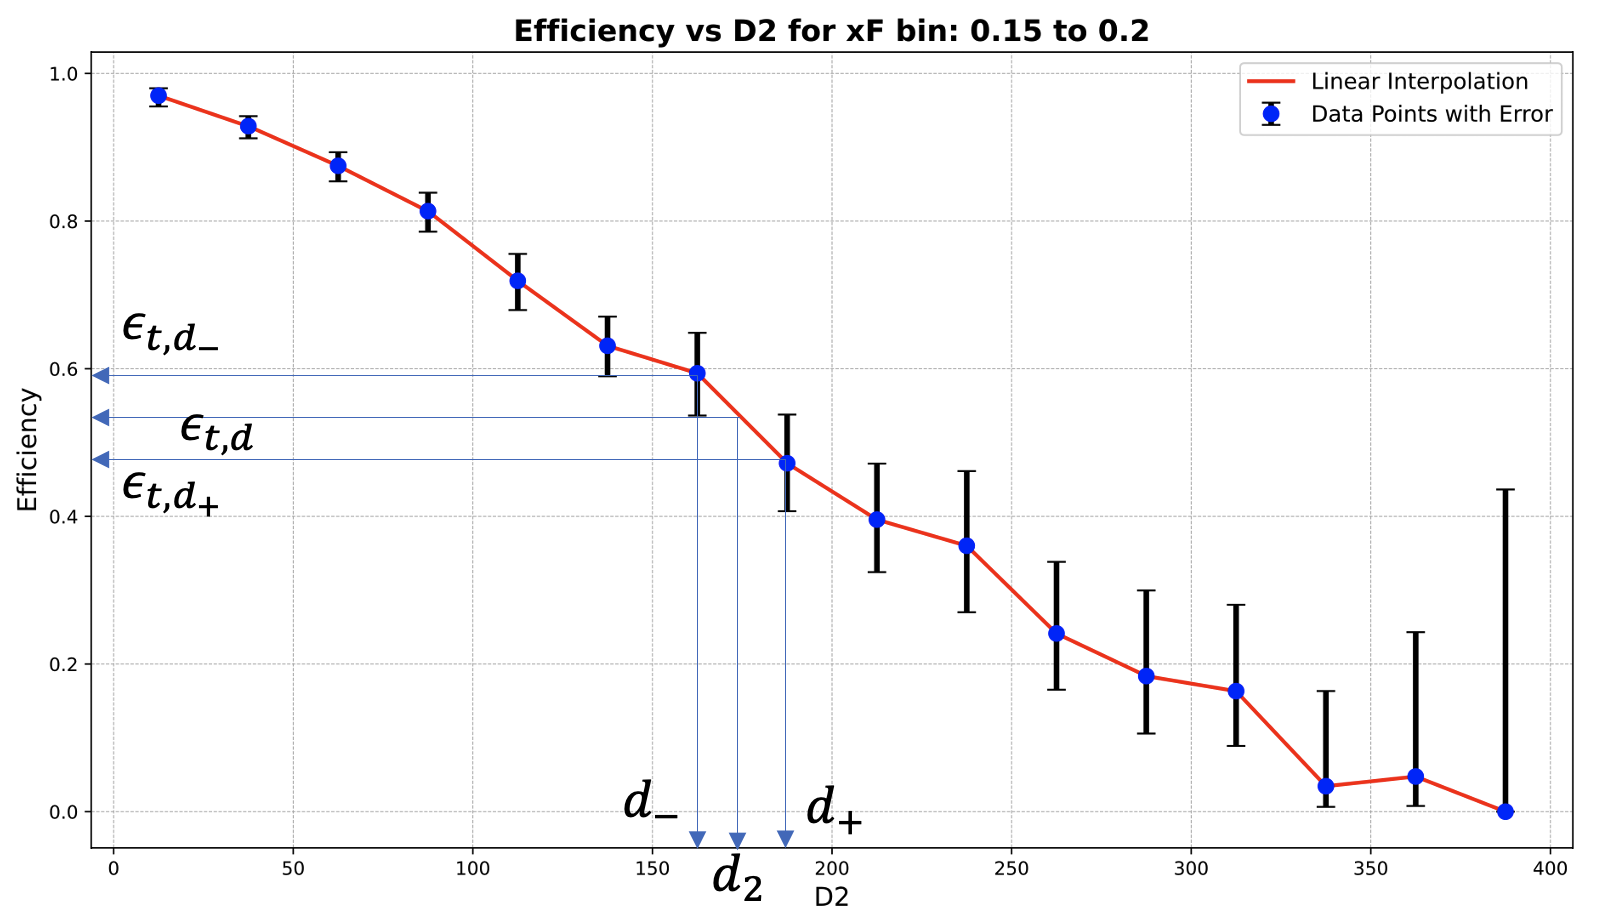
\includegraphics[width=0.8\textwidth]{error.png} % This will be replaced by the generated image
    \caption{Determination of Efficiency and it's uncertainty}
    \label{fig:error_propagation_concept}
\end{figure}


The given formula for the efficiency, denoted by $\epsilon_{t,d_{2}}$, is a function of $\epsilon_{t,d_{+}}$, $\epsilon_{t,d_{-}}$, $d_+$, $d_-$, and $d_2$:
$$
\epsilon_{t,d_{2}} = \epsilon_{t,d_{-}} - \frac{\epsilon_{t,d_{+}} - \epsilon_{t,d_{-}}}{d_+ - d_-} (d_2 - d_-)
$$
Our goal is to find the uncertainty of $\epsilon_{t,d_{2}}$, denoted as $\delta\epsilon_{t,d_{2}}$, assuming we know the uncertainties $\delta\epsilon_{t,d_{+}}$ and $\delta\epsilon_{t,d_{-}}$. The terms $d_2$, $d_+$, and $d_-$ are treated as constants with no associated uncertainty.

%\hrulefill
% --- Section 2: Error Propagation Method ---
\subsubsection{Error Propagation Method}

For a function of multiple variables, such as $\epsilon_{t,d_{2}}(\epsilon_{t,d_{+}}, \epsilon_{t,d_{-}})$, the general formula to propagate uncertainty (assuming the variables are uncorrelated) is:
$$
(\delta\epsilon_{t,d_{2}})^2 = \left(\frac{\partial \epsilon_{t,d_{2}}}{\partial \epsilon_{t,d_{+}}}\right)^2 (\delta\epsilon_{t,d_{+}})^2 + \left(\frac{\partial \epsilon_{t,d_{2}}}{\partial \epsilon_{t,d_{-}}}\right)^2 (\delta\epsilon_{t,d_{-}})^2
$$

%\hrulefill
\clearpage
% --- Section 3: Step-by-Step Derivation ---

\subsubsection{Step-by-Step Derivation}

To find the final uncertainty, we follow three main steps.

\subsubsection{Simplify the Expression for $\epsilon_{t,d_{2}}$}

To make the calculation of derivatives more straightforward, we first rearrange the formula for $\epsilon_{t,d_{2}}$:
$$
\epsilon_{t,d_{2}} = \epsilon_{t,d_{-}} - \left(\frac{d_2 - d_-}{d_+ - d_-}\right)\epsilon_{t,d_{+}} + \left(\frac{d_2 - d_-}{d_+ - d_-}\right)\epsilon_{t,d_{-}}
$$
Combining the terms that contain $\epsilon_{t,d_{-}}$, we get:
$$
\epsilon_{t,d_{2}} = \left(1 + \frac{d_2 - d_-}{d_+ - d_-}\right)\epsilon_{t,d_{-}} - \left(\frac{d_2 - d_-}{d_+ - d_-}\right)\epsilon_{t,d_{+}}
$$
We can find a common denominator for the term multiplying $\epsilon_{t,d_{-}}$:
$$
\epsilon_{t,d_{2}} = \left(\frac{d_+ - d_- + d_2 - d_-}{d_+ - d_-}\right)\epsilon_{t,d_{-}} - \left(\frac{d_2 - d_-}{d_+ - d_-}\right)\epsilon_{t,d_{+}}
$$
This simplifies to:
$$
\epsilon_{t,d_{2}} = \left(\frac{d_+ + d_2 - 2d_-}{d_+ - d_-}\right)\epsilon_{t,d_{-}} - \left(\frac{d_2 - d_-}{d_+ - d_-}\right)\epsilon_{t,d_{+}}
$$

\subsubsection{Calculate the Partial Derivatives}

With the simplified expression, we can now find the partial derivatives of $\epsilon_{t,d_{2}}$ with respect to $\epsilon_{t,d_{+}}$ and $\epsilon_{t,d_{-}}$.

\paragraph{Derivative with respect to $\epsilon_{t,d_{+}}$:}
$$
\frac{\partial \epsilon_{t,d_{2}}}{\partial \epsilon_{t,d_{+}}} = -\frac{d_2 - d_-}{d_+ - d_-} = \frac{d_- - d_2}{d_+ - d_-}
$$

\paragraph{Derivative with respect to $\epsilon_{t,d_{-}}$:}
$$
\frac{\partial \epsilon_{t,d_{2}}}{\partial \epsilon_{t,d_{-}}} = \frac{d_+ + d_2 - 2d_-}{d_+ - d_-}
$$

\subsubsection{Uncertainty Formula for one di-muon event}

Finally, we substitute these partial derivatives back into the error propagation formula:
$$
(\delta\epsilon_{t,d_{2}})^2 = \left(\frac{d_- - d_2}{d_+ - d_-}\right)^2 (\delta\epsilon_{t,d_{+}})^2 + \left(\frac{d_+ + d_2 - 2d_-}{d_+ - d_-}\right)^2 (\delta\epsilon_{t,d_{-}})^2
$$
Taking the square root of both sides gives the final expression for the uncertainty, $\delta\epsilon_{t,d_{2}}$:
$$
\delta\epsilon_{t,d_{2}} = \sqrt{\left(\frac{d_- - d_2}{d_+ - d_-}\right)^2 (\delta\epsilon_{t,d_{+}})^2 + \left(\frac{d_+ + d_2 - 2d_-}{d_+ - d_-}\right)^2 (\delta\epsilon_{t,d_{-}})^2}
$$
This can also be written in a more compact form by factoring out the denominator:
$$
\delta\epsilon_{t,d_{2}} = \frac{1}{|d_+ - d_-|} \sqrt{(d_- - d_2)^2 (\delta\epsilon_{t,d_{+}})^2 + (d_+ + d_2 - 2d_-)^2 (\delta\epsilon_{t,d_{-}})^2}
$$
\clearpage

\subsection{Average efficiency and final uncertainty}
We determine average efficiency by iterating through all the di-muon events. The final efficiency $\bar{\epsilon}$
If you have N dimuon events, each with a calculated efficiency ($\epsilon_1, \epsilon_2, \dots, \epsilon_N$) and a corresponding error ($\delta\epsilon_1, \delta\epsilon_2, \dots, \delta\epsilon_N$), you first calculate the \textbf{average efficiency}, $\bar{\epsilon}$:
$$
\bar{\epsilon} = \frac{1}{N} \sum_{i=1}^{N} \epsilon_i
$$
The \textbf{error on this average efficiency}, which we'll call $\delta\bar{\epsilon}$, is then given by the standard formula for propagation of error for a sum:
$$
\delta\bar{\epsilon} = \frac{1}{N} \sqrt{\sum_{i=1}^{N} (\delta\epsilon_i)^2}
$$
This is equivalent to writing the sum of squares explicitly:
$$
\delta\bar{\epsilon} = \sqrt{\frac{(\delta\epsilon_1)^2 + (\delta\epsilon_2)^2 + \dots + (\delta\epsilon_N)^2}{N^2}}
$$

\section{Results}
Here, we report efficiency corrections under 2 scenerios.

\begin{itemize}
	\item Efficiency calculation only by using $x_{F}$ bins (1-D Study)
	\item Efficiency calculation only by using both $x_{F}$ and Mass bins (2-D Study)
\end{itemize}



%\subsection{Generating Efficiency Curves (PDF Plots)}
%The efficiency curves are generated using a ROOT C++ script, `Efficiency\_single\_bin.C', which is executed in parallel for each of the 187 kinematic bins ($17 \times x_F$, $11 \times m$).
%
%The C++ script performs the core task of calculating the efficiency for one specific bin. A Bash script, `run\_parallel.sh`, manages the parallel execution of this C++ script, significantly speeding up the process. The Bash script, shown in Listing~\ref{lst:bash_script}, contains a simple loop.
%
%\begin{lstlisting}[language=Bash, caption={Excerpt from `run\_parallel.sh` showing the parallel execution loop.}, label={lst:bash_script}]
%#!/bin/bash
%MAX_JOBS=$(nproc)
%XF_BINS=17
%MASS_BINS=11
%
%for ixf in $(seq 0 $(($XF_BINS - 1))); do
%    for imass in $(seq 0 $(($MASS_BINS - 1))); do
%        # Run the ROOT macro in the background for one bin
%        root -l -b -q "Efficiency_single_bin.C($ixf, $imass)" &
%
%        # Pause if the maximum number of jobs is reached
%        if [[ $(jobs -r -p | wc -l) -ge $MAX_JOBS ]]; then
%            wait -n
%        fi
%    done
%done
%wait # Wait for all remaining jobs to finish
%\end{lstlisting}
%
%The output of this process is a collection of PDF files, each showing the efficiency curve for a single bin, as displayed in Section~\ref{sec:plots}.
%
%\subsection{Generating Raw Data Files (.npz)}
%For the subsequent analysis step, the raw data points from the efficiency curves are required. A modified version of the C++ script, `Efficiency\_single\_bin\_npz.C`, is used. This script performs the same efficiency calculation but, instead of creating a plot, it saves the data arrays (D2 values, efficiency values, and asymmetric errors) into a compressed NumPy (`.npz`) file for each bin. This provides a machine-readable format for the Python-based analysis.
%
% --- PLOTS SECTION ---
\section{Efficiency Curves by Kinematic Bin}
\label{sec:plots}
The following pages display the D2 efficiency curves for all 187 kinematic bins. Each page corresponds to a single bin in $x_F$, with the 11 mass bins for that $x_F$ range arranged as sub-plots.

% This command will input the generated all_plots.tex file
% REMINDER: You must add \caption{} and \label{} to each figure inside this file.
\begin{figure}[p]
    \centering
    \begin{subfigure}[b]{0.32\textwidth}
        \centering
        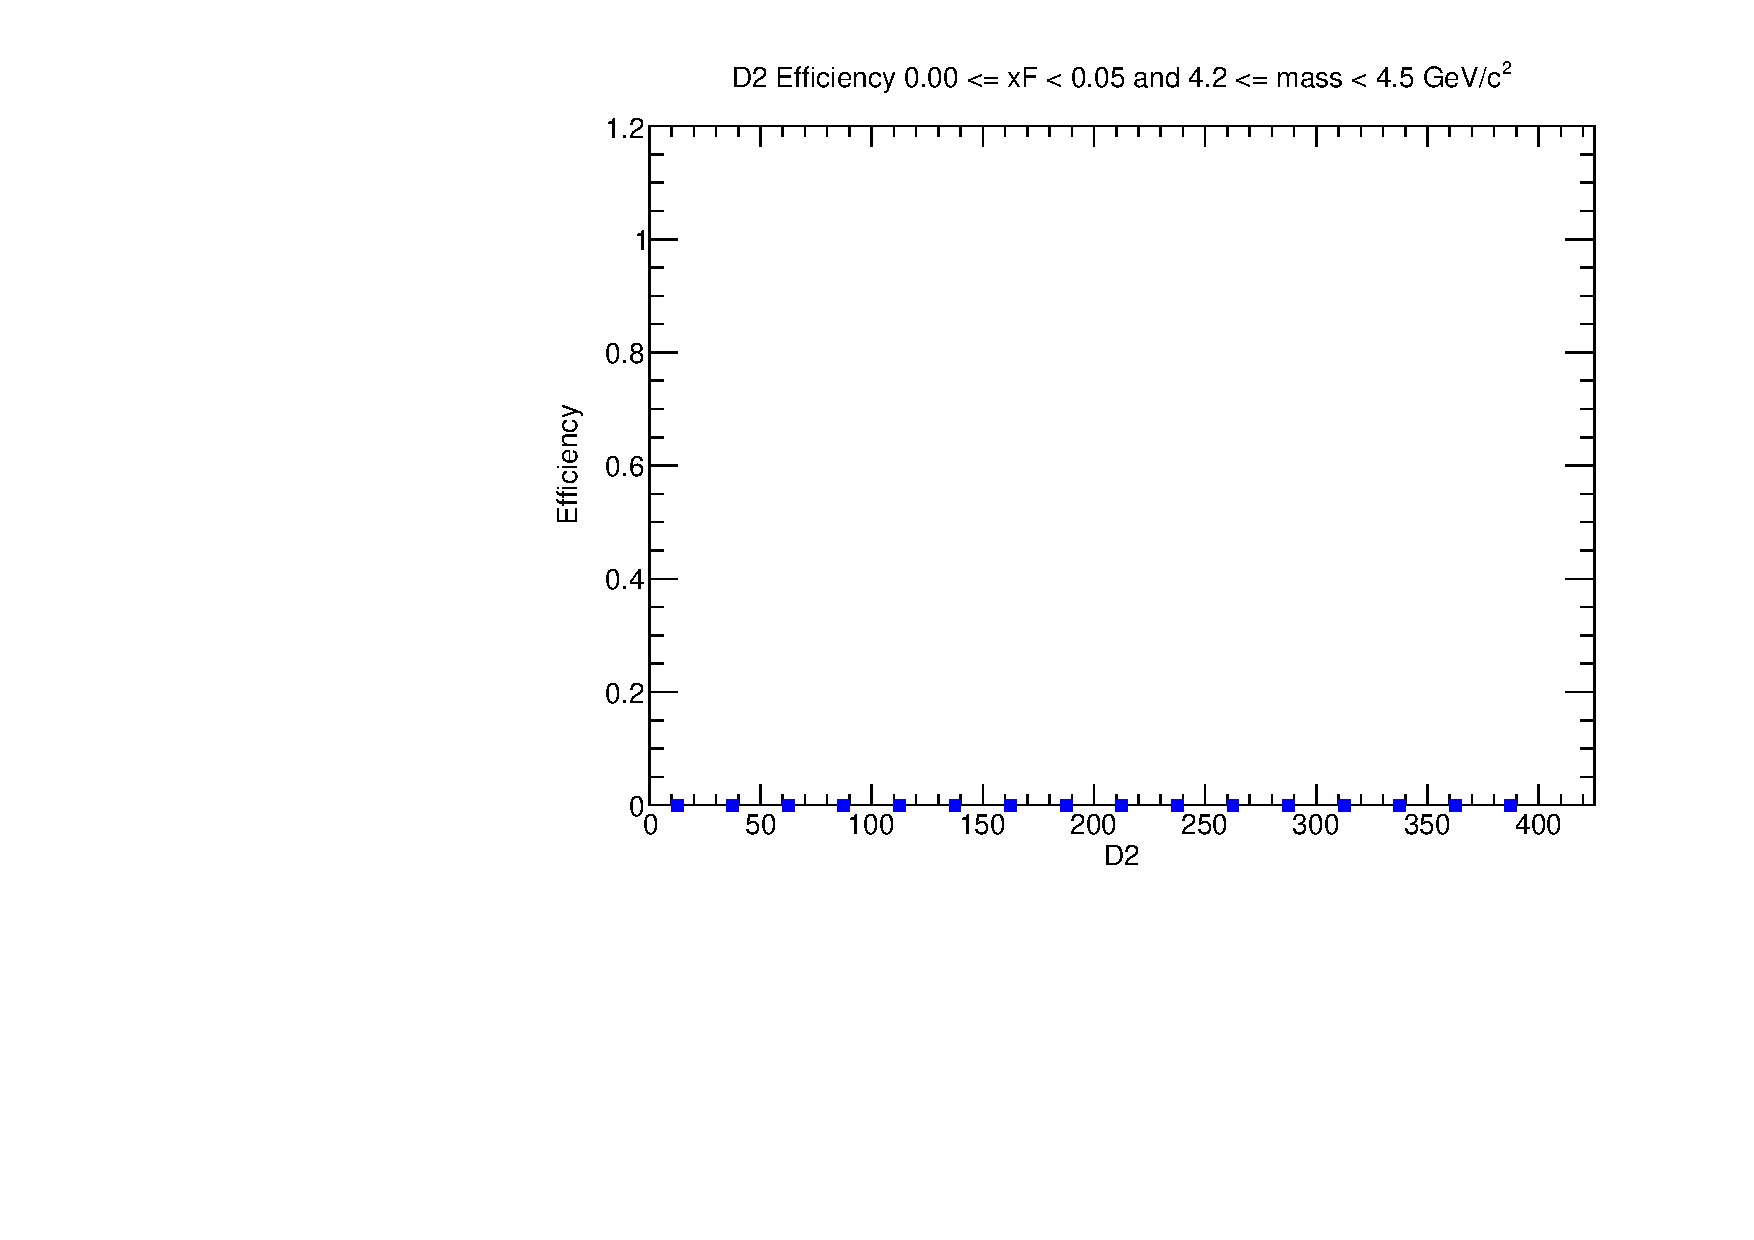
\includegraphics[width=\textwidth]{./kTrackerEfficiencyPlots/D2_Efficiency_xF0_mass0.pdf}
        \caption{$4.2 \leq m < 4.5$ GeV/$c^2$}
        \label{fig:xF0_mass0}
    \end{subfigure}
    \hfill
    \begin{subfigure}[b]{0.32\textwidth}
        \centering
        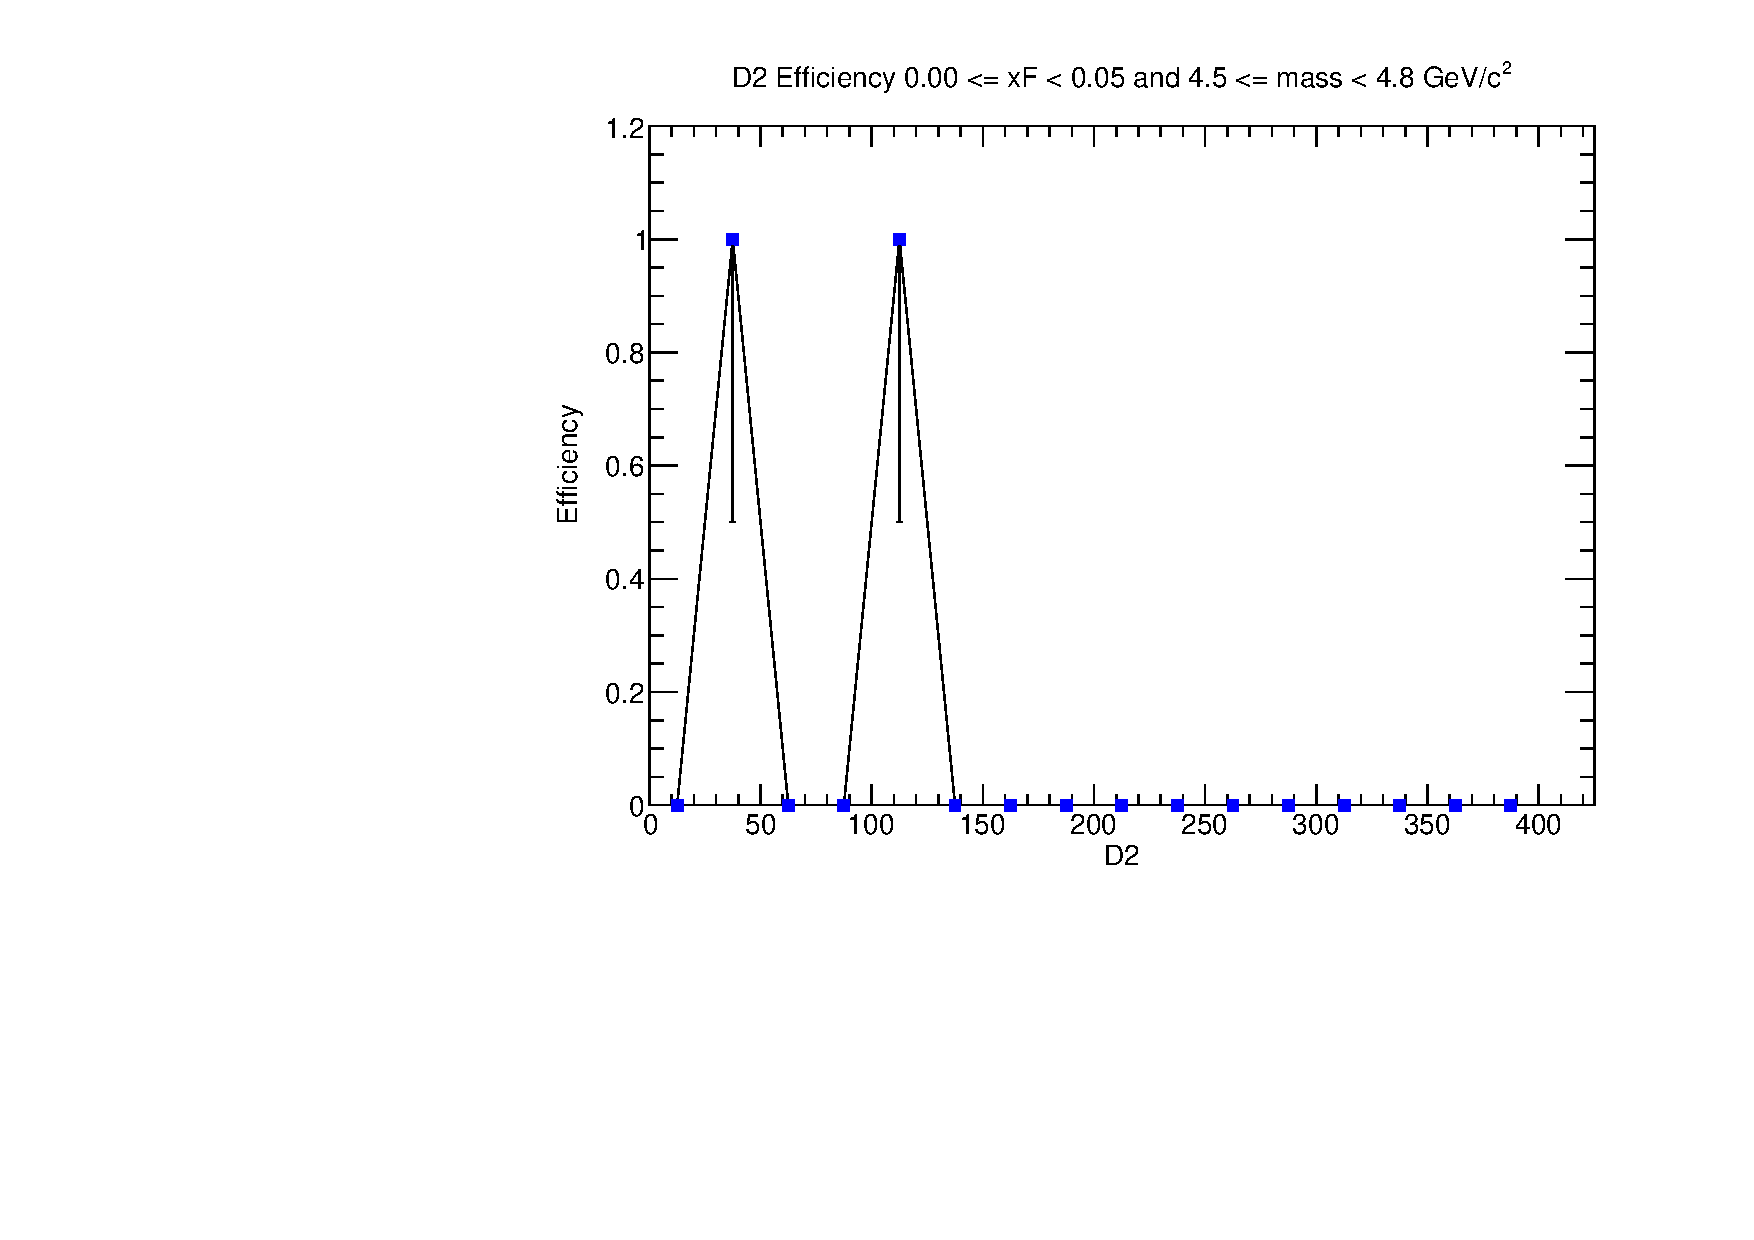
\includegraphics[width=\textwidth]{./kTrackerEfficiencyPlots/D2_Efficiency_xF0_mass1.pdf}
        \caption{$4.5 \leq m < 4.8$ GeV/$c^2$}
        \label{fig:xF0_mass1}
    \end{subfigure}
    \hfill
    \begin{subfigure}[b]{0.32\textwidth}
        \centering
        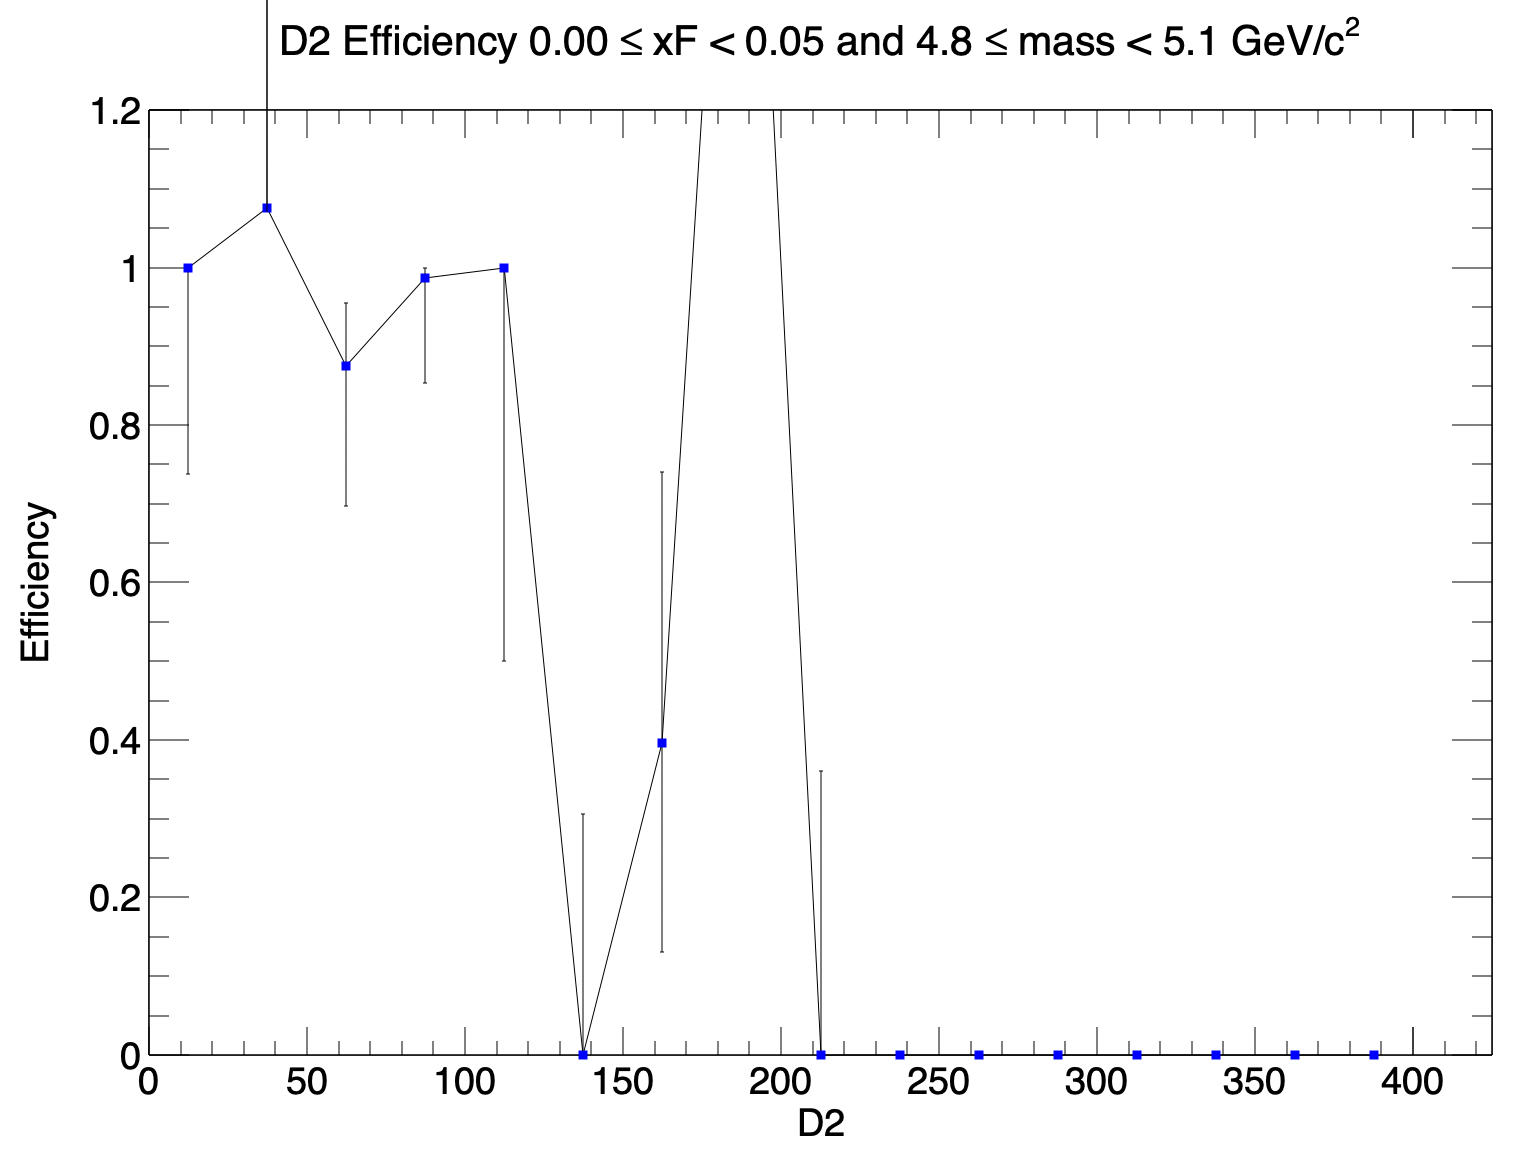
\includegraphics[width=\textwidth]{./kTrackerEfficiencyPlots/D2_Efficiency_xF0_mass2.png}
        \caption{$4.8 \leq m < 5.1$ GeV/$c^2$}
        \label{fig:xF0_mass2}
    \end{subfigure}
    \vspace{0.5cm}
    \begin{subfigure}[b]{0.32\textwidth}
        \centering
        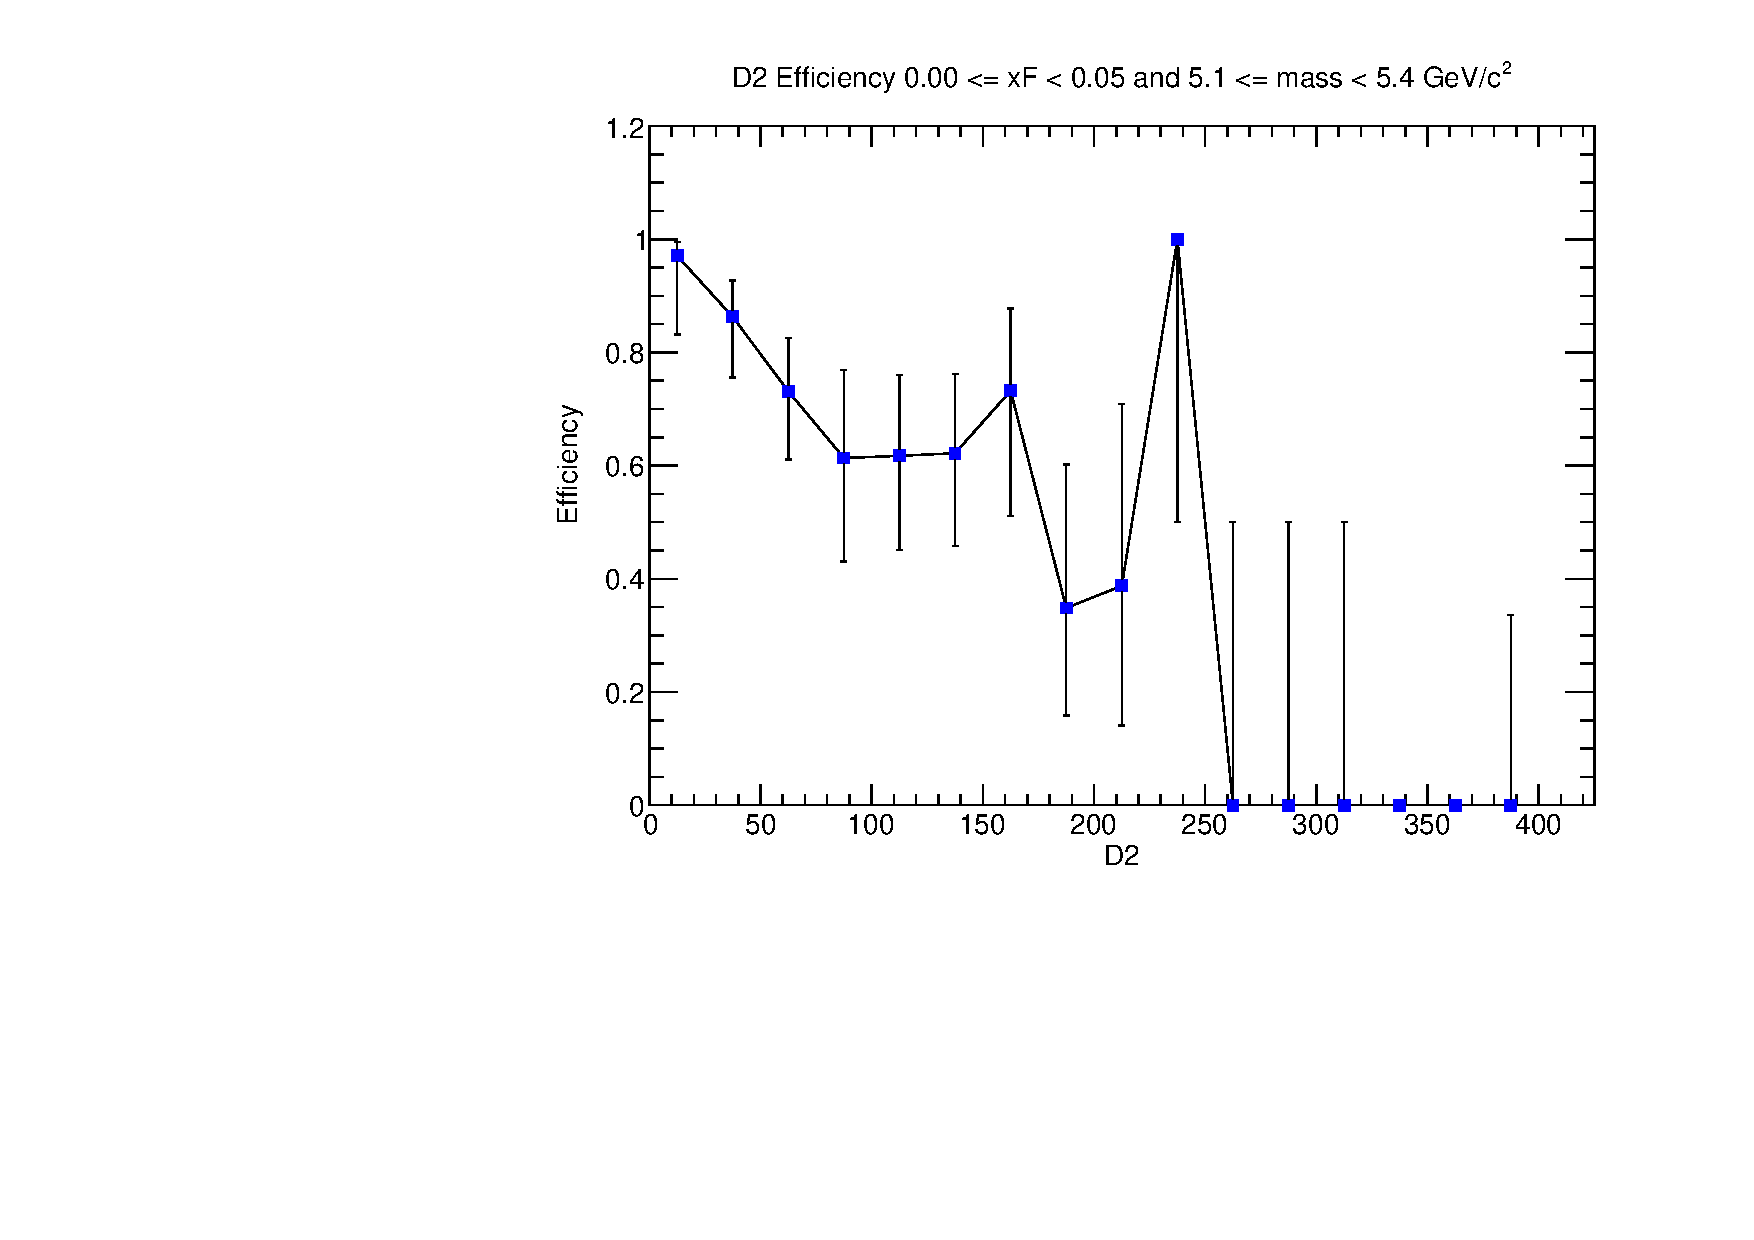
\includegraphics[width=\textwidth]{./kTrackerEfficiencyPlots/D2_Efficiency_xF0_mass3.pdf}
        \caption{$5.1 \leq m < 5.4$ GeV/$c^2$}
        \label{fig:xF0_mass3}
    \end{subfigure}
    \hfill
    \begin{subfigure}[b]{0.32\textwidth}
        \centering
        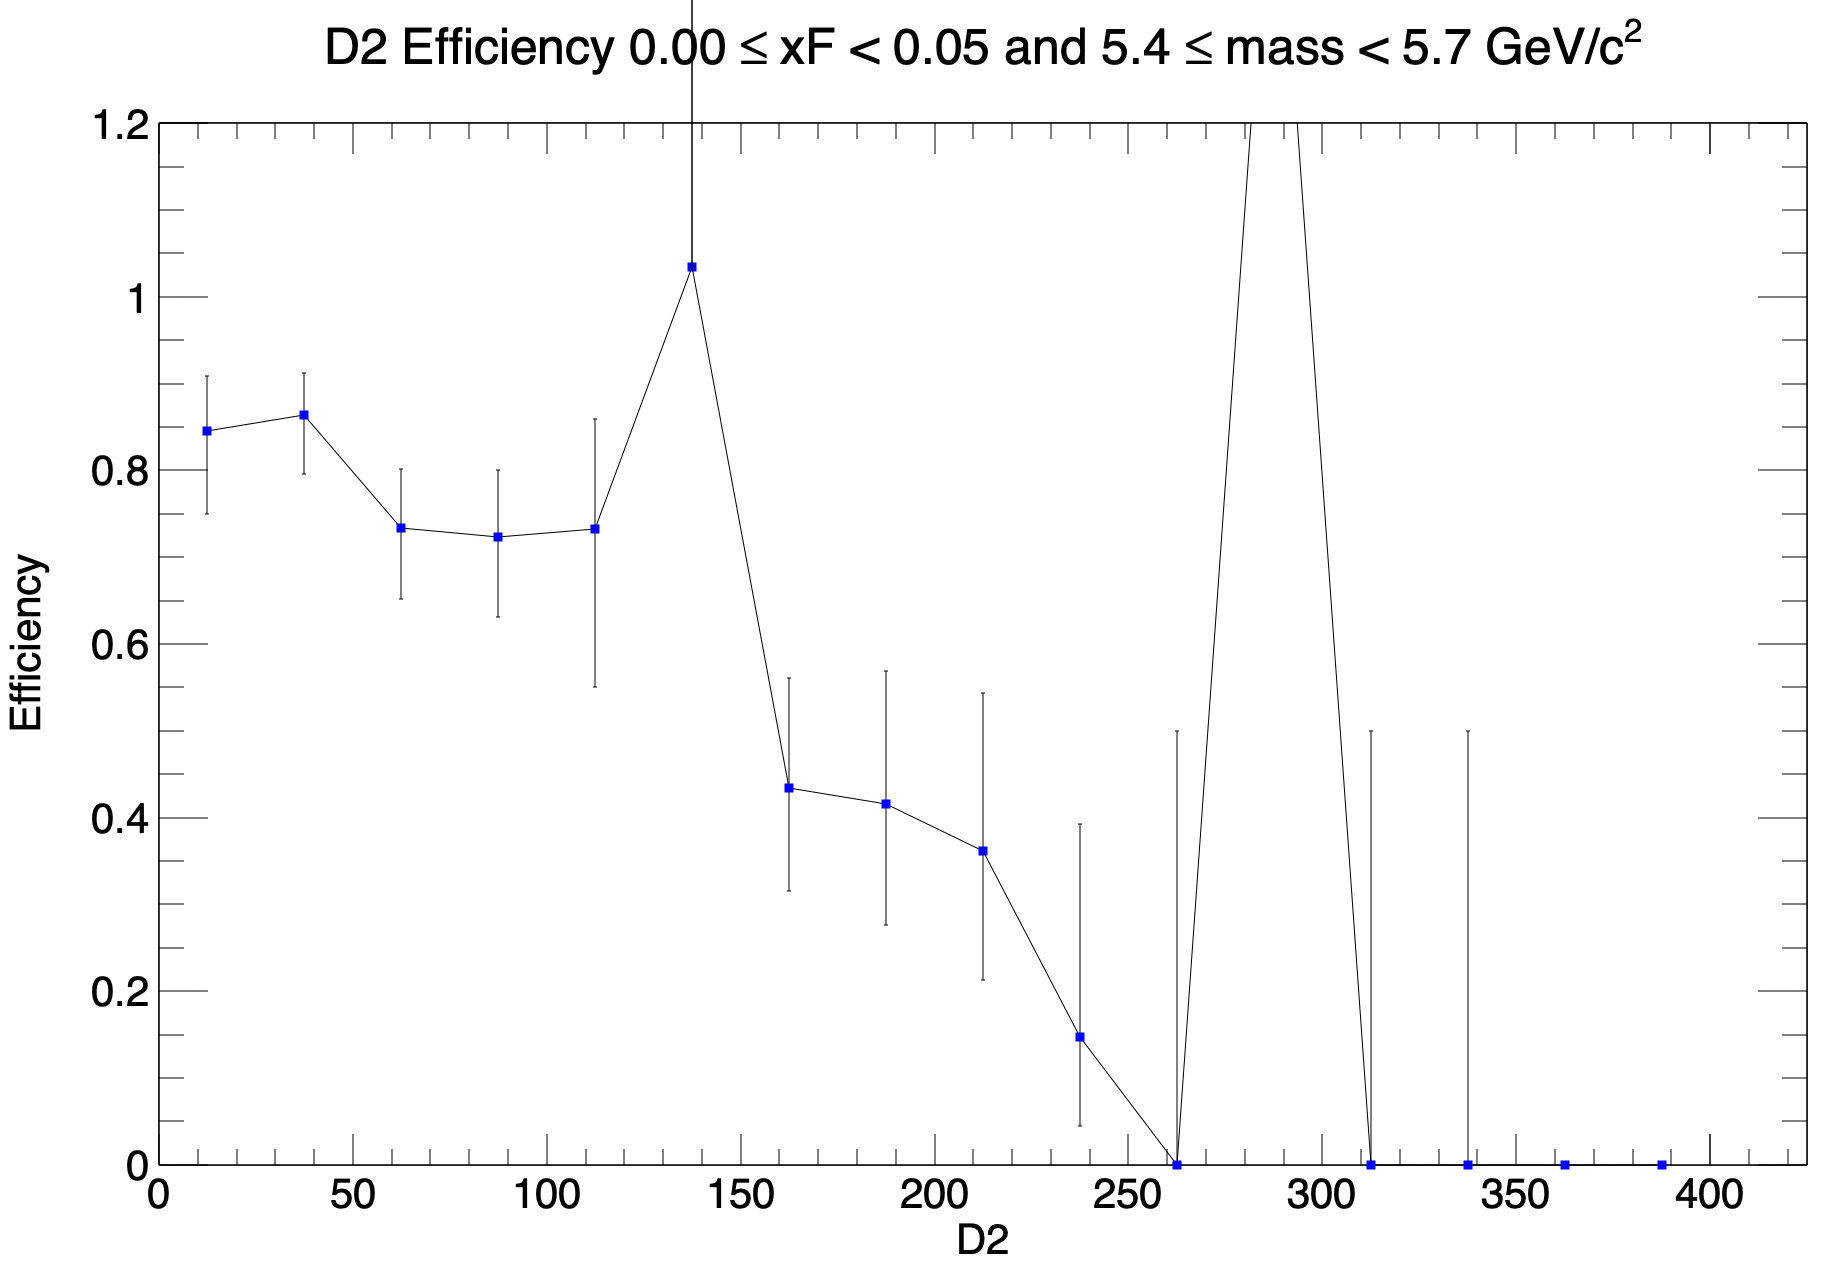
\includegraphics[width=\textwidth]{./kTrackerEfficiencyPlots/D2_Efficiency_xF0_mass4.png}
        \caption{$5.4 \leq m < 5.7$ GeV/$c^2$}
        \label{fig:xF0_mass4}
    \end{subfigure}
    \hfill
    \begin{subfigure}[b]{0.32\textwidth}
        \centering
        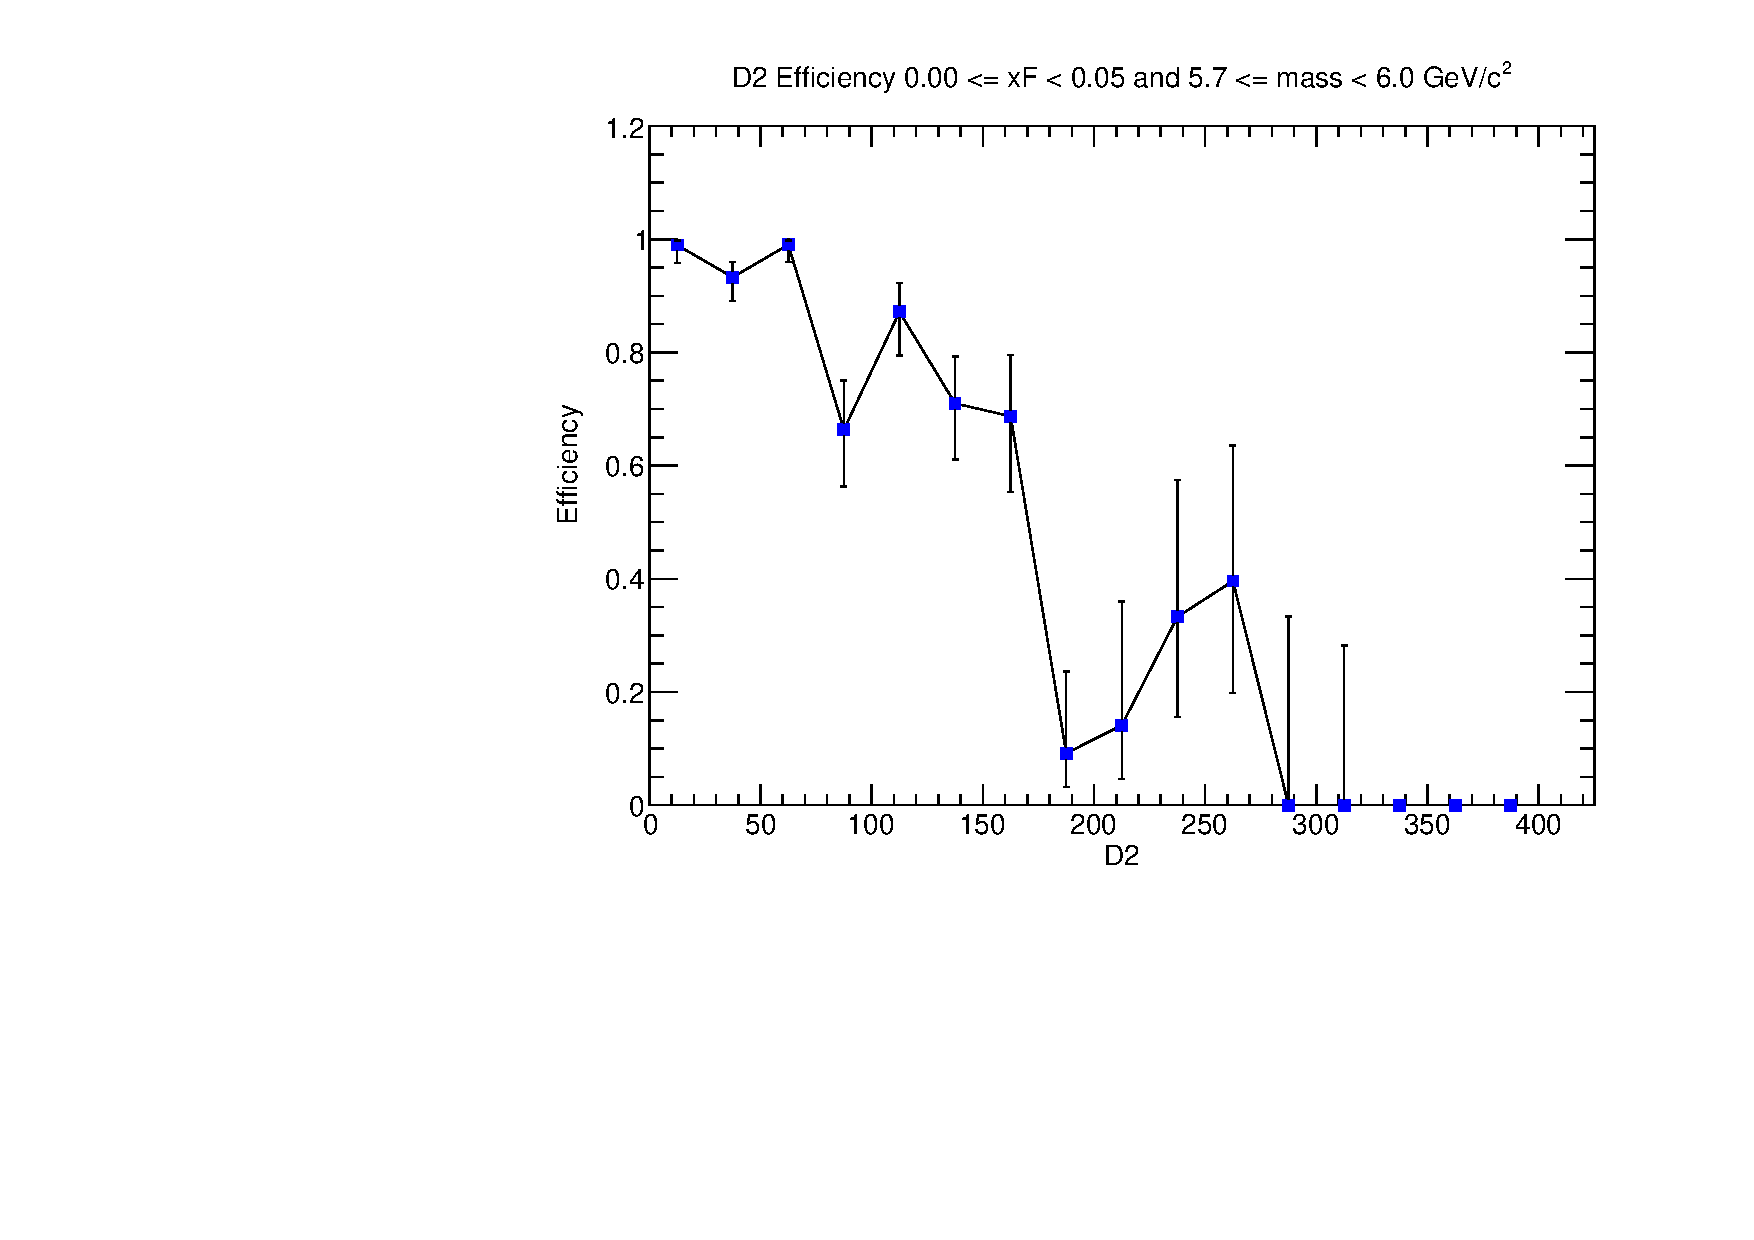
\includegraphics[width=\textwidth]{./kTrackerEfficiencyPlots/D2_Efficiency_xF0_mass5.pdf}
        \caption{$5.7 \leq m < 6.0$ GeV/$c^2$}
        \label{fig:xF0_mass5}
    \end{subfigure}
    \vspace{0.5cm}
    \begin{subfigure}[b]{0.32\textwidth}
        \centering
        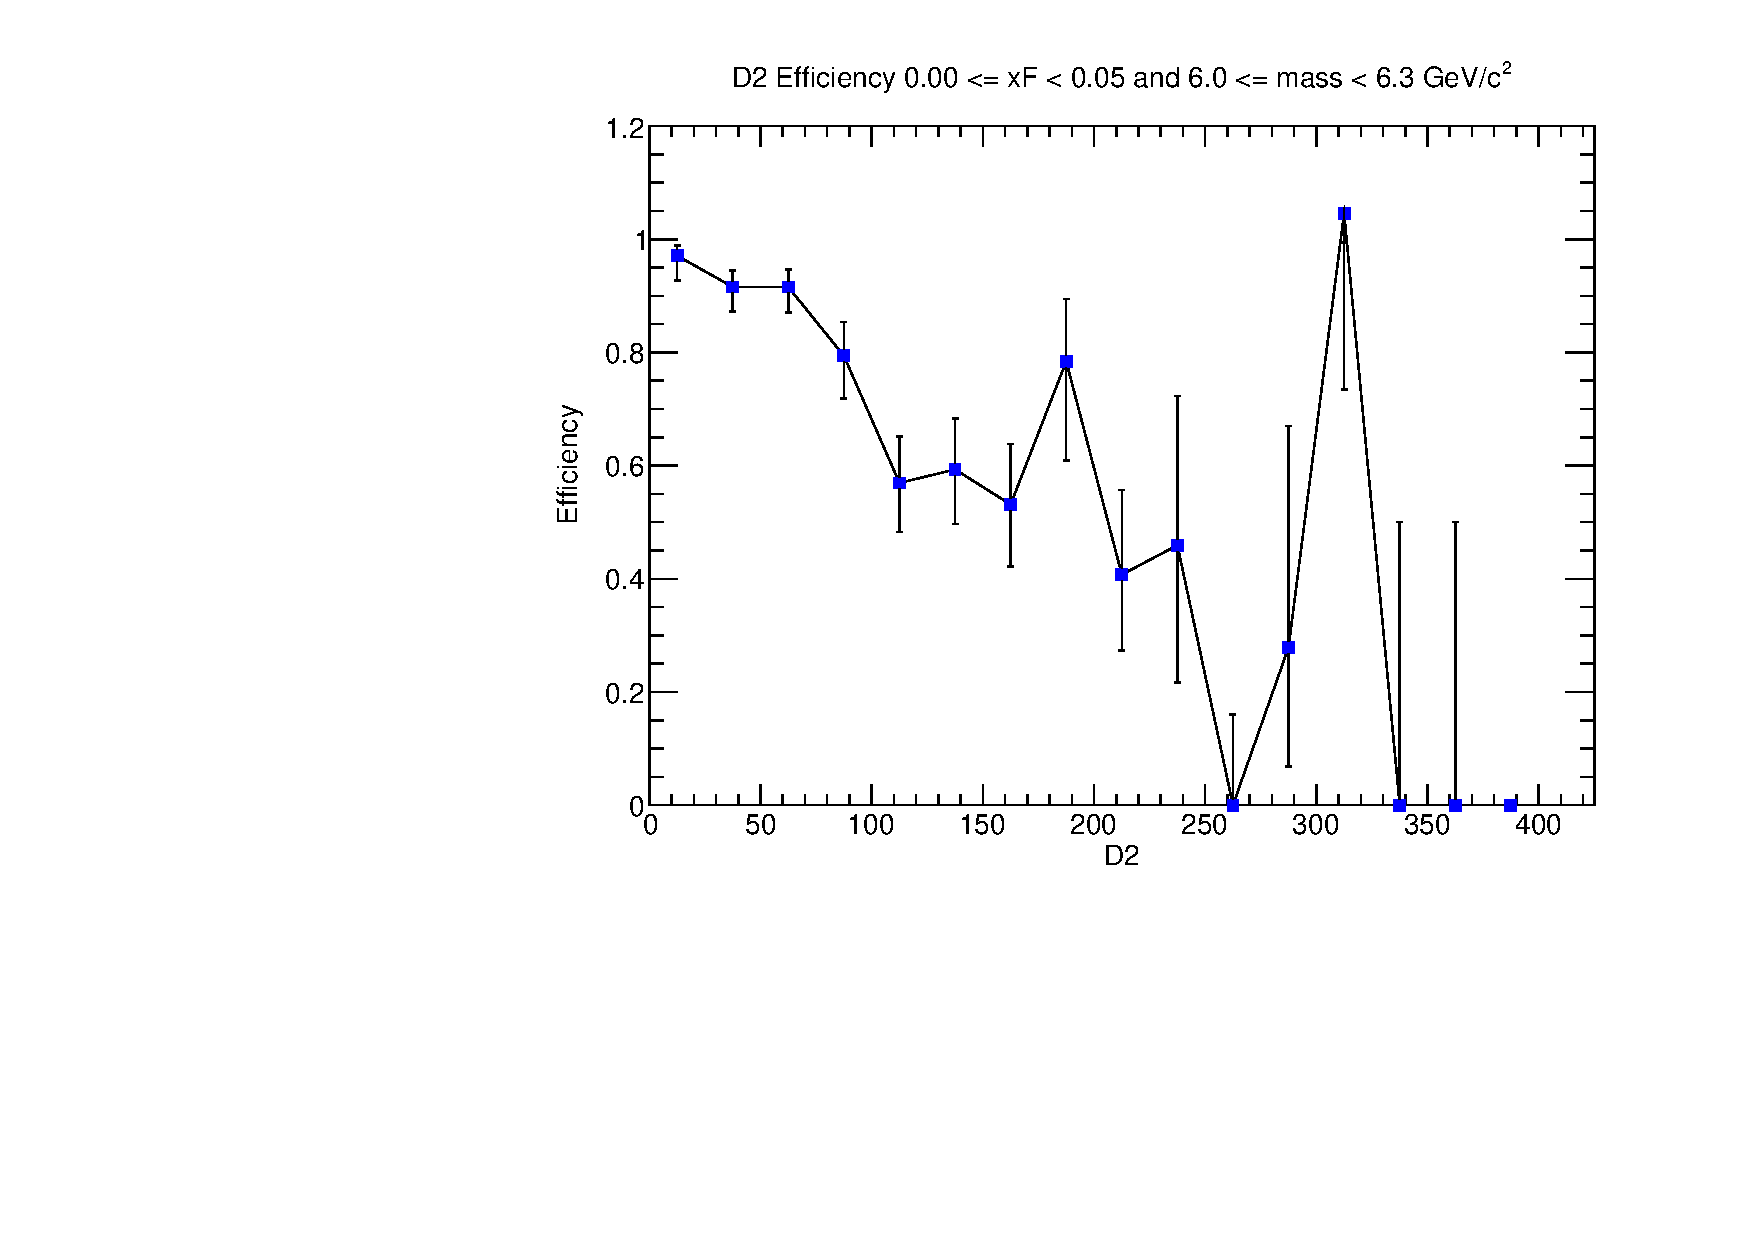
\includegraphics[width=\textwidth]{./kTrackerEfficiencyPlots/D2_Efficiency_xF0_mass6.pdf}
        \caption{$6.0 \leq m < 6.3$ GeV/$c^2$}
        \label{fig:xF0_mass6}
    \end{subfigure}
    \hfill
    \begin{subfigure}[b]{0.32\textwidth}
        \centering
        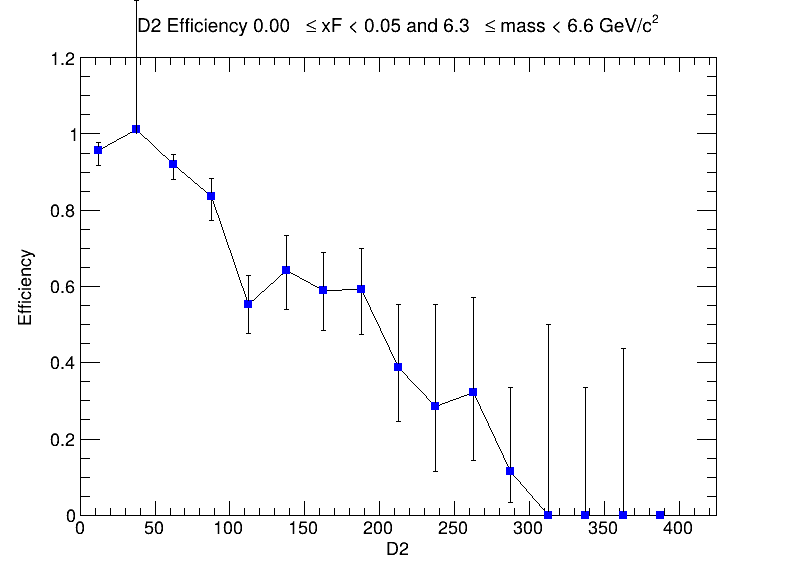
\includegraphics[width=\textwidth]{./kTrackerEfficiencyPlots/D2_Efficiency_xF0_mass7.png}
        \caption{$6.3 \leq m < 6.6$ GeV/$c^2$}
        \label{fig:xF0_mass7}
    \end{subfigure}
    \hfill
    \begin{subfigure}[b]{0.32\textwidth}
        \centering
        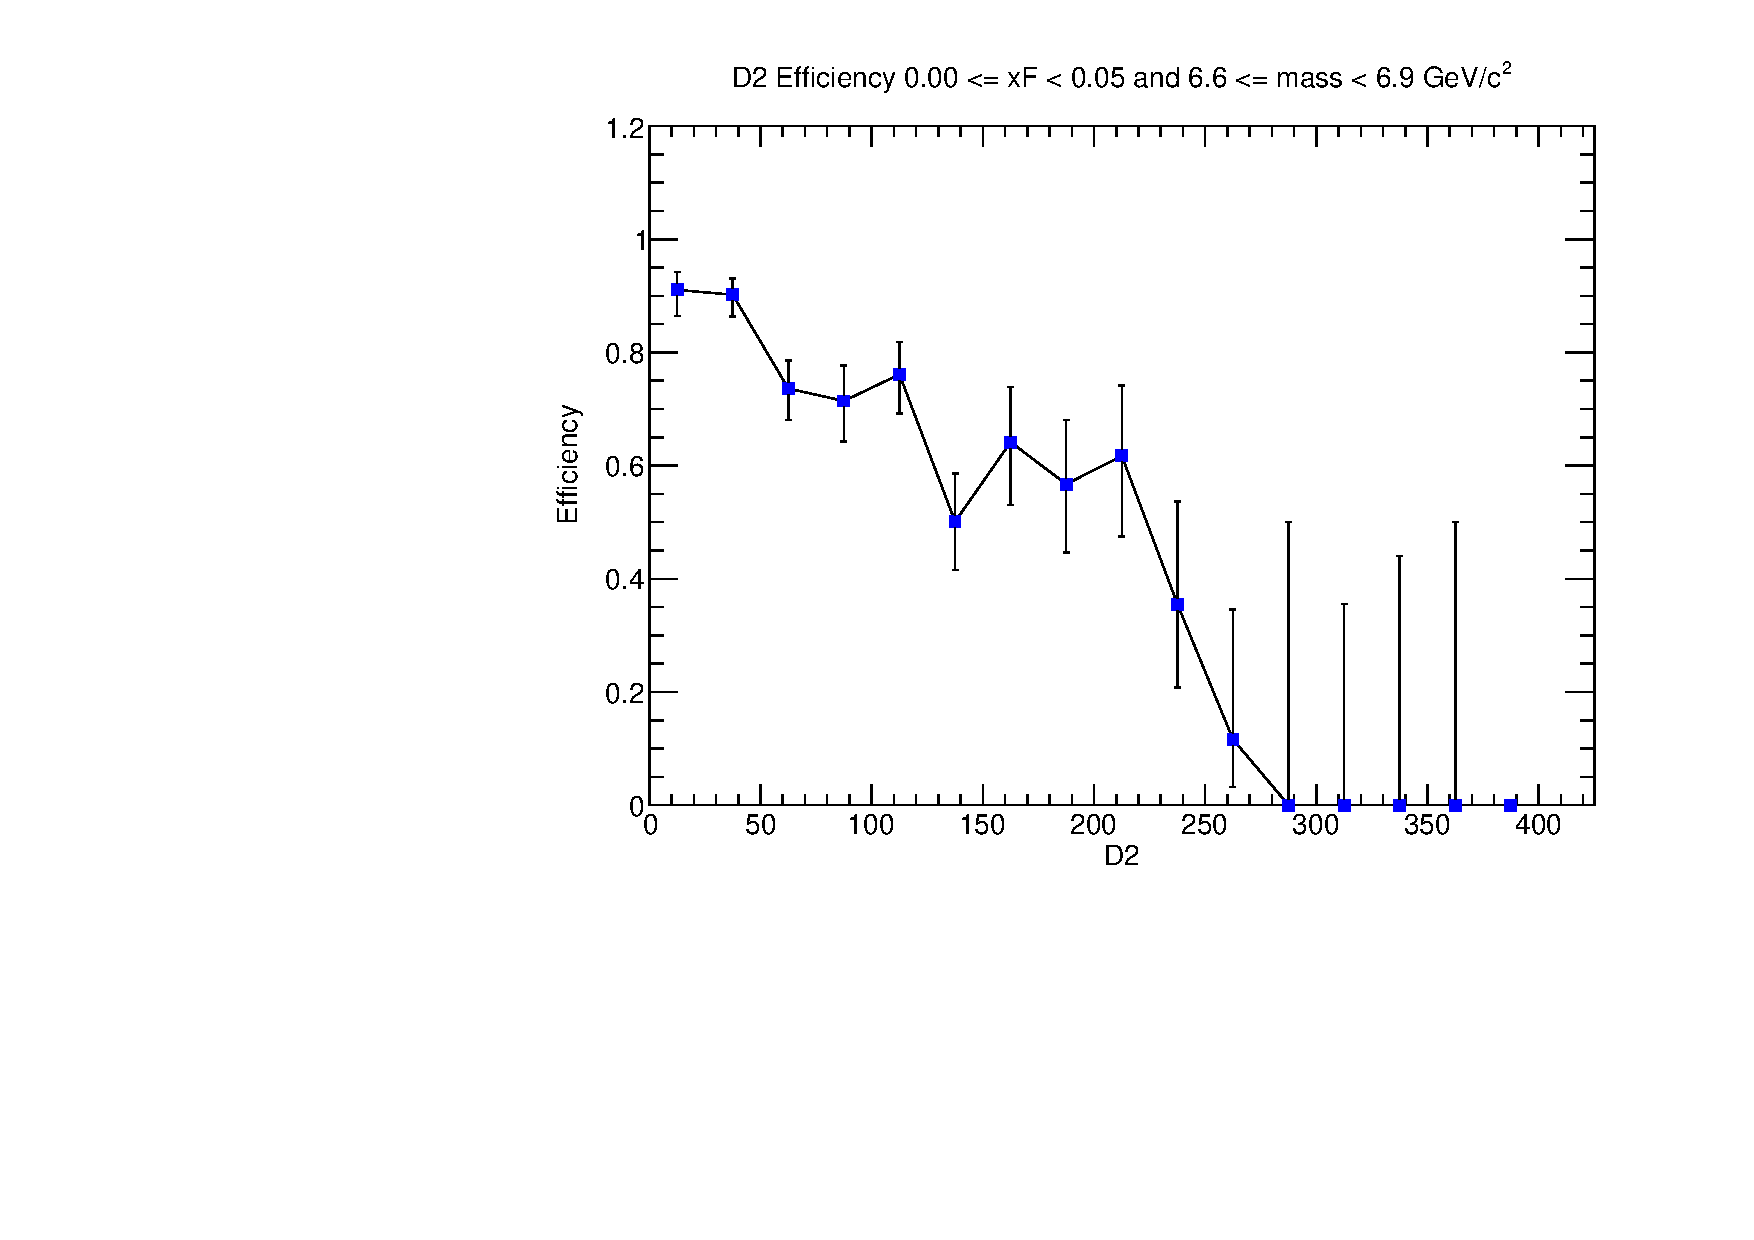
\includegraphics[width=\textwidth]{./kTrackerEfficiencyPlots/D2_Efficiency_xF0_mass8.pdf}
        \caption{$6.6 \leq m < 6.9$ GeV/$c^2$}
        \label{fig:xF0_mass8}
    \end{subfigure}
    \vspace{0.5cm}
    \begin{subfigure}[b]{0.32\textwidth}
        \centering
        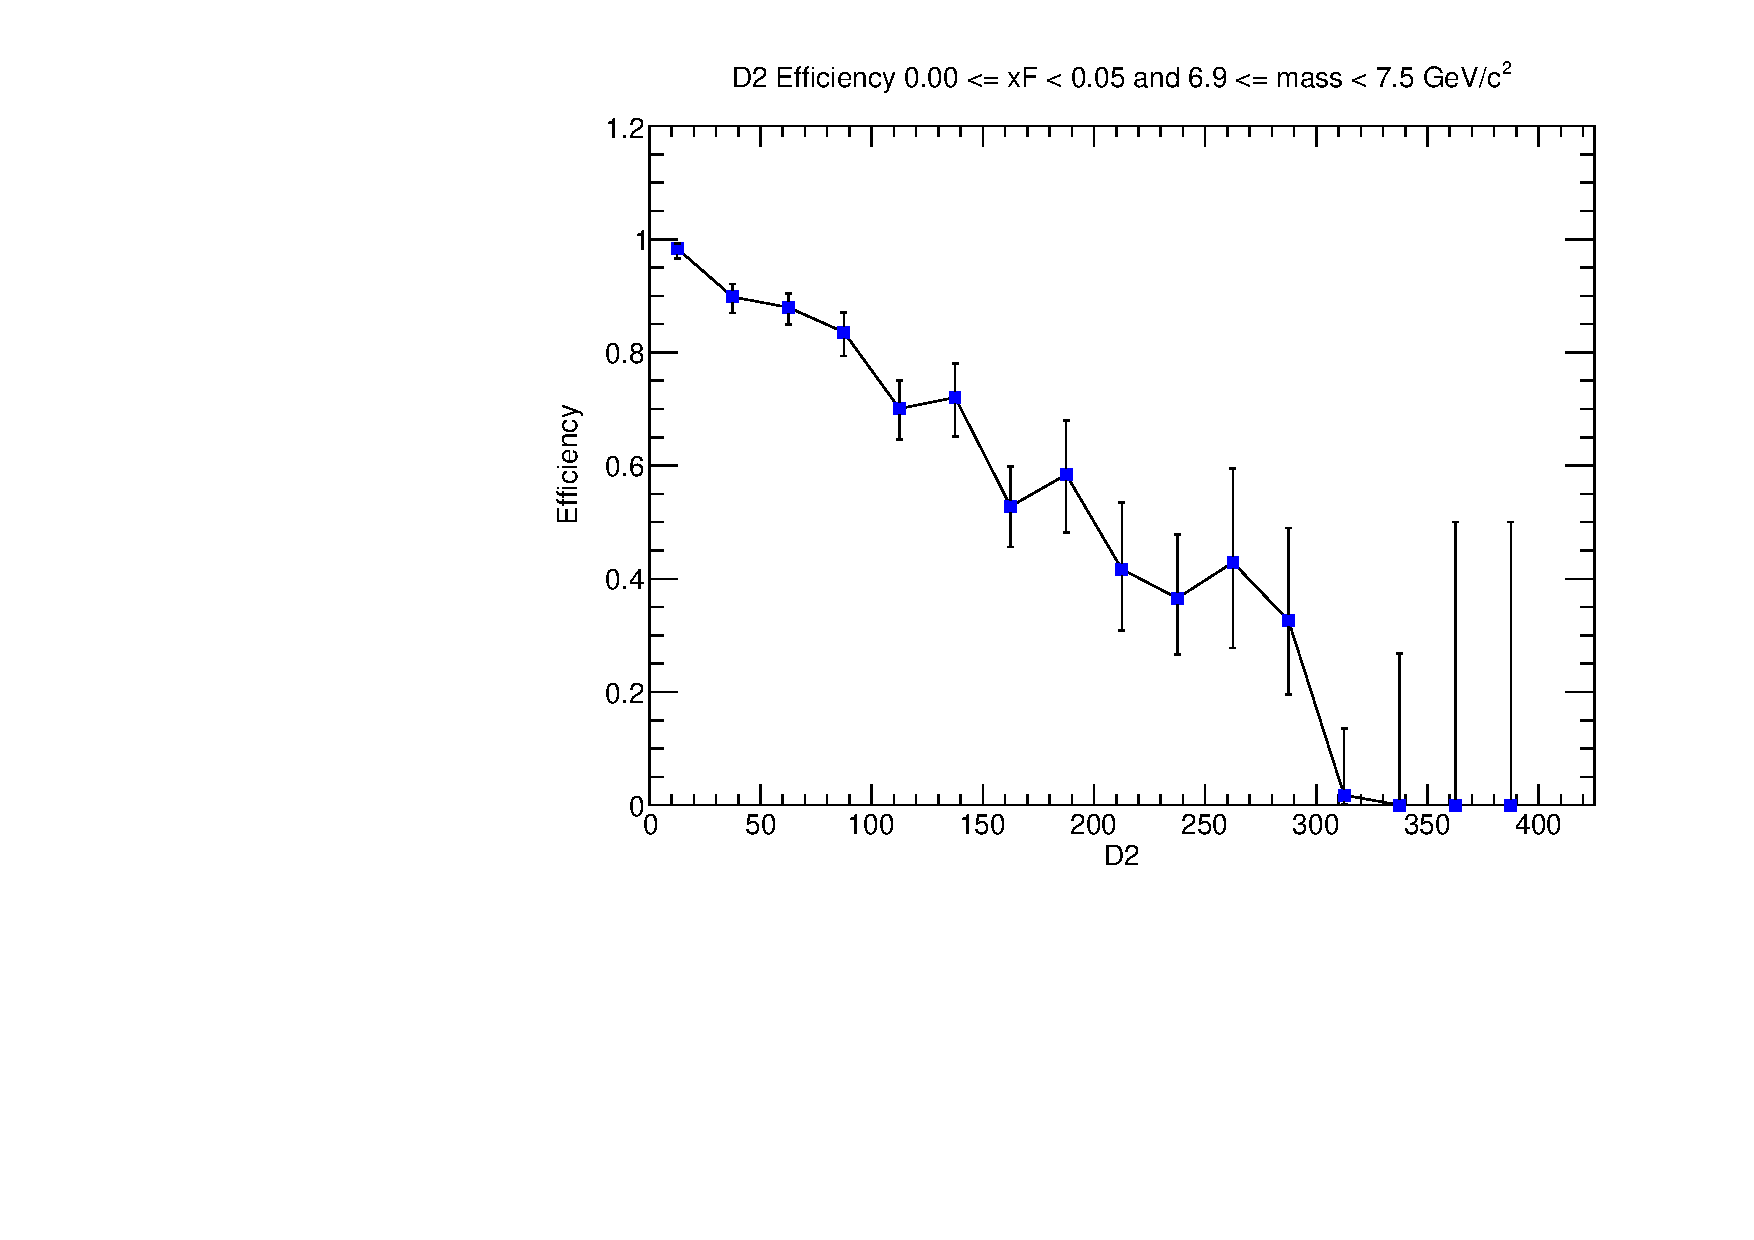
\includegraphics[width=\textwidth]{./kTrackerEfficiencyPlots/D2_Efficiency_xF0_mass9.pdf}
        \caption{$6.9 \leq m < 7.5$ GeV/$c^2$}
        \label{fig:xF0_mass9}
    \end{subfigure}
    \hfill
    \begin{subfigure}[b]{0.32\textwidth}
        \centering
        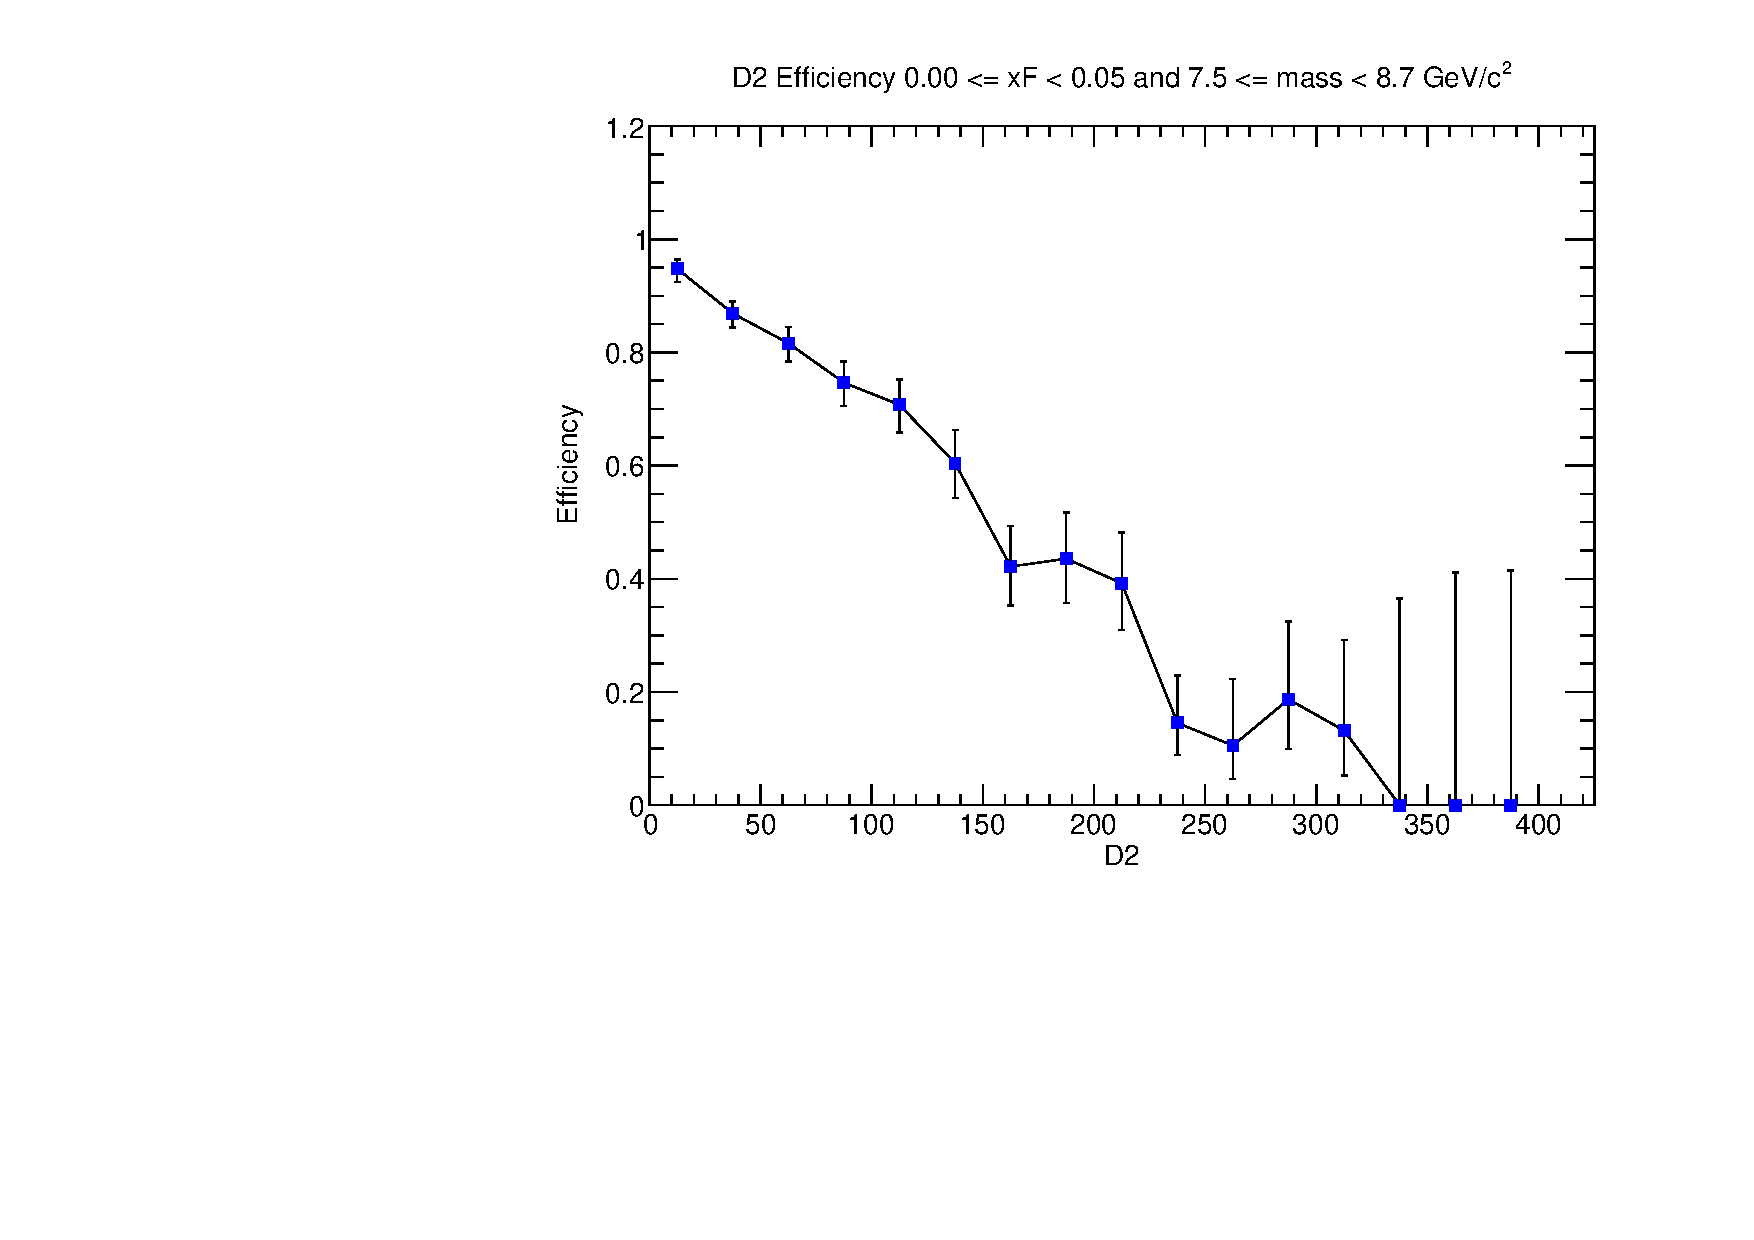
\includegraphics[width=\textwidth]{./kTrackerEfficiencyPlots/D2_Efficiency_xF0_mass10.pdf}
        \caption{$7.5 \leq m < 8.7$ GeV/$c^2$}
        \label{fig:xF0_mass10}
    \end{subfigure}
    \hfill
    \caption{Efficiency plots for the $x_F$ bin $0.00 \leq x_F < 0.05$.}
    \label{fig:xF0}
\end{figure}

\clearpage

\begin{figure}[p]
    \centering
    \begin{subfigure}[b]{0.32\textwidth}
        \centering
        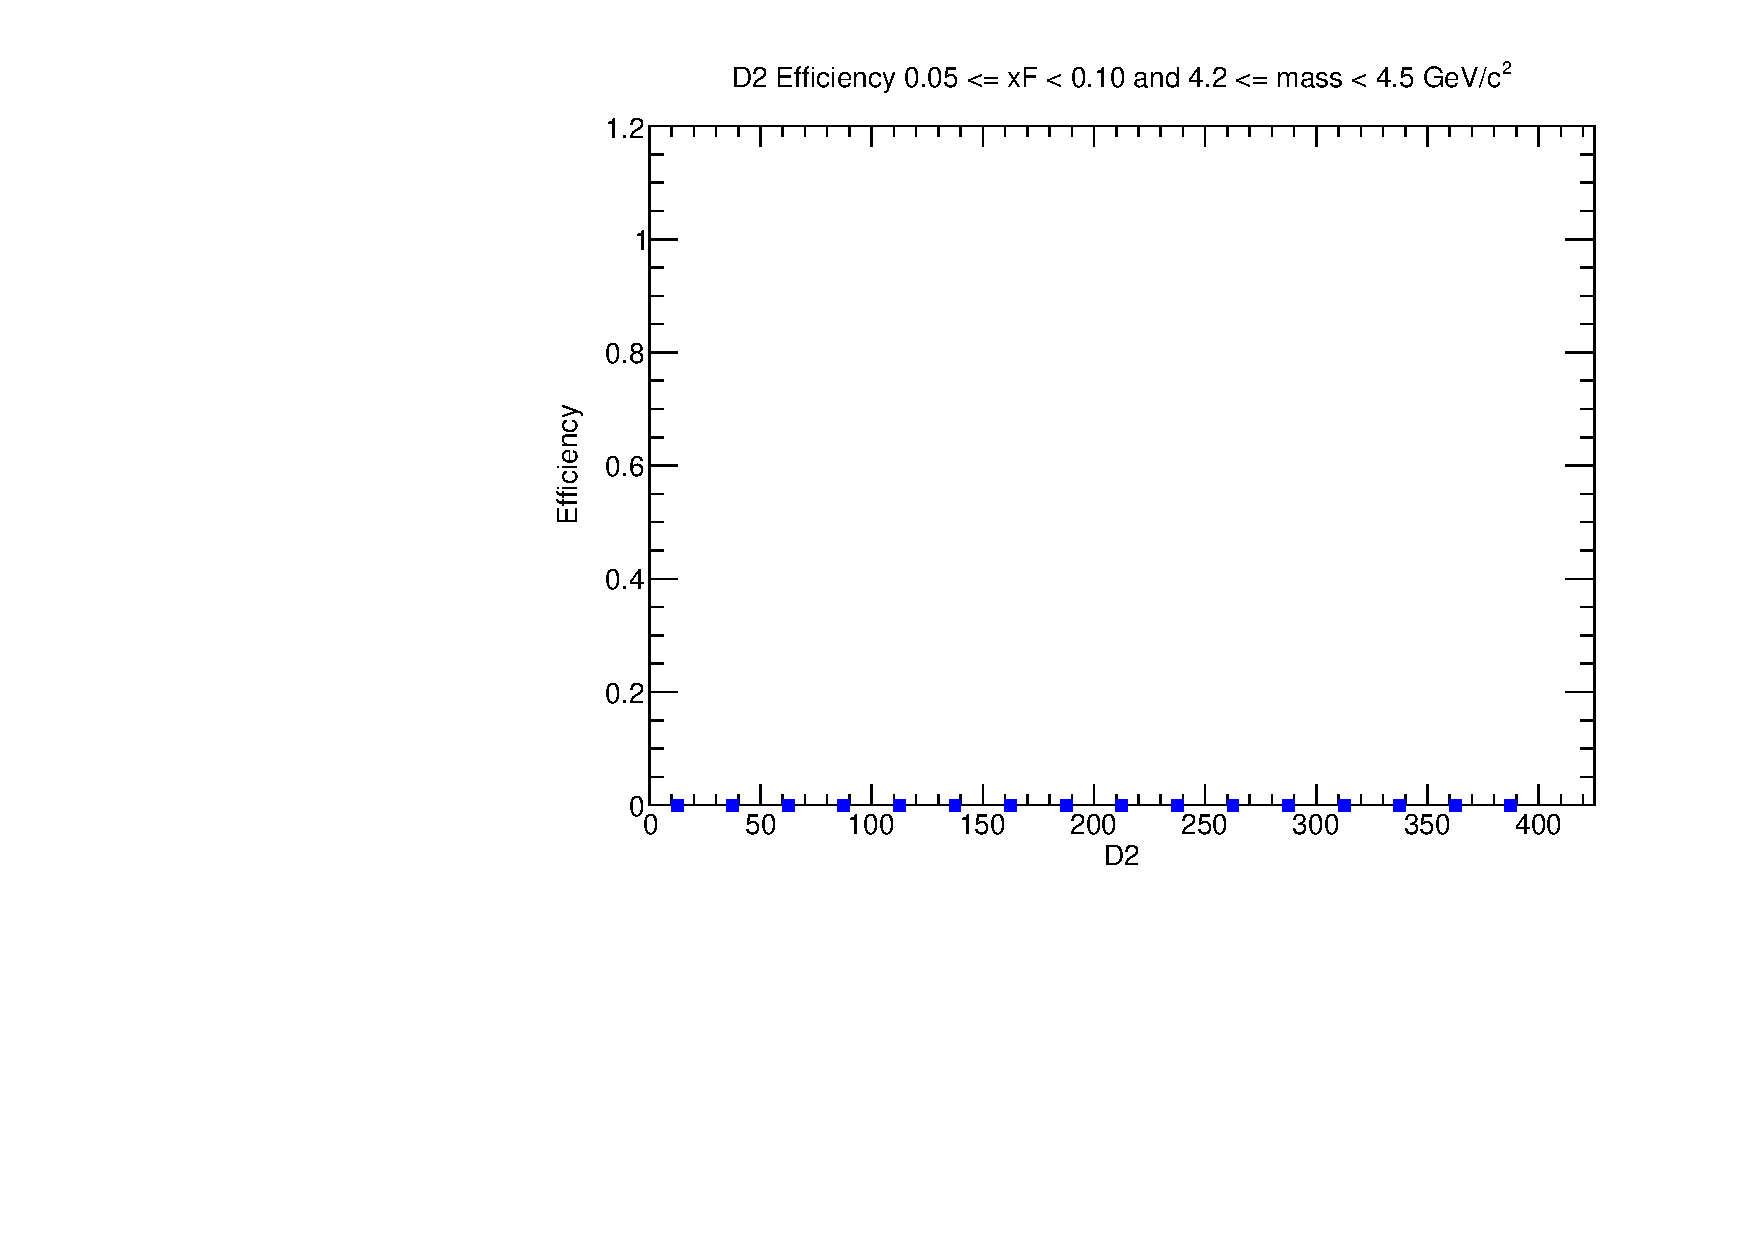
\includegraphics[width=\textwidth]{./kTrackerEfficiencyPlots/D2_Efficiency_xF1_mass0.pdf}
        \caption{$4.2 \leq m < 4.5$ GeV/$c^2$}
        \label{fig:xF1_mass0}
    \end{subfigure}
    \hfill
    \begin{subfigure}[b]{0.32\textwidth}
        \centering
        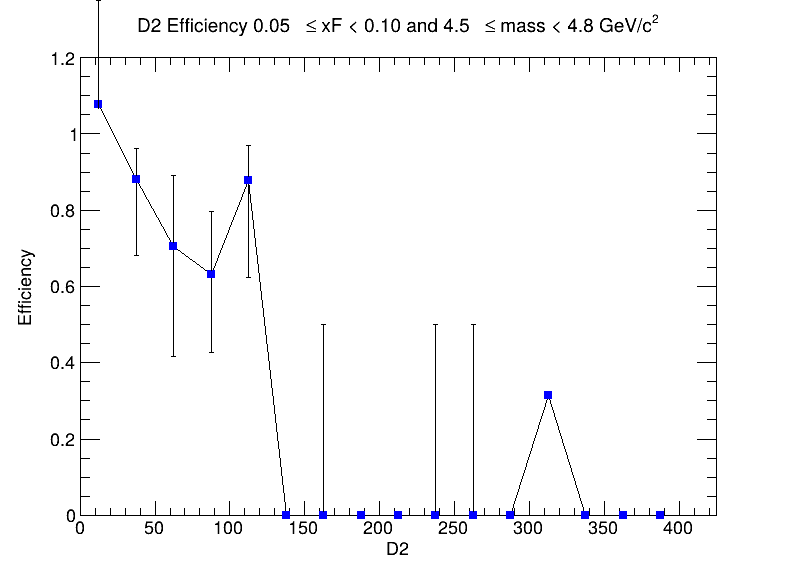
\includegraphics[width=\textwidth]{./kTrackerEfficiencyPlots/D2_Efficiency_xF1_mass1.png}
        \caption{$4.5 \leq m < 4.8$ GeV/$c^2$}
        \label{fig:xF1_mass1}
    \end{subfigure}
    \hfill
    \begin{subfigure}[b]{0.32\textwidth}
        \centering
        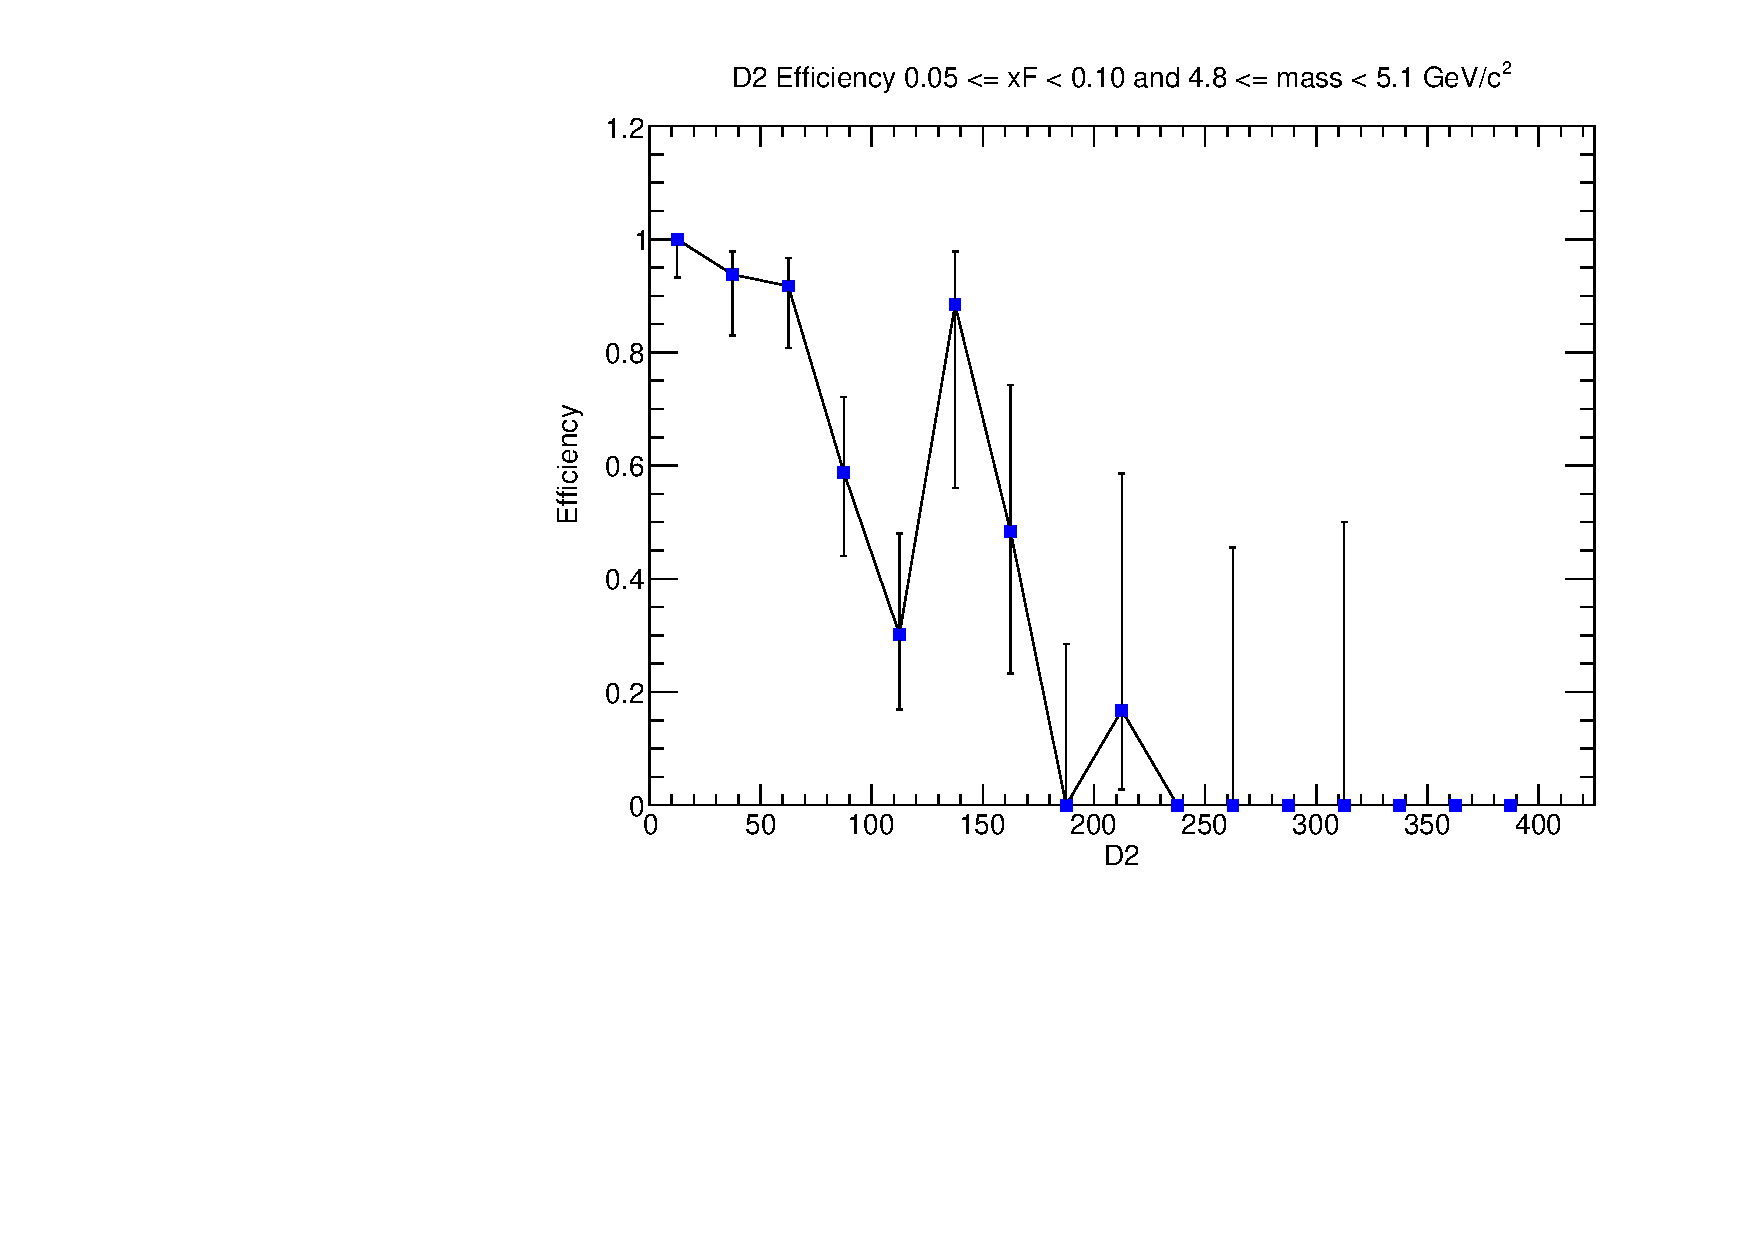
\includegraphics[width=\textwidth]{./kTrackerEfficiencyPlots/D2_Efficiency_xF1_mass2.pdf}
        \caption{$4.8 \leq m < 5.1$ GeV/$c^2$}
        \label{fig:xF1_mass2}
    \end{subfigure}
    \vspace{0.5cm}
    \begin{subfigure}[b]{0.32\textwidth}
        \centering
        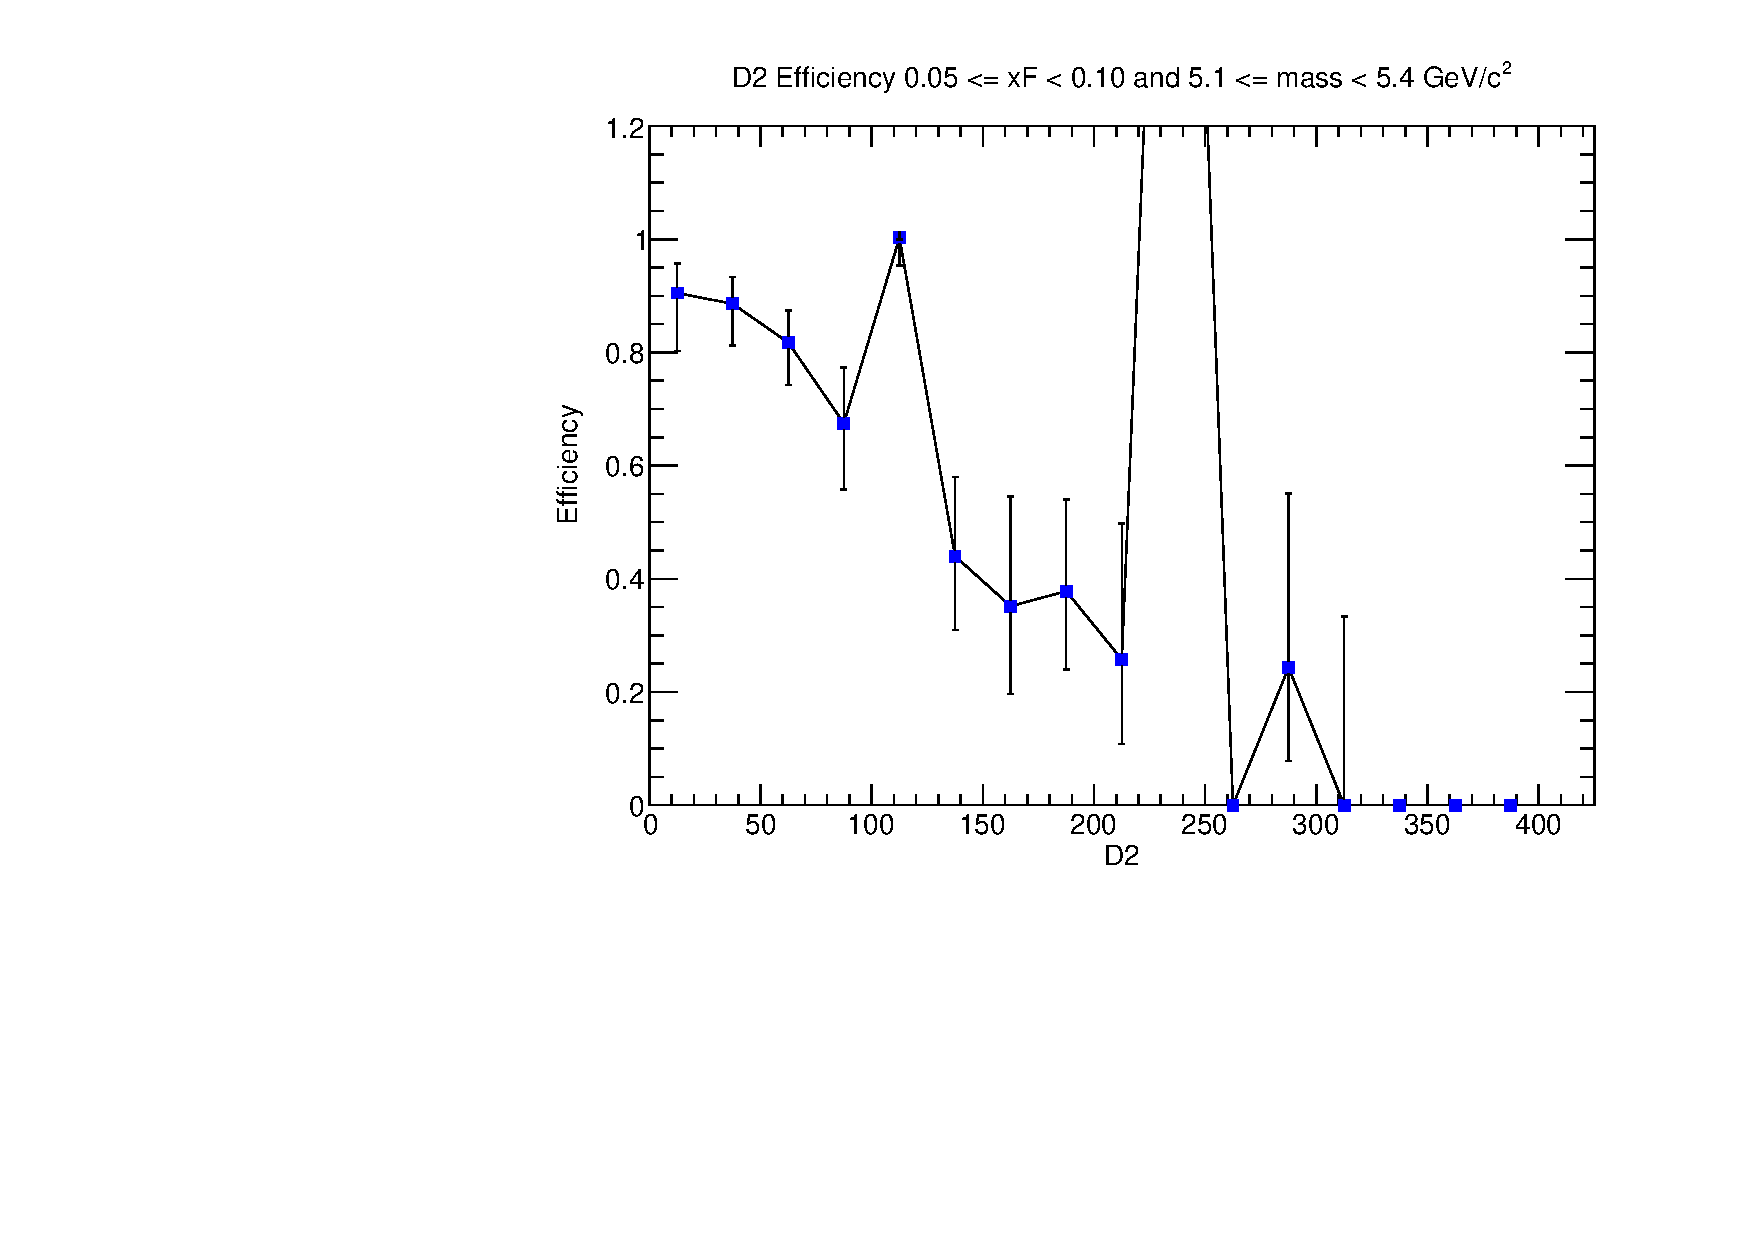
\includegraphics[width=\textwidth]{./kTrackerEfficiencyPlots/D2_Efficiency_xF1_mass3.pdf}
        \caption{$5.1 \leq m < 5.4$ GeV/$c^2$}
        \label{fig:xF1_mass3}
    \end{subfigure}
    \hfill
    \begin{subfigure}[b]{0.32\textwidth}
        \centering
        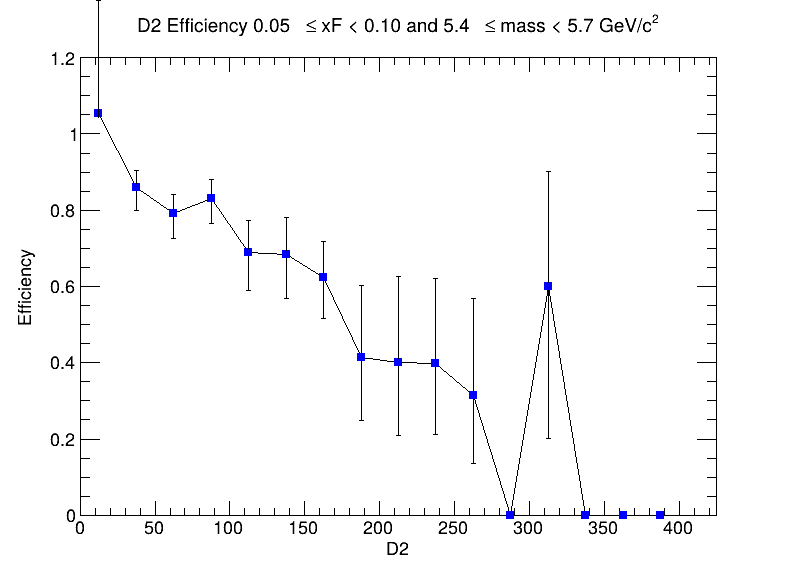
\includegraphics[width=\textwidth]{./kTrackerEfficiencyPlots/D2_Efficiency_xF1_mass4.png}
        \caption{$5.4 \leq m < 5.7$ GeV/$c^2$}
        \label{fig:xF1_mass4}
    \end{subfigure}
    \hfill
    \begin{subfigure}[b]{0.32\textwidth}
        \centering
        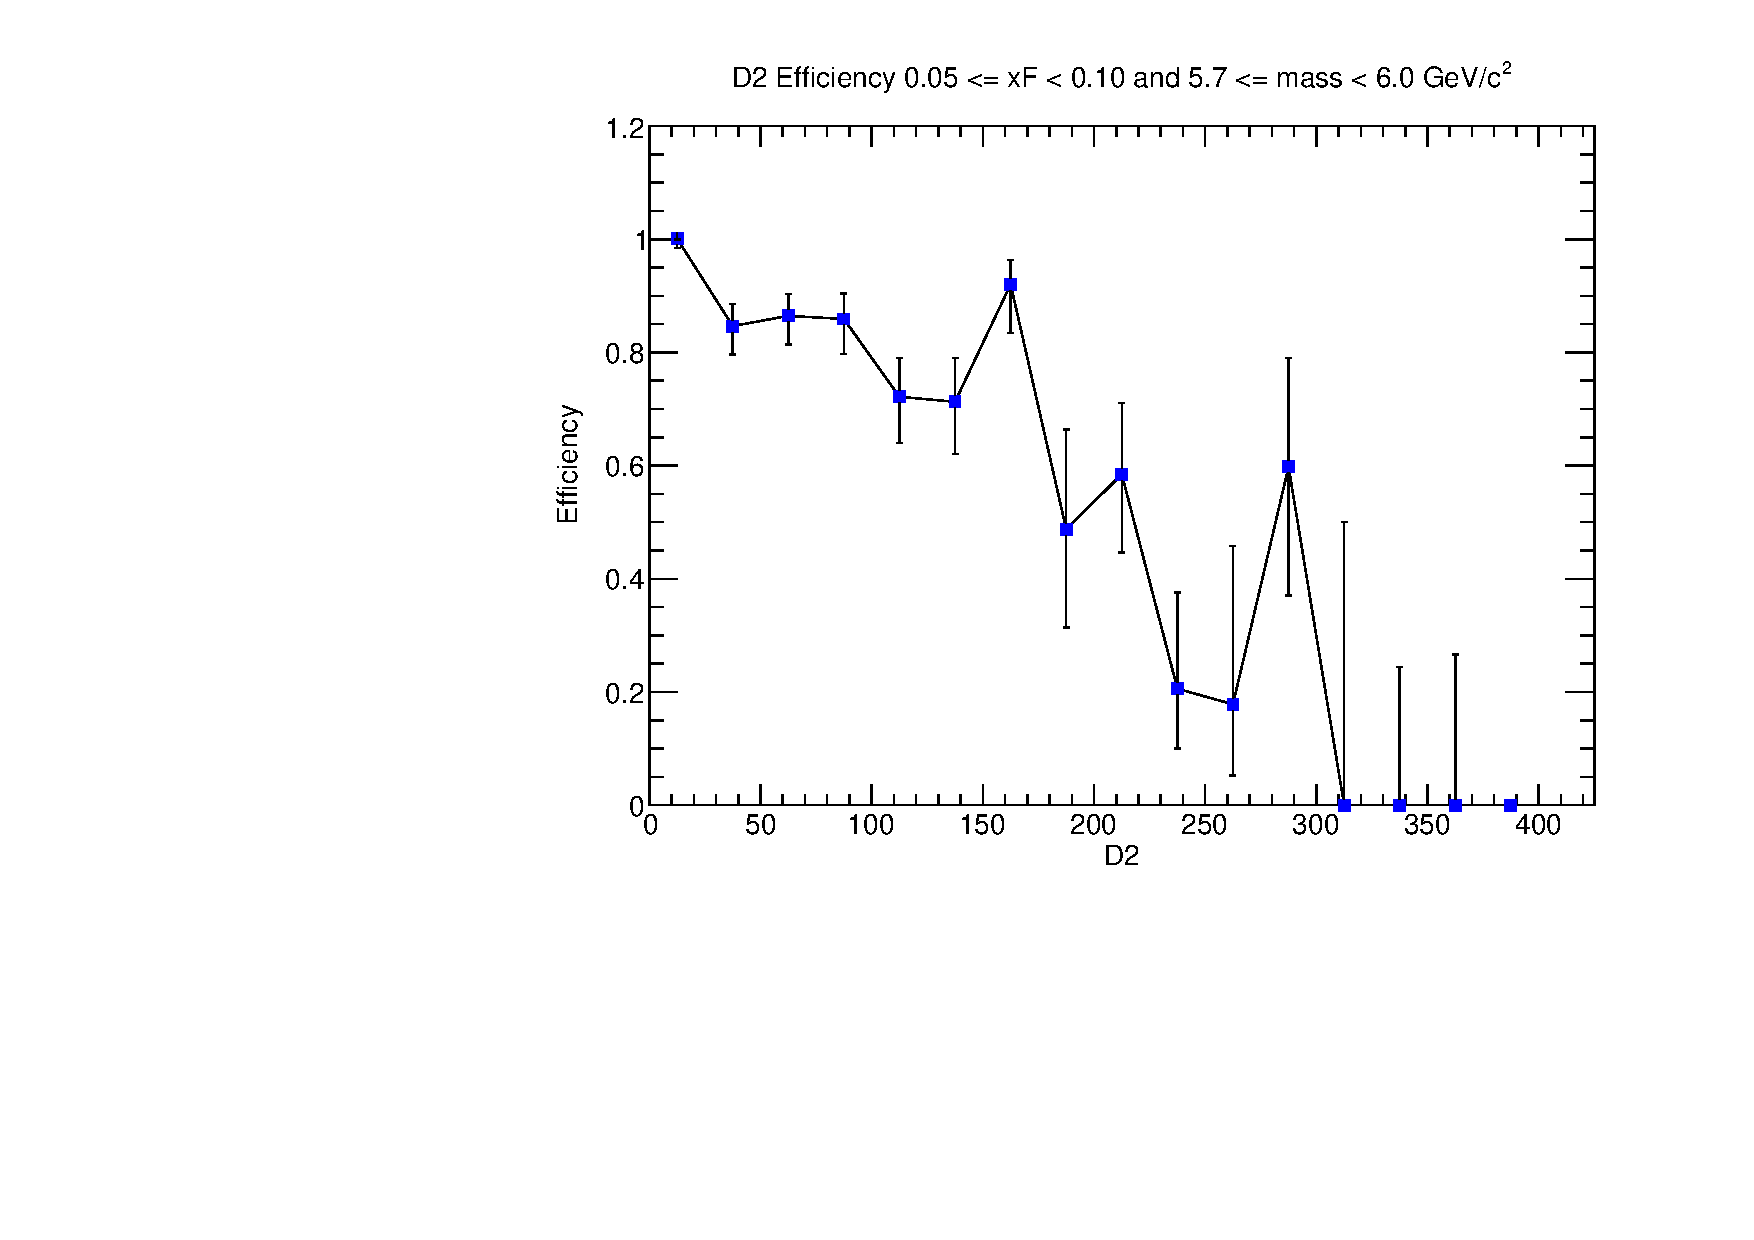
\includegraphics[width=\textwidth]{./kTrackerEfficiencyPlots/D2_Efficiency_xF1_mass5.pdf}
        \caption{$5.7 \leq m < 6.0$ GeV/$c^2$}
        \label{fig:xF1_mass5}
    \end{subfigure}
    \vspace{0.5cm}
    \begin{subfigure}[b]{0.32\textwidth}
        \centering
        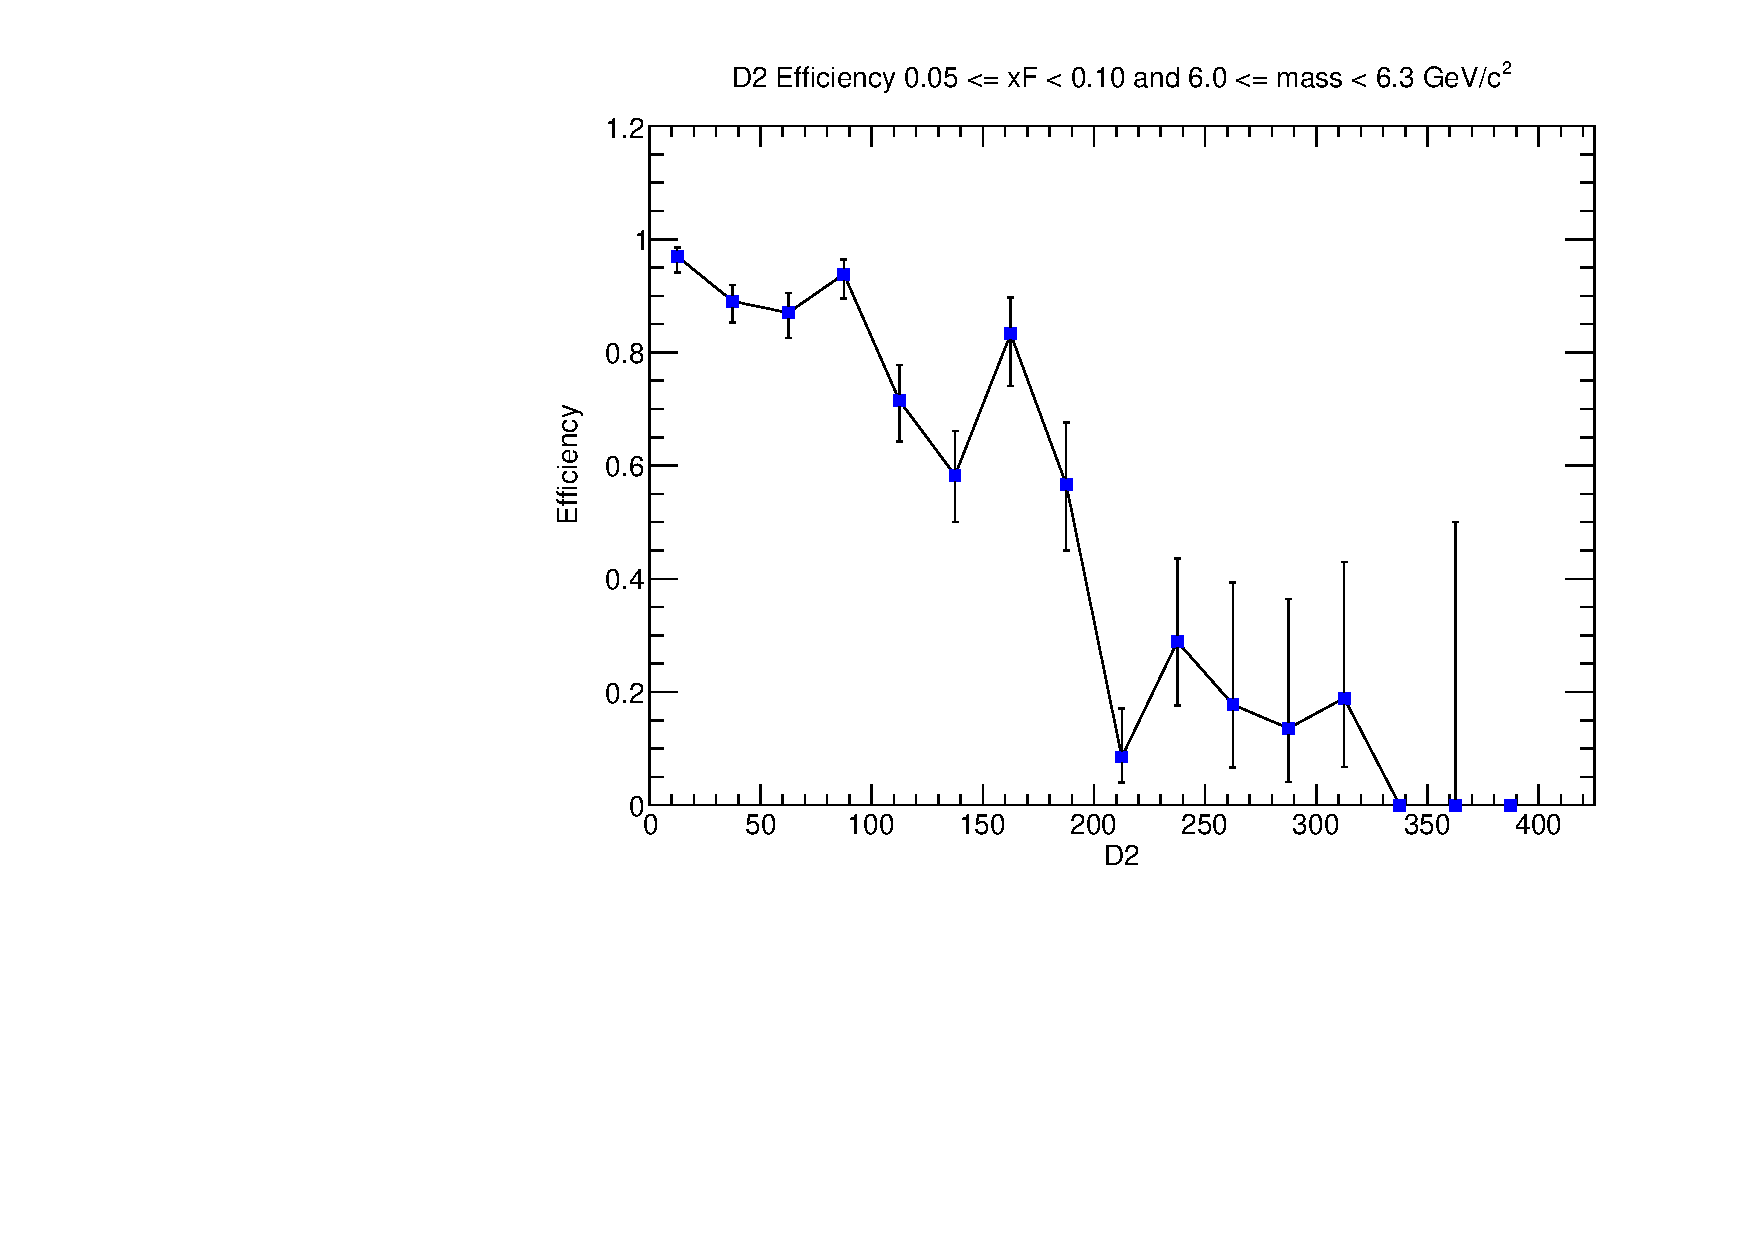
\includegraphics[width=\textwidth]{./kTrackerEfficiencyPlots/D2_Efficiency_xF1_mass6.pdf}
        \caption{$6.0 \leq m < 6.3$ GeV/$c^2$}
        \label{fig:xF1_mass6}
    \end{subfigure}
    \hfill
    \begin{subfigure}[b]{0.32\textwidth}
        \centering
        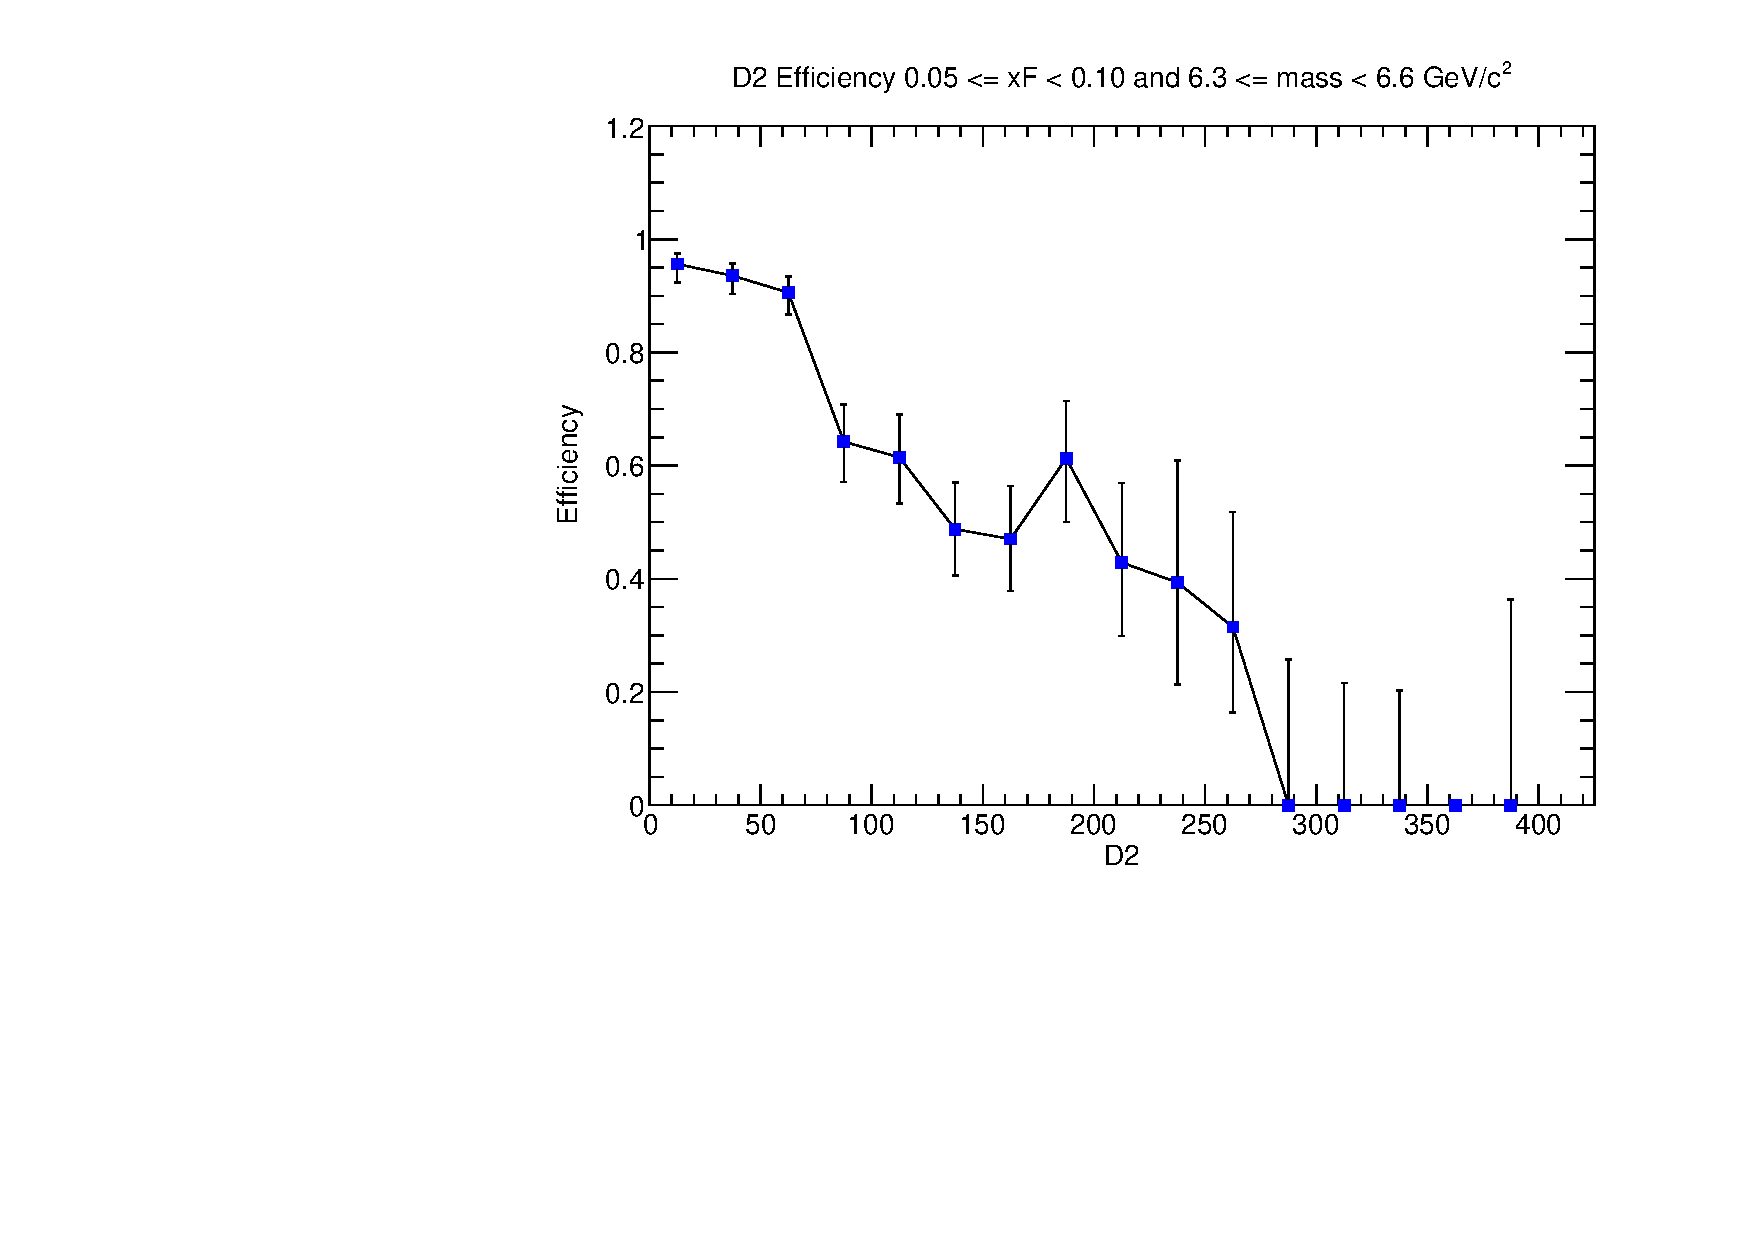
\includegraphics[width=\textwidth]{./kTrackerEfficiencyPlots/D2_Efficiency_xF1_mass7.pdf}
        \caption{$6.3 \leq m < 6.6$ GeV/$c^2$}
        \label{fig:xF1_mass7}
    \end{subfigure}
    \hfill
    \begin{subfigure}[b]{0.32\textwidth}
        \centering
        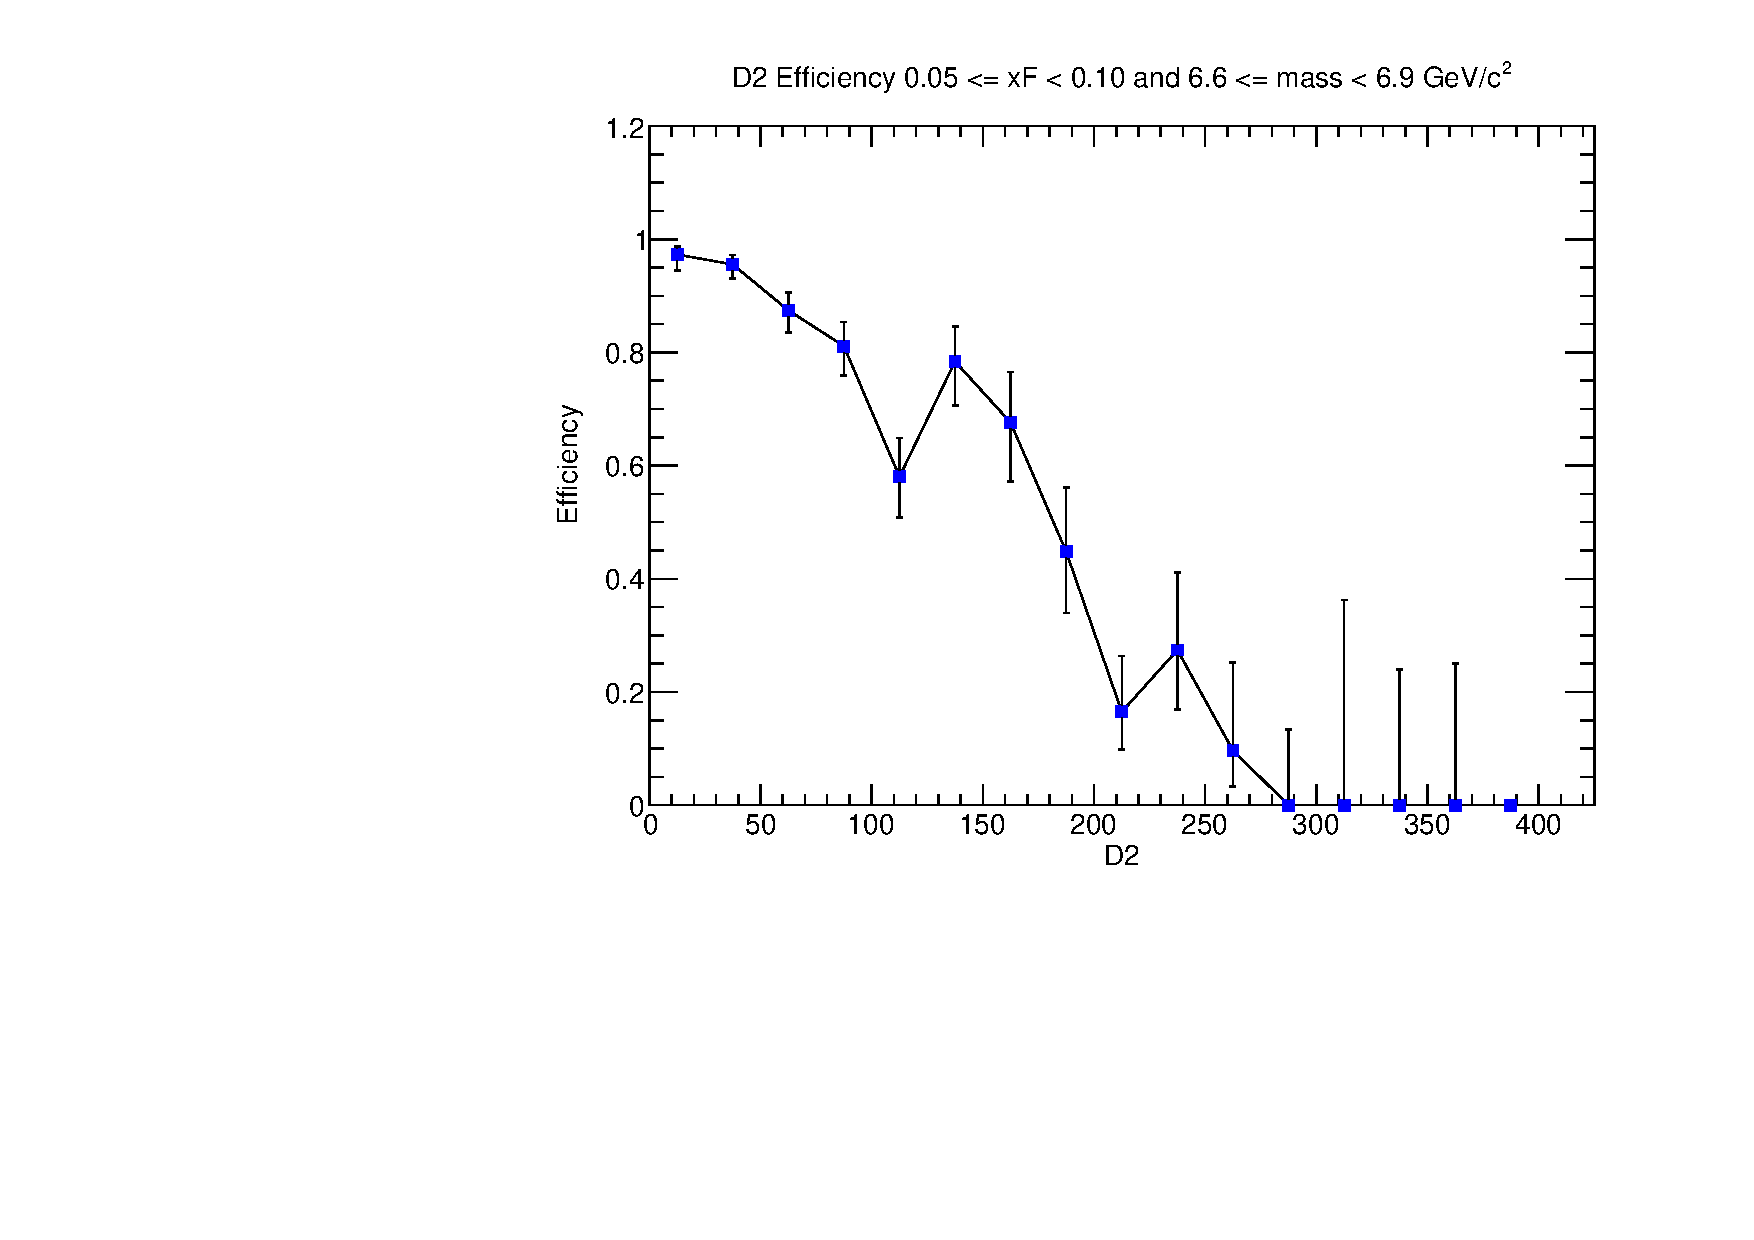
\includegraphics[width=\textwidth]{./kTrackerEfficiencyPlots/D2_Efficiency_xF1_mass8.pdf}
        \caption{$6.6 \leq m < 6.9$ GeV/$c^2$}
        \label{fig:xF1_mass8}
    \end{subfigure}
    \vspace{0.5cm}
    \begin{subfigure}[b]{0.32\textwidth}
        \centering
        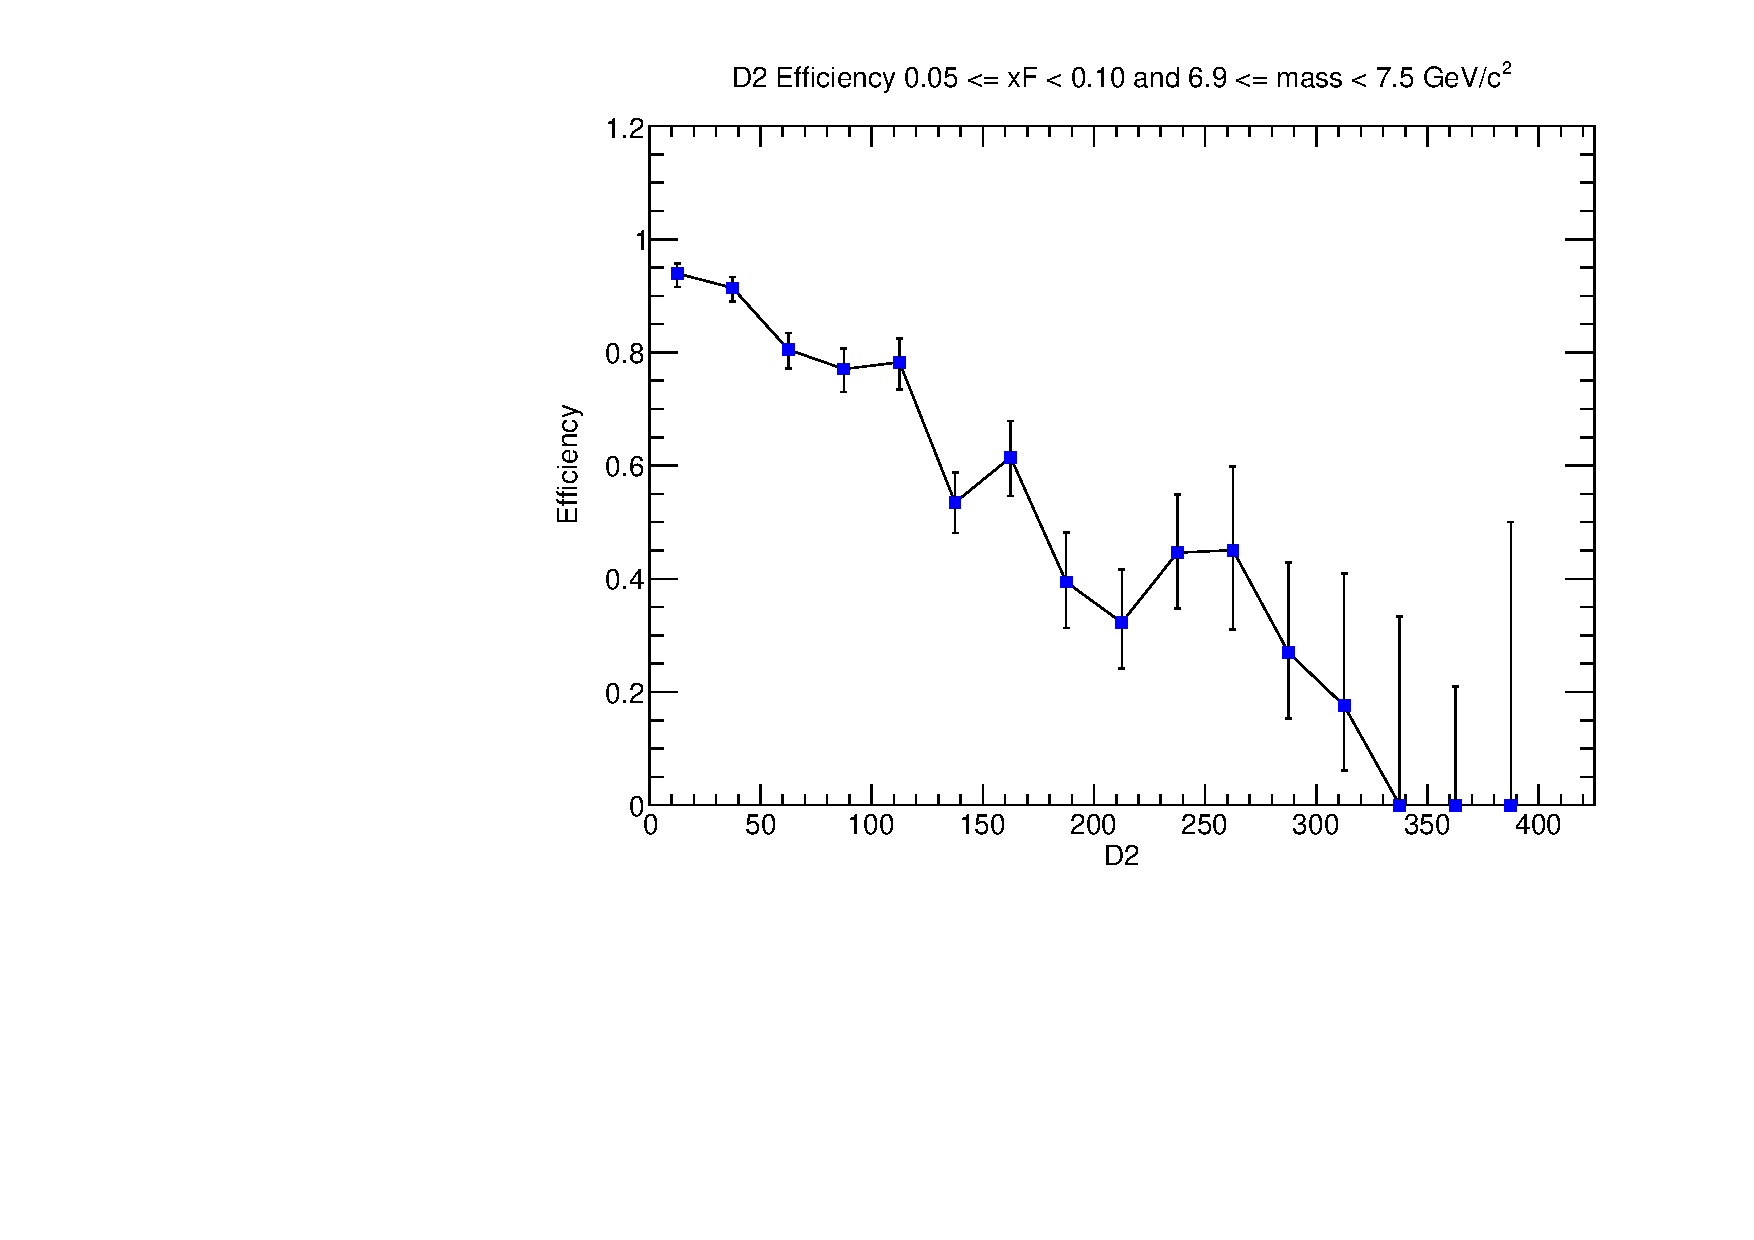
\includegraphics[width=\textwidth]{./kTrackerEfficiencyPlots/D2_Efficiency_xF1_mass9.pdf}
        \caption{$6.9 \leq m < 7.5$ GeV/$c^2$}
        \label{fig:xF1_mass9}
    \end{subfigure}
    \hfill
    \begin{subfigure}[b]{0.32\textwidth}
        \centering
        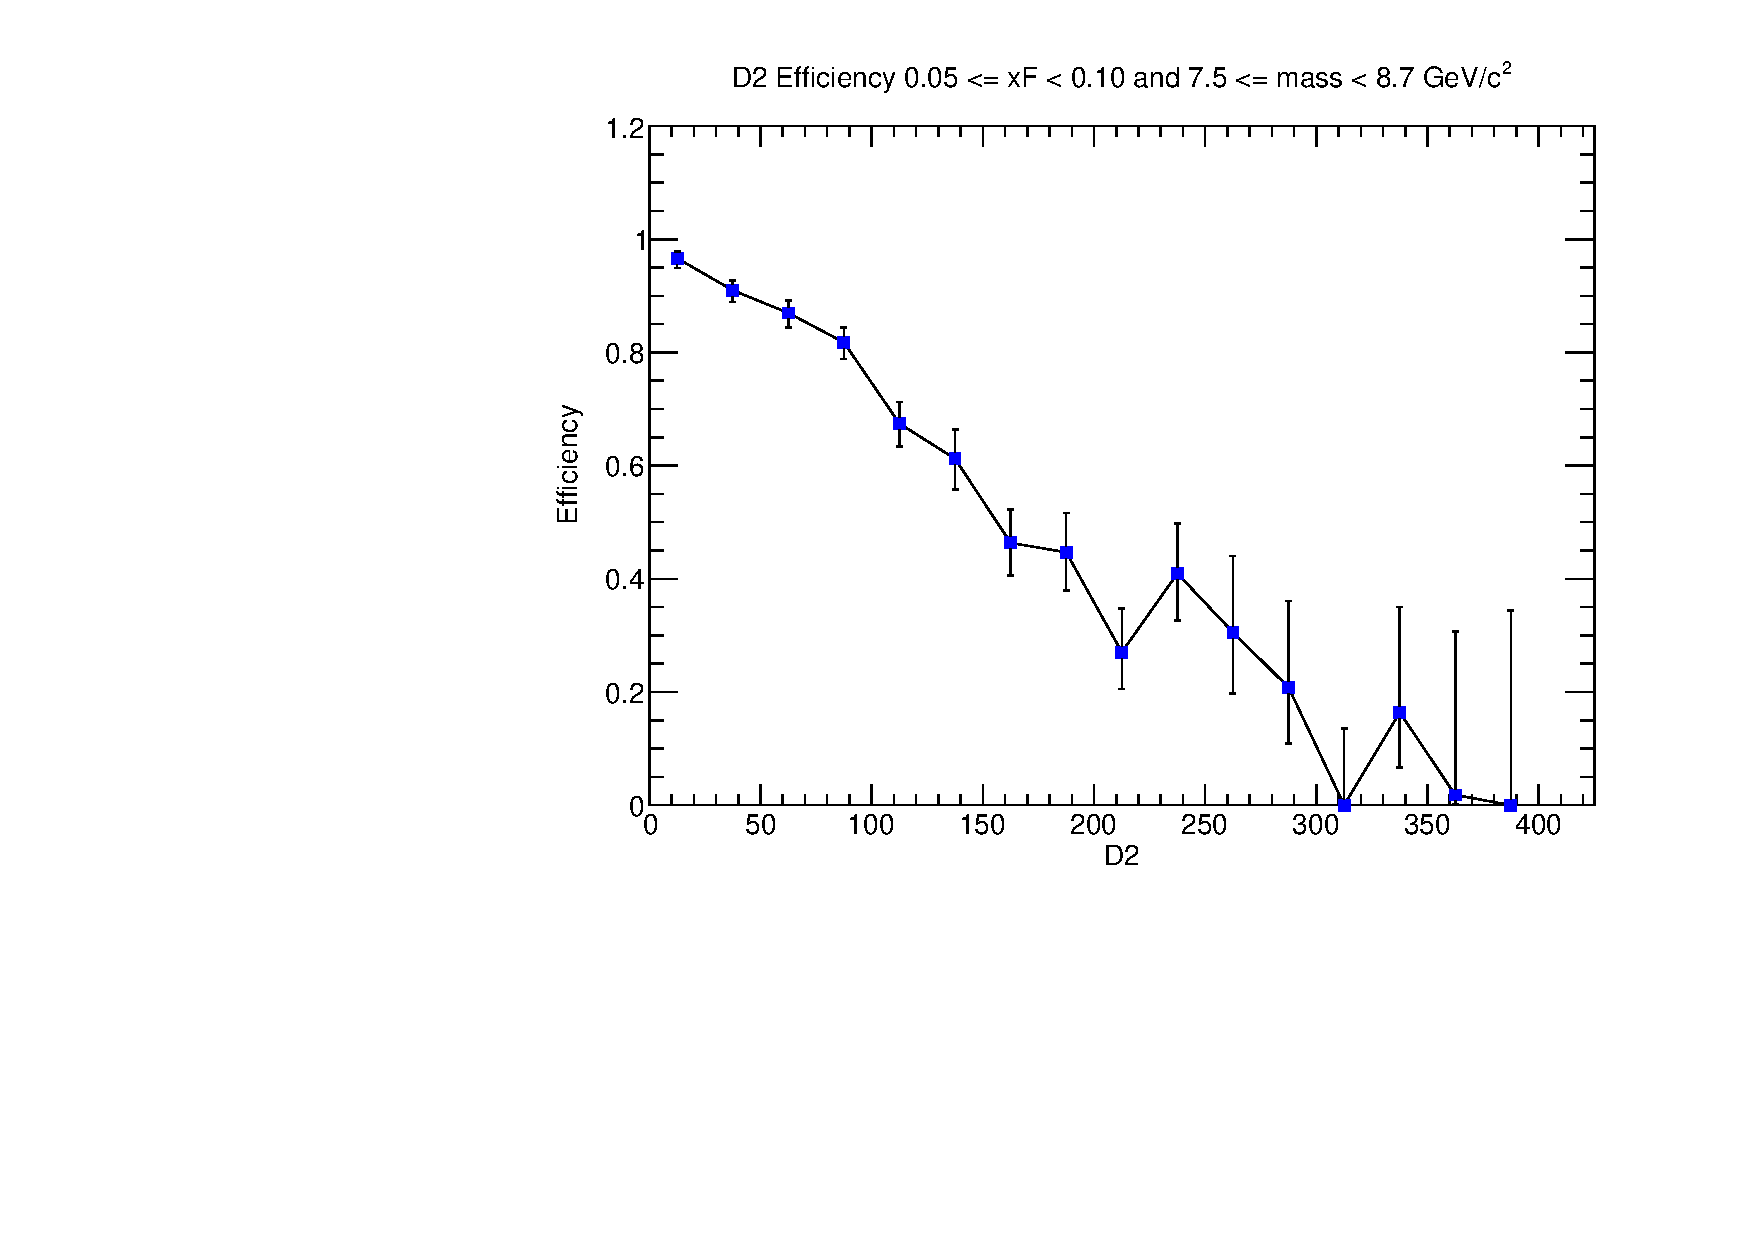
\includegraphics[width=\textwidth]{./kTrackerEfficiencyPlots/D2_Efficiency_xF1_mass10.pdf}
        \caption{$7.5 \leq m < 8.7$ GeV/$c^2$}
        \label{fig:xF1_mass10}
    \end{subfigure}
    \hfill
    \caption{Efficiency plots for the $x_F$ bin $0.05 \leq x_F < 0.10$.}
    \label{fig:xF1}
\end{figure}

\clearpage

\begin{figure}[p]
    \centering
    \begin{subfigure}[b]{0.32\textwidth}
        \centering
        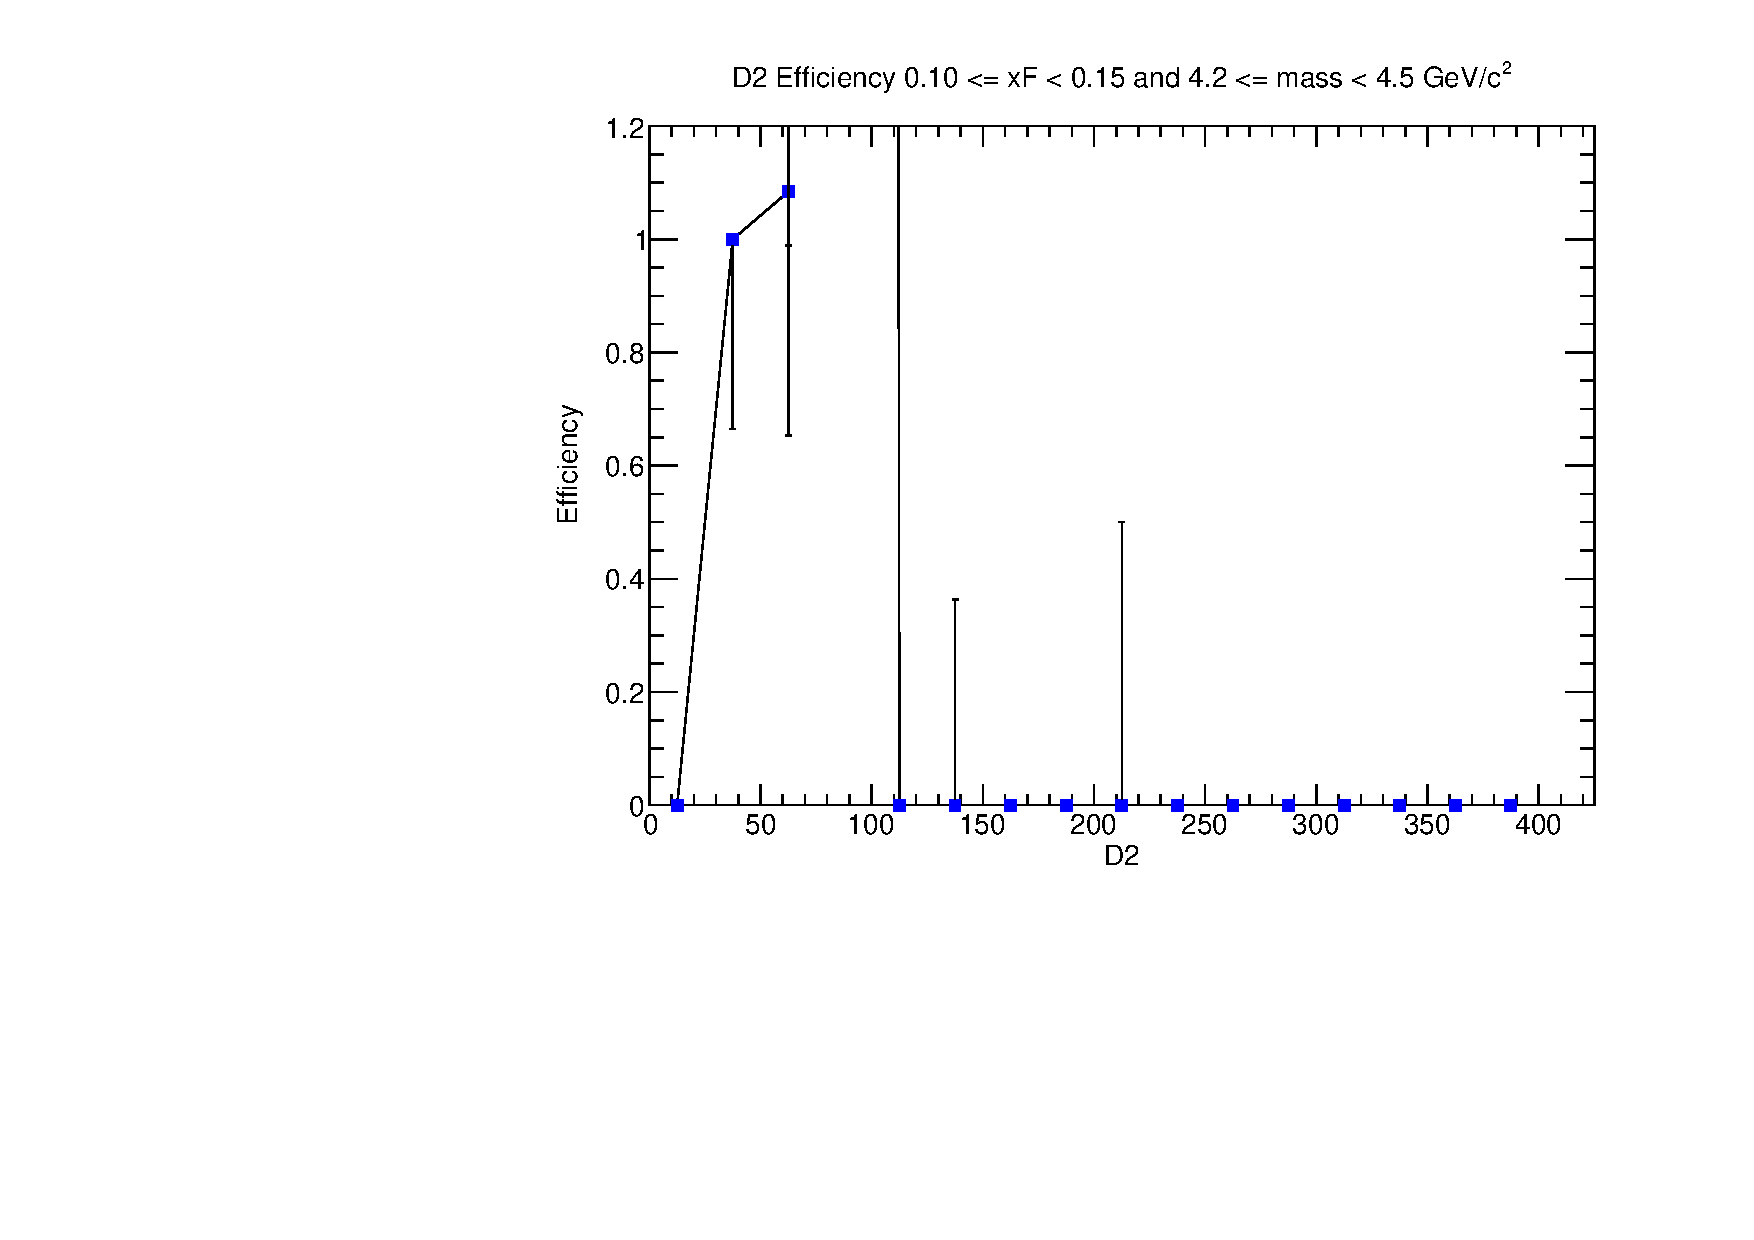
\includegraphics[width=\textwidth]{./kTrackerEfficiencyPlots/D2_Efficiency_xF2_mass0.pdf}
        \caption{$4.2 \leq m < 4.5$ GeV/$c^2$}
        \label{fig:xF2_mass0}
    \end{subfigure}
    \hfill
    \begin{subfigure}[b]{0.32\textwidth}
        \centering
        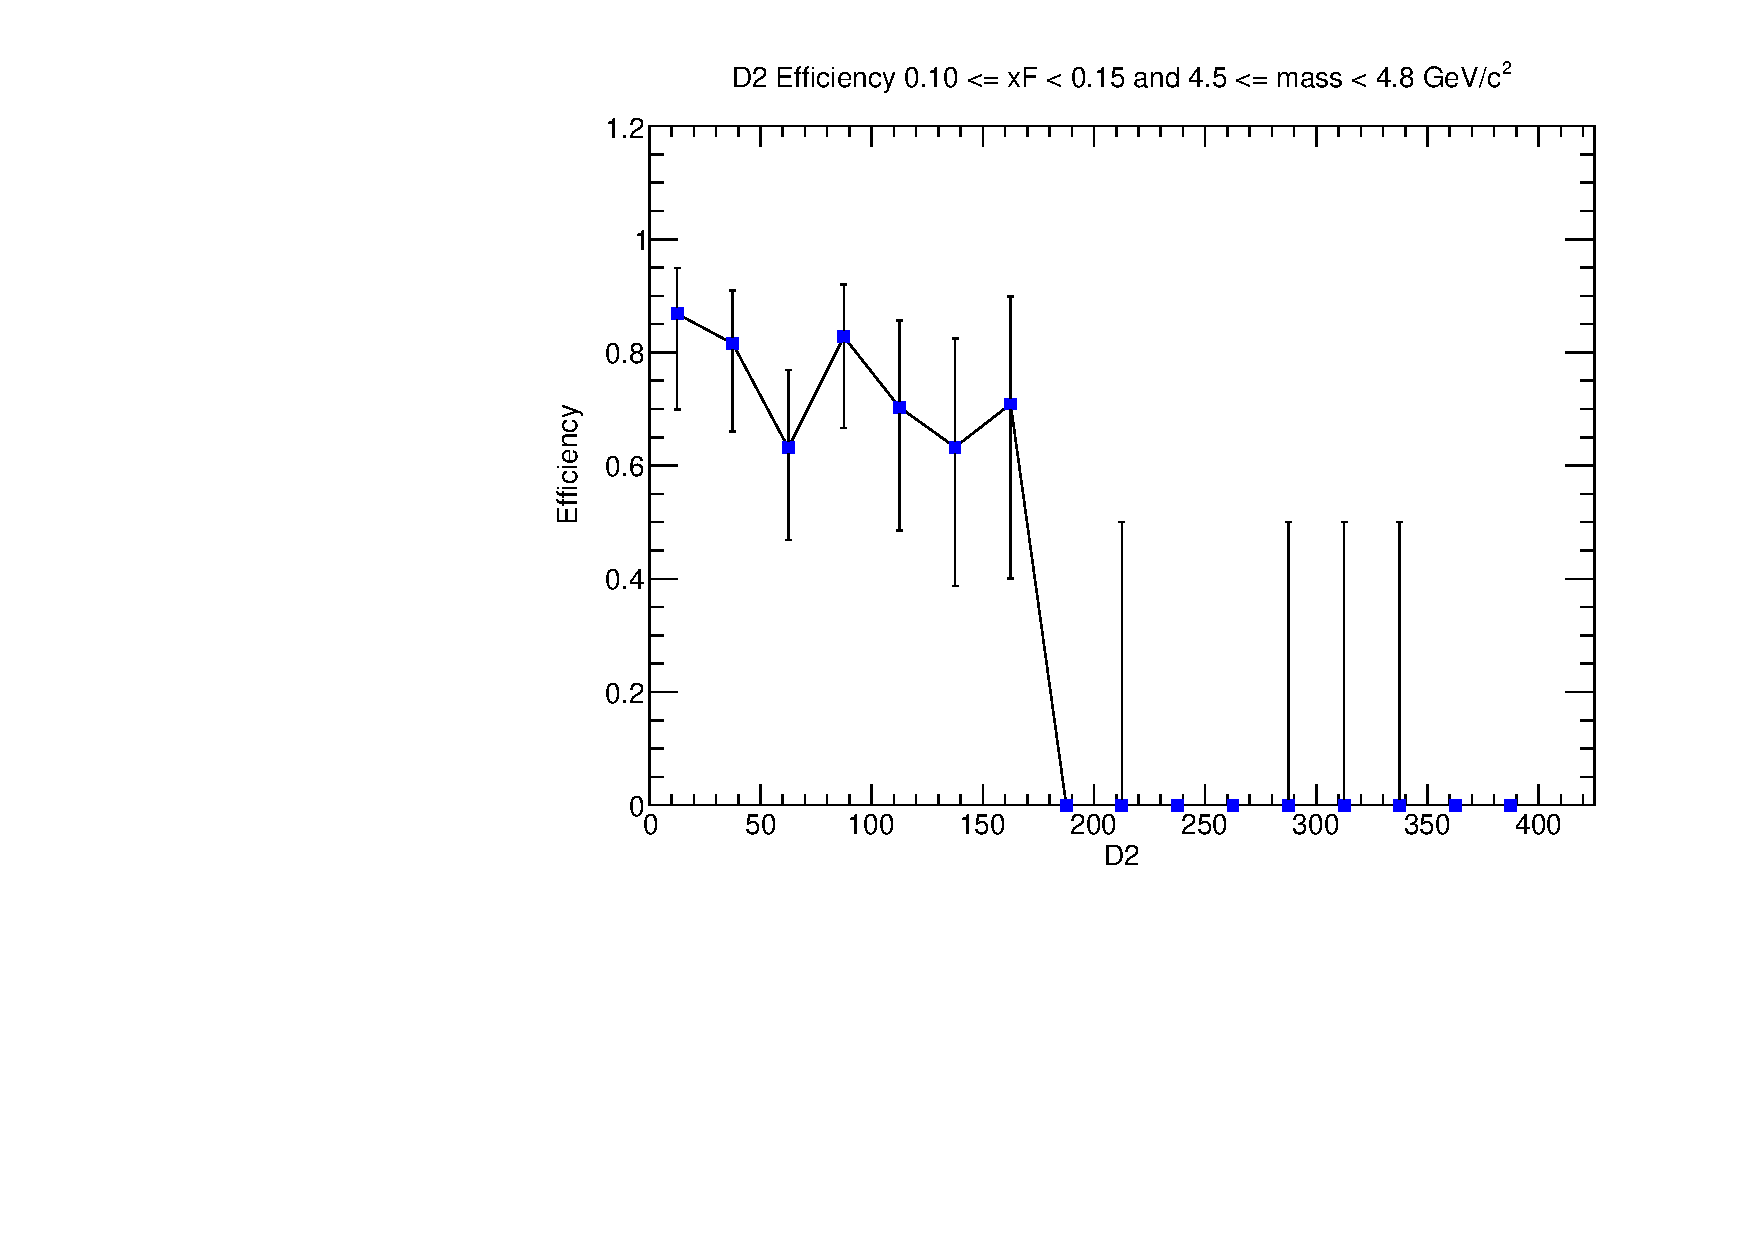
\includegraphics[width=\textwidth]{./kTrackerEfficiencyPlots/D2_Efficiency_xF2_mass1.pdf}
        \caption{$4.5 \leq m < 4.8$ GeV/$c^2$}
        \label{fig:xF2_mass1}
    \end{subfigure}
    \hfill
    \begin{subfigure}[b]{0.32\textwidth}
        \centering
        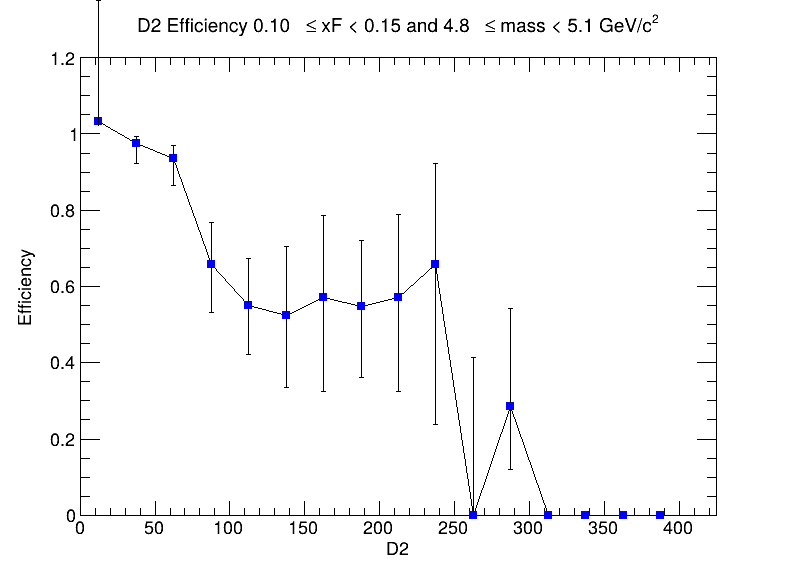
\includegraphics[width=\textwidth]{./kTrackerEfficiencyPlots/D2_Efficiency_xF2_mass2.png}
        \caption{$4.8 \leq m < 5.1$ GeV/$c^2$}
        \label{fig:xF2_mass2}
    \end{subfigure}
    \vspace{0.5cm}
    \begin{subfigure}[b]{0.32\textwidth}
        \centering
        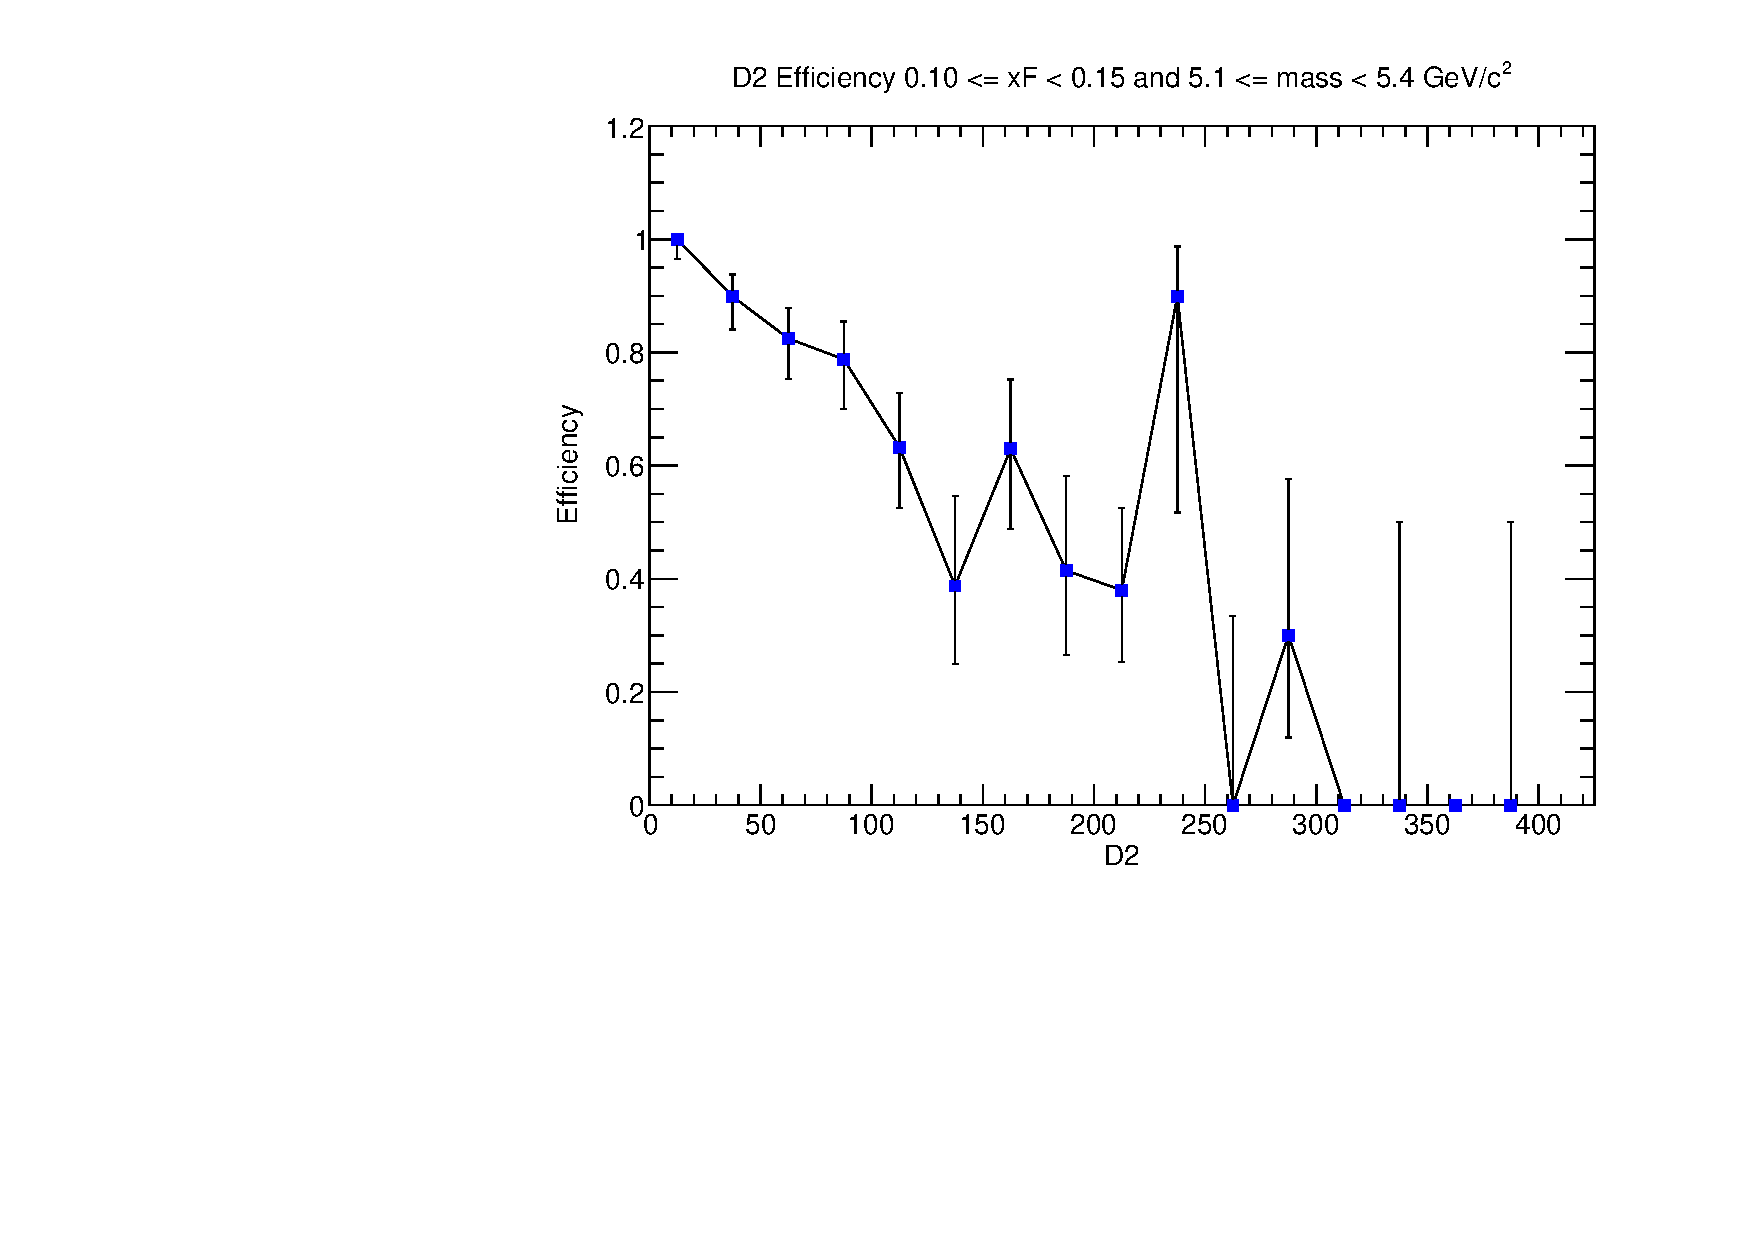
\includegraphics[width=\textwidth]{./kTrackerEfficiencyPlots/D2_Efficiency_xF2_mass3.pdf}
        \caption{$5.1 \leq m < 5.4$ GeV/$c^2$}
        \label{fig:xF2_mass3}
    \end{subfigure}
    \hfill
    \begin{subfigure}[b]{0.32\textwidth}
        \centering
        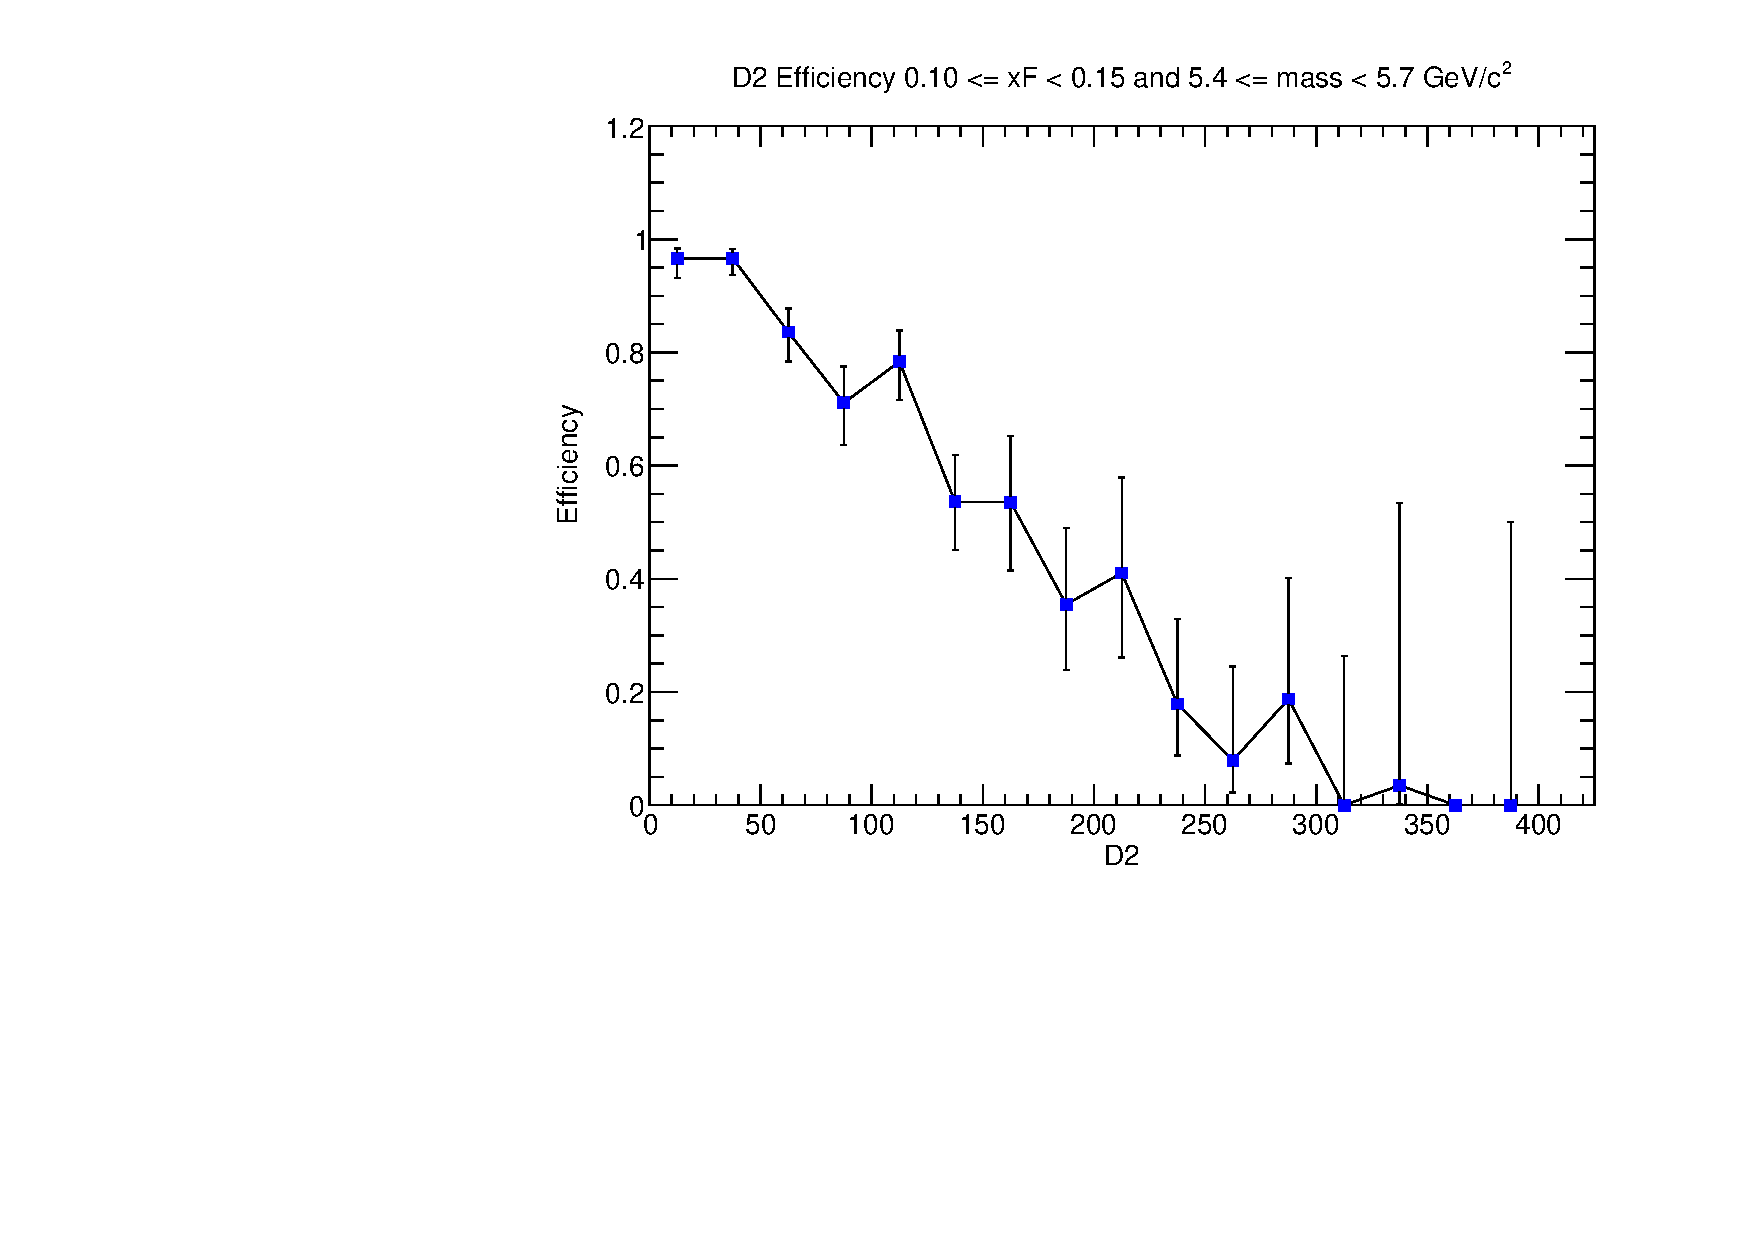
\includegraphics[width=\textwidth]{./kTrackerEfficiencyPlots/D2_Efficiency_xF2_mass4.pdf}
        \caption{$5.4 \leq m < 5.7$ GeV/$c^2$}
        \label{fig:xF2_mass4}
    \end{subfigure}
    \hfill
    \begin{subfigure}[b]{0.32\textwidth}
        \centering
        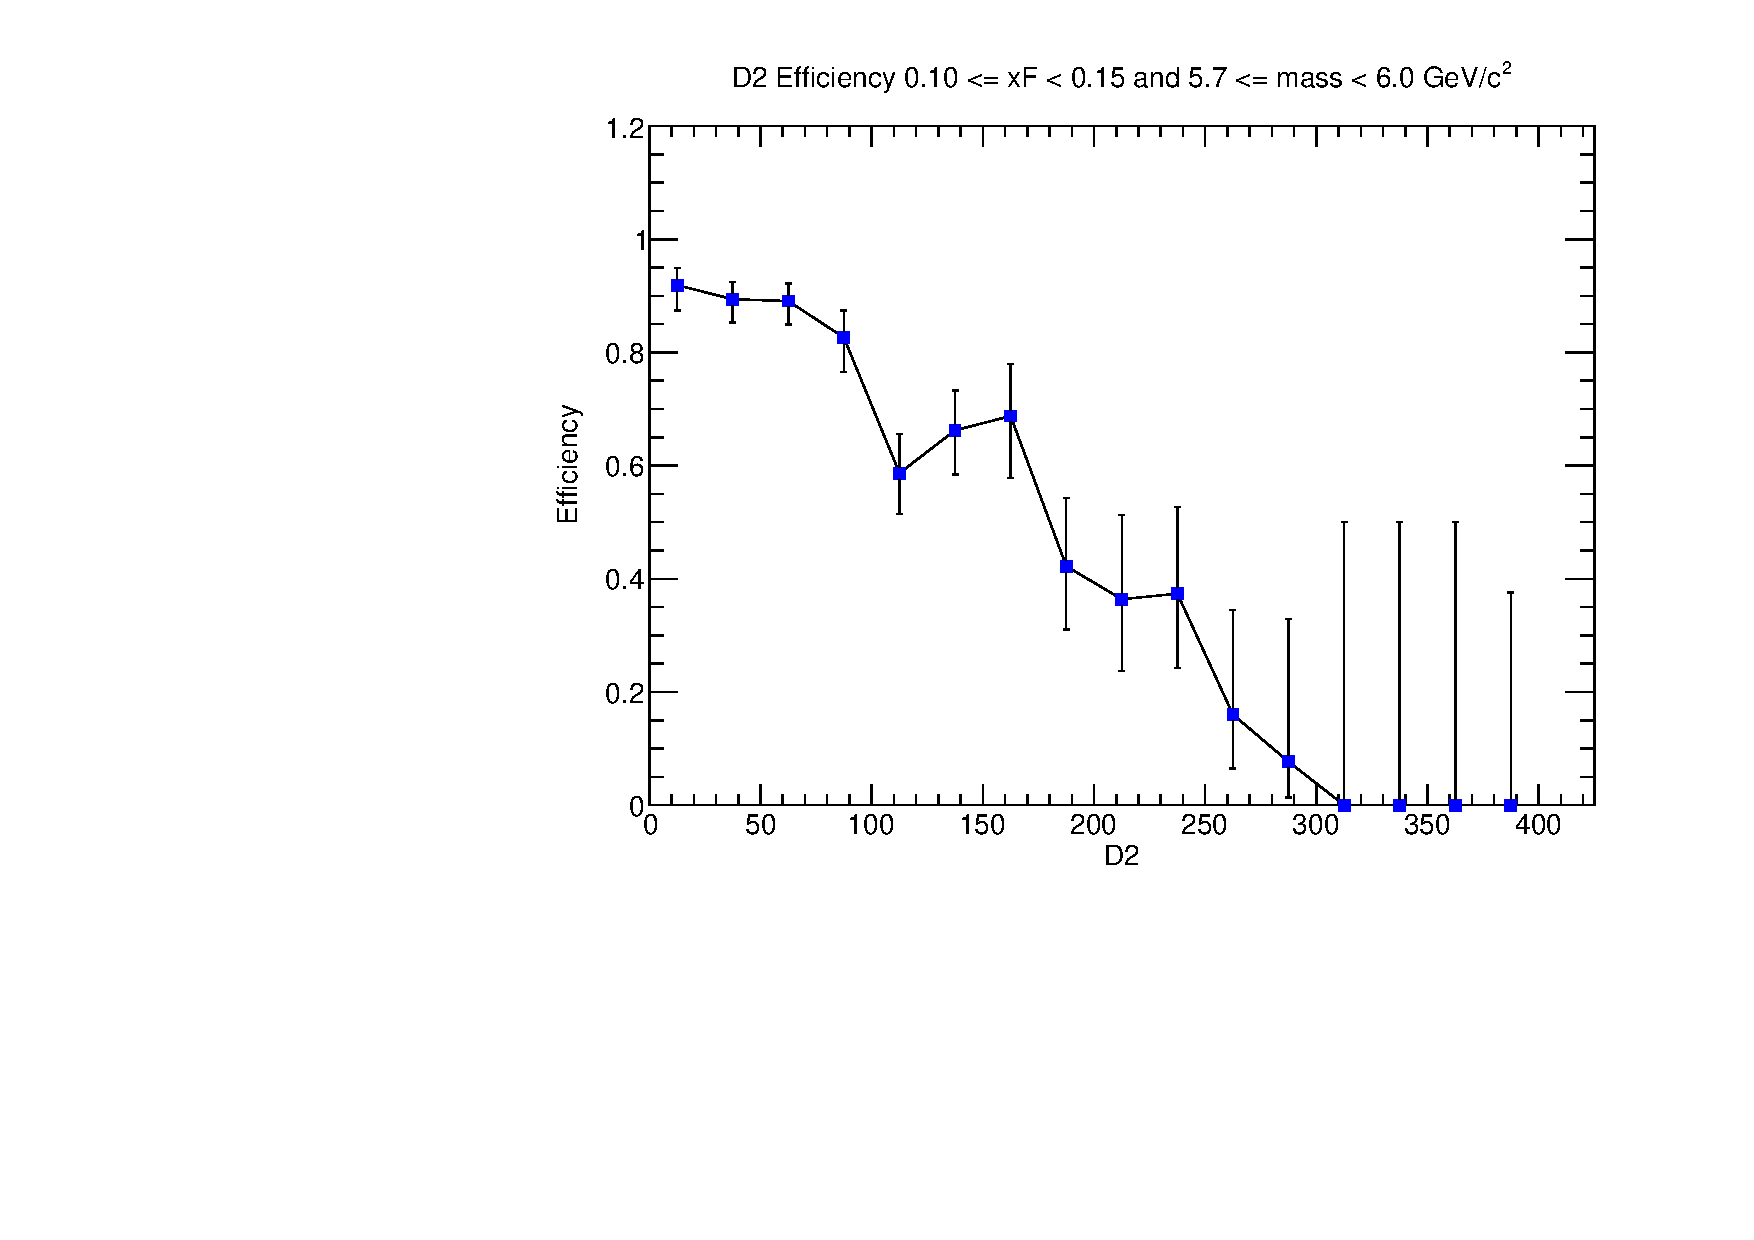
\includegraphics[width=\textwidth]{./kTrackerEfficiencyPlots/D2_Efficiency_xF2_mass5.pdf}
        \caption{$5.7 \leq m < 6.0$ GeV/$c^2$}
        \label{fig:xF2_mass5}
    \end{subfigure}
    \vspace{0.5cm}
    \begin{subfigure}[b]{0.32\textwidth}
        \centering
        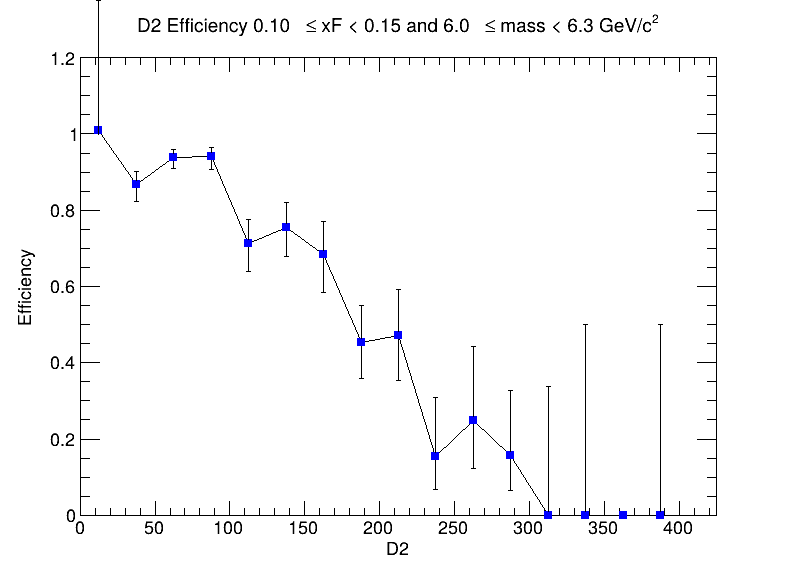
\includegraphics[width=\textwidth]{./kTrackerEfficiencyPlots/D2_Efficiency_xF2_mass6.png}
        \caption{$6.0 \leq m < 6.3$ GeV/$c^2$}
        \label{fig:xF2_mass6}
    \end{subfigure}
    \hfill
    \begin{subfigure}[b]{0.32\textwidth}
        \centering
        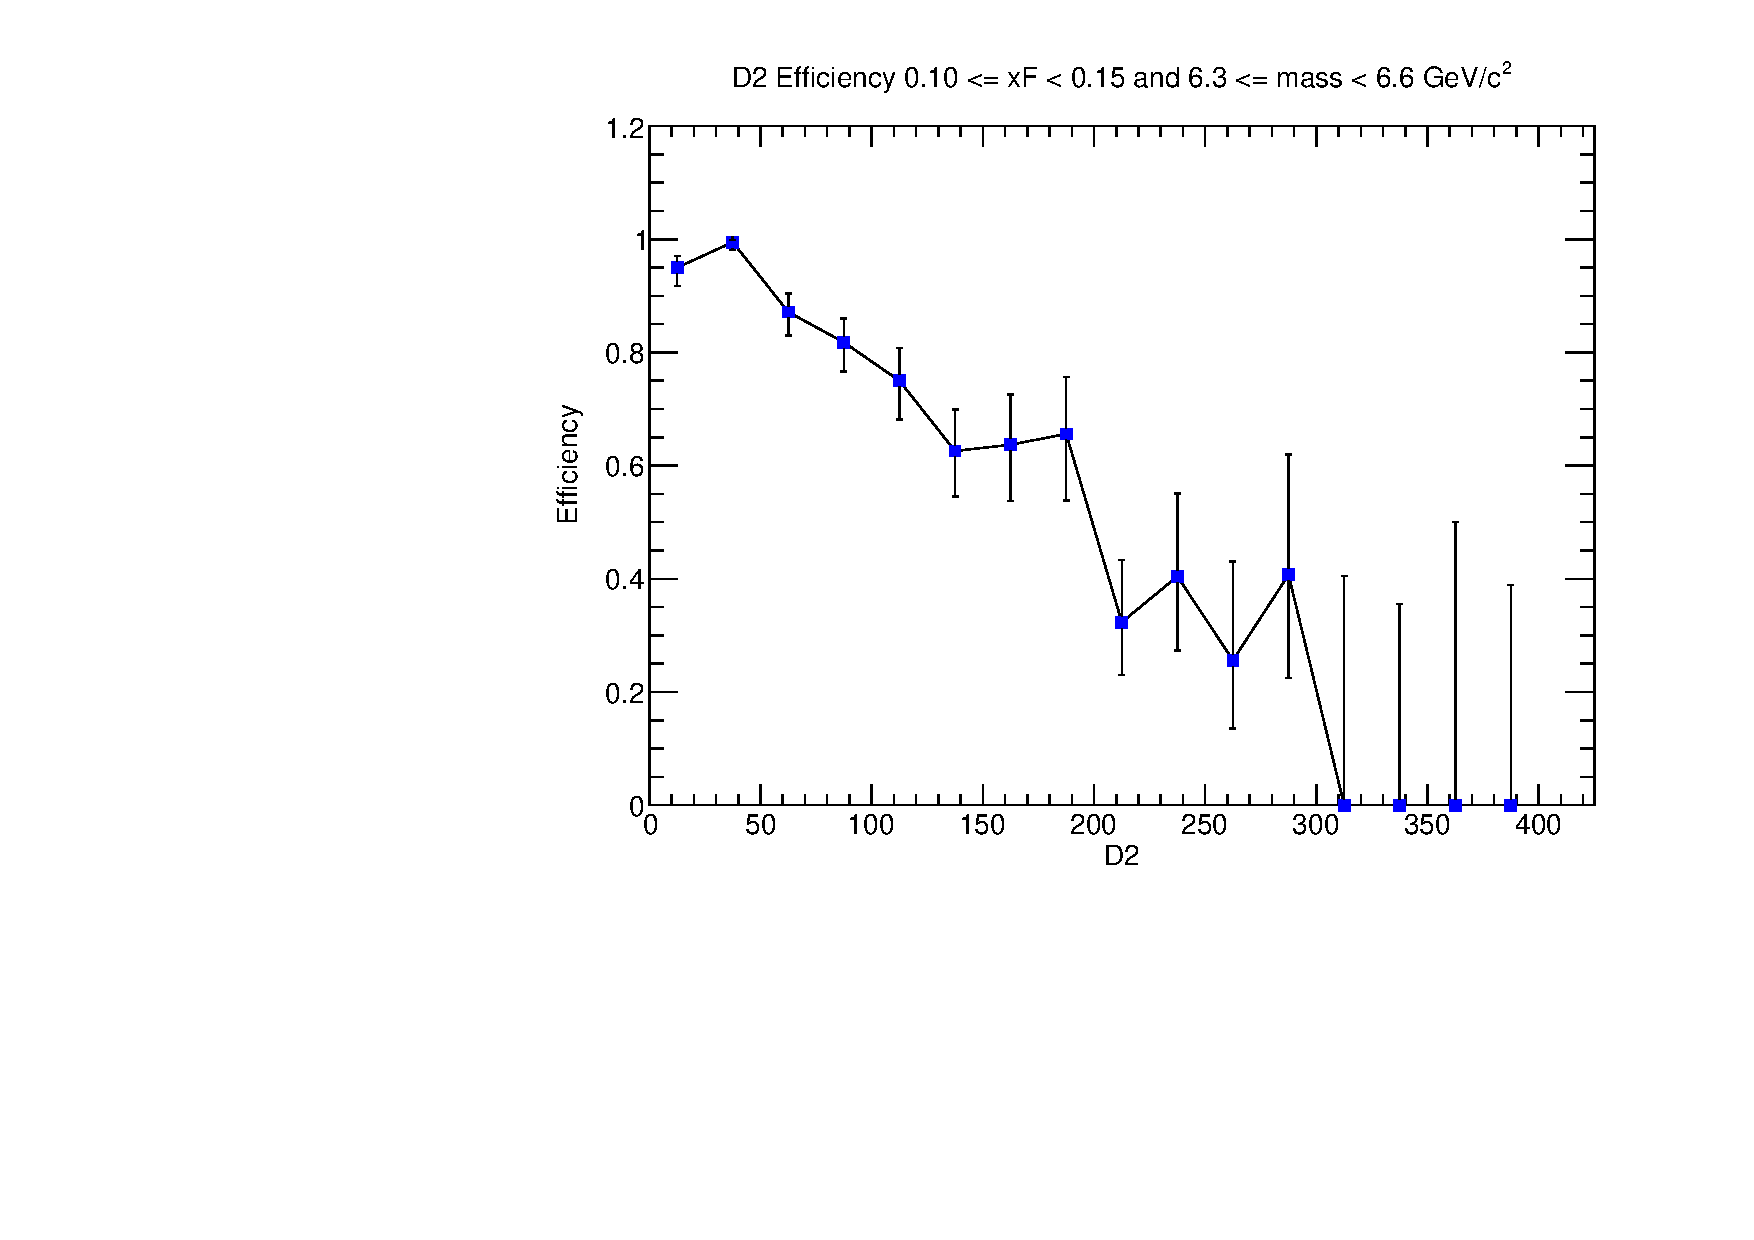
\includegraphics[width=\textwidth]{./kTrackerEfficiencyPlots/D2_Efficiency_xF2_mass7.pdf}
        \caption{$6.3 \leq m < 6.6$ GeV/$c^2$}
        \label{fig:xF2_mass7}
    \end{subfigure}
    \hfill
    \begin{subfigure}[b]{0.32\textwidth}
        \centering
        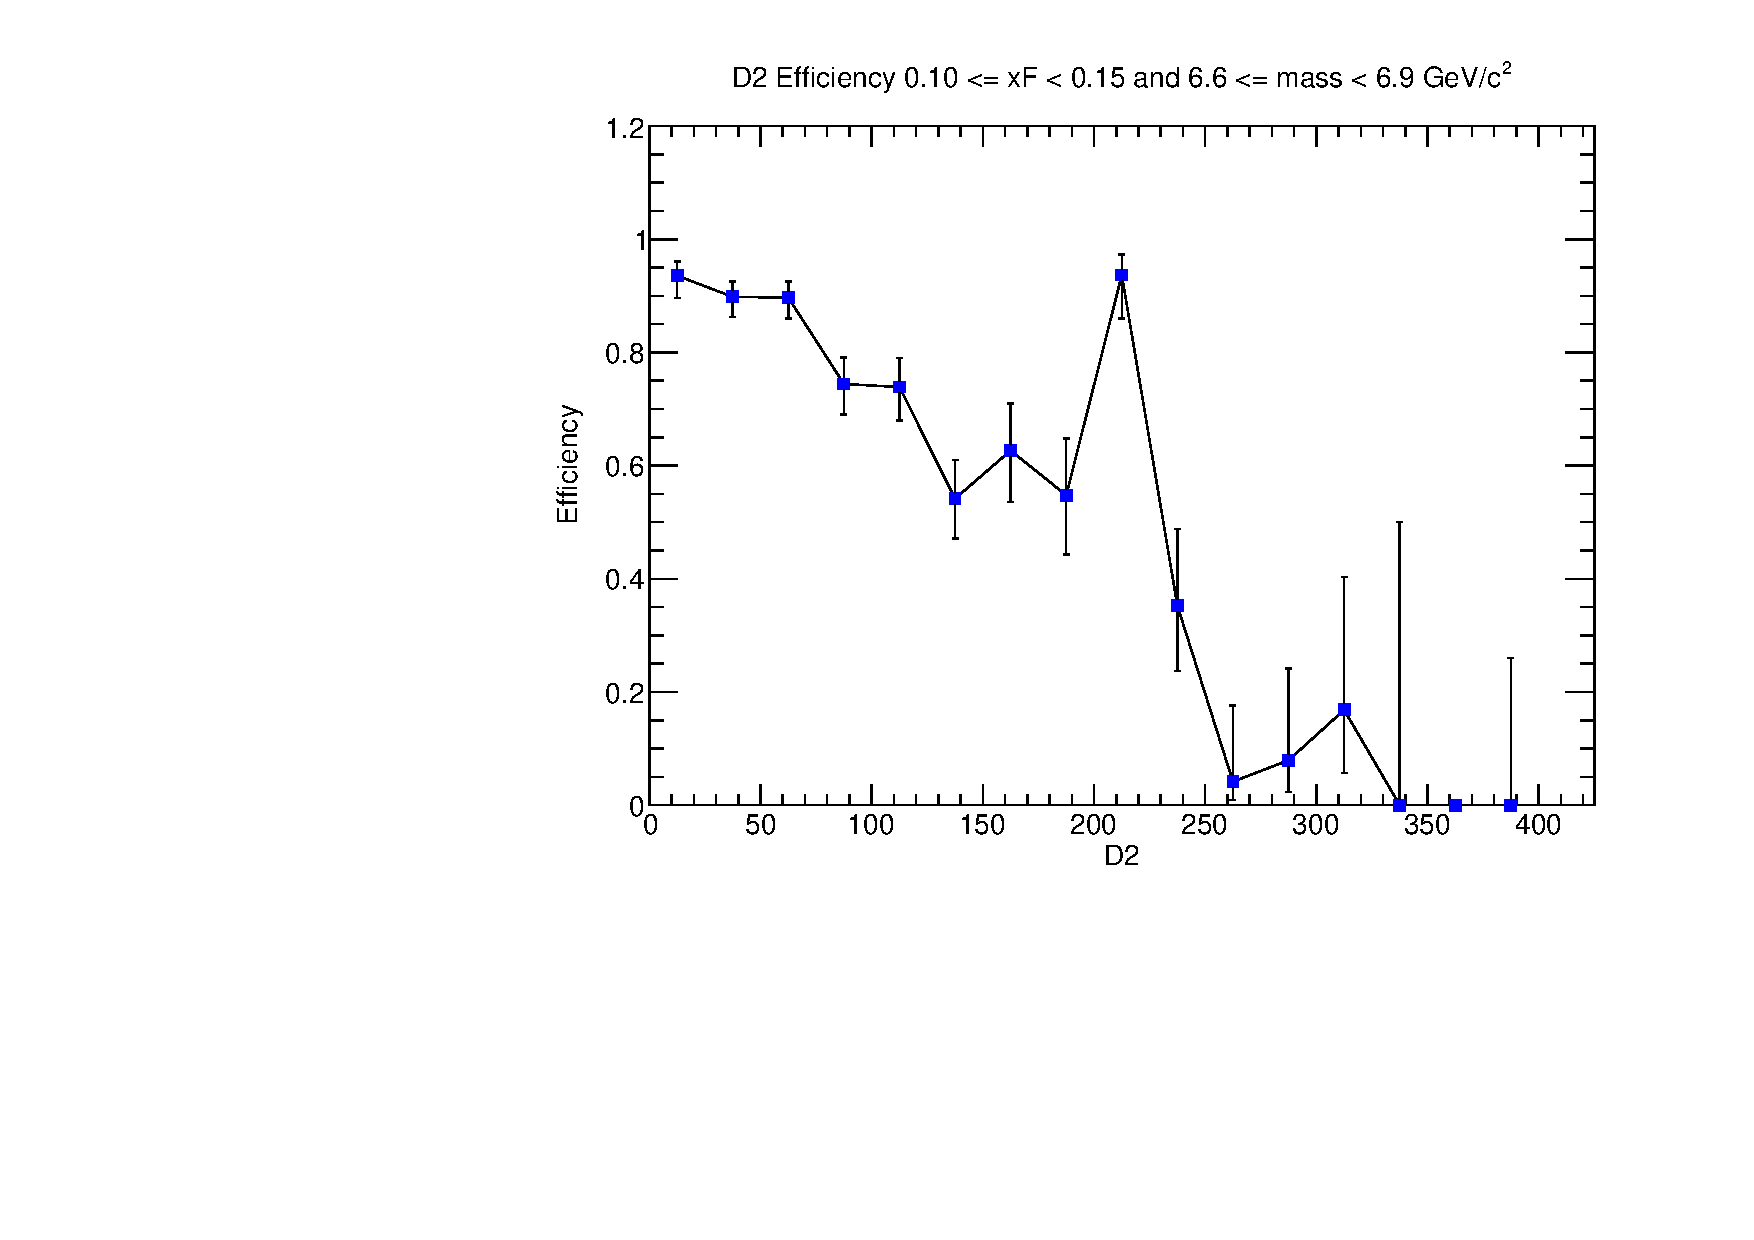
\includegraphics[width=\textwidth]{./kTrackerEfficiencyPlots/D2_Efficiency_xF2_mass8.pdf}
        \caption{$6.6 \leq m < 6.9$ GeV/$c^2$}
        \label{fig:xF2_mass8}
    \end{subfigure}
    \vspace{0.5cm}
    \begin{subfigure}[b]{0.32\textwidth}
        \centering
        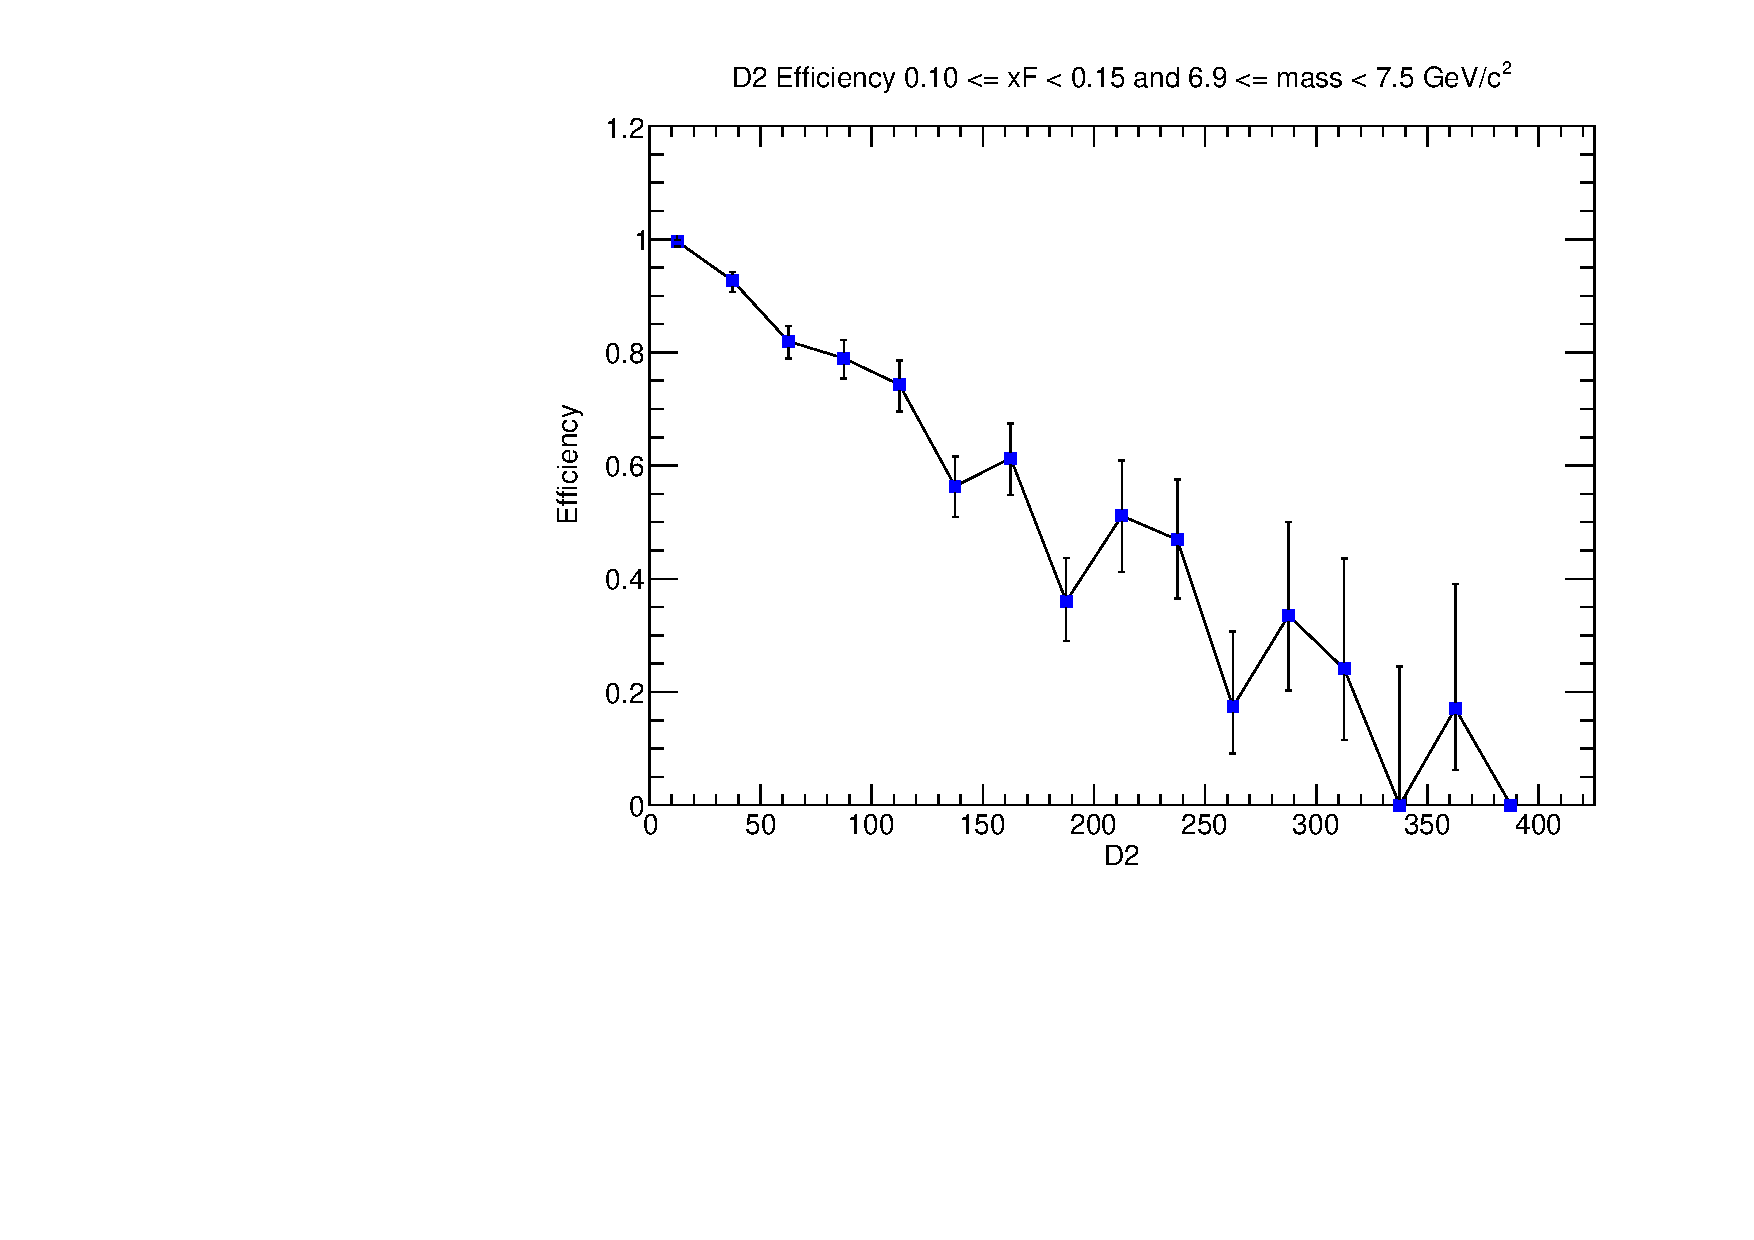
\includegraphics[width=\textwidth]{./kTrackerEfficiencyPlots/D2_Efficiency_xF2_mass9.pdf}
        \caption{$6.9 \leq m < 7.5$ GeV/$c^2$}
        \label{fig:xF2_mass9}
    \end{subfigure}
    \hfill
    \begin{subfigure}[b]{0.32\textwidth}
        \centering
        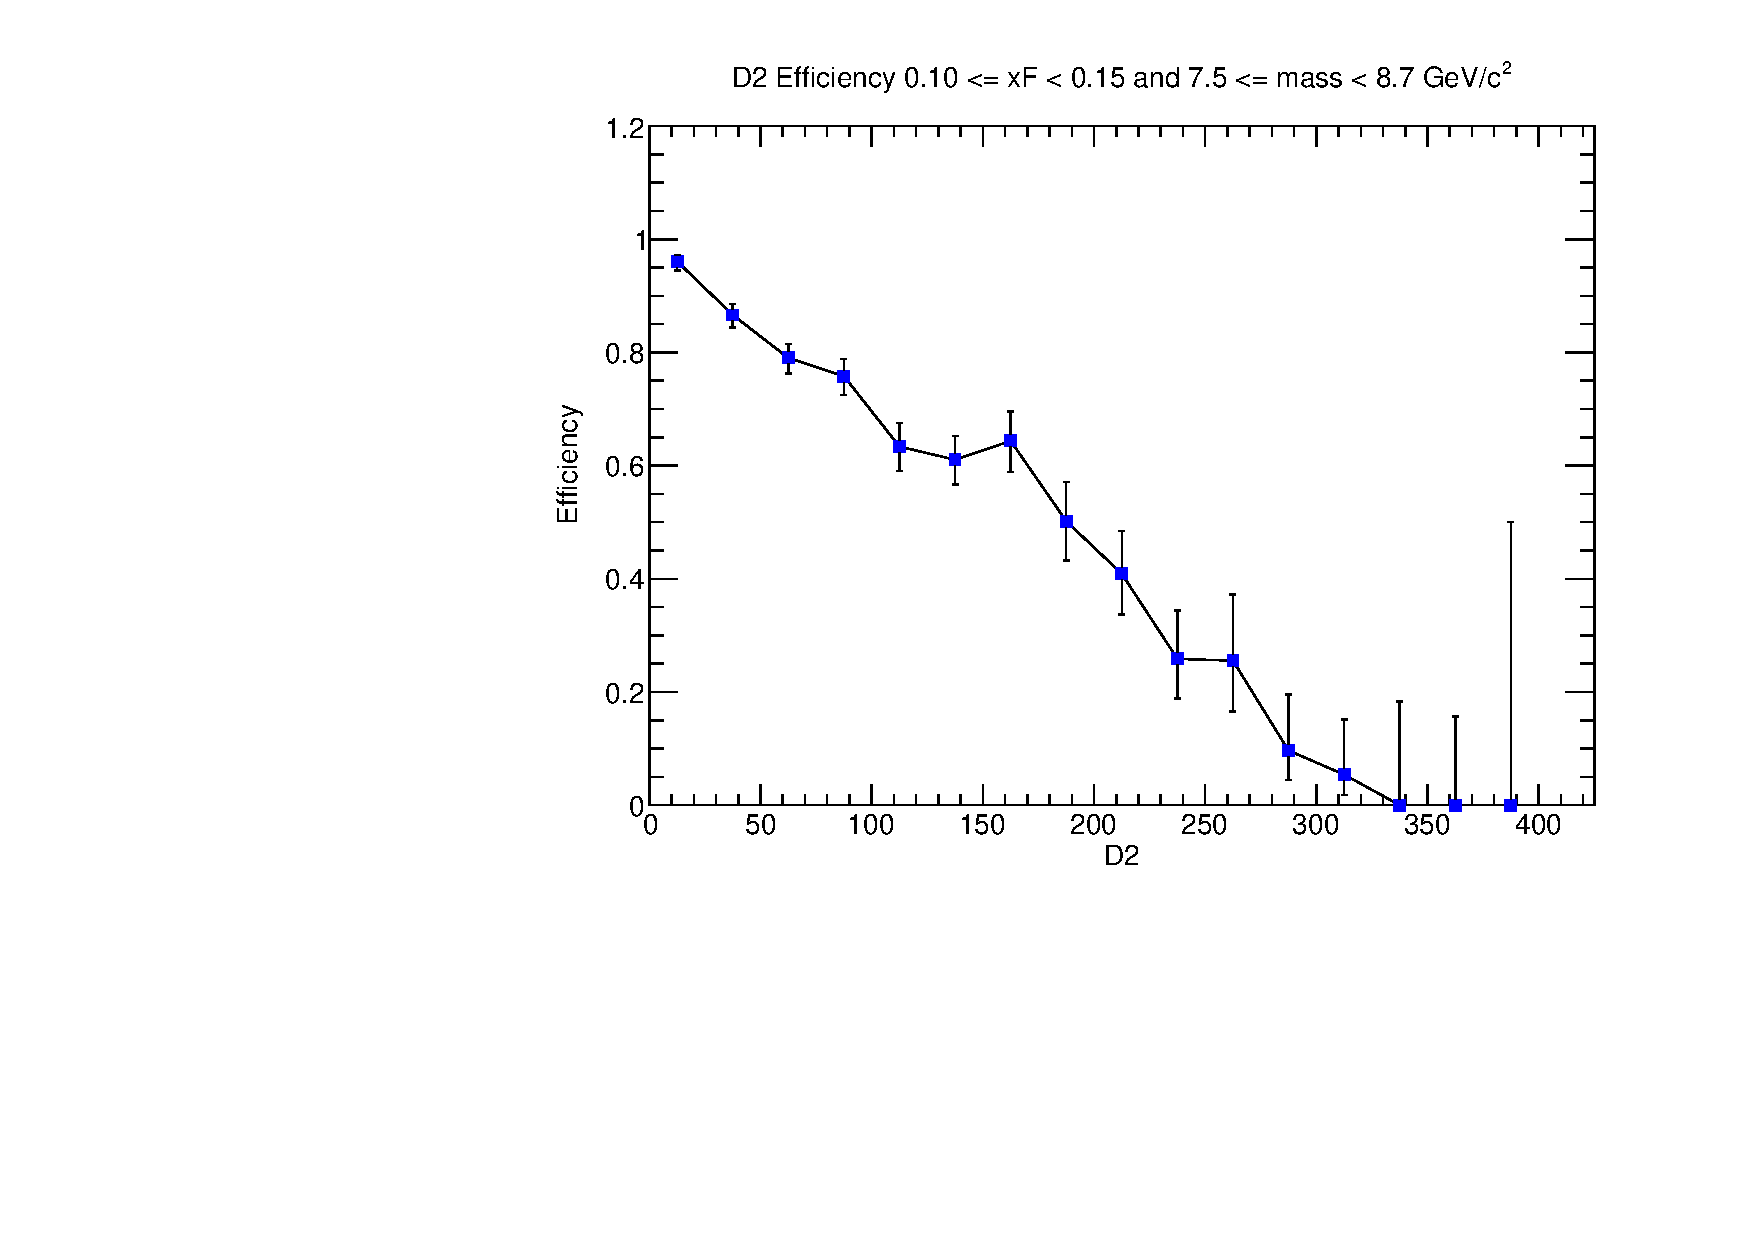
\includegraphics[width=\textwidth]{./kTrackerEfficiencyPlots/D2_Efficiency_xF2_mass10.pdf}
        \caption{$7.5 \leq m < 8.7$ GeV/$c^2$}
        \label{fig:xF2_mass10}
    \end{subfigure}
    \hfill
    \caption{Efficiency plots for the $x_F$ bin $0.10 \leq x_F < 0.15$.}
    \label{fig:xF2}
\end{figure}

\clearpage

\begin{figure}[p]
    \centering
    \begin{subfigure}[b]{0.32\textwidth}
        \centering
        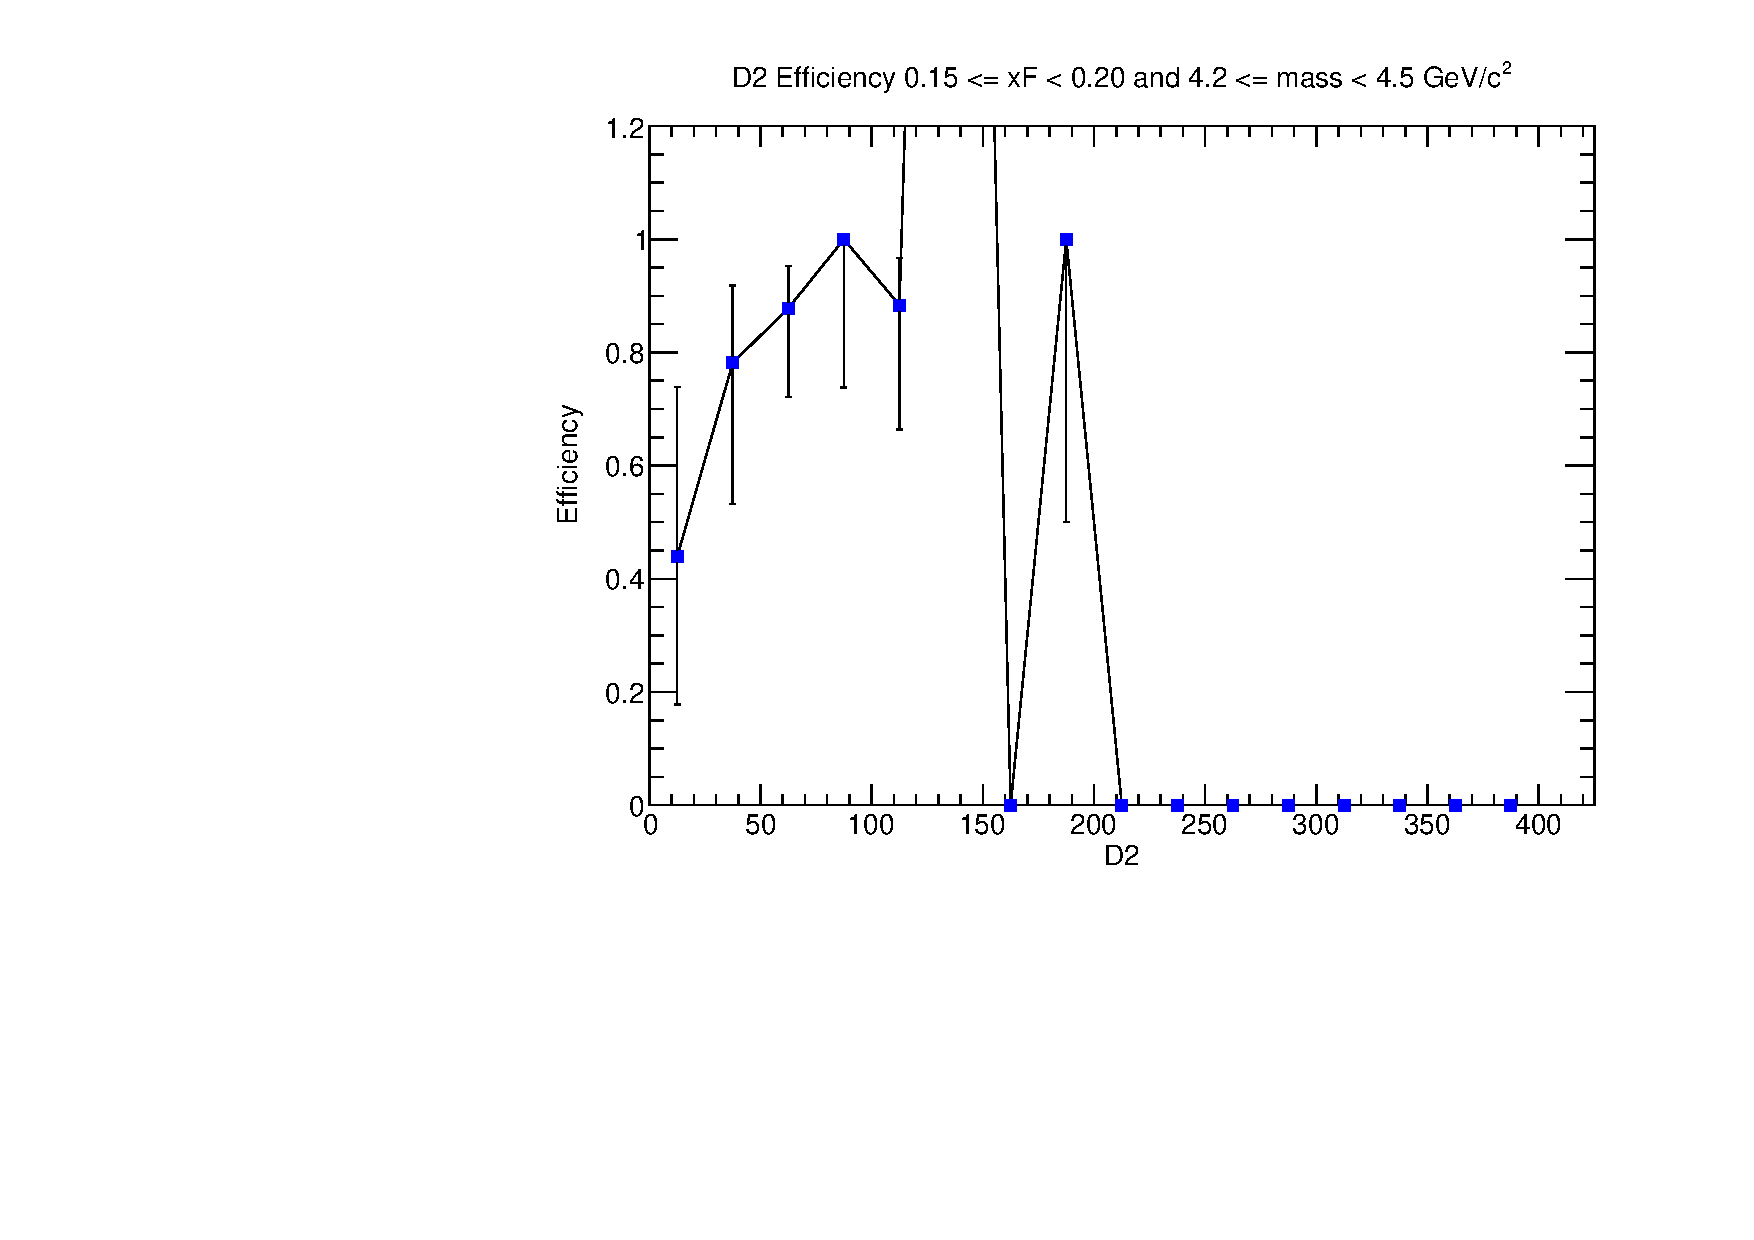
\includegraphics[width=\textwidth]{./kTrackerEfficiencyPlots/D2_Efficiency_xF3_mass0.pdf}
        \caption{$4.2 \leq m < 4.5$ GeV/$c^2$}
        \label{fig:xF3_mass0}
    \end{subfigure}
    \hfill
    \begin{subfigure}[b]{0.32\textwidth}
        \centering
        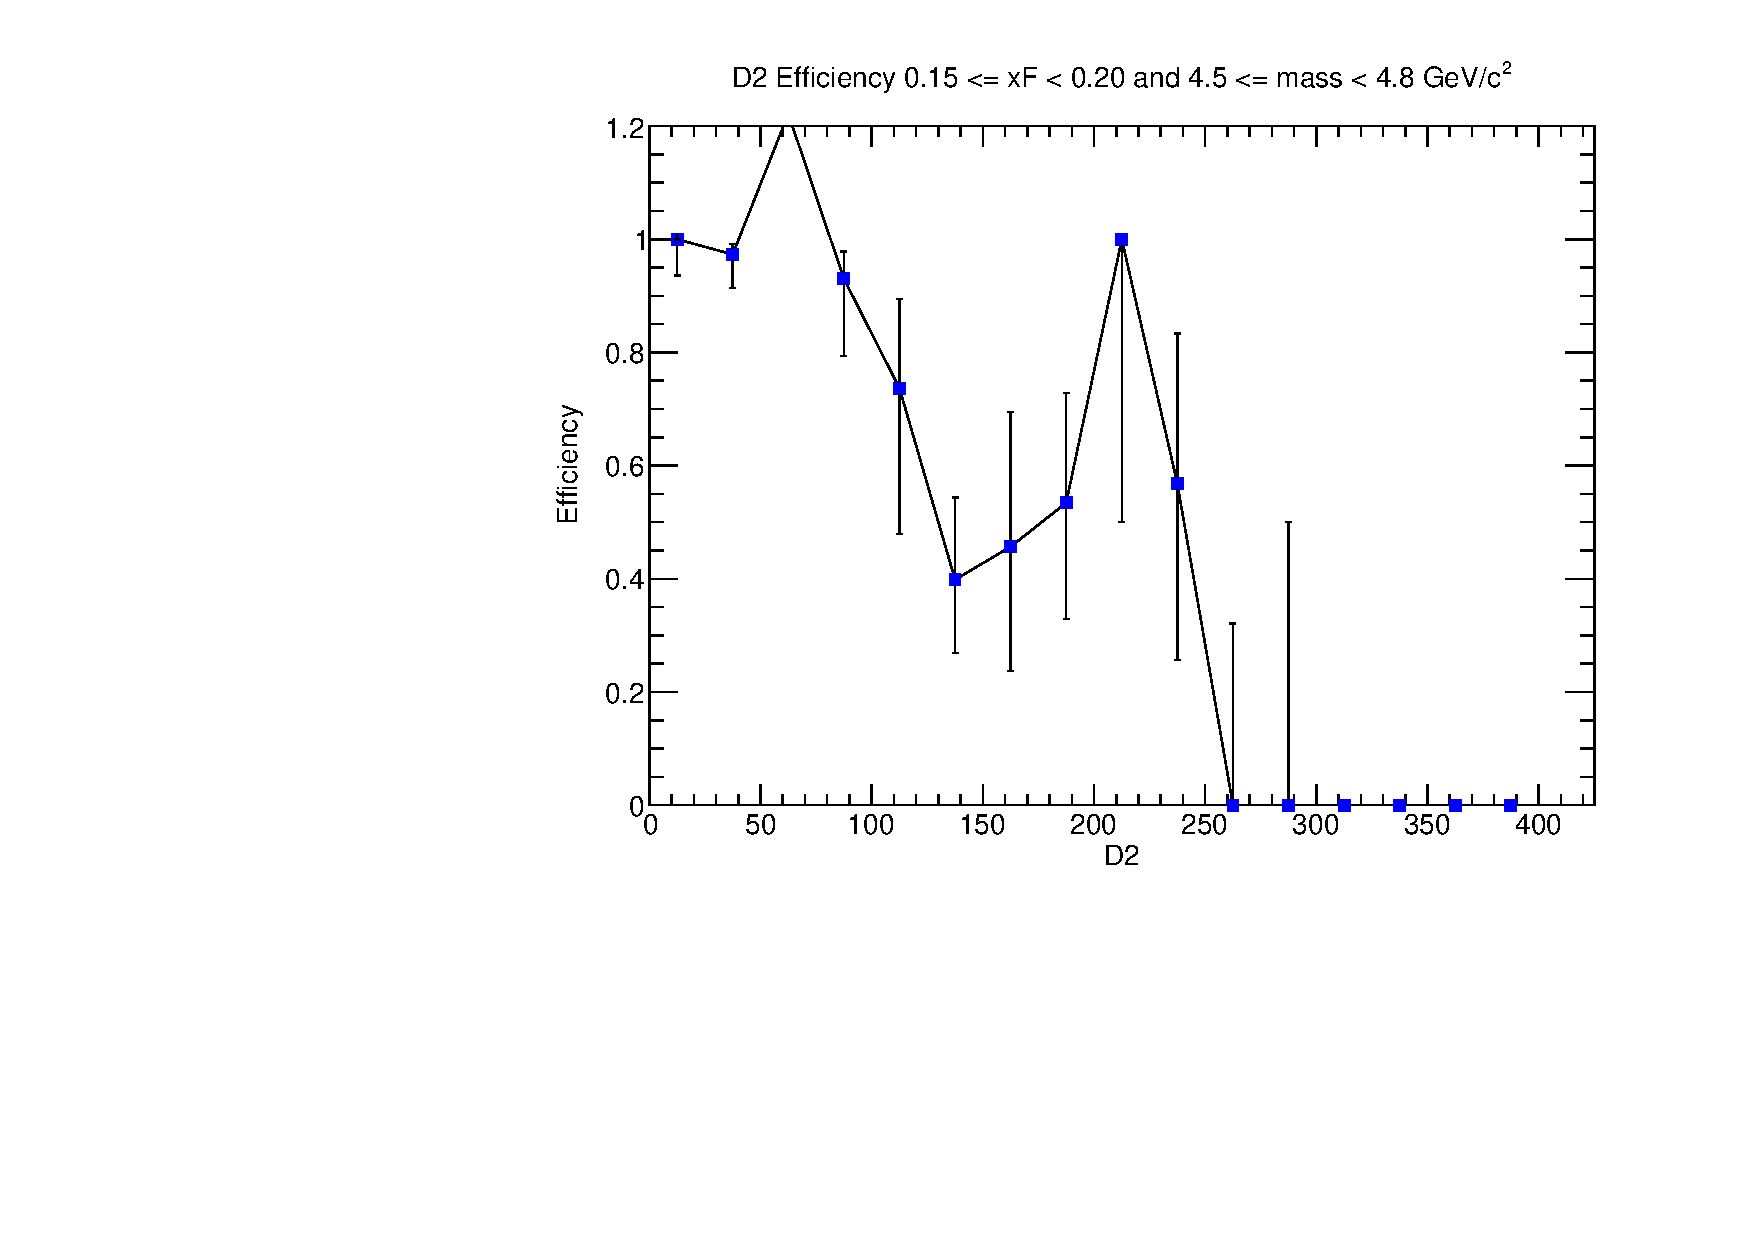
\includegraphics[width=\textwidth]{./kTrackerEfficiencyPlots/D2_Efficiency_xF3_mass1.pdf}
        \caption{$4.5 \leq m < 4.8$ GeV/$c^2$}
        \label{fig:xF3_mass1}
    \end{subfigure}
    \hfill
    \begin{subfigure}[b]{0.32\textwidth}
        \centering
        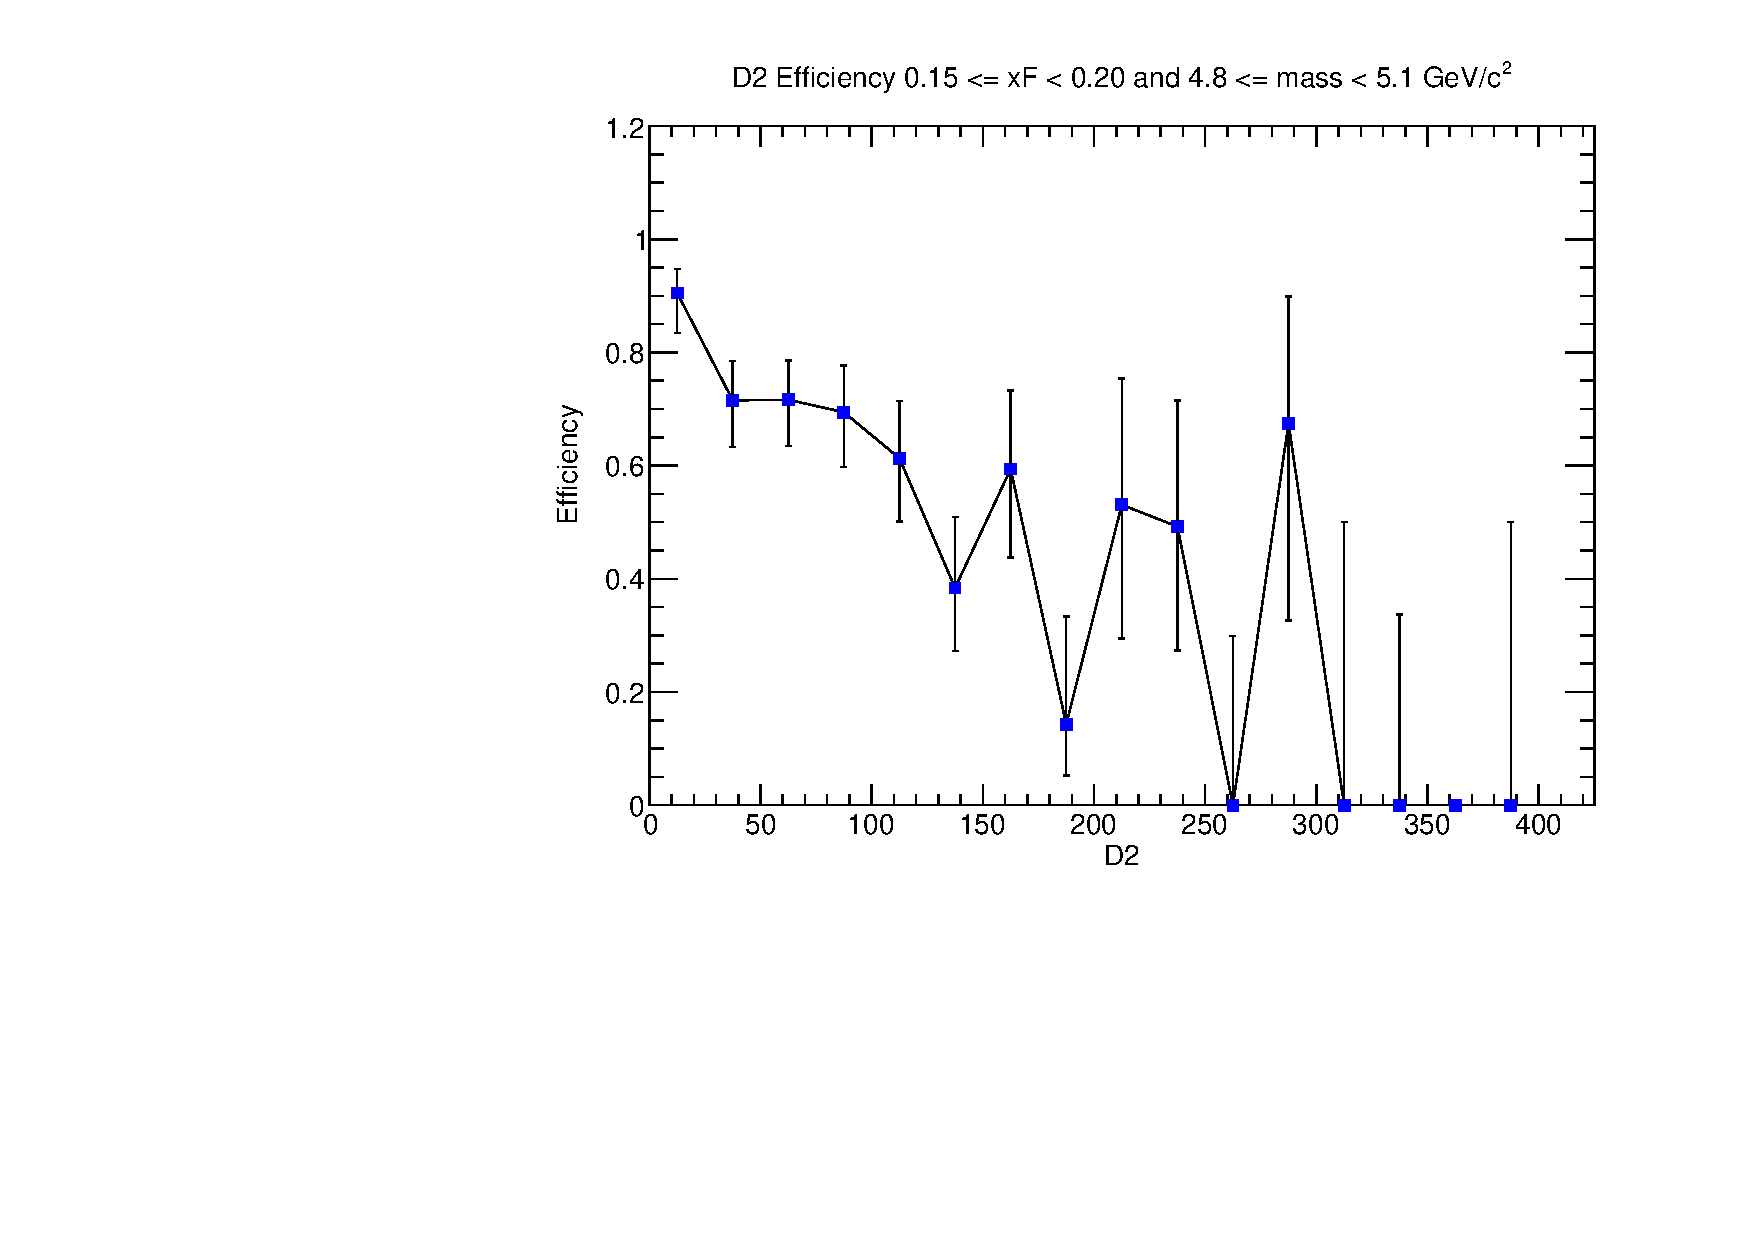
\includegraphics[width=\textwidth]{./kTrackerEfficiencyPlots/D2_Efficiency_xF3_mass2.pdf}
        \caption{$4.8 \leq m < 5.1$ GeV/$c^2$}
        \label{fig:xF3_mass2}
    \end{subfigure}
    \vspace{0.5cm}
    \begin{subfigure}[b]{0.32\textwidth}
        \centering
        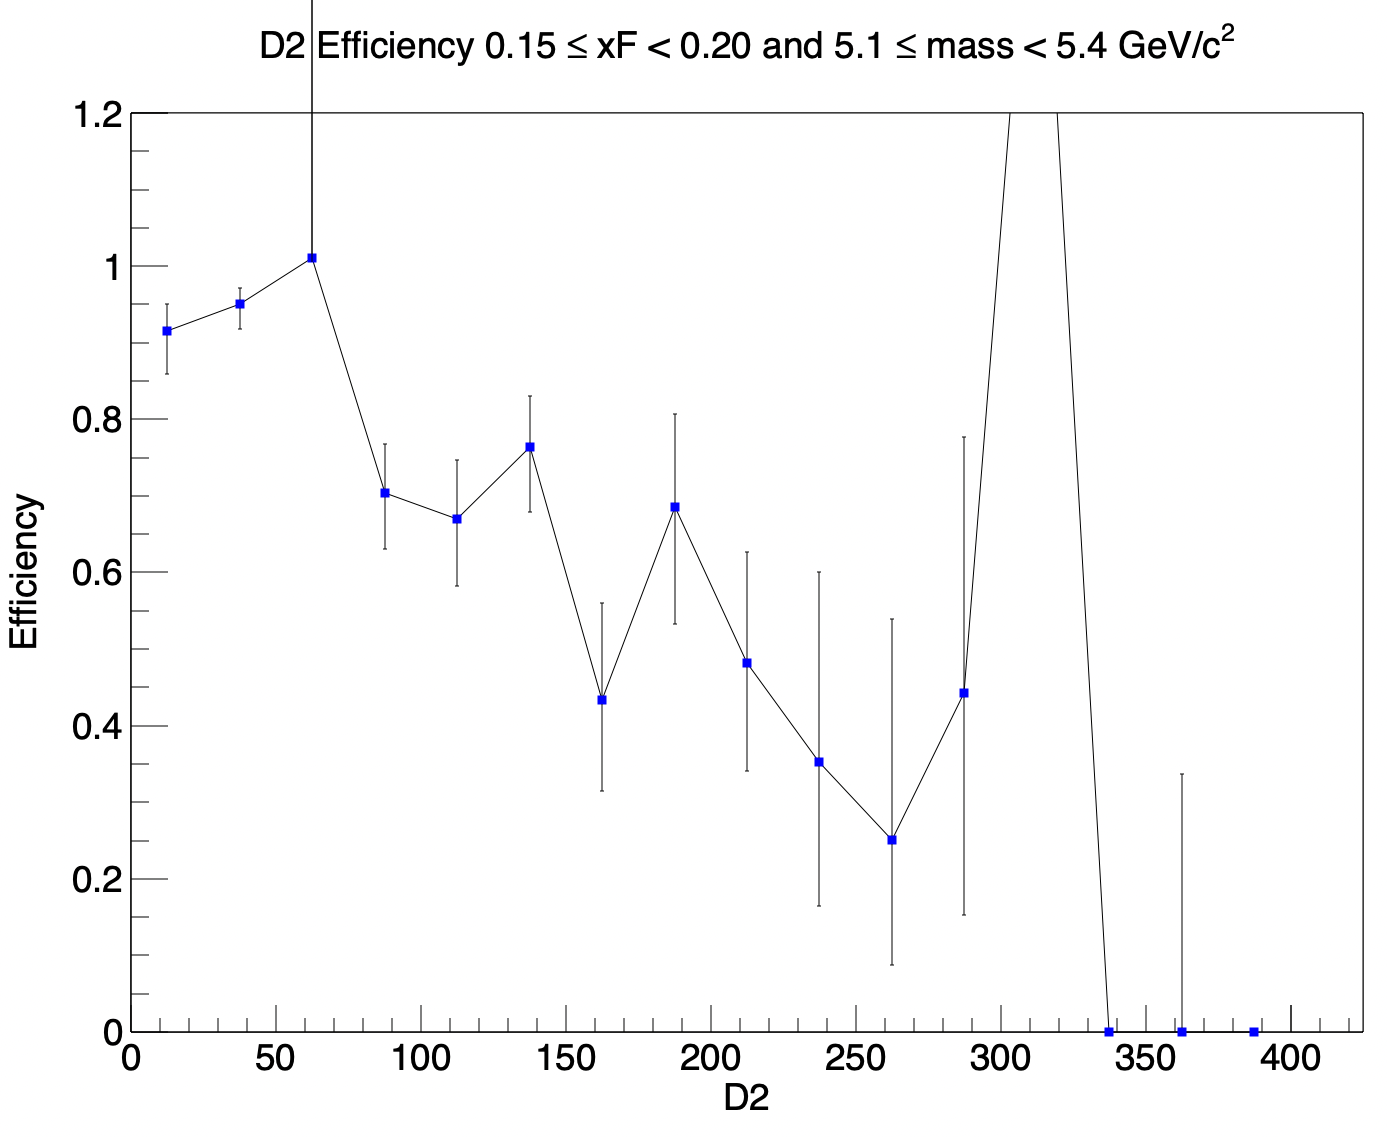
\includegraphics[width=\textwidth]{./kTrackerEfficiencyPlots/D2_Efficiency_xF3_mass3.png}
        \caption{$5.1 \leq m < 5.4$ GeV/$c^2$}
        \label{fig:xF3_mass3}
    \end{subfigure}
    \hfill
    \begin{subfigure}[b]{0.32\textwidth}
        \centering
        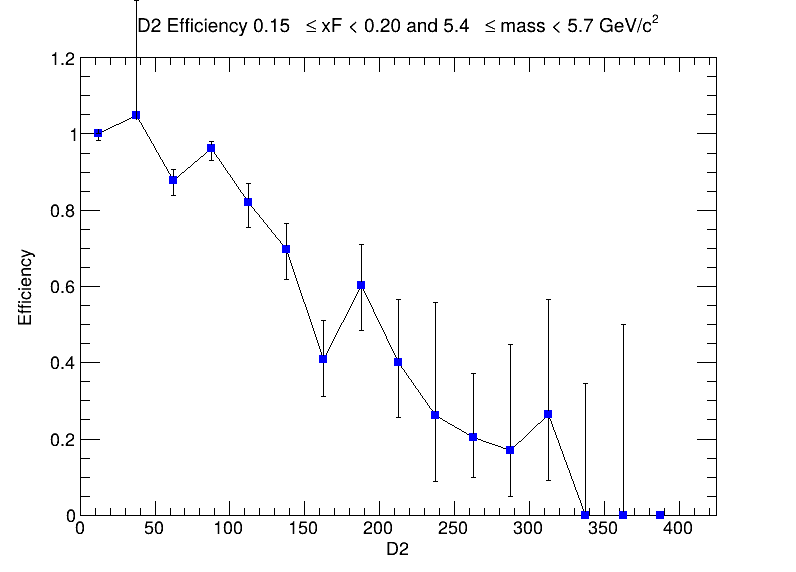
\includegraphics[width=\textwidth]{./kTrackerEfficiencyPlots/D2_Efficiency_xF3_mass4.png}
        \caption{$5.4 \leq m < 5.7$ GeV/$c^2$}
        \label{fig:xF3_mass4}
    \end{subfigure}
    \hfill
    \begin{subfigure}[b]{0.32\textwidth}
        \centering
        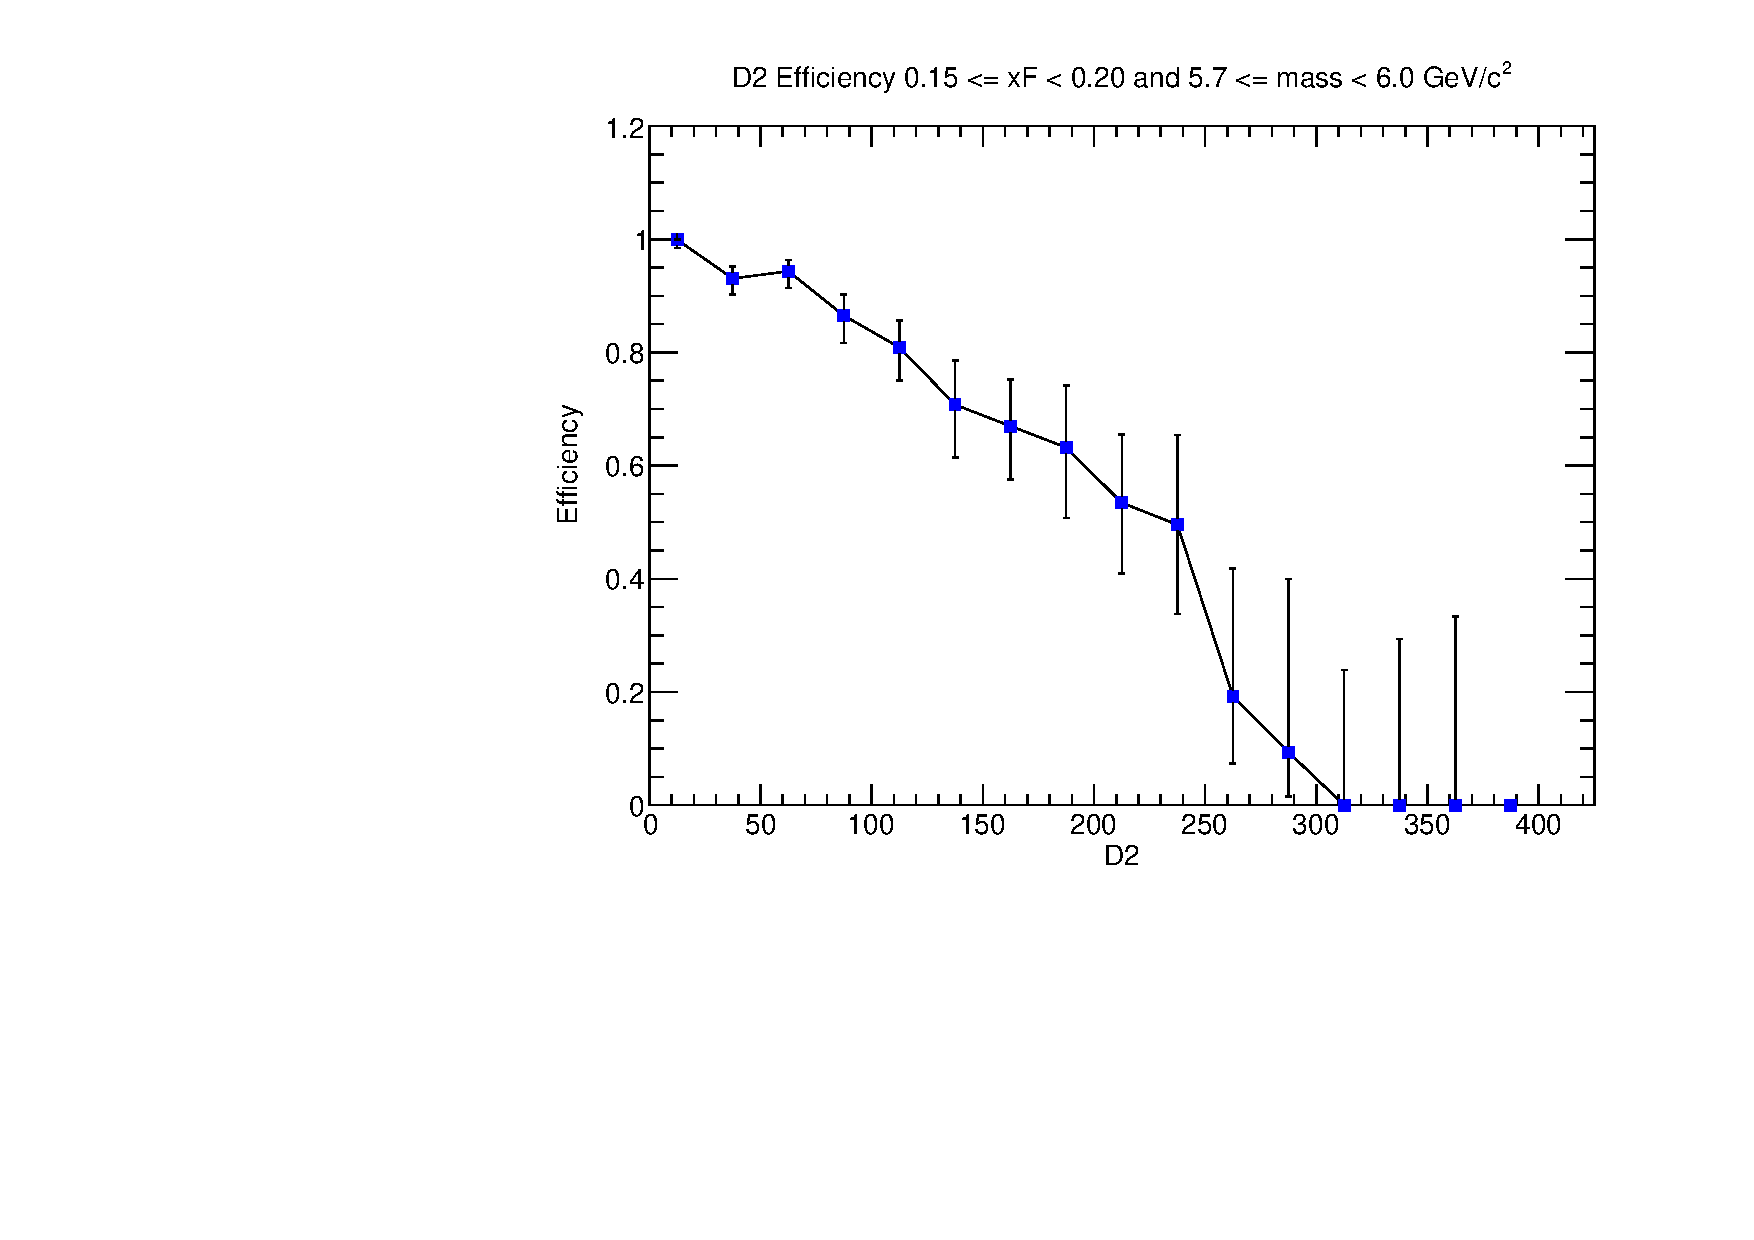
\includegraphics[width=\textwidth]{./kTrackerEfficiencyPlots/D2_Efficiency_xF3_mass5.pdf}
        \caption{$5.7 \leq m < 6.0$ GeV/$c^2$}
        \label{fig:xF3_mass5}
    \end{subfigure}
    \vspace{0.5cm}
    \begin{subfigure}[b]{0.32\textwidth}
        \centering
        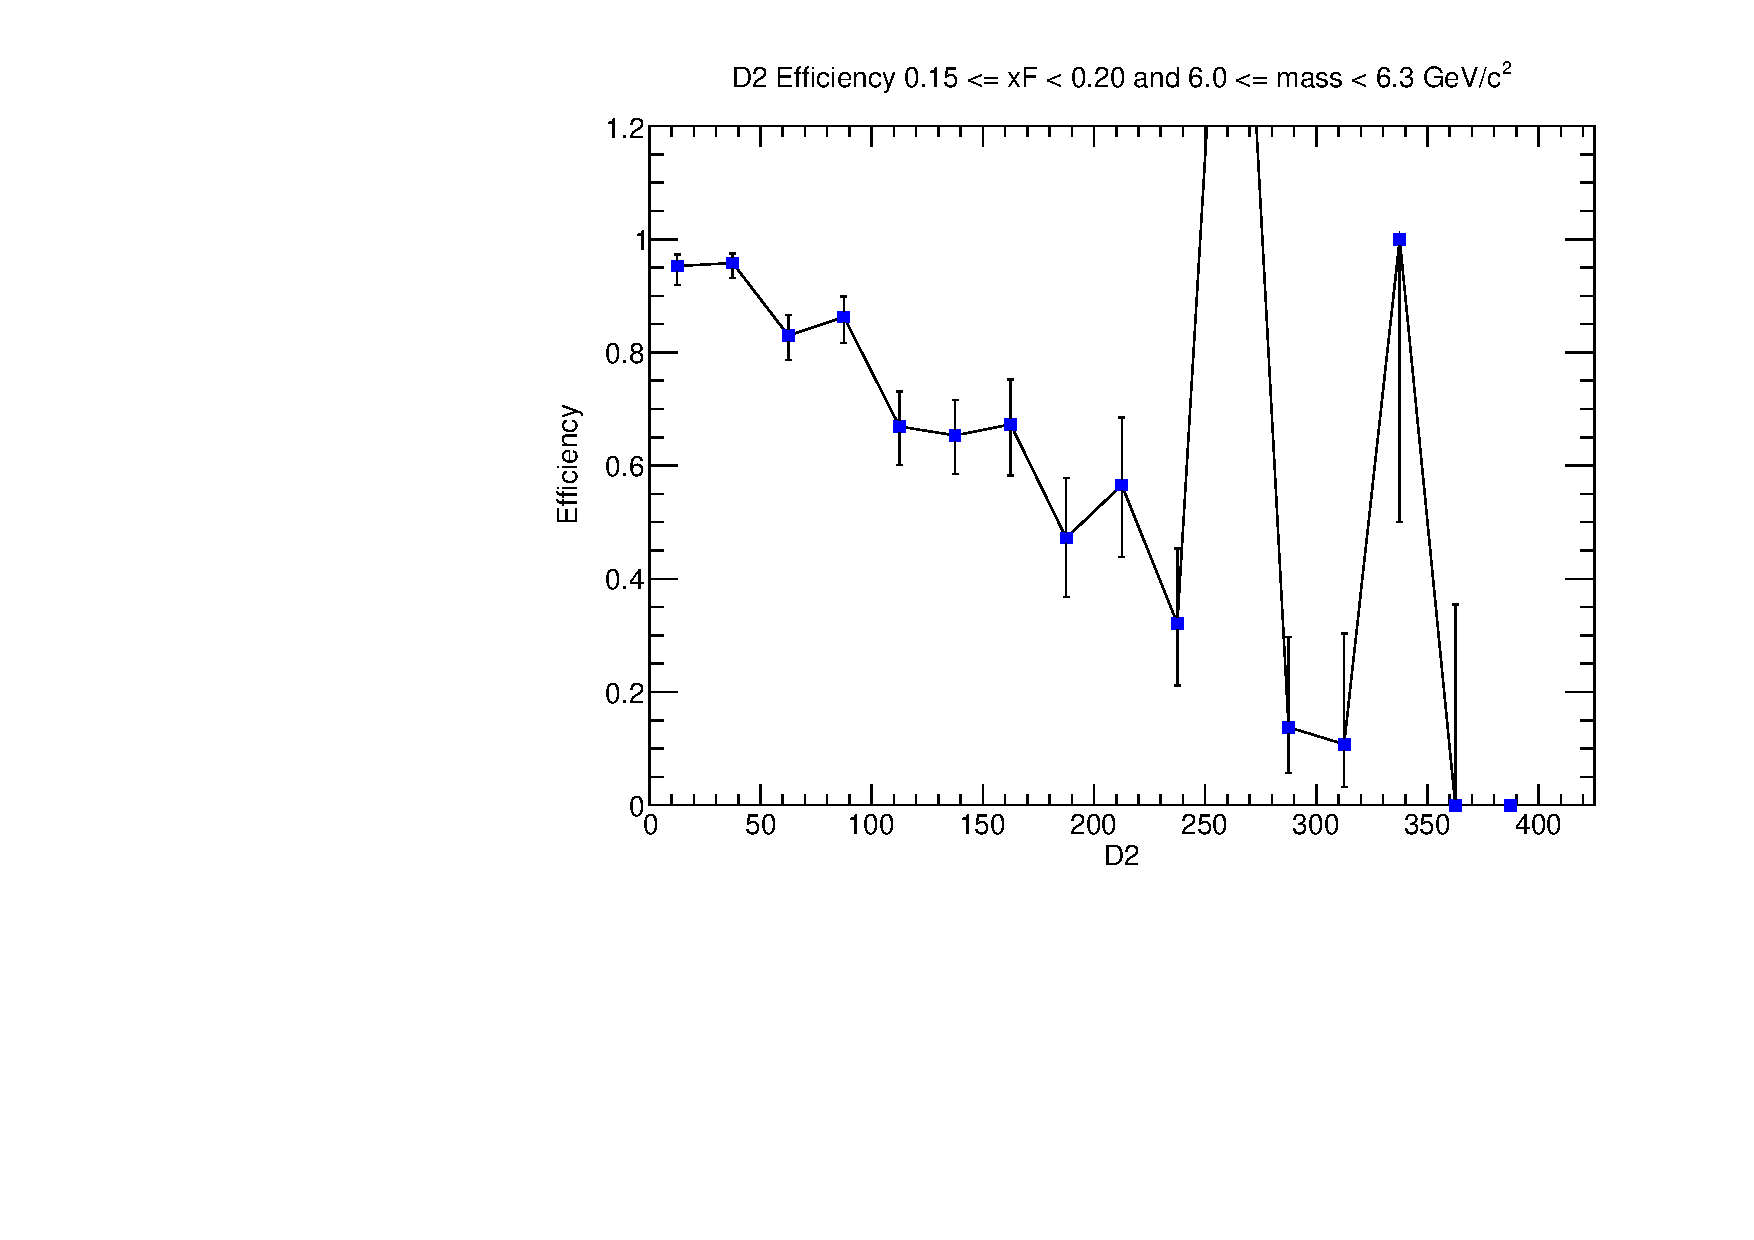
\includegraphics[width=\textwidth]{./kTrackerEfficiencyPlots/D2_Efficiency_xF3_mass6.pdf}
        \caption{$6.0 \leq m < 6.3$ GeV/$c^2$}
        \label{fig:xF3_mass6}
    \end{subfigure}
    \hfill
    \begin{subfigure}[b]{0.32\textwidth}
        \centering
        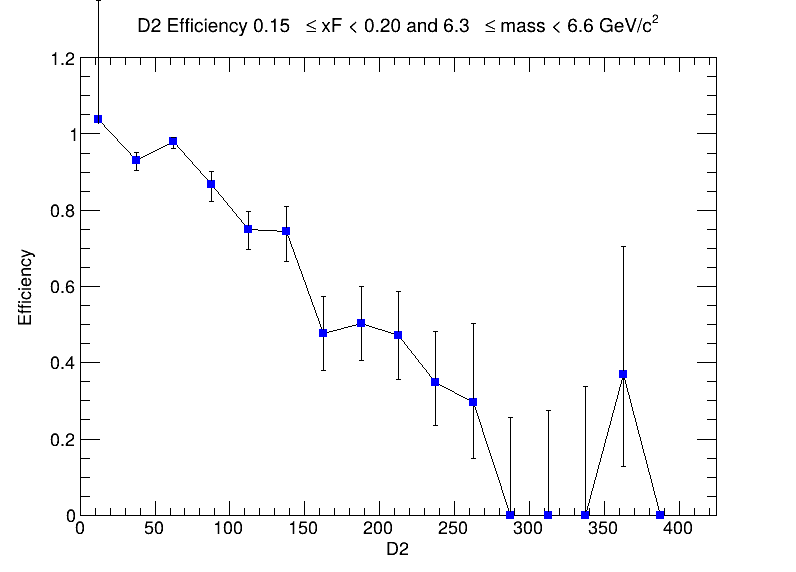
\includegraphics[width=\textwidth]{./kTrackerEfficiencyPlots/D2_Efficiency_xF3_mass7.png}
        \caption{$6.3 \leq m < 6.6$ GeV/$c^2$}
        \label{fig:xF3_mass7}
    \end{subfigure}
    \hfill
    \begin{subfigure}[b]{0.32\textwidth}
        \centering
        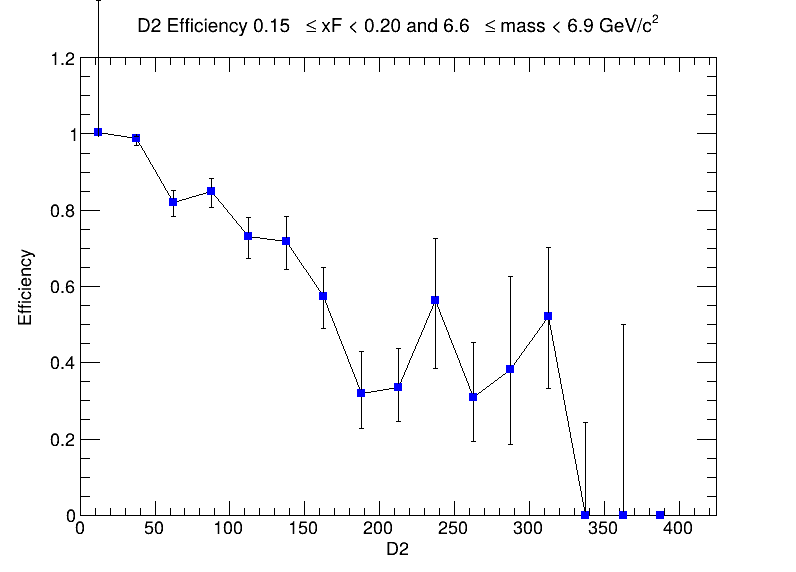
\includegraphics[width=\textwidth]{./kTrackerEfficiencyPlots/D2_Efficiency_xF3_mass8.png}
        \caption{$6.6 \leq m < 6.9$ GeV/$c^2$}
        \label{fig:xF3_mass8}
    \end{subfigure}
    \vspace{0.5cm}
    \begin{subfigure}[b]{0.32\textwidth}
        \centering
        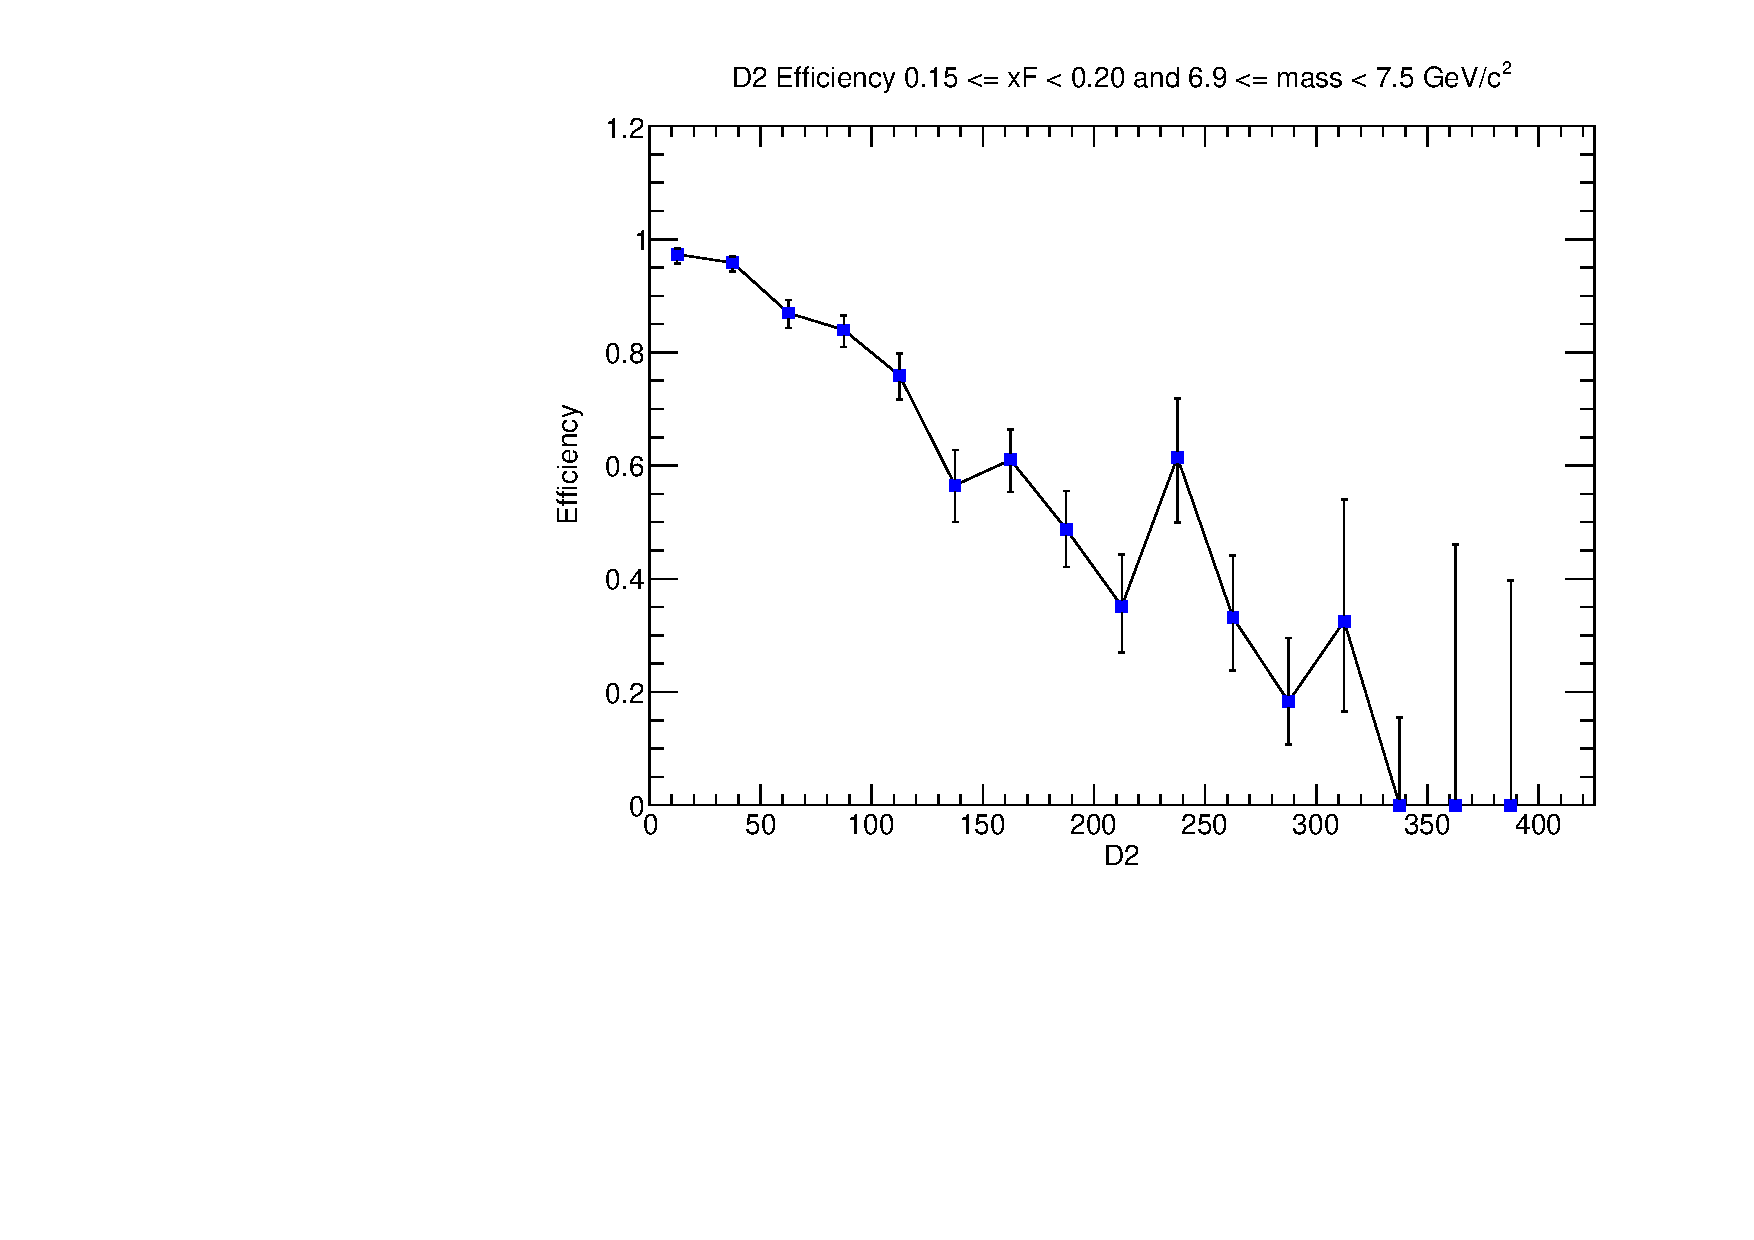
\includegraphics[width=\textwidth]{./kTrackerEfficiencyPlots/D2_Efficiency_xF3_mass9.pdf}
        \caption{$6.9 \leq m < 7.5$ GeV/$c^2$}
        \label{fig:xF3_mass9}
    \end{subfigure}
    \hfill
    \begin{subfigure}[b]{0.32\textwidth}
        \centering
        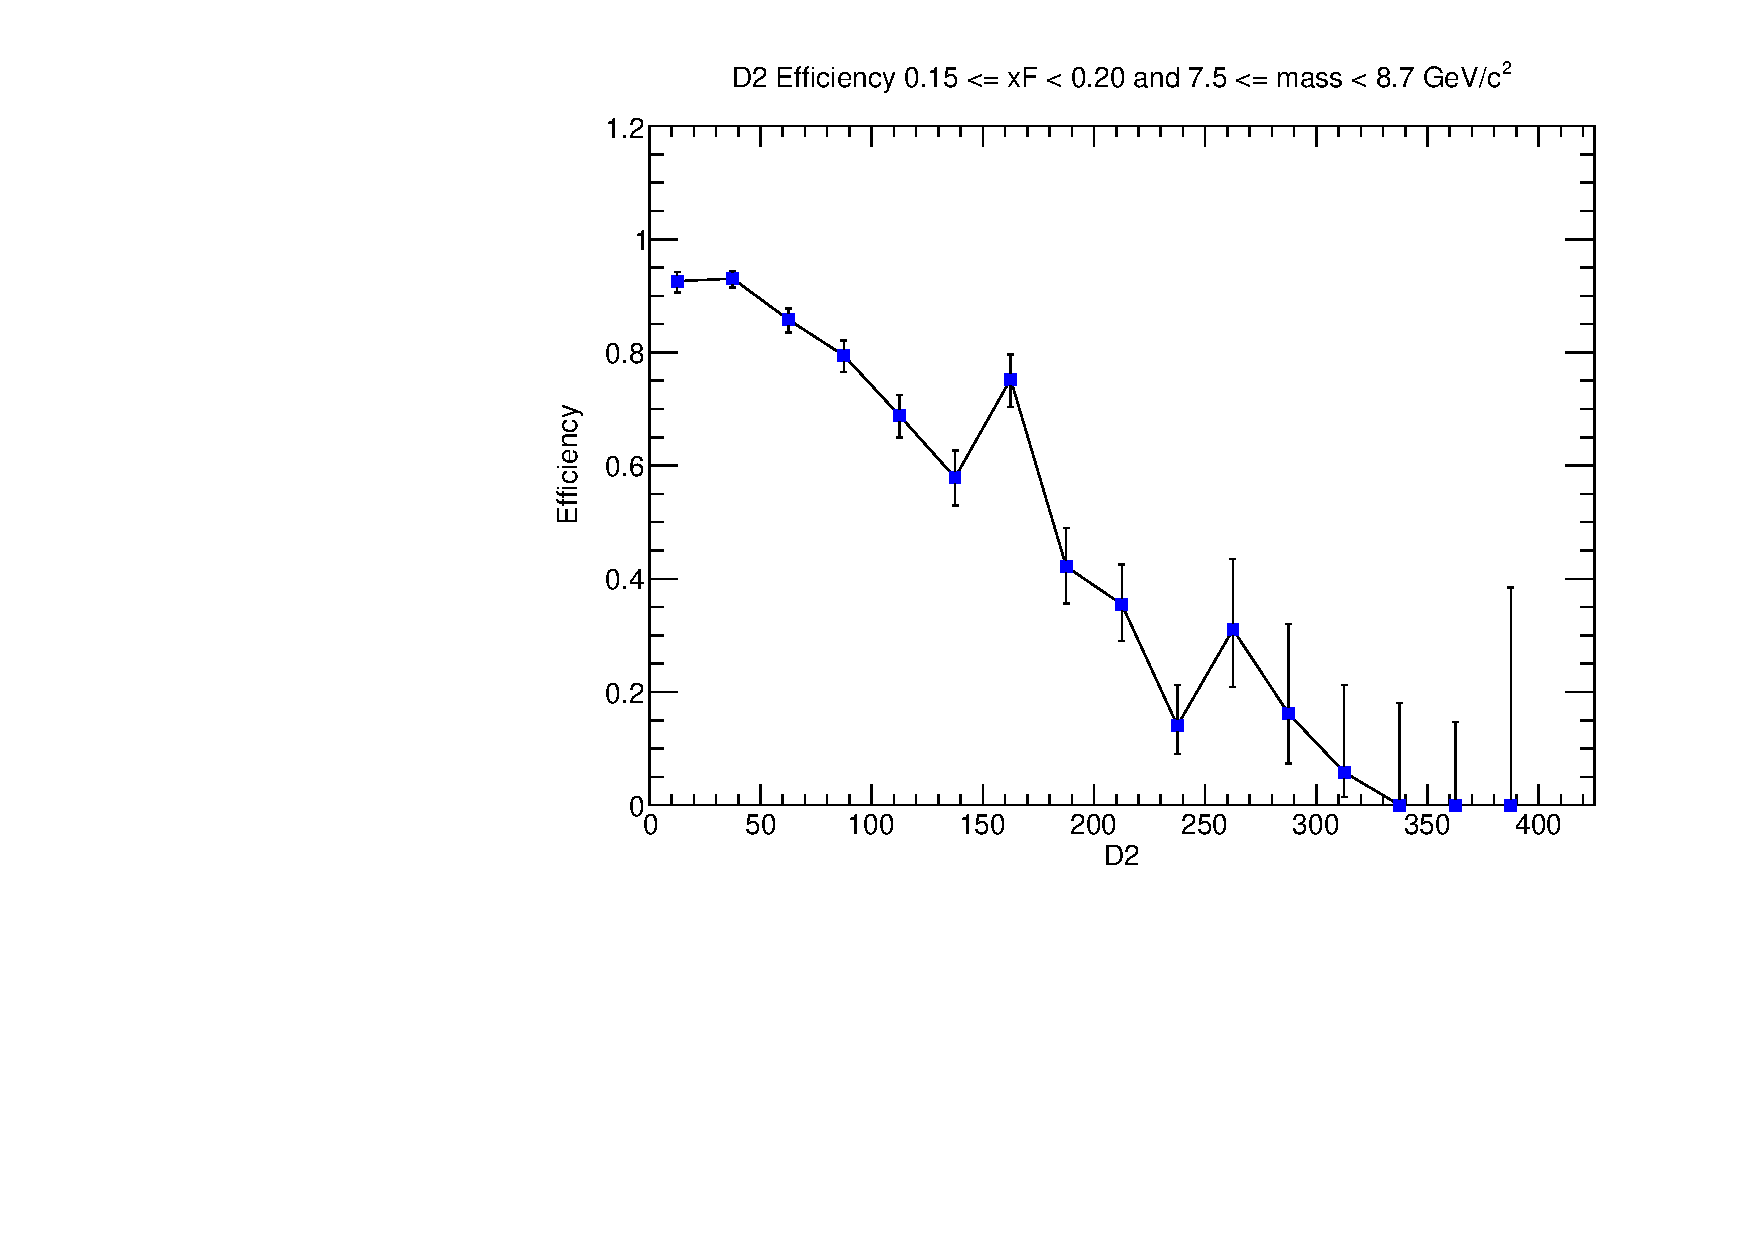
\includegraphics[width=\textwidth]{./kTrackerEfficiencyPlots/D2_Efficiency_xF3_mass10.pdf}
        \caption{$7.5 \leq m < 8.7$ GeV/$c^2$}
        \label{fig:xF3_mass10}
    \end{subfigure}
    \hfill
    \caption{Efficiency plots for the $x_F$ bin $0.15 \leq x_F < 0.20$.}
    \label{fig:xF3}
\end{figure}

\clearpage

\begin{figure}[p]
    \centering
    \begin{subfigure}[b]{0.32\textwidth}
        \centering
        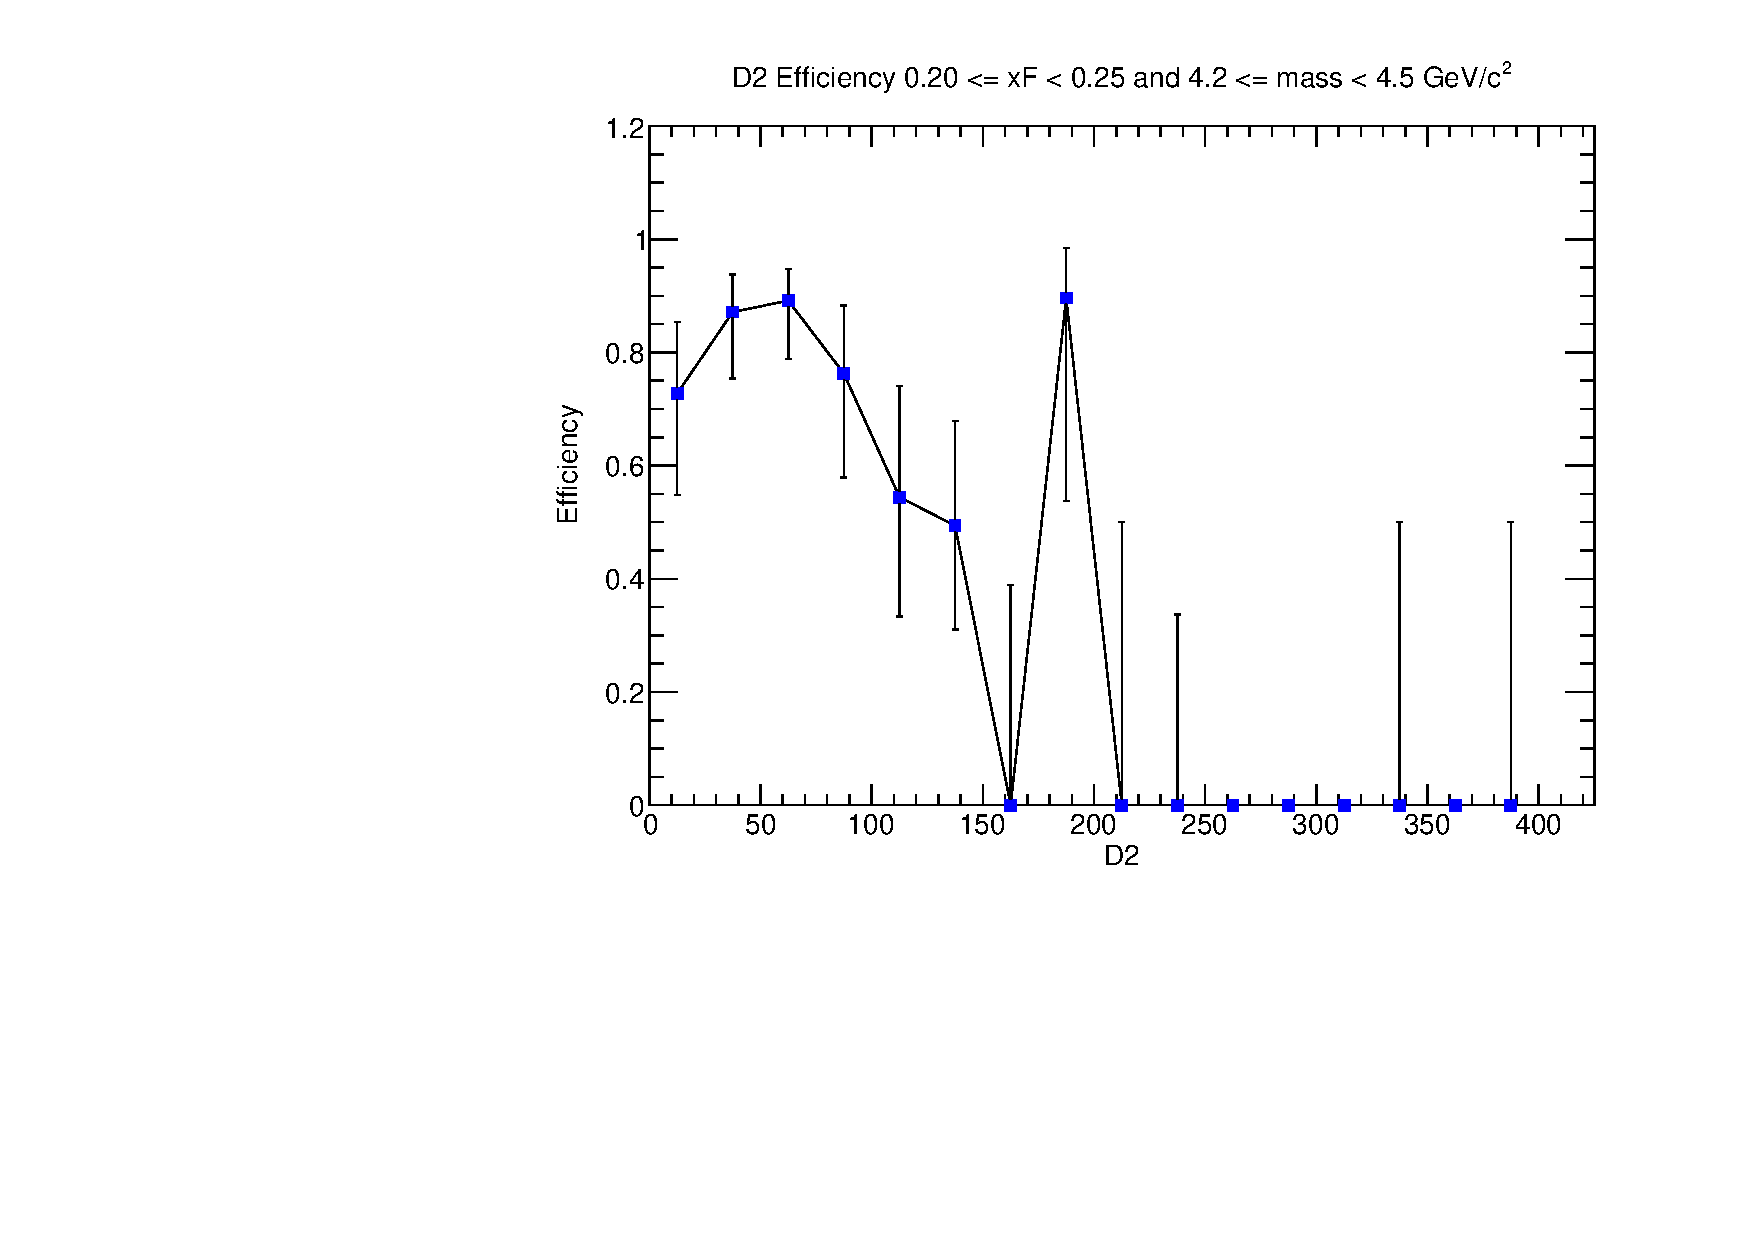
\includegraphics[width=\textwidth]{./kTrackerEfficiencyPlots/D2_Efficiency_xF4_mass0.pdf}
        \caption{$4.2 \leq m < 4.5$ GeV/$c^2$}
        \label{fig:xF4_mass0}
    \end{subfigure}
    \hfill
    \begin{subfigure}[b]{0.32\textwidth}
        \centering
        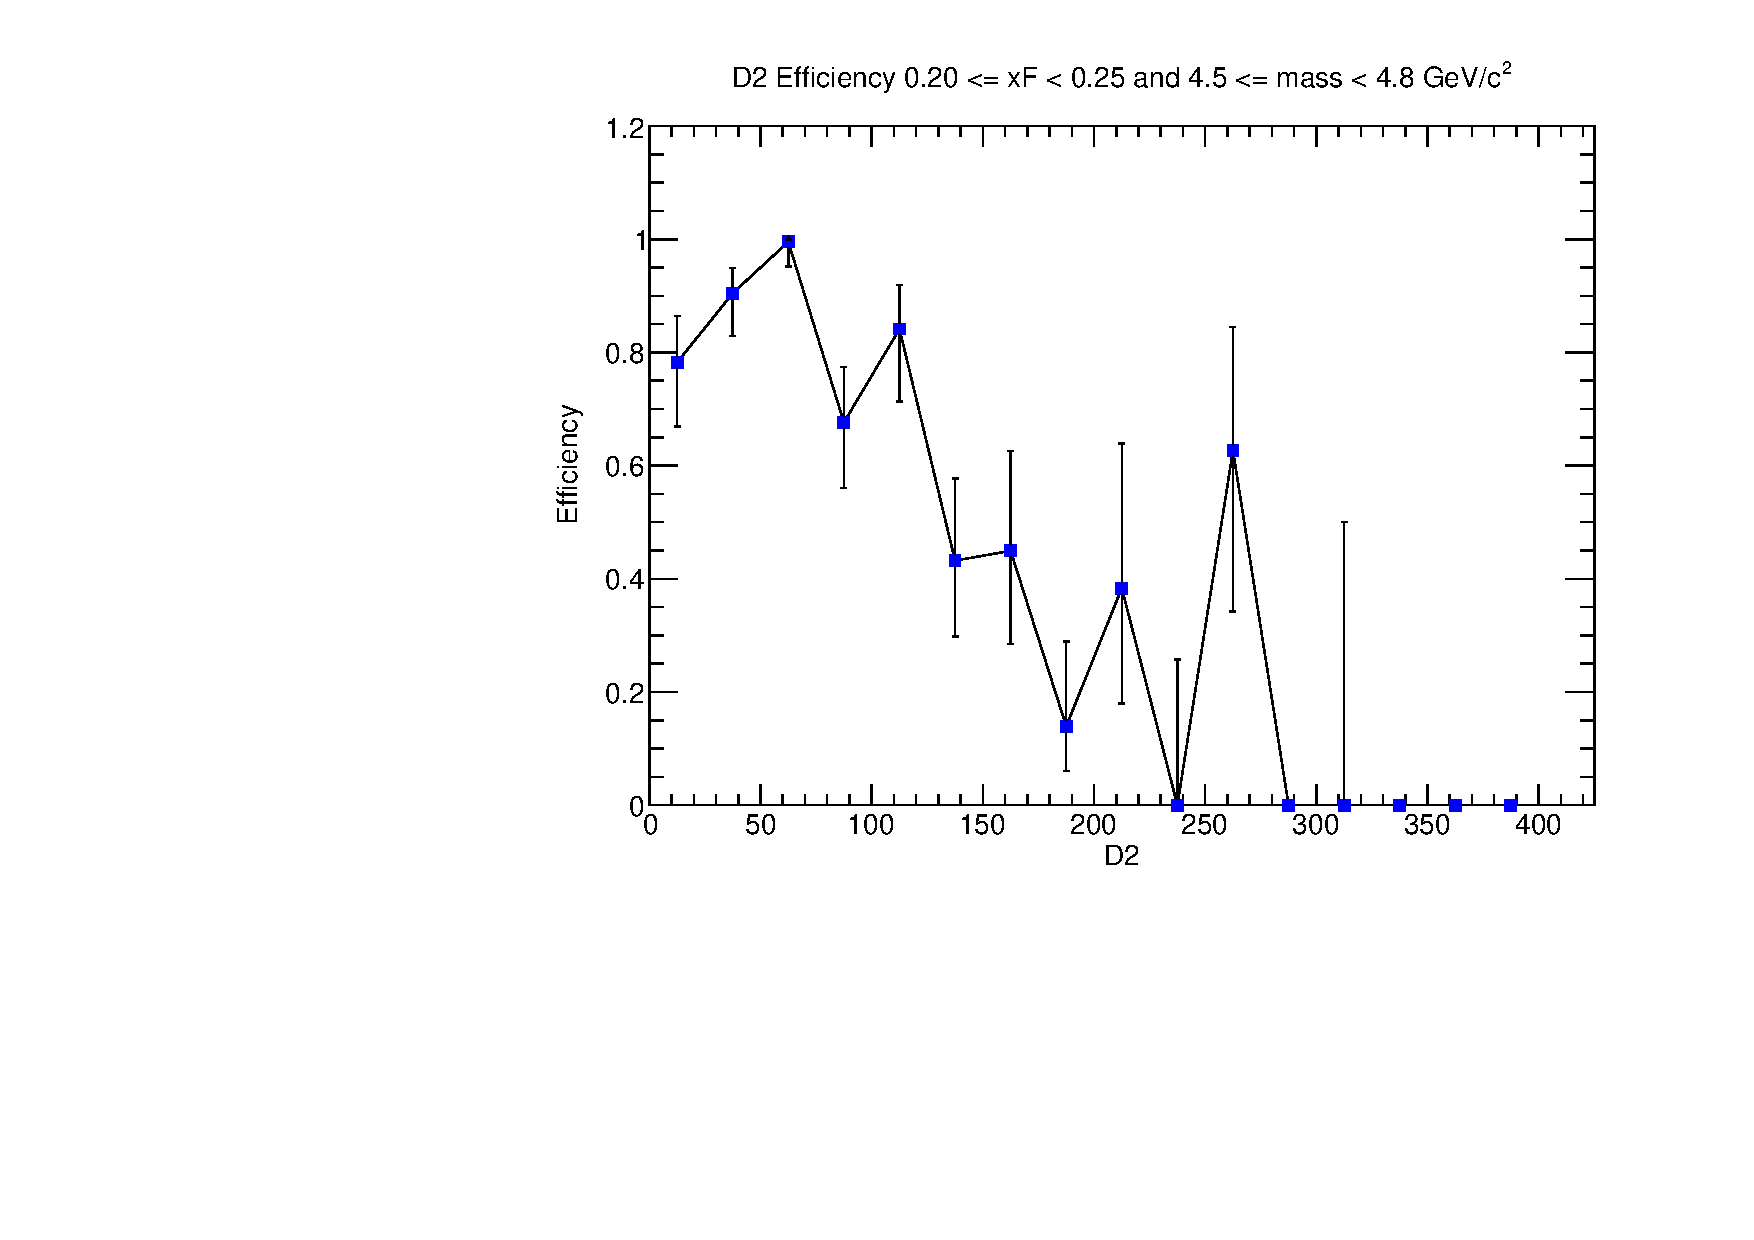
\includegraphics[width=\textwidth]{./kTrackerEfficiencyPlots/D2_Efficiency_xF4_mass1.pdf}
        \caption{$4.5 \leq m < 4.8$ GeV/$c^2$}
        \label{fig:xF4_mass1}
    \end{subfigure}
    \hfill
    \begin{subfigure}[b]{0.32\textwidth}
        \centering
        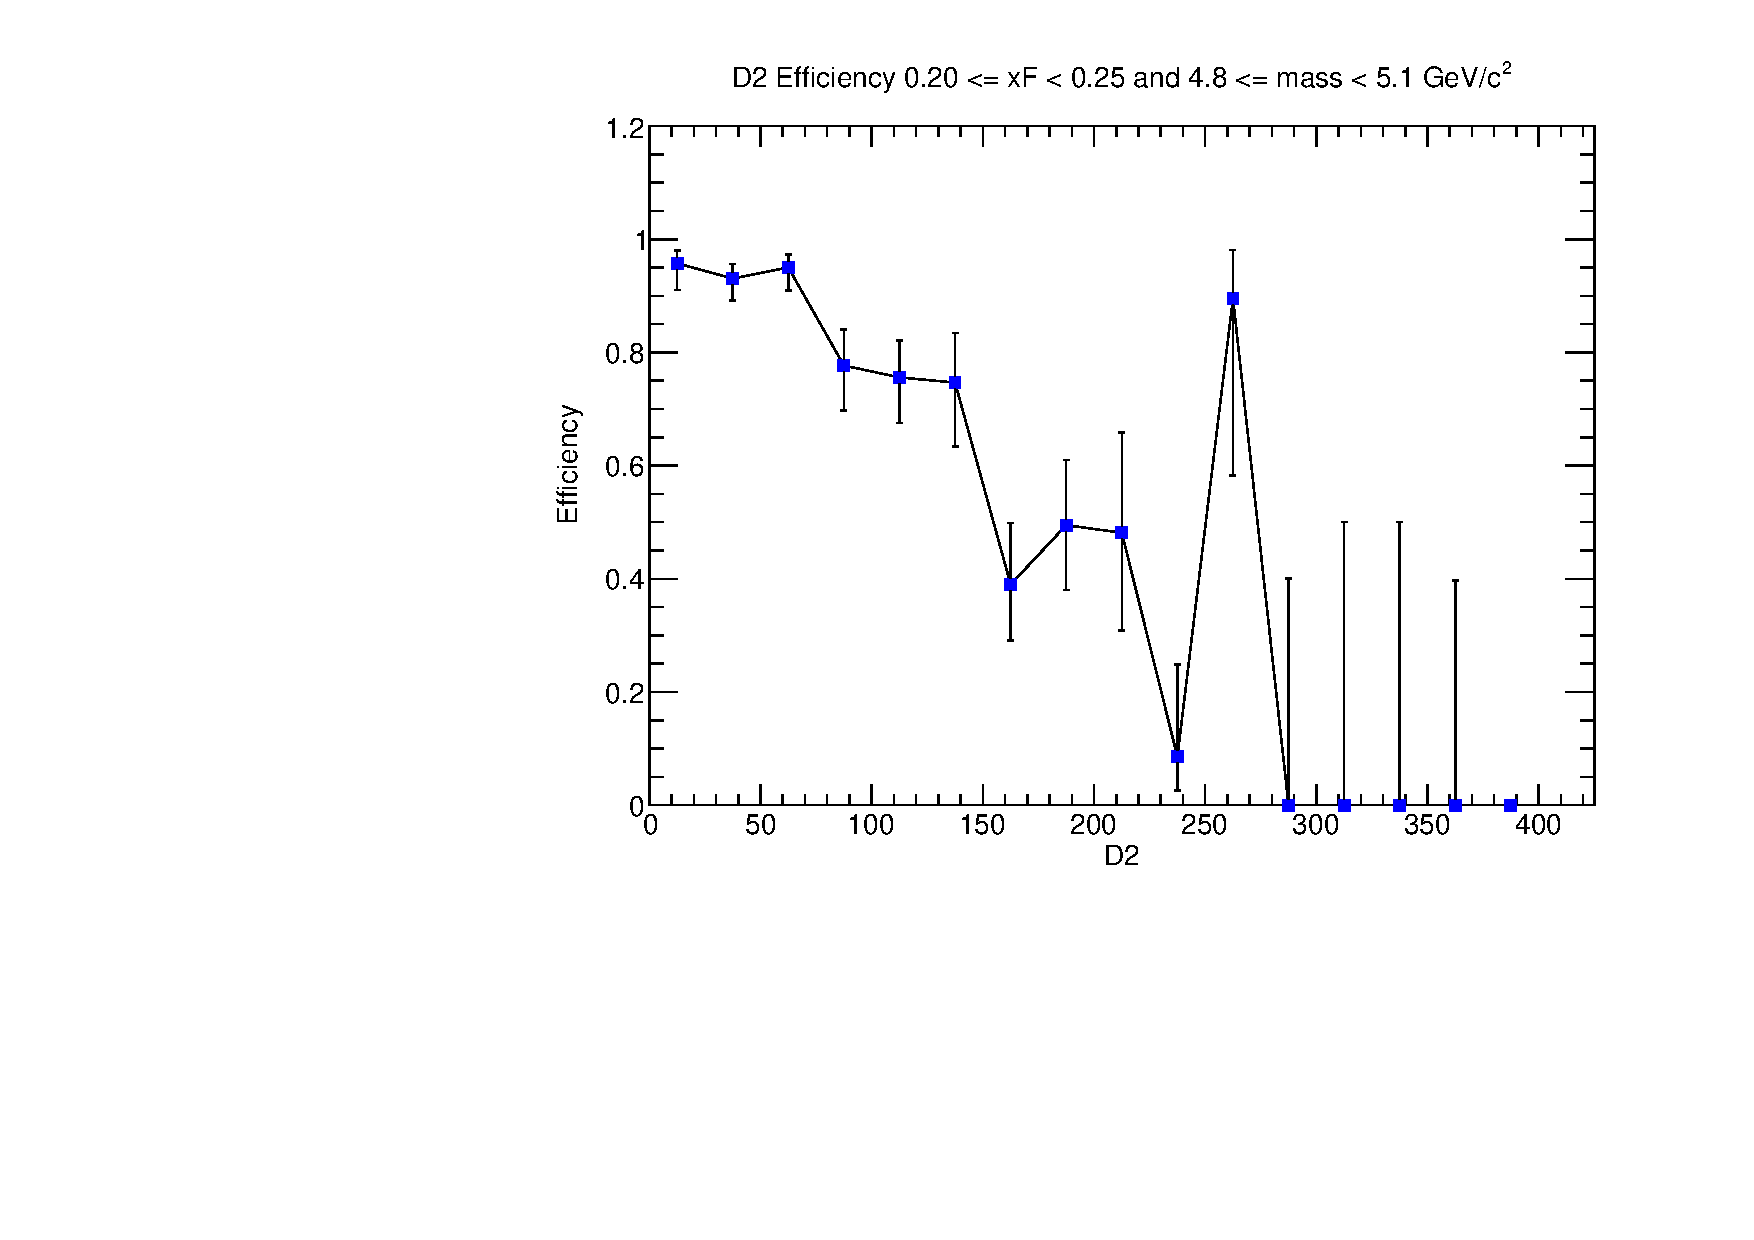
\includegraphics[width=\textwidth]{./kTrackerEfficiencyPlots/D2_Efficiency_xF4_mass2.pdf}
        \caption{$4.8 \leq m < 5.1$ GeV/$c^2$}
        \label{fig:xF4_mass2}
    \end{subfigure}
    \vspace{0.5cm}
    \begin{subfigure}[b]{0.32\textwidth}
        \centering
        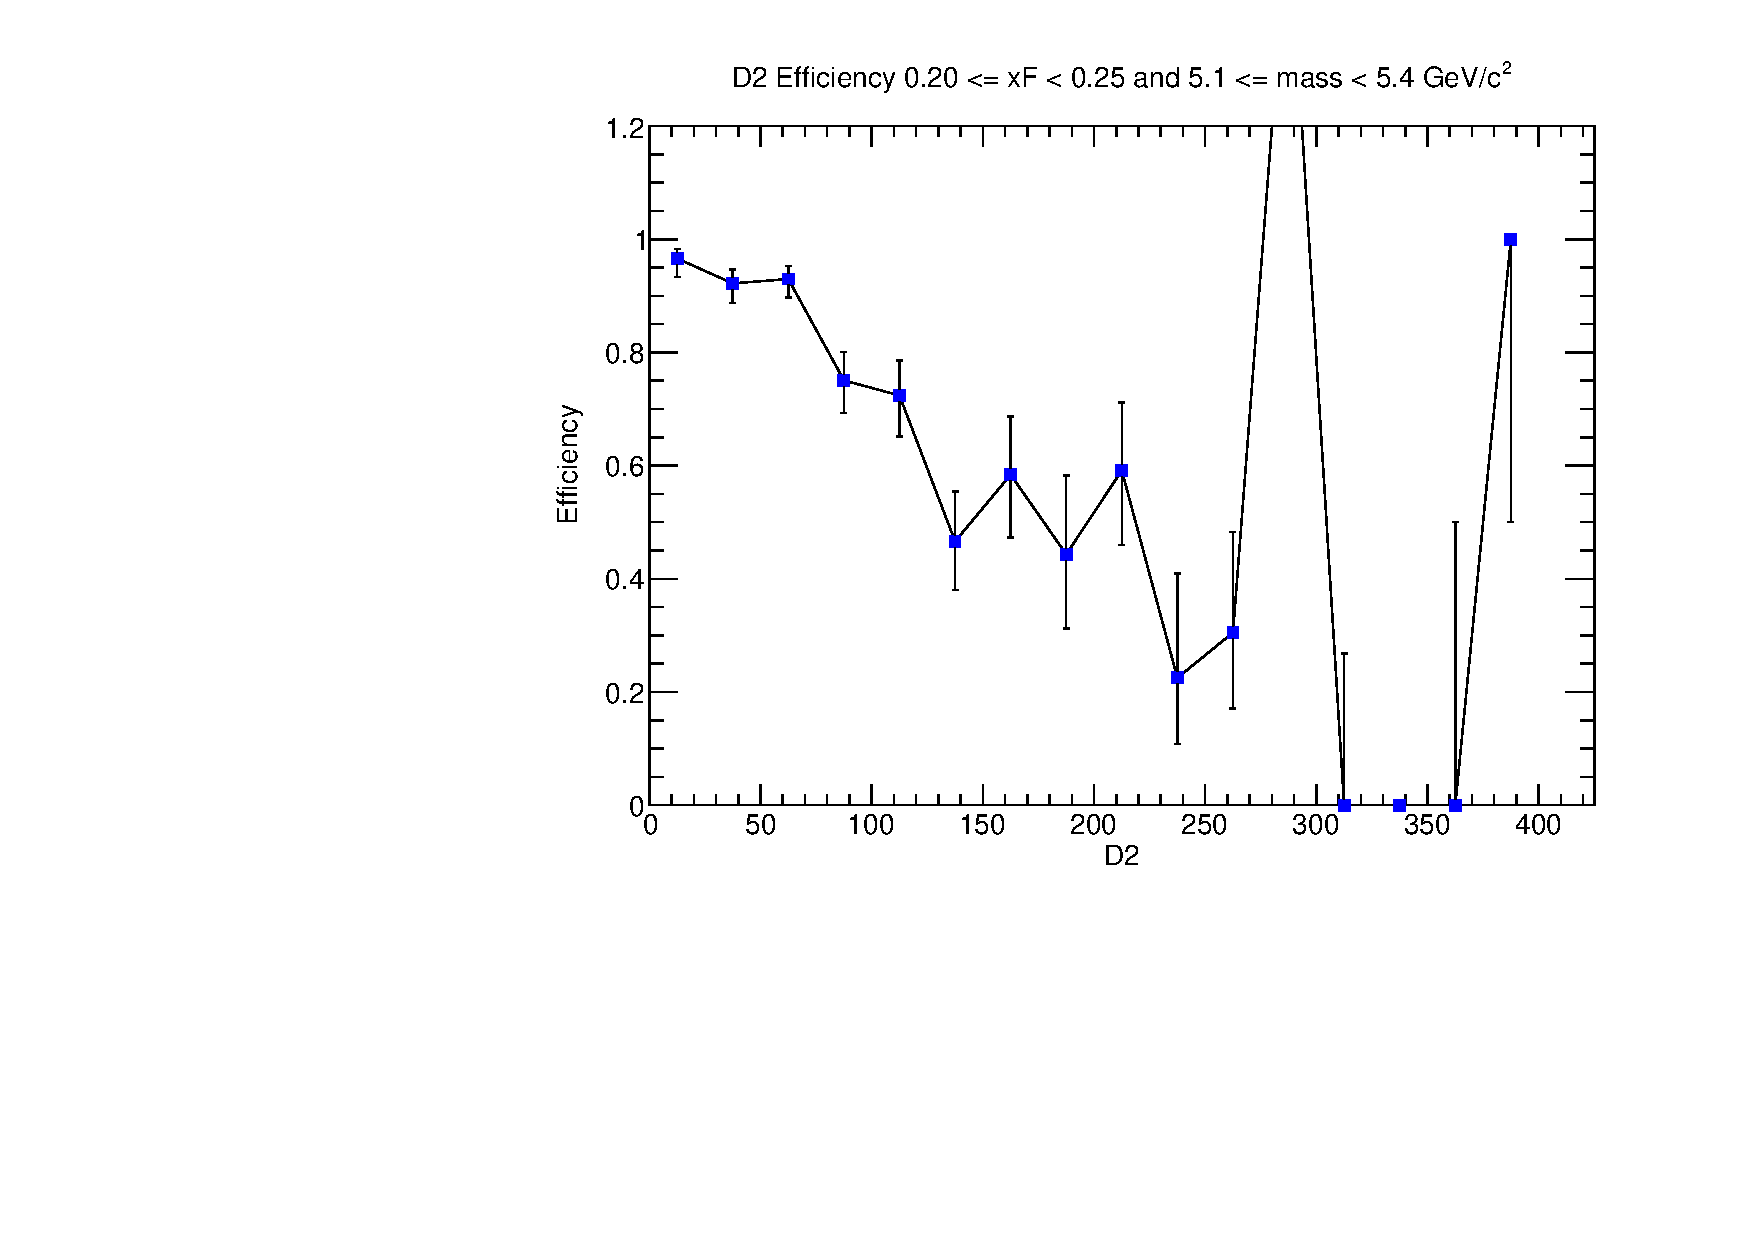
\includegraphics[width=\textwidth]{./kTrackerEfficiencyPlots/D2_Efficiency_xF4_mass3.pdf}
        \caption{$5.1 \leq m < 5.4$ GeV/$c^2$}
        \label{fig:xF4_mass3}
    \end{subfigure}
    \hfill
    \begin{subfigure}[b]{0.32\textwidth}
        \centering
        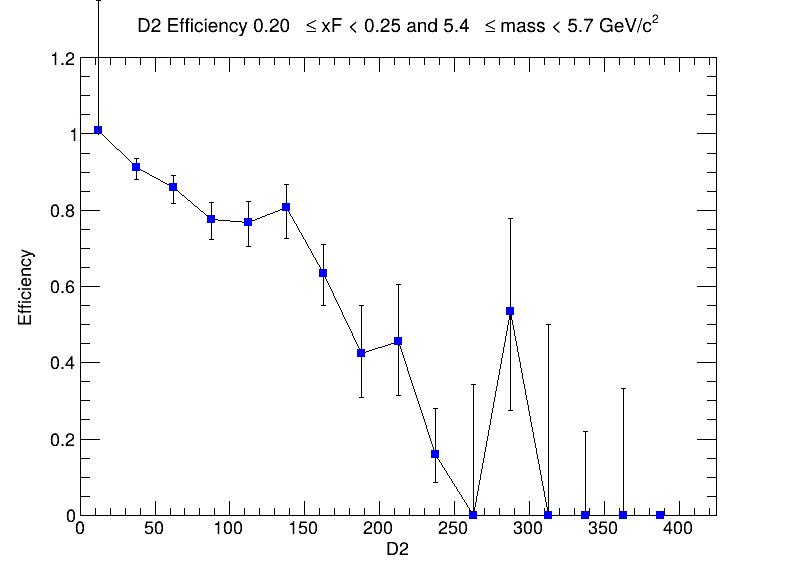
\includegraphics[width=\textwidth]{./kTrackerEfficiencyPlots/D2_Efficiency_xF4_mass4.png}
        \caption{$5.4 \leq m < 5.7$ GeV/$c^2$}
        \label{fig:xF4_mass4}
    \end{subfigure}
    \hfill
    \begin{subfigure}[b]{0.32\textwidth}
        \centering
        \includegraphics[width=\textwidth]{./kTrackerEfficiencyPlots/D2_Efficiency_xF4_mass5.pdf}
        \caption{$5.7 \leq m < 6.0$ GeV/$c^2$}
        \label{fig:xF4_mass5}
    \end{subfigure}
    \vspace{0.5cm}
    \begin{subfigure}[b]{0.32\textwidth}
        \centering
        \includegraphics[width=\textwidth]{./kTrackerEfficiencyPlots/D2_Efficiency_xF4_mass6.png}
        \caption{$6.0 \leq m < 6.3$ GeV/$c^2$}
        \label{fig:xF4_mass6}
    \end{subfigure}
    \hfill
    \begin{subfigure}[b]{0.32\textwidth}
        \centering
        \includegraphics[width=\textwidth]{./kTrackerEfficiencyPlots/D2_Efficiency_xF4_mass7.pdf}
        \caption{$6.3 \leq m < 6.6$ GeV/$c^2$}
        \label{fig:xF4_mass7}
    \end{subfigure}
    \hfill
    \begin{subfigure}[b]{0.32\textwidth}
        \centering
        \includegraphics[width=\textwidth]{./kTrackerEfficiencyPlots/D2_Efficiency_xF4_mass8.pdf}
        \caption{$6.6 \leq m < 6.9$ GeV/$c^2$}
        \label{fig:xF4_mass8}
    \end{subfigure}
    \vspace{0.5cm}
    \begin{subfigure}[b]{0.32\textwidth}
        \centering
        \includegraphics[width=\textwidth]{./kTrackerEfficiencyPlots/D2_Efficiency_xF4_mass9.png}
        \caption{$6.9 \leq m < 7.5$ GeV/$c^2$}
        \label{fig:xF4_mass9}
    \end{subfigure}
    \hfill
    \begin{subfigure}[b]{0.32\textwidth}
        \centering
        \includegraphics[width=\textwidth]{./kTrackerEfficiencyPlots/D2_Efficiency_xF4_mass10.pdf}
        \caption{$7.5 \leq m < 8.7$ GeV/$c^2$}
        \label{fig:xF4_mass10}
    \end{subfigure}
    \hfill
    \caption{Efficiency plots for the $x_F$ bin $0.20 \leq x_F < 0.25$.}
    \label{fig:xF4}
\end{figure}

\clearpage

\begin{figure}[p]
    \centering
    \begin{subfigure}[b]{0.32\textwidth}
        \centering
        \includegraphics[width=\textwidth]{./kTrackerEfficiencyPlots/D2_Efficiency_xF5_mass0.png}
        \caption{$4.2 \leq m < 4.5$ GeV/$c^2$}
        \label{fig:xF5_mass0}
    \end{subfigure}
    \hfill
    \begin{subfigure}[b]{0.32\textwidth}
        \centering
        \includegraphics[width=\textwidth]{./kTrackerEfficiencyPlots/D2_Efficiency_xF5_mass1.pdf}
        \caption{$4.5 \leq m < 4.8$ GeV/$c^2$}
        \label{fig:xF5_mass1}
    \end{subfigure}
    \hfill
    \begin{subfigure}[b]{0.32\textwidth}
        \centering
        \includegraphics[width=\textwidth]{./kTrackerEfficiencyPlots/D2_Efficiency_xF5_mass2.pdf}
        \caption{$4.8 \leq m < 5.1$ GeV/$c^2$}
        \label{fig:xF5_mass2}
    \end{subfigure}
    \vspace{0.5cm}
    \begin{subfigure}[b]{0.32\textwidth}
        \centering
        \includegraphics[width=\textwidth]{./kTrackerEfficiencyPlots/D2_Efficiency_xF5_mass3.pdf}
        \caption{$5.1 \leq m < 5.4$ GeV/$c^2$}
        \label{fig:xF5_mass3}
    \end{subfigure}
    \hfill
    \begin{subfigure}[b]{0.32\textwidth}
        \centering
        \includegraphics[width=\textwidth]{./kTrackerEfficiencyPlots/D2_Efficiency_xF5_mass4.png}
        \caption{$5.4 \leq m < 5.7$ GeV/$c^2$}
        \label{fig:xF5_mass4}
    \end{subfigure}
    \hfill
    \begin{subfigure}[b]{0.32\textwidth}
        \centering
        \includegraphics[width=\textwidth]{./kTrackerEfficiencyPlots/D2_Efficiency_xF5_mass5.png}
        \caption{$5.7 \leq m < 6.0$ GeV/$c^2$}
        \label{fig:xF5_mass5}
    \end{subfigure}
    \vspace{0.5cm}
    \begin{subfigure}[b]{0.32\textwidth}
        \centering
        \includegraphics[width=\textwidth]{./kTrackerEfficiencyPlots/D2_Efficiency_xF5_mass6.pdf}
        \caption{$6.0 \leq m < 6.3$ GeV/$c^2$}
        \label{fig:xF5_mass6}
    \end{subfigure}
    \hfill
    \begin{subfigure}[b]{0.32\textwidth}
        \centering
        \includegraphics[width=\textwidth]{./kTrackerEfficiencyPlots/D2_Efficiency_xF5_mass7.png}
        \caption{$6.3 \leq m < 6.6$ GeV/$c^2$}
        \label{fig:xF5_mass7}
    \end{subfigure}
    \hfill
    \begin{subfigure}[b]{0.32\textwidth}
        \centering
        \includegraphics[width=\textwidth]{./kTrackerEfficiencyPlots/D2_Efficiency_xF5_mass8.pdf}
        \caption{$6.6 \leq m < 6.9$ GeV/$c^2$}
        \label{fig:xF5_mass8}
    \end{subfigure}
    \vspace{0.5cm}
    \begin{subfigure}[b]{0.32\textwidth}
        \centering
        \includegraphics[width=\textwidth]{./kTrackerEfficiencyPlots/D2_Efficiency_xF5_mass9.pdf}
        \caption{$6.9 \leq m < 7.5$ GeV/$c^2$}
        \label{fig:xF5_mass9}
    \end{subfigure}
    \hfill
    \begin{subfigure}[b]{0.32\textwidth}
        \centering
        \includegraphics[width=\textwidth]{./kTrackerEfficiencyPlots/D2_Efficiency_xF5_mass10.pdf}
        \caption{$7.5 \leq m < 8.7$ GeV/$c^2$}
        \label{fig:xF5_mass10}
    \end{subfigure}
    \hfill
    \caption{Efficiency plots for the $x_F$ bin $0.25 \leq x_F < 0.30$.}
    \label{fig:xF5}
\end{figure}

\clearpage

\begin{figure}[p]
    \centering
    \begin{subfigure}[b]{0.32\textwidth}
        \centering
        \includegraphics[width=\textwidth]{./kTrackerEfficiencyPlots/D2_Efficiency_xF6_mass0.pdf}
        \caption{$4.2 \leq m < 4.5$ GeV/$c^2$}
        \label{fig:xF6_mass0}
    \end{subfigure}
    \hfill
    \begin{subfigure}[b]{0.32\textwidth}
        \centering
        \includegraphics[width=\textwidth]{./kTrackerEfficiencyPlots/D2_Efficiency_xF6_mass1.pdf}
        \caption{$4.5 \leq m < 4.8$ GeV/$c^2$}
        \label{fig:xF6_mass1}
    \end{subfigure}
    \hfill
    \begin{subfigure}[b]{0.32\textwidth}
        \centering
        \includegraphics[width=\textwidth]{./kTrackerEfficiencyPlots/D2_Efficiency_xF6_mass2.pdf}
        \caption{$4.8 \leq m < 5.1$ GeV/$c^2$}
        \label{fig:xF6_mass2}
    \end{subfigure}
    \vspace{0.5cm}
    \begin{subfigure}[b]{0.32\textwidth}
        \centering
        \includegraphics[width=\textwidth]{./kTrackerEfficiencyPlots/D2_Efficiency_xF6_mass3.png}
        \caption{$5.1 \leq m < 5.4$ GeV/$c^2$}
        \label{fig:xF6_mass3}
    \end{subfigure}
    \hfill
    \begin{subfigure}[b]{0.32\textwidth}
        \centering
        \includegraphics[width=\textwidth]{./kTrackerEfficiencyPlots/D2_Efficiency_xF6_mass4.png}
        \caption{$5.4 \leq m < 5.7$ GeV/$c^2$}
        \label{fig:xF6_mass4}
    \end{subfigure}
    \hfill
    \begin{subfigure}[b]{0.32\textwidth}
        \centering
        \includegraphics[width=\textwidth]{./kTrackerEfficiencyPlots/D2_Efficiency_xF6_mass5.pdf}
        \caption{$5.7 \leq m < 6.0$ GeV/$c^2$}
        \label{fig:xF6_mass5}
    \end{subfigure}
    \vspace{0.5cm}
    \begin{subfigure}[b]{0.32\textwidth}
        \centering
        \includegraphics[width=\textwidth]{./kTrackerEfficiencyPlots/D2_Efficiency_xF6_mass6.png}
        \caption{$6.0 \leq m < 6.3$ GeV/$c^2$}
        \label{fig:xF6_mass6}
    \end{subfigure}
    \hfill
    \begin{subfigure}[b]{0.32\textwidth}
        \centering
        \includegraphics[width=\textwidth]{./kTrackerEfficiencyPlots/D2_Efficiency_xF6_mass7.pdf}
        \caption{$6.3 \leq m < 6.6$ GeV/$c^2$}
        \label{fig:xF6_mass7}
    \end{subfigure}
    \hfill
    \begin{subfigure}[b]{0.32\textwidth}
        \centering
        \includegraphics[width=\textwidth]{./kTrackerEfficiencyPlots/D2_Efficiency_xF6_mass8.pdf}
        \caption{$6.6 \leq m < 6.9$ GeV/$c^2$}
        \label{fig:xF6_mass8}
    \end{subfigure}
    \vspace{0.5cm}
    \begin{subfigure}[b]{0.32\textwidth}
        \centering
        \includegraphics[width=\textwidth]{./kTrackerEfficiencyPlots/D2_Efficiency_xF6_mass9.pdf}
        \caption{$6.9 \leq m < 7.5$ GeV/$c^2$}
        \label{fig:xF6_mass9}
    \end{subfigure}
    \hfill
    \begin{subfigure}[b]{0.32\textwidth}
        \centering
        \includegraphics[width=\textwidth]{./kTrackerEfficiencyPlots/D2_Efficiency_xF6_mass10.pdf}
        \caption{$7.5 \leq m < 8.7$ GeV/$c^2$}
        \label{fig:xF6_mass10}
    \end{subfigure}
    \hfill
    \caption{Efficiency plots for the $x_F$ bin $0.30 \leq x_F < 0.35$.}
    \label{fig:xF6}
\end{figure}

\clearpage

\begin{figure}[p]
    \centering
    \begin{subfigure}[b]{0.32\textwidth}
        \centering
        \includegraphics[width=\textwidth]{./kTrackerEfficiencyPlots/D2_Efficiency_xF7_mass0.pdf}
        \caption{$4.2 \leq m < 4.5$ GeV/$c^2$}
        \label{fig:xF7_mass0}
    \end{subfigure}
    \hfill
    \begin{subfigure}[b]{0.32\textwidth}
        \centering
        \includegraphics[width=\textwidth]{./kTrackerEfficiencyPlots/D2_Efficiency_xF7_mass1.pdf}
        \caption{$4.5 \leq m < 4.8$ GeV/$c^2$}
        \label{fig:xF7_mass1}
    \end{subfigure}
    \hfill
    \begin{subfigure}[b]{0.32\textwidth}
        \centering
        \includegraphics[width=\textwidth]{./kTrackerEfficiencyPlots/D2_Efficiency_xF7_mass2.png}
        \caption{$4.8 \leq m < 5.1$ GeV/$c^2$}
        \label{fig:xF7_mass2}
    \end{subfigure}
    \vspace{0.5cm}
    \begin{subfigure}[b]{0.32\textwidth}
        \centering
        \includegraphics[width=\textwidth]{./kTrackerEfficiencyPlots/D2_Efficiency_xF7_mass3.pdf}
        \caption{$5.1 \leq m < 5.4$ GeV/$c^2$}
        \label{fig:xF7_mass3}
    \end{subfigure}
    \hfill
    \begin{subfigure}[b]{0.32\textwidth}
        \centering
        \includegraphics[width=\textwidth]{./kTrackerEfficiencyPlots/D2_Efficiency_xF7_mass4.png}
        \caption{$5.4 \leq m < 5.7$ GeV/$c^2$}
        \label{fig:xF7_mass4}
    \end{subfigure}
    \hfill
    \begin{subfigure}[b]{0.32\textwidth}
        \centering
        \includegraphics[width=\textwidth]{./kTrackerEfficiencyPlots/D2_Efficiency_xF7_mass5.pdf}
        \caption{$5.7 \leq m < 6.0$ GeV/$c^2$}
        \label{fig:xF7_mass5}
    \end{subfigure}
    \vspace{0.5cm}
    \begin{subfigure}[b]{0.32\textwidth}
        \centering
        \includegraphics[width=\textwidth]{./kTrackerEfficiencyPlots/D2_Efficiency_xF7_mass6.pdf}
        \caption{$6.0 \leq m < 6.3$ GeV/$c^2$}
        \label{fig:xF7_mass6}
    \end{subfigure}
    \hfill
    \begin{subfigure}[b]{0.32\textwidth}
        \centering
        \includegraphics[width=\textwidth]{./kTrackerEfficiencyPlots/D2_Efficiency_xF7_mass7.pdf}
        \caption{$6.3 \leq m < 6.6$ GeV/$c^2$}
        \label{fig:xF7_mass7}
    \end{subfigure}
    \hfill
    \begin{subfigure}[b]{0.32\textwidth}
        \centering
        \includegraphics[width=\textwidth]{./kTrackerEfficiencyPlots/D2_Efficiency_xF7_mass8.png}
        \caption{$6.6 \leq m < 6.9$ GeV/$c^2$}
        \label{fig:xF7_mass8}
    \end{subfigure}
    \vspace{0.5cm}
    \begin{subfigure}[b]{0.32\textwidth}
        \centering
        \includegraphics[width=\textwidth]{./kTrackerEfficiencyPlots/D2_Efficiency_xF7_mass9.pdf}
        \caption{$6.9 \leq m < 7.5$ GeV/$c^2$}
        \label{fig:xF7_mass9}
    \end{subfigure}
    \hfill
    \begin{subfigure}[b]{0.32\textwidth}
        \centering
        \includegraphics[width=\textwidth]{./kTrackerEfficiencyPlots/D2_Efficiency_xF7_mass10.pdf}
        \caption{$7.5 \leq m < 8.7$ GeV/$c^2$}
        \label{fig:xF7_mass10}
    \end{subfigure}
    \hfill
    \caption{Efficiency plots for the $x_F$ bin $0.35 \leq x_F < 0.40$.}
    \label{fig:xF7}
\end{figure}

\clearpage

\begin{figure}[p]
    \centering
    \begin{subfigure}[b]{0.32\textwidth}
        \centering
        \includegraphics[width=\textwidth]{./kTrackerEfficiencyPlots/D2_Efficiency_xF8_mass0.pdf}
        \caption{$4.2 \leq m < 4.5$ GeV/$c^2$}
        \label{fig:xF8_mass0}
    \end{subfigure}
    \hfill
    \begin{subfigure}[b]{0.32\textwidth}
        \centering
        \includegraphics[width=\textwidth]{./kTrackerEfficiencyPlots/D2_Efficiency_xF8_mass1.png}
        \caption{$4.5 \leq m < 4.8$ GeV/$c^2$}
        \label{fig:xF8_mass1}
    \end{subfigure}
    \hfill
    \begin{subfigure}[b]{0.32\textwidth}
        \centering
        \includegraphics[width=\textwidth]{./kTrackerEfficiencyPlots/D2_Efficiency_xF8_mass2.png}
        \caption{$4.8 \leq m < 5.1$ GeV/$c^2$}
        \label{fig:xF8_mass2}
    \end{subfigure}
    \vspace{0.5cm}
    \begin{subfigure}[b]{0.32\textwidth}
        \centering
        \includegraphics[width=\textwidth]{./kTrackerEfficiencyPlots/D2_Efficiency_xF8_mass3.png}
        \caption{$5.1 \leq m < 5.4$ GeV/$c^2$}
        \label{fig:xF8_mass3}
    \end{subfigure}
    \hfill
    \begin{subfigure}[b]{0.32\textwidth}
        \centering
        \includegraphics[width=\textwidth]{./kTrackerEfficiencyPlots/D2_Efficiency_xF8_mass4.pdf}
        \caption{$5.4 \leq m < 5.7$ GeV/$c^2$}
        \label{fig:xF8_mass4}
    \end{subfigure}
    \hfill
    \begin{subfigure}[b]{0.32\textwidth}
        \centering
        \includegraphics[width=\textwidth]{./kTrackerEfficiencyPlots/D2_Efficiency_xF8_mass5.pdf}
        \caption{$5.7 \leq m < 6.0$ GeV/$c^2$}
        \label{fig:xF8_mass5}
    \end{subfigure}
    \vspace{0.5cm}
    \begin{subfigure}[b]{0.32\textwidth}
        \centering
        \includegraphics[width=\textwidth]{./kTrackerEfficiencyPlots/D2_Efficiency_xF8_mass6.pdf}
        \caption{$6.0 \leq m < 6.3$ GeV/$c^2$}
        \label{fig:xF8_mass6}
    \end{subfigure}
    \hfill
    \begin{subfigure}[b]{0.32\textwidth}
        \centering
        \includegraphics[width=\textwidth]{./kTrackerEfficiencyPlots/D2_Efficiency_xF8_mass7.pdf}
        \caption{$6.3 \leq m < 6.6$ GeV/$c^2$}
        \label{fig:xF8_mass7}
    \end{subfigure}
    \hfill
    \begin{subfigure}[b]{0.32\textwidth}
        \centering
        \includegraphics[width=\textwidth]{./kTrackerEfficiencyPlots/D2_Efficiency_xF8_mass8.png}
        \caption{$6.6 \leq m < 6.9$ GeV/$c^2$}
        \label{fig:xF8_mass8}
    \end{subfigure}
    \vspace{0.5cm}
    \begin{subfigure}[b]{0.32\textwidth}
        \centering
        \includegraphics[width=\textwidth]{./kTrackerEfficiencyPlots/D2_Efficiency_xF8_mass9.pdf}
        \caption{$6.9 \leq m < 7.5$ GeV/$c^2$}
        \label{fig:xF8_mass9}
    \end{subfigure}
    \hfill
    \begin{subfigure}[b]{0.32\textwidth}
        \centering
        \includegraphics[width=\textwidth]{./kTrackerEfficiencyPlots/D2_Efficiency_xF8_mass10.pdf}
        \caption{$7.5 \leq m < 8.7$ GeV/$c^2$}
        \label{fig:xF8_mass10}
    \end{subfigure}
    \hfill
    \caption{Efficiency plots for the $x_F$ bin $0.40 \leq x_F < 0.45$.}
    \label{fig:xF8}
\end{figure}

\clearpage

\begin{figure}[p]
    \centering
    \begin{subfigure}[b]{0.32\textwidth}
        \centering
        \includegraphics[width=\textwidth]{./kTrackerEfficiencyPlots/D2_Efficiency_xF9_mass0.png}
        \caption{$4.2 \leq m < 4.5$ GeV/$c^2$}
        \label{fig:xF9_mass0}
    \end{subfigure}
    \hfill
    \begin{subfigure}[b]{0.32\textwidth}
        \centering
        \includegraphics[width=\textwidth]{./kTrackerEfficiencyPlots/D2_Efficiency_xF9_mass1.png}
        \caption{$4.5 \leq m < 4.8$ GeV/$c^2$}
        \label{fig:xF9_mass1}
    \end{subfigure}
    \hfill
    \begin{subfigure}[b]{0.32\textwidth}
        \centering
        \includegraphics[width=\textwidth]{./kTrackerEfficiencyPlots/D2_Efficiency_xF9_mass2.pdf}
        \caption{$4.8 \leq m < 5.1$ GeV/$c^2$}
        \label{fig:xF9_mass2}
    \end{subfigure}
    \vspace{0.5cm}
    \begin{subfigure}[b]{0.32\textwidth}
        \centering
        \includegraphics[width=\textwidth]{./kTrackerEfficiencyPlots/D2_Efficiency_xF9_mass3.pdf}
        \caption{$5.1 \leq m < 5.4$ GeV/$c^2$}
        \label{fig:xF9_mass3}
    \end{subfigure}
    \hfill
    \begin{subfigure}[b]{0.32\textwidth}
        \centering
        \includegraphics[width=\textwidth]{./kTrackerEfficiencyPlots/D2_Efficiency_xF9_mass4.pdf}
        \caption{$5.4 \leq m < 5.7$ GeV/$c^2$}
        \label{fig:xF9_mass4}
    \end{subfigure}
    \hfill
    \begin{subfigure}[b]{0.32\textwidth}
        \centering
        \includegraphics[width=\textwidth]{./kTrackerEfficiencyPlots/D2_Efficiency_xF9_mass5.png}
        \caption{$5.7 \leq m < 6.0$ GeV/$c^2$}
        \label{fig:xF9_mass5}
    \end{subfigure}
    \vspace{0.5cm}
    \begin{subfigure}[b]{0.32\textwidth}
        \centering
        \includegraphics[width=\textwidth]{./kTrackerEfficiencyPlots/D2_Efficiency_xF9_mass6.pdf}
        \caption{$6.0 \leq m < 6.3$ GeV/$c^2$}
        \label{fig:xF9_mass6}
    \end{subfigure}
    \hfill
    \begin{subfigure}[b]{0.32\textwidth}
        \centering
        \includegraphics[width=\textwidth]{./kTrackerEfficiencyPlots/D2_Efficiency_xF9_mass7.pdf}
        \caption{$6.3 \leq m < 6.6$ GeV/$c^2$}
        \label{fig:xF9_mass7}
    \end{subfigure}
    \hfill
    \begin{subfigure}[b]{0.32\textwidth}
        \centering
        \includegraphics[width=\textwidth]{./kTrackerEfficiencyPlots/D2_Efficiency_xF9_mass8.png}
        \caption{$6.6 \leq m < 6.9$ GeV/$c^2$}
        \label{fig:xF9_mass8}
    \end{subfigure}
    \vspace{0.5cm}
    \begin{subfigure}[b]{0.32\textwidth}
        \centering
        \includegraphics[width=\textwidth]{./kTrackerEfficiencyPlots/D2_Efficiency_xF9_mass9.pdf}
        \caption{$6.9 \leq m < 7.5$ GeV/$c^2$}
        \label{fig:xF9_mass9}
    \end{subfigure}
    \hfill
    \begin{subfigure}[b]{0.32\textwidth}
        \centering
        \includegraphics[width=\textwidth]{./kTrackerEfficiencyPlots/D2_Efficiency_xF9_mass10.pdf}
        \caption{$7.5 \leq m < 8.7$ GeV/$c^2$}
        \label{fig:xF9_mass10}
    \end{subfigure}
    \hfill
    \caption{Efficiency plots for the $x_F$ bin $0.45 \leq x_F < 0.50$.}
    \label{fig:xF9}
\end{figure}

\clearpage

\begin{figure}[p]
    \centering
    \begin{subfigure}[b]{0.32\textwidth}
        \centering
        \includegraphics[width=\textwidth]{./kTrackerEfficiencyPlots/D2_Efficiency_xF10_mass0.pdf}
        \caption{$4.2 \leq m < 4.5$ GeV/$c^2$}
        \label{fig:xF10_mass0}
    \end{subfigure}
    \hfill
    \begin{subfigure}[b]{0.32\textwidth}
        \centering
        \includegraphics[width=\textwidth]{./kTrackerEfficiencyPlots/D2_Efficiency_xF10_mass1.pdf}
        \caption{$4.5 \leq m < 4.8$ GeV/$c^2$}
        \label{fig:xF10_mass1}
    \end{subfigure}
    \hfill
    \begin{subfigure}[b]{0.32\textwidth}
        \centering
        \includegraphics[width=\textwidth]{./kTrackerEfficiencyPlots/D2_Efficiency_xF10_mass2.png}
        \caption{$4.8 \leq m < 5.1$ GeV/$c^2$}
        \label{fig:xF10_mass2}
    \end{subfigure}
    \vspace{0.5cm}
    \begin{subfigure}[b]{0.32\textwidth}
        \centering
        \includegraphics[width=\textwidth]{./kTrackerEfficiencyPlots/D2_Efficiency_xF10_mass3.pdf}
        \caption{$5.1 \leq m < 5.4$ GeV/$c^2$}
        \label{fig:xF10_mass3}
    \end{subfigure}
    \hfill
    \begin{subfigure}[b]{0.32\textwidth}
        \centering
        \includegraphics[width=\textwidth]{./kTrackerEfficiencyPlots/D2_Efficiency_xF10_mass4.pdf}
        \caption{$5.4 \leq m < 5.7$ GeV/$c^2$}
        \label{fig:xF10_mass4}
    \end{subfigure}
    \hfill
    \begin{subfigure}[b]{0.32\textwidth}
        \centering
        \includegraphics[width=\textwidth]{./kTrackerEfficiencyPlots/D2_Efficiency_xF10_mass5.png}
        \caption{$5.7 \leq m < 6.0$ GeV/$c^2$}
        \label{fig:xF10_mass5}
    \end{subfigure}
    \vspace{0.5cm}
    \begin{subfigure}[b]{0.32\textwidth}
        \centering
        \includegraphics[width=\textwidth]{./kTrackerEfficiencyPlots/D2_Efficiency_xF10_mass6.pdf}
        \caption{$6.0 \leq m < 6.3$ GeV/$c^2$}
        \label{fig:xF10_mass6}
    \end{subfigure}
    \hfill
    \begin{subfigure}[b]{0.32\textwidth}
        \centering
        \includegraphics[width=\textwidth]{./kTrackerEfficiencyPlots/D2_Efficiency_xF10_mass7.pdf}
        \caption{$6.3 \leq m < 6.6$ GeV/$c^2$}
        \label{fig:xF10_mass7}
    \end{subfigure}
    \hfill
    \begin{subfigure}[b]{0.32\textwidth}
        \centering
        \includegraphics[width=\textwidth]{./kTrackerEfficiencyPlots/D2_Efficiency_xF10_mass8.pdf}
        \caption{$6.6 \leq m < 6.9$ GeV/$c^2$}
        \label{fig:xF10_mass8}
    \end{subfigure}
    \vspace{0.5cm}
    \begin{subfigure}[b]{0.32\textwidth}
        \centering
        \includegraphics[width=\textwidth]{./kTrackerEfficiencyPlots/D2_Efficiency_xF10_mass9.png}
        \caption{$6.9 \leq m < 7.5$ GeV/$c^2$}
        \label{fig:xF10_mass9}
    \end{subfigure}
    \hfill
    \begin{subfigure}[b]{0.32\textwidth}
        \centering
        \includegraphics[width=\textwidth]{./kTrackerEfficiencyPlots/D2_Efficiency_xF10_mass10.pdf}
        \caption{$7.5 \leq m < 8.7$ GeV/$c^2$}
        \label{fig:xF10_mass10}
    \end{subfigure}
    \hfill
    \caption{Efficiency plots for the $x_F$ bin $0.50 \leq x_F < 0.55$.}
    \label{fig:xF10}
\end{figure}

\clearpage

\begin{figure}[p]
    \centering
    \begin{subfigure}[b]{0.32\textwidth}
        \centering
        \includegraphics[width=\textwidth]{./kTrackerEfficiencyPlots/D2_Efficiency_xF11_mass0.pdf}
        \caption{$4.2 \leq m < 4.5$ GeV/$c^2$}
        \label{fig:xF11_mass0}
    \end{subfigure}
    \hfill
    \begin{subfigure}[b]{0.32\textwidth}
        \centering
        \includegraphics[width=\textwidth]{./kTrackerEfficiencyPlots/D2_Efficiency_xF11_mass1.pdf}
        \caption{$4.5 \leq m < 4.8$ GeV/$c^2$}
        \label{fig:xF11_mass1}
    \end{subfigure}
    \hfill
    \begin{subfigure}[b]{0.32\textwidth}
        \centering
        \includegraphics[width=\textwidth]{./kTrackerEfficiencyPlots/D2_Efficiency_xF11_mass2.png}
        \caption{$4.8 \leq m < 5.1$ GeV/$c^2$}
        \label{fig:xF11_mass2}
    \end{subfigure}
    \vspace{0.5cm}
    \begin{subfigure}[b]{0.32\textwidth}
        \centering
        \includegraphics[width=\textwidth]{./kTrackerEfficiencyPlots/D2_Efficiency_xF11_mass3.pdf}
        \caption{$5.1 \leq m < 5.4$ GeV/$c^2$}
        \label{fig:xF11_mass3}
    \end{subfigure}
    \hfill
    \begin{subfigure}[b]{0.32\textwidth}
        \centering
        \includegraphics[width=\textwidth]{./kTrackerEfficiencyPlots/D2_Efficiency_xF11_mass4.pdf}
        \caption{$5.4 \leq m < 5.7$ GeV/$c^2$}
        \label{fig:xF11_mass4}
    \end{subfigure}
    \hfill
    \begin{subfigure}[b]{0.32\textwidth}
        \centering
        \includegraphics[width=\textwidth]{./kTrackerEfficiencyPlots/D2_Efficiency_xF11_mass5.pdf}
        \caption{$5.7 \leq m < 6.0$ GeV/$c^2$}
        \label{fig:xF11_mass5}
    \end{subfigure}
    \vspace{0.5cm}
    \begin{subfigure}[b]{0.32\textwidth}
        \centering
        \includegraphics[width=\textwidth]{./kTrackerEfficiencyPlots/D2_Efficiency_xF11_mass6.png}
        \caption{$6.0 \leq m < 6.3$ GeV/$c^2$}
        \label{fig:xF11_mass6}
    \end{subfigure}
    \hfill
    \begin{subfigure}[b]{0.32\textwidth}
        \centering
        \includegraphics[width=\textwidth]{./kTrackerEfficiencyPlots/D2_Efficiency_xF11_mass7.pdf}
        \caption{$6.3 \leq m < 6.6$ GeV/$c^2$}
        \label{fig:xF11_mass7}
    \end{subfigure}
    \hfill
    \begin{subfigure}[b]{0.32\textwidth}
        \centering
        \includegraphics[width=\textwidth]{./kTrackerEfficiencyPlots/D2_Efficiency_xF11_mass8.pdf}
        \caption{$6.6 \leq m < 6.9$ GeV/$c^2$}
        \label{fig:xF11_mass8}
    \end{subfigure}
    \vspace{0.5cm}
    \begin{subfigure}[b]{0.32\textwidth}
        \centering
        \includegraphics[width=\textwidth]{./kTrackerEfficiencyPlots/D2_Efficiency_xF11_mass9.pdf}
        \caption{$6.9 \leq m < 7.5$ GeV/$c^2$}
        \label{fig:xF11_mass9}
    \end{subfigure}
    \hfill
    \begin{subfigure}[b]{0.32\textwidth}
        \centering
        \includegraphics[width=\textwidth]{./kTrackerEfficiencyPlots/D2_Efficiency_xF11_mass10.pdf}
        \caption{$7.5 \leq m < 8.7$ GeV/$c^2$}
        \label{fig:xF11_mass10}
    \end{subfigure}
    \hfill
    \caption{Efficiency plots for the $x_F$ bin $0.55 \leq x_F < 0.60$.}
    \label{fig:xF11}
\end{figure}

\clearpage

\begin{figure}[p]
    \centering
    \begin{subfigure}[b]{0.32\textwidth}
        \centering
        \includegraphics[width=\textwidth]{./kTrackerEfficiencyPlots/D2_Efficiency_xF12_mass0.pdf}
        \caption{$4.2 \leq m < 4.5$ GeV/$c^2$}
        \label{fig:xF12_mass0}
    \end{subfigure}
    \hfill
    \begin{subfigure}[b]{0.32\textwidth}
        \centering
        \includegraphics[width=\textwidth]{./kTrackerEfficiencyPlots/D2_Efficiency_xF12_mass1.png}
        \caption{$4.5 \leq m < 4.8$ GeV/$c^2$}
        \label{fig:xF12_mass1}
    \end{subfigure}
    \hfill
    \begin{subfigure}[b]{0.32\textwidth}
        \centering
        \includegraphics[width=\textwidth]{./kTrackerEfficiencyPlots/D2_Efficiency_xF12_mass2.pdf}
        \caption{$4.8 \leq m < 5.1$ GeV/$c^2$}
        \label{fig:xF12_mass2}
    \end{subfigure}
    \vspace{0.5cm}
    \begin{subfigure}[b]{0.32\textwidth}
        \centering
        \includegraphics[width=\textwidth]{./kTrackerEfficiencyPlots/D2_Efficiency_xF12_mass3.png}
        \caption{$5.1 \leq m < 5.4$ GeV/$c^2$}
        \label{fig:xF12_mass3}
    \end{subfigure}
    \hfill
    \begin{subfigure}[b]{0.32\textwidth}
        \centering
        \includegraphics[width=\textwidth]{./kTrackerEfficiencyPlots/D2_Efficiency_xF12_mass4.pdf}
        \caption{$5.4 \leq m < 5.7$ GeV/$c^2$}
        \label{fig:xF12_mass4}
    \end{subfigure}
    \hfill
    \begin{subfigure}[b]{0.32\textwidth}
        \centering
        \includegraphics[width=\textwidth]{./kTrackerEfficiencyPlots/D2_Efficiency_xF12_mass5.pdf}
        \caption{$5.7 \leq m < 6.0$ GeV/$c^2$}
        \label{fig:xF12_mass5}
    \end{subfigure}
    \vspace{0.5cm}
    \begin{subfigure}[b]{0.32\textwidth}
        \centering
        \includegraphics[width=\textwidth]{./kTrackerEfficiencyPlots/D2_Efficiency_xF12_mass6.pdf}
        \caption{$6.0 \leq m < 6.3$ GeV/$c^2$}
        \label{fig:xF12_mass6}
    \end{subfigure}
    \hfill
    \begin{subfigure}[b]{0.32\textwidth}
        \centering
        \includegraphics[width=\textwidth]{./kTrackerEfficiencyPlots/D2_Efficiency_xF12_mass7.png}
        \caption{$6.3 \leq m < 6.6$ GeV/$c^2$}
        \label{fig:xF12_mass7}
    \end{subfigure}
    \hfill
    \begin{subfigure}[b]{0.32\textwidth}
        \centering
        \includegraphics[width=\textwidth]{./kTrackerEfficiencyPlots/D2_Efficiency_xF12_mass8.pdf}
        \caption{$6.6 \leq m < 6.9$ GeV/$c^2$}
        \label{fig:xF12_mass8}
    \end{subfigure}
    \vspace{0.5cm}
    \begin{subfigure}[b]{0.32\textwidth}
        \centering
        \includegraphics[width=\textwidth]{./kTrackerEfficiencyPlots/D2_Efficiency_xF12_mass9.png}
        \caption{$6.9 \leq m < 7.5$ GeV/$c^2$}
        \label{fig:xF12_mass9}
    \end{subfigure}
    \hfill
    \begin{subfigure}[b]{0.32\textwidth}
        \centering
        \includegraphics[width=\textwidth]{./kTrackerEfficiencyPlots/D2_Efficiency_xF12_mass10.png}
        \caption{$7.5 \leq m < 8.7$ GeV/$c^2$}
        \label{fig:xF12_mass10}
    \end{subfigure}
    \hfill
    \caption{Efficiency plots for the $x_F$ bin $0.60 \leq x_F < 0.65$.}
    \label{fig:xF12}
\end{figure}

\clearpage

\begin{figure}[p]
    \centering
    \begin{subfigure}[b]{0.32\textwidth}
        \centering
        \includegraphics[width=\textwidth]{./kTrackerEfficiencyPlots/D2_Efficiency_xF13_mass0.pdf}
        \caption{$4.2 \leq m < 4.5$ GeV/$c^2$}
        \label{fig:xF13_mass0}
    \end{subfigure}
    \hfill
    \begin{subfigure}[b]{0.32\textwidth}
        \centering
        \includegraphics[width=\textwidth]{./kTrackerEfficiencyPlots/D2_Efficiency_xF13_mass1.pdf}
        \caption{$4.5 \leq m < 4.8$ GeV/$c^2$}
        \label{fig:xF13_mass1}
    \end{subfigure}
    \hfill
    \begin{subfigure}[b]{0.32\textwidth}
        \centering
        \includegraphics[width=\textwidth]{./kTrackerEfficiencyPlots/D2_Efficiency_xF13_mass2.pdf}
        \caption{$4.8 \leq m < 5.1$ GeV/$c^2$}
        \label{fig:xF13_mass2}
    \end{subfigure}
    \vspace{0.5cm}
    \begin{subfigure}[b]{0.32\textwidth}
        \centering
        \includegraphics[width=\textwidth]{./kTrackerEfficiencyPlots/D2_Efficiency_xF13_mass3.pdf}
        \caption{$5.1 \leq m < 5.4$ GeV/$c^2$}
        \label{fig:xF13_mass3}
    \end{subfigure}
    \hfill
    \begin{subfigure}[b]{0.32\textwidth}
        \centering
        \includegraphics[width=\textwidth]{./kTrackerEfficiencyPlots/D2_Efficiency_xF13_mass4.png}
        \caption{$5.4 \leq m < 5.7$ GeV/$c^2$}
        \label{fig:xF13_mass4}
    \end{subfigure}
    \hfill
    \begin{subfigure}[b]{0.32\textwidth}
        \centering
        \includegraphics[width=\textwidth]{./kTrackerEfficiencyPlots/D2_Efficiency_xF13_mass5.png}
        \caption{$5.7 \leq m < 6.0$ GeV/$c^2$}
        \label{fig:xF13_mass5}
    \end{subfigure}
    \vspace{0.5cm}
    \begin{subfigure}[b]{0.32\textwidth}
        \centering
        \includegraphics[width=\textwidth]{./kTrackerEfficiencyPlots/D2_Efficiency_xF13_mass6.png}
        \caption{$6.0 \leq m < 6.3$ GeV/$c^2$}
        \label{fig:xF13_mass6}
    \end{subfigure}
    \hfill
    \begin{subfigure}[b]{0.32\textwidth}
        \centering
        \includegraphics[width=\textwidth]{./kTrackerEfficiencyPlots/D2_Efficiency_xF13_mass7.pdf}
        \caption{$6.3 \leq m < 6.6$ GeV/$c^2$}
        \label{fig:xF13_mass7}
    \end{subfigure}
    \hfill
    \begin{subfigure}[b]{0.32\textwidth}
        \centering
        \includegraphics[width=\textwidth]{./kTrackerEfficiencyPlots/D2_Efficiency_xF13_mass8.png}
        \caption{$6.6 \leq m < 6.9$ GeV/$c^2$}
        \label{fig:xF13_mass8}
    \end{subfigure}
    \vspace{0.5cm}
    \begin{subfigure}[b]{0.32\textwidth}
        \centering
        \includegraphics[width=\textwidth]{./kTrackerEfficiencyPlots/D2_Efficiency_xF13_mass9.pdf}
        \caption{$6.9 \leq m < 7.5$ GeV/$c^2$}
        \label{fig:xF13_mass9}
    \end{subfigure}
    \hfill
    \begin{subfigure}[b]{0.32\textwidth}
        \centering
        \includegraphics[width=\textwidth]{./kTrackerEfficiencyPlots/D2_Efficiency_xF13_mass10.pdf}
        \caption{$7.5 \leq m < 8.7$ GeV/$c^2$}
        \label{fig:xF13_mass10}
    \end{subfigure}
    \hfill
    \caption{Efficiency plots for the $x_F$ bin $0.65 \leq x_F < 0.70$.}
    \label{fig:xF13}
\end{figure}

\clearpage

\begin{figure}[p]
    \centering
    \begin{subfigure}[b]{0.32\textwidth}
        \centering
        \includegraphics[width=\textwidth]{./kTrackerEfficiencyPlots/D2_Efficiency_xF14_mass0.png}
        \caption{$4.2 \leq m < 4.5$ GeV/$c^2$}
        \label{fig:xF14_mass0}
    \end{subfigure}
    \hfill
    \begin{subfigure}[b]{0.32\textwidth}
        \centering
        \includegraphics[width=\textwidth]{./kTrackerEfficiencyPlots/D2_Efficiency_xF14_mass1.pdf}
        \caption{$4.5 \leq m < 4.8$ GeV/$c^2$}
        \label{fig:xF14_mass1}
    \end{subfigure}
    \hfill
    \begin{subfigure}[b]{0.32\textwidth}
        \centering
        \includegraphics[width=\textwidth]{./kTrackerEfficiencyPlots/D2_Efficiency_xF14_mass2.pdf}
        \caption{$4.8 \leq m < 5.1$ GeV/$c^2$}
        \label{fig:xF14_mass2}
    \end{subfigure}
    \vspace{0.5cm}
    \begin{subfigure}[b]{0.32\textwidth}
        \centering
        \includegraphics[width=\textwidth]{./kTrackerEfficiencyPlots/D2_Efficiency_xF14_mass3.png}
        \caption{$5.1 \leq m < 5.4$ GeV/$c^2$}
        \label{fig:xF14_mass3}
    \end{subfigure}
    \hfill
    \begin{subfigure}[b]{0.32\textwidth}
        \centering
        \includegraphics[width=\textwidth]{./kTrackerEfficiencyPlots/D2_Efficiency_xF14_mass4.pdf}
        \caption{$5.4 \leq m < 5.7$ GeV/$c^2$}
        \label{fig:xF14_mass4}
    \end{subfigure}
    \hfill
    \begin{subfigure}[b]{0.32\textwidth}
        \centering
        \includegraphics[width=\textwidth]{./kTrackerEfficiencyPlots/D2_Efficiency_xF14_mass5.png}
        \caption{$5.7 \leq m < 6.0$ GeV/$c^2$}
        \label{fig:xF14_mass5}
    \end{subfigure}
    \vspace{0.5cm}
    \begin{subfigure}[b]{0.32\textwidth}
        \centering
        \includegraphics[width=\textwidth]{./kTrackerEfficiencyPlots/D2_Efficiency_xF14_mass6.png}
        \caption{$6.0 \leq m < 6.3$ GeV/$c^2$}
        \label{fig:xF14_mass6}
    \end{subfigure}
    \hfill
    \begin{subfigure}[b]{0.32\textwidth}
        \centering
        \includegraphics[width=\textwidth]{./kTrackerEfficiencyPlots/D2_Efficiency_xF14_mass7.pdf}
        \caption{$6.3 \leq m < 6.6$ GeV/$c^2$}
        \label{fig:xF14_mass7}
    \end{subfigure}
    \hfill
    \begin{subfigure}[b]{0.32\textwidth}
        \centering
        \includegraphics[width=\textwidth]{./kTrackerEfficiencyPlots/D2_Efficiency_xF14_mass8.pdf}
        \caption{$6.6 \leq m < 6.9$ GeV/$c^2$}
        \label{fig:xF14_mass8}
    \end{subfigure}
    \vspace{0.5cm}
    \begin{subfigure}[b]{0.32\textwidth}
        \centering
        \includegraphics[width=\textwidth]{./kTrackerEfficiencyPlots/D2_Efficiency_xF14_mass9.pdf}
        \caption{$6.9 \leq m < 7.5$ GeV/$c^2$}
        \label{fig:xF14_mass9}
    \end{subfigure}
    \hfill
    \begin{subfigure}[b]{0.32\textwidth}
        \centering
        \includegraphics[width=\textwidth]{./kTrackerEfficiencyPlots/D2_Efficiency_xF14_mass10.pdf}
        \caption{$7.5 \leq m < 8.7$ GeV/$c^2$}
        \label{fig:xF14_mass10}
    \end{subfigure}
    \hfill
    \caption{Efficiency plots for the $x_F$ bin $0.70 \leq x_F < 0.75$.}
    \label{fig:xF14}
\end{figure}

\clearpage

\begin{figure}[p]
    \centering
    \begin{subfigure}[b]{0.32\textwidth}
        \centering
        \includegraphics[width=\textwidth]{./kTrackerEfficiencyPlots/D2_Efficiency_xF15_mass0.png}
        \caption{$4.2 \leq m < 4.5$ GeV/$c^2$}
        \label{fig:xF15_mass0}
    \end{subfigure}
    \hfill
    \begin{subfigure}[b]{0.32\textwidth}
        \centering
        \includegraphics[width=\textwidth]{./kTrackerEfficiencyPlots/D2_Efficiency_xF15_mass1.pdf}
        \caption{$4.5 \leq m < 4.8$ GeV/$c^2$}
        \label{fig:xF15_mass1}
    \end{subfigure}
    \hfill
    \begin{subfigure}[b]{0.32\textwidth}
        \centering
        \includegraphics[width=\textwidth]{./kTrackerEfficiencyPlots/D2_Efficiency_xF15_mass2.pdf}
        \caption{$4.8 \leq m < 5.1$ GeV/$c^2$}
        \label{fig:xF15_mass2}
    \end{subfigure}
    \vspace{0.5cm}
    \begin{subfigure}[b]{0.32\textwidth}
        \centering
        \includegraphics[width=\textwidth]{./kTrackerEfficiencyPlots/D2_Efficiency_xF15_mass3.pdf}
        \caption{$5.1 \leq m < 5.4$ GeV/$c^2$}
        \label{fig:xF15_mass3}
    \end{subfigure}
    \hfill
    \begin{subfigure}[b]{0.32\textwidth}
        \centering
        \includegraphics[width=\textwidth]{./kTrackerEfficiencyPlots/D2_Efficiency_xF15_mass4.pdf}
        \caption{$5.4 \leq m < 5.7$ GeV/$c^2$}
        \label{fig:xF15_mass4}
    \end{subfigure}
    \hfill
    \begin{subfigure}[b]{0.32\textwidth}
        \centering
        \includegraphics[width=\textwidth]{./kTrackerEfficiencyPlots/D2_Efficiency_xF15_mass5.pdf}
        \caption{$5.7 \leq m < 6.0$ GeV/$c^2$}
        \label{fig:xF15_mass5}
    \end{subfigure}
    \vspace{0.5cm}
    \begin{subfigure}[b]{0.32\textwidth}
        \centering
        \includegraphics[width=\textwidth]{./kTrackerEfficiencyPlots/D2_Efficiency_xF15_mass6.pdf}
        \caption{$6.0 \leq m < 6.3$ GeV/$c^2$}
        \label{fig:xF15_mass6}
    \end{subfigure}
    \hfill
    \begin{subfigure}[b]{0.32\textwidth}
        \centering
        \includegraphics[width=\textwidth]{./kTrackerEfficiencyPlots/D2_Efficiency_xF15_mass7.pdf}
        \caption{$6.3 \leq m < 6.6$ GeV/$c^2$}
        \label{fig:xF15_mass7}
    \end{subfigure}
    \hfill
    \begin{subfigure}[b]{0.32\textwidth}
        \centering
        \includegraphics[width=\textwidth]{./kTrackerEfficiencyPlots/D2_Efficiency_xF15_mass8.pdf}
        \caption{$6.6 \leq m < 6.9$ GeV/$c^2$}
        \label{fig:xF15_mass8}
    \end{subfigure}
    \vspace{0.5cm}
    \begin{subfigure}[b]{0.32\textwidth}
        \centering
        \includegraphics[width=\textwidth]{./kTrackerEfficiencyPlots/D2_Efficiency_xF15_mass9.pdf}
        \caption{$6.9 \leq m < 7.5$ GeV/$c^2$}
        \label{fig:xF15_mass9}
    \end{subfigure}
    \hfill
    \begin{subfigure}[b]{0.32\textwidth}
        \centering
        \includegraphics[width=\textwidth]{./kTrackerEfficiencyPlots/D2_Efficiency_xF15_mass10.pdf}
        \caption{$7.5 \leq m < 8.7$ GeV/$c^2$}
        \label{fig:xF15_mass10}
    \end{subfigure}
    \hfill
    \caption{Efficiency plots for the $x_F$ bin $0.75 \leq x_F < 0.80$.}
    \label{fig:xF15}
\end{figure}

\clearpage

\begin{figure}[p]
    \centering
    \begin{subfigure}[b]{0.32\textwidth}
        \centering
        \includegraphics[width=\textwidth]{./kTrackerEfficiencyPlots/D2_Efficiency_xF16_mass0.pdf}
        \caption{$4.2 \leq m < 4.5$ GeV/$c^2$}
        \label{fig:xF16_mass0}
    \end{subfigure}
    \hfill
    \begin{subfigure}[b]{0.32\textwidth}
        \centering
        \includegraphics[width=\textwidth]{./kTrackerEfficiencyPlots/D2_Efficiency_xF16_mass1.pdf}
        \caption{$4.5 \leq m < 4.8$ GeV/$c^2$}
        \label{fig:xF16_mass1}
    \end{subfigure}
    \hfill
    \begin{subfigure}[b]{0.32\textwidth}
        \centering
        \includegraphics[width=\textwidth]{./kTrackerEfficiencyPlots/D2_Efficiency_xF16_mass2.pdf}
        \caption{$4.8 \leq m < 5.1$ GeV/$c^2$}
        \label{fig:xF16_mass2}
    \end{subfigure}
    \vspace{0.5cm}
    \begin{subfigure}[b]{0.32\textwidth}
        \centering
        \includegraphics[width=\textwidth]{./kTrackerEfficiencyPlots/D2_Efficiency_xF16_mass3.pdf}
        \caption{$5.1 \leq m < 5.4$ GeV/$c^2$}
        \label{fig:xF16_mass3}
    \end{subfigure}
    \hfill
    \begin{subfigure}[b]{0.32\textwidth}
        \centering
        \includegraphics[width=\textwidth]{./kTrackerEfficiencyPlots/D2_Efficiency_xF16_mass4.pdf}
        \caption{$5.4 \leq m < 5.7$ GeV/$c^2$}
        \label{fig:xF16_mass4}
    \end{subfigure}
    \hfill
    \begin{subfigure}[b]{0.32\textwidth}
        \centering
        \includegraphics[width=\textwidth]{./kTrackerEfficiencyPlots/D2_Efficiency_xF16_mass5.pdf}
        \caption{$5.7 \leq m < 6.0$ GeV/$c^2$}
        \label{fig:xF16_mass5}
    \end{subfigure}
    \vspace{0.5cm}
    \begin{subfigure}[b]{0.32\textwidth}
        \centering
        \includegraphics[width=\textwidth]{./kTrackerEfficiencyPlots/D2_Efficiency_xF16_mass6.pdf}
        \caption{$6.0 \leq m < 6.3$ GeV/$c^2$}
        \label{fig:xF16_mass6}
    \end{subfigure}
    \hfill
    \begin{subfigure}[b]{0.32\textwidth}
        \centering
        \includegraphics[width=\textwidth]{./kTrackerEfficiencyPlots/D2_Efficiency_xF16_mass7.pdf}
        \caption{$6.3 \leq m < 6.6$ GeV/$c^2$}
        \label{fig:xF16_mass7}
    \end{subfigure}
    \hfill
    \begin{subfigure}[b]{0.32\textwidth}
        \centering
        \includegraphics[width=\textwidth]{./kTrackerEfficiencyPlots/D2_Efficiency_xF16_mass8.pdf}
        \caption{$6.6 \leq m < 6.9$ GeV/$c^2$}
        \label{fig:xF16_mass8}
    \end{subfigure}
    \vspace{0.5cm}
    \begin{subfigure}[b]{0.32\textwidth}
        \centering
        \includegraphics[width=\textwidth]{./kTrackerEfficiencyPlots/D2_Efficiency_xF16_mass9.pdf}
        \caption{$6.9 \leq m < 7.5$ GeV/$c^2$}
        \label{fig:xF16_mass9}
    \end{subfigure}
    \hfill
    \begin{subfigure}[b]{0.32\textwidth}
        \centering
        \includegraphics[width=\textwidth]{./kTrackerEfficiencyPlots/D2_Efficiency_xF16_mass10.pdf}
        \caption{$7.5 \leq m < 8.7$ GeV/$c^2$}
        \label{fig:xF16_mass10}
    \end{subfigure}
    \hfill
    \caption{Efficiency plots for the $x_F$ bin $0.80 \leq x_F < 0.85$.}
    \label{fig:xF16}
\end{figure}

\clearpage



% --- METHODOLOGY PART 2 ---
\section{Methodology: Calculating Average Efficiencies}
With the efficiency data saved in `.npz` files, a Python script is used to calculate the average efficiency for a separate dataset of dimuon events. For each event in the dataset, its corresponding efficiency is found by linearly interpolating the efficiency curve from the appropriate $(x_F, m)$ bin. The average efficiency for each bin is then calculated along with its associated errors.

The key quantities are defined as follows:
\begin{itemize}
    \item \textbf{Average Efficiency ($<\epsilon>$):} The simple arithmetic mean of the interpolated efficiency values, $\epsilon_i$, for all $N$ events in a bin, as shown in Equation~\ref{eq:avg_eff}.
    \begin{equation} \label{eq:avg_eff}
        \langle\epsilon\rangle = \frac{1}{N} \sum_{i=1}^{N} \epsilon_i
    \end{equation}

    \item \textbf{Statistical Error ($\delta_{\text{stat}} <\epsilon>$):} The standard error on the mean of the efficiency distribution within the bin, which quantifies the statistical uncertainty.
    \begin{equation} \label{eq:stat_err}
        \delta_{\text{stat}} \langle\epsilon\rangle = \sqrt{\frac{\langle\epsilon^2\rangle - \langle\epsilon\rangle^2}{N}}
    \end{equation}

    \item \textbf{Propagated Error ($\delta_{\text{prop}} <\epsilon>$):} The error on the average efficiency found by propagating the uncertainties from the original efficiency curve points, $\delta\epsilon_i$.
    \begin{equation} \label{eq:prop_err}
        \delta_{\text{prop}} \langle\epsilon\rangle = \frac{\sqrt{\sum_{i=1}^{N} (\delta\epsilon_i)^2}}{N}
    \end{equation}

    \item \textbf{Inverse Average Efficiency ($1/<\epsilon>$):} The reciprocal of the average efficiency, often used in cross-section calculations.

    \item \textbf{Propagated Error of the Inverse ($\delta(1/<\epsilon>)$):} The uncertainty on the inverse efficiency, found using standard error propagation.
    \begin{equation} \label{eq:inv_err}
        \delta(1/\langle\epsilon\rangle) = \frac{\delta_{\text{prop}}\langle\epsilon\rangle}{\langle\epsilon\rangle^2}
    \end{equation}
\end{itemize}

% --- RESULTS TABLE SECTION ---
\section{Results: Average Efficiency Tables}
The final results of the analysis are summarized in the following tables. 
\begin{itemize}
 \item Efficiency Table made by using RS-67 LH2 only target \ref{tab:RS67LH2Efficiency}
 \item Efficiency Table made by using RS-67 all targets \ref{tab:RS67AllEfficiency}
 \item Efficiency Table made by using RS-57-70 LH2 only target \ref{tab:RS57-70LH2Efficiency}
 \item Efficiency Table made by using RS-57-70 all targets \ref{tab:RS57-70AllEfficiency}
\end{itemize}
%For example, Table~\ref{tab:rs67_lh2} shows results for specific targe

% REMINDER: You must add \caption{} and a unique \label{} to each table inside these files.
% Example for the first file: \caption{My Table Title}\label{tab:rs67_lh2} \\
\clearpage
\subsection{Average Efficiency Calculations using RS67 LH2 target only}
\begin{longtable}{| l | l | r | r | r | r | r | r |}
\caption{Average Efficiency and Errors for Bins in $x_F$ and Mass}
\label{tab:efficiency}
\hline
        $x_F$ Bin & Mass Bin (GeV/$c^2$) & $N_{\text{events}}$ & $<\epsilon>$ & $\delta_{\text{stat}} <\epsilon>$ & $\delta_{\text{prop}} <\epsilon>$ & $1/<\epsilon>$ & $\delta(1/<\epsilon>)$ \\
\hline
\endfirsthead

\caption[]{{(Continued)}}
\hline
        $x_F$ Bin & Mass Bin (GeV/$c^2$) & $N_{\text{events}}$ & $<\epsilon>$ & $\delta_{\text{stat}} <\epsilon>$ & $\delta_{\text{prop}} <\epsilon>$ & $1/<\epsilon>$ & $\delta(1/<\epsilon>)$ \\
\hline
\endhead

\hline
\multicolumn{8}{r}{{Continued on next page}} \\
\endfoot

\hline
\endlastfoot

        $[$0.0, 0.05$)$ & $[$4.5, 4.8$)$ & 9 & 0.1378 & 0.0878 & 0.0248 & 7.258 & 1.305 \\
        $[$0.0, 0.05$)$ & $[$4.8, 5.1$)$ & 40 & 0.8807 & 0.0827 & 0.0209 & 1.135 & 0.027 \\
        $[$0.0, 0.05$)$ & $[$5.1, 5.4$)$ & 72 & 0.6521 & 0.0167 & 0.0216 & 1.534 & 0.051 \\
        $[$0.0, 0.05$)$ & $[$5.4, 5.7$)$ & 66 & 0.6728 & 0.0262 & 0.0119 & 1.486 & 0.026 \\
        $[$0.0, 0.05$)$ & $[$5.7, 6.0$)$ & 37 & 0.5828 & 0.0505 & 0.0174 & 1.716 & 0.051 \\
        $[$0.0, 0.05$)$ & $[$6.0, 6.3$)$ & 26 & 0.6369 & 0.0445 & 0.0190 & 1.570 & 0.047 \\
        $[$0.0, 0.05$)$ & $[$6.3, 6.6$)$ & 15 & 0.5970 & 0.0532 & 0.0313 & 1.675 & 0.088 \\
        $[$0.0, 0.05$)$ & $[$6.6, 6.9$)$ & 12 & 0.7055 & 0.0394 & 0.0250 & 1.417 & 0.050 \\
        $[$0.0, 0.05$)$ & $[$6.9, 7.5$)$ & 9 & 0.6253 & 0.0865 & 0.0272 & 1.599 & 0.070 \\
        $[$0.0, 0.05$)$ & $[$7.5, 8.7$)$ & 1 & 0.6066 & 0.0000 & 0.0595 & 1.649 & 0.162 \\
        $[$0.05, 0.1$)$ & $[$4.5, 4.8$)$ & 39 & 0.2746 & 0.0516 & 0.0222 & 3.642 & 0.294 \\
        $[$0.05, 0.1$)$ & $[$4.8, 5.1$)$ & 81 & 0.5004 & 0.0360 & 0.0185 & 1.999 & 0.074 \\
        $[$0.05, 0.1$)$ & $[$5.1, 5.4$)$ & 95 & 0.7206 & 0.0381 & 0.0099 & 1.388 & 0.019 \\
        $[$0.05, 0.1$)$ & $[$5.4, 5.7$)$ & 77 & 0.6718 & 0.0192 & 0.0122 & 1.488 & 0.027 \\
        $[$0.05, 0.1$)$ & $[$5.7, 6.0$)$ & 53 & 0.7379 & 0.0231 & 0.0122 & 1.355 & 0.022 \\
        $[$0.05, 0.1$)$ & $[$6.0, 6.3$)$ & 39 & 0.7318 & 0.0325 & 0.0117 & 1.367 & 0.022 \\
        $[$0.05, 0.1$)$ & $[$6.3, 6.6$)$ & 25 & 0.5964 & 0.0379 & 0.0204 & 1.677 & 0.057 \\
        $[$0.05, 0.1$)$ & $[$6.6, 6.9$)$ & 5 & 0.5670 & 0.1215 & 0.0382 & 1.764 & 0.119 \\
        $[$0.05, 0.1$)$ & $[$6.9, 7.5$)$ & 7 & 0.6487 & 0.0764 & 0.0268 & 1.541 & 0.064 \\
        $[$0.05, 0.1$)$ & $[$7.5, 8.7$)$ & 6 & 0.5979 & 0.1095 & 0.0270 & 1.672 & 0.075 \\
        $[$0.1, 0.15$)$ & $[$4.5, 4.8$)$ & 96 & 0.5701 & 0.0284 & 0.0173 & 1.754 & 0.053 \\
        $[$0.1, 0.15$)$ & $[$4.8, 5.1$)$ & 137 & 0.6224 & 0.0151 & 0.0144 & 1.607 & 0.037 \\
        $[$0.1, 0.15$)$ & $[$5.1, 5.4$)$ & 132 & 0.5965 & 0.0152 & 0.0114 & 1.676 & 0.032 \\
        $[$0.1, 0.15$)$ & $[$5.4, 5.7$)$ & 87 & 0.6659 & 0.0247 & 0.0091 & 1.502 & 0.021 \\
        $[$0.1, 0.15$)$ & $[$5.7, 6.0$)$ & 76 & 0.6958 & 0.0183 & 0.0088 & 1.437 & 0.018 \\
        $[$0.1, 0.15$)$ & $[$6.0, 6.3$)$ & 52 & 0.7145 & 0.0263 & 0.0102 & 1.400 & 0.020 \\
        $[$0.1, 0.15$)$ & $[$6.3, 6.6$)$ & 28 & 0.7879 & 0.0218 & 0.0113 & 1.269 & 0.018 \\
        $[$0.1, 0.15$)$ & $[$6.6, 6.9$)$ & 10 & 0.7518 & 0.0446 & 0.0193 & 1.330 & 0.034 \\
        $[$0.1, 0.15$)$ & $[$6.9, 7.5$)$ & 11 & 0.6798 & 0.0405 & 0.0167 & 1.471 & 0.036 \\
        $[$0.1, 0.15$)$ & $[$7.5, 8.7$)$ & 7 & 0.7011 & 0.0352 & 0.0140 & 1.426 & 0.029 \\
        $[$0.15, 0.2$)$ & $[$4.5, 4.8$)$ & 167 & 0.6997 & 0.0217 & 0.0132 & 1.429 & 0.027 \\
        $[$0.15, 0.2$)$ & $[$4.8, 5.1$)$ & 231 & 0.5373 & 0.0098 & 0.0088 & 1.861 & 0.030 \\
        $[$0.15, 0.2$)$ & $[$5.1, 5.4$)$ & 201 & 0.6974 & 0.0126 & 0.0070 & 1.434 & 0.014 \\
        $[$0.15, 0.2$)$ & $[$5.4, 5.7$)$ & 113 & 0.6925 & 0.0214 & 0.0087 & 1.444 & 0.018 \\
        $[$0.15, 0.2$)$ & $[$5.7, 6.0$)$ & 94 & 0.7358 & 0.0197 & 0.0088 & 1.359 & 0.016 \\
        $[$0.15, 0.2$)$ & $[$6.0, 6.3$)$ & 67 & 0.7156 & 0.0175 & 0.0089 & 1.397 & 0.017 \\
        $[$0.15, 0.2$)$ & $[$6.3, 6.6$)$ & 35 & 0.7728 & 0.0346 & 0.0100 & 1.294 & 0.017 \\
        $[$0.15, 0.2$)$ & $[$6.6, 6.9$)$ & 16 & 0.6784 & 0.0492 & 0.0176 & 1.474 & 0.038 \\
        $[$0.15, 0.2$)$ & $[$6.9, 7.5$)$ & 12 & 0.6677 & 0.0281 & 0.0149 & 1.498 & 0.033 \\
        $[$0.15, 0.2$)$ & $[$7.5, 8.7$)$ & 3 & 0.6570 & 0.1554 & 0.0400 & 1.522 & 0.093 \\
        $[$0.2, 0.25$)$ & $[$4.2, 4.5$)$ & 181 & 0.5438 & 0.0217 & 0.0128 & 1.839 & 0.043 \\
        $[$0.2, 0.25$)$ & $[$4.5, 4.8$)$ & 281 & 0.6018 & 0.0152 & 0.0074 & 1.662 & 0.021 \\
        $[$0.2, 0.25$)$ & $[$4.8, 5.1$)$ & 269 & 0.7047 & 0.0114 & 0.0057 & 1.419 & 0.012 \\
        $[$0.2, 0.25$)$ & $[$5.1, 5.4$)$ & 206 & 0.6898 & 0.0124 & 0.0057 & 1.450 & 0.012 \\
        $[$0.2, 0.25$)$ & $[$5.4, 5.7$)$ & 143 & 0.6979 & 0.0163 & 0.0067 & 1.433 & 0.014 \\
        $[$0.2, 0.25$)$ & $[$5.7, 6.0$)$ & 106 & 0.7908 & 0.0127 & 0.0062 & 1.265 & 0.010 \\
        $[$0.2, 0.25$)$ & $[$6.0, 6.3$)$ & 54 & 0.7371 & 0.0250 & 0.0086 & 1.357 & 0.016 \\
        $[$0.2, 0.25$)$ & $[$6.3, 6.6$)$ & 46 & 0.7367 & 0.0252 & 0.0097 & 1.357 & 0.018 \\
        $[$0.2, 0.25$)$ & $[$6.6, 6.9$)$ & 21 & 0.7909 & 0.0341 & 0.0111 & 1.264 & 0.018 \\
        $[$0.2, 0.25$)$ & $[$6.9, 7.5$)$ & 10 & 0.6953 & 0.0456 & 0.0153 & 1.438 & 0.032 \\
        $[$0.2, 0.25$)$ & $[$7.5, 8.7$)$ & 6 & 0.7790 & 0.0427 & 0.0117 & 1.284 & 0.019 \\
        $[$0.25, 0.3$)$ & $[$4.2, 4.5$)$ & 363 & 0.7031 & 0.0120 & 0.0075 & 1.422 & 0.015 \\
        $[$0.25, 0.3$)$ & $[$4.5, 4.8$)$ & 402 & 0.7172 & 0.0073 & 0.0053 & 1.394 & 0.010 \\
        $[$0.25, 0.3$)$ & $[$4.8, 5.1$)$ & 316 & 0.7115 & 0.0135 & 0.0046 & 1.406 & 0.009 \\
        $[$0.25, 0.3$)$ & $[$5.1, 5.4$)$ & 243 & 0.7125 & 0.0110 & 0.0052 & 1.404 & 0.010 \\
        $[$0.25, 0.3$)$ & $[$5.4, 5.7$)$ & 179 & 0.7724 & 0.0123 & 0.0055 & 1.295 & 0.009 \\
        $[$0.25, 0.3$)$ & $[$5.7, 6.0$)$ & 89 & 0.7356 & 0.0196 & 0.0074 & 1.359 & 0.014 \\
        $[$0.25, 0.3$)$ & $[$6.0, 6.3$)$ & 60 & 0.7620 & 0.0156 & 0.0078 & 1.312 & 0.013 \\
        $[$0.25, 0.3$)$ & $[$6.3, 6.6$)$ & 38 & 0.7720 & 0.0232 & 0.0083 & 1.295 & 0.014 \\
        $[$0.25, 0.3$)$ & $[$6.6, 6.9$)$ & 26 & 0.6924 & 0.0382 & 0.0134 & 1.444 & 0.028 \\
        $[$0.25, 0.3$)$ & $[$6.9, 7.5$)$ & 24 & 0.7399 & 0.0379 & 0.0104 & 1.352 & 0.019 \\
        $[$0.25, 0.3$)$ & $[$7.5, 8.7$)$ & 2 & 0.5631 & 0.0363 & 0.0336 & 1.776 & 0.106 \\
        $[$0.3, 0.35$)$ & $[$4.2, 4.5$)$ & 542 & 0.7566 & 0.0065 & 0.0051 & 1.322 & 0.009 \\
        $[$0.3, 0.35$)$ & $[$4.5, 4.8$)$ & 488 & 0.7802 & 0.0082 & 0.0037 & 1.282 & 0.006 \\
        $[$0.3, 0.35$)$ & $[$4.8, 5.1$)$ & 381 & 0.7314 & 0.0087 & 0.0039 & 1.367 & 0.007 \\
        $[$0.3, 0.35$)$ & $[$5.1, 5.4$)$ & 271 & 0.7999 & 0.0086 & 0.0038 & 1.250 & 0.006 \\
        $[$0.3, 0.35$)$ & $[$5.4, 5.7$)$ & 185 & 0.7186 & 0.0118 & 0.0047 & 1.392 & 0.009 \\
        $[$0.3, 0.35$)$ & $[$5.7, 6.0$)$ & 93 & 0.7165 & 0.0225 & 0.0063 & 1.396 & 0.012 \\
        $[$0.3, 0.35$)$ & $[$6.0, 6.3$)$ & 60 & 0.7233 & 0.0225 & 0.0083 & 1.383 & 0.016 \\
        $[$0.3, 0.35$)$ & $[$6.3, 6.6$)$ & 45 & 0.7940 & 0.0231 & 0.0074 & 1.259 & 0.012 \\
        $[$0.3, 0.35$)$ & $[$6.6, 6.9$)$ & 25 & 0.7720 & 0.0154 & 0.0113 & 1.295 & 0.019 \\
        $[$0.3, 0.35$)$ & $[$6.9, 7.5$)$ & 19 & 0.7341 & 0.0488 & 0.0124 & 1.362 & 0.023 \\
        $[$0.3, 0.35$)$ & $[$7.5, 8.7$)$ & 9 & 0.7511 & 0.0670 & 0.0119 & 1.331 & 0.021 \\
        $[$0.35, 0.4$)$ & $[$4.2, 4.5$)$ & 625 & 0.8121 & 0.0077 & 0.0034 & 1.231 & 0.005 \\
        $[$0.35, 0.4$)$ & $[$4.5, 4.8$)$ & 543 & 0.7329 & 0.0080 & 0.0034 & 1.364 & 0.006 \\
        $[$0.35, 0.4$)$ & $[$4.8, 5.1$)$ & 402 & 0.7561 & 0.0070 & 0.0036 & 1.323 & 0.006 \\
        $[$0.35, 0.4$)$ & $[$5.1, 5.4$)$ & 281 & 0.7953 & 0.0085 & 0.0038 & 1.257 & 0.006 \\
        $[$0.35, 0.4$)$ & $[$5.4, 5.7$)$ & 147 & 0.7652 & 0.0140 & 0.0046 & 1.307 & 0.008 \\
        $[$0.35, 0.4$)$ & $[$5.7, 6.0$)$ & 110 & 0.7670 & 0.0171 & 0.0054 & 1.304 & 0.009 \\
        $[$0.35, 0.4$)$ & $[$6.0, 6.3$)$ & 68 & 0.8024 & 0.0186 & 0.0064 & 1.246 & 0.010 \\
        $[$0.35, 0.4$)$ & $[$6.3, 6.6$)$ & 43 & 0.7917 & 0.0221 & 0.0077 & 1.263 & 0.012 \\
        $[$0.35, 0.4$)$ & $[$6.6, 6.9$)$ & 20 & 0.7471 & 0.0310 & 0.0124 & 1.339 & 0.022 \\
        $[$0.35, 0.4$)$ & $[$6.9, 7.5$)$ & 19 & 0.7659 & 0.0476 & 0.0091 & 1.306 & 0.016 \\
        $[$0.35, 0.4$)$ & $[$7.5, 8.7$)$ & 8 & 0.6464 & 0.0596 & 0.0164 & 1.547 & 0.039 \\
        $[$0.4, 0.45$)$ & $[$4.2, 4.5$)$ & 652 & 0.7735 & 0.0068 & 0.0034 & 1.293 & 0.006 \\
        $[$0.4, 0.45$)$ & $[$4.5, 4.8$)$ & 497 & 0.7426 & 0.0113 & 0.0031 & 1.347 & 0.006 \\
        $[$0.4, 0.45$)$ & $[$4.8, 5.1$)$ & 400 & 0.7471 & 0.0075 & 0.0032 & 1.339 & 0.006 \\
        $[$0.4, 0.45$)$ & $[$5.1, 5.4$)$ & 244 & 0.7470 & 0.0091 & 0.0041 & 1.339 & 0.007 \\
        $[$0.4, 0.45$)$ & $[$5.4, 5.7$)$ & 178 & 0.7796 & 0.0111 & 0.0040 & 1.283 & 0.007 \\
        $[$0.4, 0.45$)$ & $[$5.7, 6.0$)$ & 94 & 0.7949 & 0.0181 & 0.0054 & 1.258 & 0.008 \\
        $[$0.4, 0.45$)$ & $[$6.0, 6.3$)$ & 82 & 0.8039 & 0.0141 & 0.0058 & 1.244 & 0.009 \\
        $[$0.4, 0.45$)$ & $[$6.3, 6.6$)$ & 47 & 0.7396 & 0.0240 & 0.0085 & 1.352 & 0.016 \\
        $[$0.4, 0.45$)$ & $[$6.6, 6.9$)$ & 24 & 0.8323 & 0.0225 & 0.0085 & 1.202 & 0.012 \\
        $[$0.4, 0.45$)$ & $[$6.9, 7.5$)$ & 20 & 0.7353 & 0.0435 & 0.0102 & 1.360 & 0.019 \\
        $[$0.4, 0.45$)$ & $[$7.5, 8.7$)$ & 8 & 0.8233 & 0.0525 & 0.0100 & 1.215 & 0.015 \\
        $[$0.45, 0.5$)$ & $[$4.2, 4.5$)$ & 671 & 0.7745 & 0.0068 & 0.0030 & 1.291 & 0.005 \\
        $[$0.45, 0.5$)$ & $[$4.5, 4.8$)$ & 512 & 0.7618 & 0.0060 & 0.0028 & 1.313 & 0.005 \\
        $[$0.45, 0.5$)$ & $[$4.8, 5.1$)$ & 352 & 0.7306 & 0.0078 & 0.0034 & 1.369 & 0.006 \\
        $[$0.45, 0.5$)$ & $[$5.1, 5.4$)$ & 219 & 0.7627 & 0.0126 & 0.0043 & 1.311 & 0.007 \\
        $[$0.45, 0.5$)$ & $[$5.4, 5.7$)$ & 143 & 0.8074 & 0.0098 & 0.0047 & 1.239 & 0.007 \\
        $[$0.45, 0.5$)$ & $[$5.7, 6.0$)$ & 96 & 0.7845 & 0.0163 & 0.0055 & 1.275 & 0.009 \\
        $[$0.45, 0.5$)$ & $[$6.0, 6.3$)$ & 58 & 0.7846 & 0.0272 & 0.0073 & 1.275 & 0.012 \\
        $[$0.45, 0.5$)$ & $[$6.3, 6.6$)$ & 49 & 0.7242 & 0.0193 & 0.0081 & 1.381 & 0.016 \\
        $[$0.45, 0.5$)$ & $[$6.6, 6.9$)$ & 17 & 0.7580 & 0.0364 & 0.0148 & 1.319 & 0.026 \\
        $[$0.45, 0.5$)$ & $[$6.9, 7.5$)$ & 27 & 0.7951 & 0.0238 & 0.0064 & 1.258 & 0.010 \\
        $[$0.45, 0.5$)$ & $[$7.5, 8.7$)$ & 7 & 0.8274 & 0.0525 & 0.0121 & 1.209 & 0.018 \\
        $[$0.5, 0.55$)$ & $[$4.2, 4.5$)$ & 616 & 0.6899 & 0.0076 & 0.0035 & 1.449 & 0.007 \\
        $[$0.5, 0.55$)$ & $[$4.5, 4.8$)$ & 395 & 0.7404 & 0.0071 & 0.0034 & 1.351 & 0.006 \\
        $[$0.5, 0.55$)$ & $[$4.8, 5.1$)$ & 285 & 0.7299 & 0.0106 & 0.0037 & 1.370 & 0.007 \\
        $[$0.5, 0.55$)$ & $[$5.1, 5.4$)$ & 207 & 0.7855 & 0.0108 & 0.0038 & 1.273 & 0.006 \\
        $[$0.5, 0.55$)$ & $[$5.4, 5.7$)$ & 152 & 0.7783 & 0.0082 & 0.0042 & 1.285 & 0.007 \\
        $[$0.5, 0.55$)$ & $[$5.7, 6.0$)$ & 78 & 0.7854 & 0.0165 & 0.0062 & 1.273 & 0.010 \\
        $[$0.5, 0.55$)$ & $[$6.0, 6.3$)$ & 42 & 0.7132 & 0.0300 & 0.0093 & 1.402 & 0.018 \\
        $[$0.5, 0.55$)$ & $[$6.3, 6.6$)$ & 38 & 0.8216 & 0.0208 & 0.0073 & 1.217 & 0.011 \\
        $[$0.5, 0.55$)$ & $[$6.6, 6.9$)$ & 16 & 0.7818 & 0.0286 & 0.0137 & 1.279 & 0.022 \\
        $[$0.5, 0.55$)$ & $[$6.9, 7.5$)$ & 14 & 0.8153 & 0.0477 & 0.0107 & 1.227 & 0.016 \\
        $[$0.5, 0.55$)$ & $[$7.5, 8.7$)$ & 10 & 0.7404 & 0.0443 & 0.0111 & 1.351 & 0.020 \\
        $[$0.55, 0.6$)$ & $[$4.2, 4.5$)$ & 486 & 0.7795 & 0.0079 & 0.0032 & 1.283 & 0.005 \\
        $[$0.55, 0.6$)$ & $[$4.5, 4.8$)$ & 385 & 0.7572 & 0.0073 & 0.0033 & 1.321 & 0.006 \\
        $[$0.55, 0.6$)$ & $[$4.8, 5.1$)$ & 245 & 0.7574 & 0.0105 & 0.0041 & 1.320 & 0.007 \\
        $[$0.55, 0.6$)$ & $[$5.1, 5.4$)$ & 153 & 0.7870 & 0.0131 & 0.0045 & 1.271 & 0.007 \\
        $[$0.55, 0.6$)$ & $[$5.4, 5.7$)$ & 90 & 0.8021 & 0.0166 & 0.0058 & 1.247 & 0.009 \\
        $[$0.55, 0.6$)$ & $[$5.7, 6.0$)$ & 59 & 0.7335 & 0.0184 & 0.0064 & 1.363 & 0.012 \\
        $[$0.55, 0.6$)$ & $[$6.0, 6.3$)$ & 42 & 0.8234 & 0.0219 & 0.0070 & 1.214 & 0.010 \\
        $[$0.55, 0.6$)$ & $[$6.3, 6.6$)$ & 22 & 0.7949 & 0.0223 & 0.0096 & 1.258 & 0.015 \\
        $[$0.55, 0.6$)$ & $[$6.6, 6.9$)$ & 16 & 0.8082 & 0.0364 & 0.0122 & 1.237 & 0.019 \\
        $[$0.55, 0.6$)$ & $[$6.9, 7.5$)$ & 14 & 0.7432 & 0.0579 & 0.0109 & 1.346 & 0.020 \\
        $[$0.55, 0.6$)$ & $[$7.5, 8.7$)$ & 5 & 0.7910 & 0.0674 & 0.0155 & 1.264 & 0.025 \\
        $[$0.6, 0.65$)$ & $[$4.2, 4.5$)$ & 380 & 0.7973 & 0.0086 & 0.0034 & 1.254 & 0.005 \\
        $[$0.6, 0.65$)$ & $[$4.5, 4.8$)$ & 251 & 0.7772 & 0.0104 & 0.0042 & 1.287 & 0.007 \\
        $[$0.6, 0.65$)$ & $[$4.8, 5.1$)$ & 164 & 0.7728 & 0.0112 & 0.0046 & 1.294 & 0.008 \\
        $[$0.6, 0.65$)$ & $[$5.1, 5.4$)$ & 108 & 0.8356 & 0.0156 & 0.0044 & 1.197 & 0.006 \\
        $[$0.6, 0.65$)$ & $[$5.4, 5.7$)$ & 66 & 0.8310 & 0.0158 & 0.0060 & 1.203 & 0.009 \\
        $[$0.6, 0.65$)$ & $[$5.7, 6.0$)$ & 51 & 0.7211 & 0.0237 & 0.0078 & 1.387 & 0.015 \\
        $[$0.6, 0.65$)$ & $[$6.0, 6.3$)$ & 38 & 0.8297 & 0.0284 & 0.0081 & 1.205 & 0.012 \\
        $[$0.6, 0.65$)$ & $[$6.3, 6.6$)$ & 19 & 0.7875 & 0.0322 & 0.0096 & 1.270 & 0.015 \\
        $[$0.6, 0.65$)$ & $[$6.6, 6.9$)$ & 12 & 0.9017 & 0.0334 & 0.0086 & 1.109 & 0.011 \\
        $[$0.6, 0.65$)$ & $[$6.9, 7.5$)$ & 10 & 0.8154 & 0.0785 & 0.0137 & 1.226 & 0.021 \\
        $[$0.6, 0.65$)$ & $[$7.5, 8.7$)$ & 3 & 0.8549 & 0.1118 & 0.0236 & 1.170 & 0.032 \\
        $[$0.65, 0.7$)$ & $[$4.2, 4.5$)$ & 248 & 0.7996 & 0.0124 & 0.0041 & 1.251 & 0.006 \\
        $[$0.65, 0.7$)$ & $[$4.5, 4.8$)$ & 181 & 0.7809 & 0.0098 & 0.0046 & 1.281 & 0.008 \\
        $[$0.65, 0.7$)$ & $[$4.8, 5.1$)$ & 111 & 0.8258 & 0.0126 & 0.0049 & 1.211 & 0.007 \\
        $[$0.65, 0.7$)$ & $[$5.1, 5.4$)$ & 91 & 0.8077 & 0.0142 & 0.0053 & 1.238 & 0.008 \\
        $[$0.65, 0.7$)$ & $[$5.4, 5.7$)$ & 55 & 0.7491 & 0.0220 & 0.0068 & 1.335 & 0.012 \\
        $[$0.65, 0.7$)$ & $[$5.7, 6.0$)$ & 31 & 0.8202 & 0.0300 & 0.0094 & 1.219 & 0.014 \\
        $[$0.65, 0.7$)$ & $[$6.0, 6.3$)$ & 23 & 0.7967 & 0.0288 & 0.0103 & 1.255 & 0.016 \\
        $[$0.65, 0.7$)$ & $[$6.3, 6.6$)$ & 9 & 0.7798 & 0.0436 & 0.0173 & 1.282 & 0.028 \\
        $[$0.65, 0.7$)$ & $[$6.6, 6.9$)$ & 9 & 0.8424 & 0.0382 & 0.0151 & 1.187 & 0.021 \\
        $[$0.65, 0.7$)$ & $[$6.9, 7.5$)$ & 15 & 0.7883 & 0.0219 & 0.0162 & 1.269 & 0.026 \\
        $[$0.65, 0.7$)$ & $[$7.5, 8.7$)$ & 5 & 0.0786 & 0.0548 & 0.0410 & 12.717 & 6.635 \\
        $[$0.7, 0.75$)$ & $[$4.2, 4.5$)$ & 167 & 0.7450 & 0.0129 & 0.0057 & 1.342 & 0.010 \\
        $[$0.7, 0.75$)$ & $[$4.5, 4.8$)$ & 136 & 0.7774 & 0.0134 & 0.0055 & 1.286 & 0.009 \\
        $[$0.7, 0.75$)$ & $[$4.8, 5.1$)$ & 86 & 0.7999 & 0.0178 & 0.0068 & 1.250 & 0.011 \\
        $[$0.7, 0.75$)$ & $[$5.1, 5.4$)$ & 44 & 0.7882 & 0.0227 & 0.0106 & 1.269 & 0.017 \\
        $[$0.7, 0.75$)$ & $[$5.4, 5.7$)$ & 25 & 0.7779 & 0.0380 & 0.0115 & 1.286 & 0.019 \\
        $[$0.7, 0.75$)$ & $[$5.7, 6.0$)$ & 17 & 0.8597 & 0.0364 & 0.0185 & 1.163 & 0.025 \\
        $[$0.7, 0.75$)$ & $[$6.0, 6.3$)$ & 15 & 0.7732 & 0.0519 & 0.0268 & 1.293 & 0.045 \\
        $[$0.7, 0.75$)$ & $[$6.3, 6.6$)$ & 11 & 0.8705 & 0.1232 & 0.0475 & 1.149 & 0.063 \\
        $[$0.75, 0.8$)$ & $[$4.2, 4.5$)$ & 114 & 0.7278 & 0.0267 & 0.0099 & 1.374 & 0.019 \\
        $[$0.75, 0.8$)$ & $[$4.5, 4.8$)$ & 51 & 0.9280 & 0.0492 & 0.0090 & 1.078 & 0.010 \\
        $[$0.75, 0.8$)$ & $[$4.8, 5.1$)$ & 34 & 0.0947 & 0.0366 & 0.0160 & 10.559 & 1.783 \\
\end{longtable}

\clearpage
\subsection{Average Efficiency Calculations using RS67 all targets only}
\begin{longtable}{| l | l | r | r | r | r | r | r |}
\caption{Average Efficiency and Errors calculated for $x_F$ and Mass bins using RS67 all targets}
\label{tab:RS67AllEfficiency}
\hline
        $x_F$ Bin & Mass Bin (GeV/$c^2$) & $N_{\text{events}}$ & $<\epsilon>$ & $\delta_{\text{stat}} <\epsilon>$ & $\delta_{\text{prop}} <\epsilon>$ & $1/<\epsilon>$ & $\delta(1/<\epsilon>)$ \\
\hline
\endfirsthead

\caption[]{{(Continued)}}
\hline
        $x_F$ Bin & Mass Bin (GeV/$c^2$) & $N_{\text{events}}$ & $<\epsilon>$ & $\delta_{\text{stat}} <\epsilon>$ & $\delta_{\text{prop}} <\epsilon>$ & $1/<\epsilon>$ & $\delta(1/<\epsilon>)$ \\
\hline
\endhead

\hline
\multicolumn{8}{r}{{Continued on next page}} \\
\endfoot

\hline
\endlastfoot

        $[$0.0, 0.05$)$ & $[$4.2, 4.5$)$ & 2 & 0.0000 & 0.0000 & 0.0000 & -- & -- \\
        $[$0.0, 0.05$)$ & $[$4.5, 4.8$)$ & 33 & 0.1782 & 0.0465 & 0.0140 & 5.612 & 0.440 \\
        $[$0.0, 0.05$)$ & $[$4.8, 5.1$)$ & 133 & 0.7940 & 0.0451 & 0.0120 & 1.260 & 0.019 \\
        $[$0.0, 0.05$)$ & $[$5.1, 5.4$)$ & 200 & 0.6265 & 0.0107 & 0.0127 & 1.596 & 0.032 \\
        $[$0.0, 0.05$)$ & $[$5.4, 5.7$)$ & 207 & 0.6752 & 0.0150 & 0.0067 & 1.481 & 0.015 \\
        $[$0.0, 0.05$)$ & $[$5.7, 6.0$)$ & 147 & 0.6548 & 0.0230 & 0.0079 & 1.527 & 0.019 \\
        $[$0.0, 0.05$)$ & $[$6.0, 6.3$)$ & 109 & 0.6673 & 0.0207 & 0.0093 & 1.498 & 0.021 \\
        $[$0.0, 0.05$)$ & $[$6.3, 6.6$)$ & 56 & 0.6430 & 0.0260 & 0.0144 & 1.555 & 0.035 \\
        $[$0.0, 0.05$)$ & $[$6.6, 6.9$)$ & 28 & 0.7049 & 0.0198 & 0.0147 & 1.419 & 0.030 \\
        $[$0.0, 0.05$)$ & $[$6.9, 7.5$)$ & 29 & 0.6924 & 0.0390 & 0.0132 & 1.444 & 0.027 \\
        $[$0.0, 0.05$)$ & $[$7.5, 8.7$)$ & 4 & 0.7334 & 0.0395 & 0.0217 & 1.364 & 0.040 \\
        $[$0.05, 0.1$)$ & $[$4.2, 4.5$)$ & 10 & 0.0000 & 0.0000 & 0.0000 & -- & -- \\
        $[$0.05, 0.1$)$ & $[$4.5, 4.8$)$ & 113 & 0.3243 & 0.0329 & 0.0147 & 3.084 & 0.140 \\
        $[$0.05, 0.1$)$ & $[$4.8, 5.1$)$ & 261 & 0.5304 & 0.0193 & 0.0101 & 1.885 & 0.036 \\
        $[$0.05, 0.1$)$ & $[$5.1, 5.4$)$ & 321 & 0.6912 & 0.0217 & 0.0061 & 1.447 & 0.013 \\
        $[$0.05, 0.1$)$ & $[$5.4, 5.7$)$ & 269 & 0.6654 & 0.0104 & 0.0067 & 1.503 & 0.015 \\
        $[$0.05, 0.1$)$ & $[$5.7, 6.0$)$ & 215 & 0.7406 & 0.0113 & 0.0063 & 1.350 & 0.011 \\
        $[$0.05, 0.1$)$ & $[$6.0, 6.3$)$ & 128 & 0.7174 & 0.0177 & 0.0063 & 1.394 & 0.012 \\
        $[$0.05, 0.1$)$ & $[$6.3, 6.6$)$ & 85 & 0.6176 & 0.0183 & 0.0098 & 1.619 & 0.026 \\
        $[$0.05, 0.1$)$ & $[$6.6, 6.9$)$ & 37 & 0.6574 & 0.0347 & 0.0124 & 1.521 & 0.029 \\
        $[$0.05, 0.1$)$ & $[$6.9, 7.5$)$ & 31 & 0.7089 & 0.0288 & 0.0095 & 1.411 & 0.019 \\
        $[$0.05, 0.1$)$ & $[$7.5, 8.7$)$ & 14 & 0.6354 & 0.0618 & 0.0152 & 1.574 & 0.038 \\
        $[$0.1, 0.15$)$ & $[$4.2, 4.5$)$ & 96 & 8.7853 & 1.6997 & 0.0093 & 0.114 & 0.000 \\
        $[$0.1, 0.15$)$ & $[$4.5, 4.8$)$ & 316 & 0.5394 & 0.0168 & 0.0095 & 1.854 & 0.033 \\
        $[$0.1, 0.15$)$ & $[$4.8, 5.1$)$ & 502 & 0.6230 & 0.0078 & 0.0075 & 1.605 & 0.019 \\
        $[$0.1, 0.15$)$ & $[$5.1, 5.4$)$ & 486 & 0.6083 & 0.0084 & 0.0056 & 1.644 & 0.015 \\
        $[$0.1, 0.15$)$ & $[$5.4, 5.7$)$ & 354 & 0.6480 & 0.0116 & 0.0046 & 1.543 & 0.011 \\
        $[$0.1, 0.15$)$ & $[$5.7, 6.0$)$ & 236 & 0.6728 & 0.0120 & 0.0054 & 1.486 & 0.012 \\
        $[$0.1, 0.15$)$ & $[$6.0, 6.3$)$ & 170 & 0.7252 & 0.0152 & 0.0056 & 1.379 & 0.011 \\
        $[$0.1, 0.15$)$ & $[$6.3, 6.6$)$ & 103 & 0.7499 & 0.0141 & 0.0066 & 1.334 & 0.012 \\
        $[$0.1, 0.15$)$ & $[$6.6, 6.9$)$ & 58 & 0.7386 & 0.0168 & 0.0079 & 1.354 & 0.014 \\
        $[$0.1, 0.15$)$ & $[$6.9, 7.5$)$ & 34 & 0.7159 & 0.0235 & 0.0081 & 1.397 & 0.016 \\
        $[$0.1, 0.15$)$ & $[$7.5, 8.7$)$ & 18 & 0.6957 & 0.0249 & 0.0096 & 1.437 & 0.020 \\
        $[$0.15, 0.2$)$ & $[$4.2, 4.5$)$ & 311 & 1.2111 & 0.0601 & 0.0063 & 0.826 & 0.004 \\
        $[$0.15, 0.2$)$ & $[$4.5, 4.8$)$ & 643 & 0.7138 & 0.0109 & 0.0066 & 1.401 & 0.013 \\
        $[$0.15, 0.2$)$ & $[$4.8, 5.1$)$ & 807 & 0.5390 & 0.0059 & 0.0046 & 1.855 & 0.016 \\
        $[$0.15, 0.2$)$ & $[$5.1, 5.4$)$ & 687 & 0.6905 & 0.0071 & 0.0039 & 1.448 & 0.008 \\
        $[$0.15, 0.2$)$ & $[$5.4, 5.7$)$ & 424 & 0.7186 & 0.0111 & 0.0042 & 1.392 & 0.008 \\
        $[$0.15, 0.2$)$ & $[$5.7, 6.0$)$ & 346 & 0.7544 & 0.0092 & 0.0043 & 1.326 & 0.008 \\
        $[$0.15, 0.2$)$ & $[$6.0, 6.3$)$ & 209 & 0.7254 & 0.0113 & 0.0047 & 1.378 & 0.009 \\
        $[$0.15, 0.2$)$ & $[$6.3, 6.6$)$ & 131 & 0.7516 & 0.0180 & 0.0058 & 1.331 & 0.010 \\
        $[$0.15, 0.2$)$ & $[$6.6, 6.9$)$ & 59 & 0.7037 & 0.0260 & 0.0088 & 1.421 & 0.018 \\
        $[$0.15, 0.2$)$ & $[$6.9, 7.5$)$ & 42 & 0.6736 & 0.0217 & 0.0082 & 1.485 & 0.018 \\
        $[$0.15, 0.2$)$ & $[$7.5, 8.7$)$ & 20 & 0.6716 & 0.0468 & 0.0107 & 1.489 & 0.024 \\
        $[$0.2, 0.25$)$ & $[$4.2, 4.5$)$ & 748 & 0.5316 & 0.0105 & 0.0064 & 1.881 & 0.023 \\
        $[$0.2, 0.25$)$ & $[$4.5, 4.8$)$ & 1069 & 0.5939 & 0.0081 & 0.0038 & 1.684 & 0.011 \\
        $[$0.2, 0.25$)$ & $[$4.8, 5.1$)$ & 1057 & 0.6847 & 0.0064 & 0.0030 & 1.460 & 0.006 \\
        $[$0.2, 0.25$)$ & $[$5.1, 5.4$)$ & 855 & 0.6653 & 0.0063 & 0.0029 & 1.503 & 0.007 \\
        $[$0.2, 0.25$)$ & $[$5.4, 5.7$)$ & 555 & 0.6937 & 0.0084 & 0.0034 & 1.441 & 0.007 \\
        $[$0.2, 0.25$)$ & $[$5.7, 6.0$)$ & 410 & 0.7840 & 0.0071 & 0.0033 & 1.276 & 0.005 \\
        $[$0.2, 0.25$)$ & $[$6.0, 6.3$)$ & 220 & 0.7241 & 0.0117 & 0.0044 & 1.381 & 0.008 \\
        $[$0.2, 0.25$)$ & $[$6.3, 6.6$)$ & 157 & 0.7457 & 0.0137 & 0.0052 & 1.341 & 0.009 \\
        $[$0.2, 0.25$)$ & $[$6.6, 6.9$)$ & 74 & 0.8240 & 0.0170 & 0.0055 & 1.214 & 0.008 \\
        $[$0.2, 0.25$)$ & $[$6.9, 7.5$)$ & 58 & 0.7418 & 0.0210 & 0.0059 & 1.348 & 0.011 \\
        $[$0.2, 0.25$)$ & $[$7.5, 8.7$)$ & 19 & 0.7242 & 0.0403 & 0.0087 & 1.381 & 0.017 \\
        $[$0.25, 0.3$)$ & $[$4.2, 4.5$)$ & 1455 & 0.7032 & 0.0062 & 0.0038 & 1.422 & 0.008 \\
        $[$0.25, 0.3$)$ & $[$4.5, 4.8$)$ & 1594 & 0.7156 & 0.0037 & 0.0027 & 1.397 & 0.005 \\
        $[$0.25, 0.3$)$ & $[$4.8, 5.1$)$ & 1239 & 0.7012 & 0.0070 & 0.0024 & 1.426 & 0.005 \\
        $[$0.25, 0.3$)$ & $[$5.1, 5.4$)$ & 989 & 0.7060 & 0.0054 & 0.0026 & 1.416 & 0.005 \\
        $[$0.25, 0.3$)$ & $[$5.4, 5.7$)$ & 692 & 0.7712 & 0.0068 & 0.0028 & 1.297 & 0.005 \\
        $[$0.25, 0.3$)$ & $[$5.7, 6.0$)$ & 361 & 0.7322 & 0.0088 & 0.0035 & 1.366 & 0.007 \\
        $[$0.25, 0.3$)$ & $[$6.0, 6.3$)$ & 252 & 0.7556 & 0.0073 & 0.0038 & 1.323 & 0.007 \\
        $[$0.25, 0.3$)$ & $[$6.3, 6.6$)$ & 151 & 0.7462 & 0.0149 & 0.0044 & 1.340 & 0.008 \\
        $[$0.25, 0.3$)$ & $[$6.6, 6.9$)$ & 70 & 0.7253 & 0.0213 & 0.0089 & 1.379 & 0.017 \\
        $[$0.25, 0.3$)$ & $[$6.9, 7.5$)$ & 91 & 0.7585 & 0.0174 & 0.0048 & 1.318 & 0.008 \\
        $[$0.25, 0.3$)$ & $[$7.5, 8.7$)$ & 20 & 0.6224 & 0.0411 & 0.0098 & 1.607 & 0.025 \\
        $[$0.3, 0.35$)$ & $[$4.2, 4.5$)$ & 2031 & 0.7482 & 0.0034 & 0.0027 & 1.337 & 0.005 \\
        $[$0.3, 0.35$)$ & $[$4.5, 4.8$)$ & 1923 & 0.7547 & 0.0045 & 0.0020 & 1.325 & 0.004 \\
        $[$0.3, 0.35$)$ & $[$4.8, 5.1$)$ & 1539 & 0.7174 & 0.0048 & 0.0020 & 1.394 & 0.004 \\
        $[$0.3, 0.35$)$ & $[$5.1, 5.4$)$ & 1090 & 0.7827 & 0.0046 & 0.0020 & 1.278 & 0.003 \\
        $[$0.3, 0.35$)$ & $[$5.4, 5.7$)$ & 714 & 0.7043 & 0.0060 & 0.0025 & 1.420 & 0.005 \\
        $[$0.3, 0.35$)$ & $[$5.7, 6.0$)$ & 414 & 0.7174 & 0.0106 & 0.0031 & 1.394 & 0.006 \\
        $[$0.3, 0.35$)$ & $[$6.0, 6.3$)$ & 258 & 0.7343 & 0.0106 & 0.0040 & 1.362 & 0.007 \\
        $[$0.3, 0.35$)$ & $[$6.3, 6.6$)$ & 157 & 0.7575 & 0.0148 & 0.0046 & 1.320 & 0.008 \\
        $[$0.3, 0.35$)$ & $[$6.6, 6.9$)$ & 99 & 0.7301 & 0.0133 & 0.0065 & 1.370 & 0.012 \\
        $[$0.3, 0.35$)$ & $[$6.9, 7.5$)$ & 70 & 0.7077 & 0.0212 & 0.0061 & 1.413 & 0.012 \\
        $[$0.3, 0.35$)$ & $[$7.5, 8.7$)$ & 27 & 0.7499 & 0.0345 & 0.0069 & 1.334 & 0.012 \\
        $[$0.35, 0.4$)$ & $[$4.2, 4.5$)$ & 2398 & 0.7980 & 0.0042 & 0.0019 & 1.253 & 0.003 \\
        $[$0.35, 0.4$)$ & $[$4.5, 4.8$)$ & 2088 & 0.7220 & 0.0043 & 0.0018 & 1.385 & 0.003 \\
        $[$0.35, 0.4$)$ & $[$4.8, 5.1$)$ & 1607 & 0.7414 & 0.0039 & 0.0019 & 1.349 & 0.003 \\
        $[$0.35, 0.4$)$ & $[$5.1, 5.4$)$ & 1157 & 0.7666 & 0.0044 & 0.0021 & 1.304 & 0.004 \\
        $[$0.35, 0.4$)$ & $[$5.4, 5.7$)$ & 683 & 0.7445 & 0.0069 & 0.0023 & 1.343 & 0.004 \\
        $[$0.35, 0.4$)$ & $[$5.7, 6.0$)$ & 448 & 0.7298 & 0.0094 & 0.0030 & 1.370 & 0.006 \\
        $[$0.35, 0.4$)$ & $[$6.0, 6.3$)$ & 269 & 0.7824 & 0.0100 & 0.0035 & 1.278 & 0.006 \\
        $[$0.35, 0.4$)$ & $[$6.3, 6.6$)$ & 158 & 0.7640 & 0.0141 & 0.0043 & 1.309 & 0.007 \\
        $[$0.35, 0.4$)$ & $[$6.6, 6.9$)$ & 99 & 0.7462 & 0.0140 & 0.0061 & 1.340 & 0.011 \\
        $[$0.35, 0.4$)$ & $[$6.9, 7.5$)$ & 85 & 0.7386 & 0.0213 & 0.0045 & 1.354 & 0.008 \\
        $[$0.35, 0.4$)$ & $[$7.5, 8.7$)$ & 27 & 0.7163 & 0.0294 & 0.0075 & 1.396 & 0.015 \\
        $[$0.4, 0.45$)$ & $[$4.2, 4.5$)$ & 2735 & 0.7463 & 0.0039 & 0.0018 & 1.340 & 0.003 \\
        $[$0.4, 0.45$)$ & $[$4.5, 4.8$)$ & 2092 & 0.6973 & 0.0058 & 0.0016 & 1.434 & 0.003 \\
        $[$0.4, 0.45$)$ & $[$4.8, 5.1$)$ & 1634 & 0.7308 & 0.0039 & 0.0017 & 1.368 & 0.003 \\
        $[$0.4, 0.45$)$ & $[$5.1, 5.4$)$ & 1035 & 0.7210 & 0.0047 & 0.0022 & 1.387 & 0.004 \\
        $[$0.4, 0.45$)$ & $[$5.4, 5.7$)$ & 700 & 0.7580 & 0.0062 & 0.0022 & 1.319 & 0.004 \\
        $[$0.4, 0.45$)$ & $[$5.7, 6.0$)$ & 445 & 0.7799 & 0.0095 & 0.0027 & 1.282 & 0.004 \\
        $[$0.4, 0.45$)$ & $[$6.0, 6.3$)$ & 281 & 0.7872 & 0.0093 & 0.0036 & 1.270 & 0.006 \\
        $[$0.4, 0.45$)$ & $[$6.3, 6.6$)$ & 176 & 0.7500 & 0.0120 & 0.0044 & 1.333 & 0.008 \\
        $[$0.4, 0.45$)$ & $[$6.6, 6.9$)$ & 98 & 0.7921 & 0.0118 & 0.0052 & 1.262 & 0.008 \\
        $[$0.4, 0.45$)$ & $[$6.9, 7.5$)$ & 91 & 0.7787 & 0.0186 & 0.0042 & 1.284 & 0.007 \\
        $[$0.4, 0.45$)$ & $[$7.5, 8.7$)$ & 24 & 0.8029 & 0.0299 & 0.0060 & 1.245 & 0.009 \\
        $[$0.45, 0.5$)$ & $[$4.2, 4.5$)$ & 2747 & 0.7502 & 0.0038 & 0.0016 & 1.333 & 0.003 \\
        $[$0.45, 0.5$)$ & $[$4.5, 4.8$)$ & 2107 & 0.7542 & 0.0030 & 0.0014 & 1.326 & 0.003 \\
        $[$0.45, 0.5$)$ & $[$4.8, 5.1$)$ & 1472 & 0.7112 & 0.0043 & 0.0018 & 1.406 & 0.004 \\
        $[$0.45, 0.5$)$ & $[$5.1, 5.4$)$ & 1022 & 0.7414 & 0.0060 & 0.0021 & 1.349 & 0.004 \\
        $[$0.45, 0.5$)$ & $[$5.4, 5.7$)$ & 633 & 0.7828 & 0.0057 & 0.0024 & 1.277 & 0.004 \\
        $[$0.45, 0.5$)$ & $[$5.7, 6.0$)$ & 432 & 0.7763 & 0.0077 & 0.0027 & 1.288 & 0.004 \\
        $[$0.45, 0.5$)$ & $[$6.0, 6.3$)$ & 245 & 0.7938 & 0.0128 & 0.0033 & 1.260 & 0.005 \\
        $[$0.45, 0.5$)$ & $[$6.3, 6.6$)$ & 162 & 0.7264 & 0.0103 & 0.0046 & 1.377 & 0.009 \\
        $[$0.45, 0.5$)$ & $[$6.6, 6.9$)$ & 75 & 0.7881 & 0.0179 & 0.0066 & 1.269 & 0.011 \\
        $[$0.45, 0.5$)$ & $[$6.9, 7.5$)$ & 87 & 0.7520 & 0.0170 & 0.0041 & 1.330 & 0.007 \\
        $[$0.45, 0.5$)$ & $[$7.5, 8.7$)$ & 25 & 0.8017 & 0.0287 & 0.0068 & 1.247 & 0.011 \\
        $[$0.5, 0.55$)$ & $[$4.2, 4.5$)$ & 2527 & 0.6804 & 0.0038 & 0.0018 & 1.470 & 0.004 \\
        $[$0.5, 0.55$)$ & $[$4.5, 4.8$)$ & 1845 & 0.7307 & 0.0035 & 0.0017 & 1.369 & 0.003 \\
        $[$0.5, 0.55$)$ & $[$4.8, 5.1$)$ & 1272 & 0.7080 & 0.0054 & 0.0018 & 1.412 & 0.004 \\
        $[$0.5, 0.55$)$ & $[$5.1, 5.4$)$ & 818 & 0.7723 & 0.0062 & 0.0020 & 1.295 & 0.003 \\
        $[$0.5, 0.55$)$ & $[$5.4, 5.7$)$ & 565 & 0.7536 & 0.0061 & 0.0024 & 1.327 & 0.004 \\
        $[$0.5, 0.55$)$ & $[$5.7, 6.0$)$ & 333 & 0.7831 & 0.0082 & 0.0030 & 1.277 & 0.005 \\
        $[$0.5, 0.55$)$ & $[$6.0, 6.3$)$ & 199 & 0.7361 & 0.0129 & 0.0039 & 1.359 & 0.007 \\
        $[$0.5, 0.55$)$ & $[$6.3, 6.6$)$ & 126 & 0.8077 & 0.0115 & 0.0045 & 1.238 & 0.007 \\
        $[$0.5, 0.55$)$ & $[$6.6, 6.9$)$ & 91 & 0.8206 & 0.0124 & 0.0048 & 1.219 & 0.007 \\
        $[$0.5, 0.55$)$ & $[$6.9, 7.5$)$ & 58 & 0.7660 & 0.0242 & 0.0057 & 1.306 & 0.010 \\
        $[$0.5, 0.55$)$ & $[$7.5, 8.7$)$ & 25 & 0.6935 & 0.0319 & 0.0084 & 1.442 & 0.017 \\
        $[$0.55, 0.6$)$ & $[$4.2, 4.5$)$ & 2123 & 0.7524 & 0.0040 & 0.0017 & 1.329 & 0.003 \\
        $[$0.55, 0.6$)$ & $[$4.5, 4.8$)$ & 1505 & 0.7323 & 0.0042 & 0.0019 & 1.366 & 0.003 \\
        $[$0.55, 0.6$)$ & $[$4.8, 5.1$)$ & 1037 & 0.7398 & 0.0054 & 0.0021 & 1.352 & 0.004 \\
        $[$0.55, 0.6$)$ & $[$5.1, 5.4$)$ & 657 & 0.7472 & 0.0070 & 0.0025 & 1.338 & 0.004 \\
        $[$0.55, 0.6$)$ & $[$5.4, 5.7$)$ & 450 & 0.7780 & 0.0091 & 0.0027 & 1.285 & 0.005 \\
        $[$0.55, 0.6$)$ & $[$5.7, 6.0$)$ & 250 & 0.7278 & 0.0088 & 0.0034 & 1.374 & 0.006 \\
        $[$0.55, 0.6$)$ & $[$6.0, 6.3$)$ & 179 & 0.7871 & 0.0133 & 0.0041 & 1.270 & 0.007 \\
        $[$0.55, 0.6$)$ & $[$6.3, 6.6$)$ & 105 & 0.7722 & 0.0156 & 0.0047 & 1.295 & 0.008 \\
        $[$0.55, 0.6$)$ & $[$6.6, 6.9$)$ & 69 & 0.7750 & 0.0217 & 0.0068 & 1.290 & 0.011 \\
        $[$0.55, 0.6$)$ & $[$6.9, 7.5$)$ & 56 & 0.7159 & 0.0244 & 0.0054 & 1.397 & 0.011 \\
        $[$0.55, 0.6$)$ & $[$7.5, 8.7$)$ & 14 & 0.7765 & 0.0356 & 0.0101 & 1.288 & 0.017 \\
        $[$0.6, 0.65$)$ & $[$4.2, 4.5$)$ & 1670 & 0.7646 & 0.0045 & 0.0018 & 1.308 & 0.003 \\
        $[$0.6, 0.65$)$ & $[$4.5, 4.8$)$ & 1147 & 0.7620 & 0.0049 & 0.0021 & 1.312 & 0.004 \\
        $[$0.6, 0.65$)$ & $[$4.8, 5.1$)$ & 758 & 0.7583 & 0.0052 & 0.0024 & 1.319 & 0.004 \\
        $[$0.6, 0.65$)$ & $[$5.1, 5.4$)$ & 512 & 0.8108 & 0.0071 & 0.0023 & 1.233 & 0.003 \\
        $[$0.6, 0.65$)$ & $[$5.4, 5.7$)$ & 301 & 0.7847 & 0.0094 & 0.0035 & 1.274 & 0.006 \\
        $[$0.6, 0.65$)$ & $[$5.7, 6.0$)$ & 206 & 0.7561 & 0.0117 & 0.0036 & 1.323 & 0.006 \\
        $[$0.6, 0.65$)$ & $[$6.0, 6.3$)$ & 149 & 0.7856 & 0.0163 & 0.0047 & 1.273 & 0.008 \\
        $[$0.6, 0.65$)$ & $[$6.3, 6.6$)$ & 90 & 0.7328 & 0.0215 & 0.0056 & 1.365 & 0.010 \\
        $[$0.6, 0.65$)$ & $[$6.6, 6.9$)$ & 52 & 0.8311 & 0.0240 & 0.0060 & 1.203 & 0.009 \\
        $[$0.6, 0.65$)$ & $[$6.9, 7.5$)$ & 39 & 0.7622 & 0.0329 & 0.0080 & 1.312 & 0.014 \\
        $[$0.6, 0.65$)$ & $[$7.5, 8.7$)$ & 13 & 0.7647 & 0.0427 & 0.0134 & 1.308 & 0.023 \\
        $[$0.65, 0.7$)$ & $[$4.2, 4.5$)$ & 1122 & 0.7849 & 0.0061 & 0.0021 & 1.274 & 0.003 \\
        $[$0.65, 0.7$)$ & $[$4.5, 4.8$)$ & 772 & 0.7602 & 0.0052 & 0.0024 & 1.315 & 0.004 \\
        $[$0.65, 0.7$)$ & $[$4.8, 5.1$)$ & 514 & 0.7962 & 0.0070 & 0.0027 & 1.256 & 0.004 \\
        $[$0.65, 0.7$)$ & $[$5.1, 5.4$)$ & 331 & 0.7859 & 0.0076 & 0.0031 & 1.272 & 0.005 \\
        $[$0.65, 0.7$)$ & $[$5.4, 5.7$)$ & 219 & 0.7195 & 0.0119 & 0.0038 & 1.390 & 0.007 \\
        $[$0.65, 0.7$)$ & $[$5.7, 6.0$)$ & 134 & 0.8178 & 0.0151 & 0.0048 & 1.223 & 0.007 \\
        $[$0.65, 0.7$)$ & $[$6.0, 6.3$)$ & 93 & 0.7759 & 0.0153 & 0.0058 & 1.289 & 0.010 \\
        $[$0.65, 0.7$)$ & $[$6.3, 6.6$)$ & 42 & 0.7969 & 0.0135 & 0.0075 & 1.255 & 0.012 \\
        $[$0.65, 0.7$)$ & $[$6.6, 6.9$)$ & 29 & 0.8335 & 0.0240 & 0.0098 & 1.200 & 0.014 \\
        $[$0.65, 0.7$)$ & $[$6.9, 7.5$)$ & 30 & 0.7975 & 0.0163 & 0.0111 & 1.254 & 0.017 \\
        $[$0.65, 0.7$)$ & $[$7.5, 8.7$)$ & 14 & 0.3255 & 0.1116 & 0.0168 & 3.072 & 0.159 \\
        $[$0.7, 0.75$)$ & $[$4.2, 4.5$)$ & 705 & 0.7281 & 0.0069 & 0.0029 & 1.374 & 0.006 \\
        $[$0.7, 0.75$)$ & $[$4.5, 4.8$)$ & 494 & 0.7783 & 0.0073 & 0.0030 & 1.285 & 0.005 \\
        $[$0.7, 0.75$)$ & $[$4.8, 5.1$)$ & 324 & 0.7758 & 0.0098 & 0.0038 & 1.289 & 0.006 \\
        $[$0.7, 0.75$)$ & $[$5.1, 5.4$)$ & 211 & 0.7767 & 0.0109 & 0.0048 & 1.288 & 0.008 \\
        $[$0.7, 0.75$)$ & $[$5.4, 5.7$)$ & 137 & 0.7577 & 0.0170 & 0.0055 & 1.320 & 0.010 \\
        $[$0.7, 0.75$)$ & $[$5.7, 6.0$)$ & 86 & 0.8505 & 0.0260 & 0.0075 & 1.176 & 0.010 \\
        $[$0.7, 0.75$)$ & $[$6.0, 6.3$)$ & 47 & 0.7228 & 0.0385 & 0.0157 & 1.383 & 0.030 \\
        $[$0.7, 0.75$)$ & $[$6.3, 6.6$)$ & 42 & 0.7012 & 0.0549 & 0.0260 & 1.426 & 0.053 \\
        $[$0.7, 0.75$)$ & $[$6.6, 6.9$)$ & 32 & 0.0000 & 0.0000 & 0.0000 & -- & -- \\
        $[$0.7, 0.75$)$ & $[$6.9, 7.5$)$ & 13 & 0.0000 & 0.0000 & 0.0000 & -- & -- \\
        $[$0.7, 0.75$)$ & $[$7.5, 8.7$)$ & 7 & 0.0000 & 0.0000 & 0.0000 & -- & -- \\
        $[$0.75, 0.8$)$ & $[$4.2, 4.5$)$ & 437 & 0.7087 & 0.0148 & 0.0053 & 1.411 & 0.011 \\
        $[$0.75, 0.8$)$ & $[$4.5, 4.8$)$ & 256 & 0.8243 & 0.0251 & 0.0041 & 1.213 & 0.006 \\
        $[$0.75, 0.8$)$ & $[$4.8, 5.1$)$ & 168 & 0.1443 & 0.0212 & 0.0091 & 6.931 & 0.439 \\
        $[$0.75, 0.8$)$ & $[$5.1, 5.4$)$ & 107 & 0.0000 & 0.0000 & 0.0000 & -- & -- \\
        $[$0.75, 0.8$)$ & $[$5.4, 5.7$)$ & 77 & 0.0000 & 0.0000 & 0.0000 & -- & -- \\
        $[$0.75, 0.8$)$ & $[$5.7, 6.0$)$ & 55 & 0.0000 & 0.0000 & 0.0000 & -- & -- \\
        $[$0.75, 0.8$)$ & $[$6.0, 6.3$)$ & 37 & 0.0000 & 0.0000 & 0.0000 & -- & -- \\
        $[$0.75, 0.8$)$ & $[$6.3, 6.6$)$ & 21 & 0.0000 & 0.0000 & 0.0000 & -- & -- \\
        $[$0.75, 0.8$)$ & $[$6.6, 6.9$)$ & 13 & 0.0000 & 0.0000 & 0.0000 & -- & -- \\
        $[$0.75, 0.8$)$ & $[$6.9, 7.5$)$ & 11 & 0.0000 & 0.0000 & 0.0000 & -- & -- \\
        $[$0.75, 0.8$)$ & $[$7.5, 8.7$)$ & 8 & 0.0000 & 0.0000 & 0.0000 & -- & -- \\
        $[$0.8, 0.85$)$ & $[$4.2, 4.5$)$ & 181 & 0.0000 & 0.0000 & 0.0000 & -- & -- \\
        $[$0.8, 0.85$)$ & $[$4.5, 4.8$)$ & 156 & 0.0000 & 0.0000 & 0.0000 & -- & -- \\
        $[$0.8, 0.85$)$ & $[$4.8, 5.1$)$ & 80 & 0.0000 & 0.0000 & 0.0000 & -- & -- \\
        $[$0.8, 0.85$)$ & $[$5.1, 5.4$)$ & 63 & 0.0000 & 0.0000 & 0.0000 & -- & -- \\
        $[$0.8, 0.85$)$ & $[$5.4, 5.7$)$ & 41 & 0.0000 & 0.0000 & 0.0000 & -- & -- \\
        $[$0.8, 0.85$)$ & $[$5.7, 6.0$)$ & 23 & 0.0000 & 0.0000 & 0.0000 & -- & -- \\
        $[$0.8, 0.85$)$ & $[$6.0, 6.3$)$ & 7 & 0.0000 & 0.0000 & 0.0000 & -- & -- \\
        $[$0.8, 0.85$)$ & $[$6.3, 6.6$)$ & 12 & 0.0000 & 0.0000 & 0.0000 & -- & -- \\
        $[$0.8, 0.85$)$ & $[$6.6, 6.9$)$ & 5 & 0.0000 & 0.0000 & 0.0000 & -- & -- \\
        $[$0.8, 0.85$)$ & $[$6.9, 7.5$)$ & 5 & 0.0000 & 0.0000 & 0.0000 & -- & -- \\
        $[$0.8, 0.85$)$ & $[$7.5, 8.7$)$ & 2 & 0.0000 & 0.0000 & 0.0000 & -- & -- \\
\end{longtable}

\clearpage
\subsection{Average Efficiency Calculations using RS57-70 LH2 target only}
\begin{longtable}{| l | l | r | r | r | r | r | r |}
\caption{Average Efficiency and Errors calculated for $x_F$ and Mass bins using RS57-70 LH2 target only}
\label{tab:RS57-70LH2Efficiency}
\hline
        $x_F$ Bin & Mass Bin (GeV/$c^2$) & $N_{\text{events}}$ & $<\epsilon>$ & $\delta_{\text{stat}} <\epsilon>$ & $\delta_{\text{prop}} <\epsilon>$ & $1/<\epsilon>$ & $\delta(1/<\epsilon>)$ \\
\hline
\endfirsthead

\caption[]{{(Continued)}}
\hline
        $x_F$ Bin & Mass Bin (GeV/$c^2$) & $N_{\text{events}}$ & $<\epsilon>$ & $\delta_{\text{stat}} <\epsilon>$ & $\delta_{\text{prop}} <\epsilon>$ & $1/<\epsilon>$ & $\delta(1/<\epsilon>)$ \\
\hline
\endhead

\hline
\multicolumn{8}{r}{{Continued on next page}} \\
\endfoot

\hline
\endlastfoot

        $[$0.0, 0.05$)$ & $[$4.2, 4.5$)$ & 1 & 0.0000 & 0.0000 & 0.0000 & -- & -- \\
        $[$0.0, 0.05$)$ & $[$4.5, 4.8$)$ & 15 & 0.1600 & 0.0695 & 0.0202 & 6.250 & 0.790 \\
        $[$0.0, 0.05$)$ & $[$4.8, 5.1$)$ & 63 & 0.7540 & 0.0681 & 0.0161 & 1.326 & 0.028 \\
        $[$0.0, 0.05$)$ & $[$5.1, 5.4$)$ & 98 & 0.6199 & 0.0186 & 0.0188 & 1.613 & 0.049 \\
        $[$0.0, 0.05$)$ & $[$5.4, 5.7$)$ & 105 & 0.6071 & 0.0254 & 0.0110 & 1.647 & 0.030 \\
        $[$0.0, 0.05$)$ & $[$5.7, 6.0$)$ & 65 & 0.5932 & 0.0377 & 0.0132 & 1.686 & 0.037 \\
        $[$0.0, 0.05$)$ & $[$6.0, 6.3$)$ & 48 & 0.5844 & 0.0351 & 0.0160 & 1.711 & 0.047 \\
        $[$0.0, 0.05$)$ & $[$6.3, 6.6$)$ & 29 & 0.6437 & 0.0441 & 0.0207 & 1.553 & 0.050 \\
        $[$0.0, 0.05$)$ & $[$6.6, 6.9$)$ & 18 & 0.6598 & 0.0489 & 0.0195 & 1.516 & 0.045 \\
        $[$0.0, 0.05$)$ & $[$6.9, 7.5$)$ & 18 & 0.5822 & 0.0528 & 0.0203 & 1.718 & 0.060 \\
        $[$0.0, 0.05$)$ & $[$7.5, 8.7$)$ & 3 & 0.4789 & 0.0527 & 0.0432 & 2.088 & 0.188 \\
        $[$0.05, 0.1$)$ & $[$4.2, 4.5$)$ & 3 & 0.0000 & 0.0000 & 0.0000 & -- & -- \\
        $[$0.05, 0.1$)$ & $[$4.5, 4.8$)$ & 64 & 0.2532 & 0.0422 & 0.0180 & 3.949 & 0.281 \\
        $[$0.05, 0.1$)$ & $[$4.8, 5.1$)$ & 132 & 0.4897 & 0.0270 & 0.0143 & 2.042 & 0.060 \\
        $[$0.05, 0.1$)$ & $[$5.1, 5.4$)$ & 156 & 0.7031 & 0.0280 & 0.0082 & 1.422 & 0.017 \\
        $[$0.05, 0.1$)$ & $[$5.4, 5.7$)$ & 136 & 0.6435 & 0.0167 & 0.0100 & 1.554 & 0.024 \\
        $[$0.05, 0.1$)$ & $[$5.7, 6.0$)$ & 96 & 0.7362 & 0.0168 & 0.0095 & 1.358 & 0.018 \\
        $[$0.05, 0.1$)$ & $[$6.0, 6.3$)$ & 71 & 0.7301 & 0.0251 & 0.0087 & 1.370 & 0.016 \\
        $[$0.05, 0.1$)$ & $[$6.3, 6.6$)$ & 38 & 0.5782 & 0.0334 & 0.0158 & 1.729 & 0.047 \\
        $[$0.05, 0.1$)$ & $[$6.6, 6.9$)$ & 12 & 0.6250 & 0.0674 & 0.0230 & 1.600 & 0.059 \\
        $[$0.05, 0.1$)$ & $[$6.9, 7.5$)$ & 11 & 0.6378 & 0.0606 & 0.0203 & 1.568 & 0.050 \\
        $[$0.05, 0.1$)$ & $[$7.5, 8.7$)$ & 11 & 0.5861 & 0.0886 & 0.0183 & 1.706 & 0.053 \\
        $[$0.1, 0.15$)$ & $[$4.2, 4.5$)$ & 50 & 11.9106 & 2.6768 & 0.0121 & 0.084 & 0.000 \\
        $[$0.1, 0.15$)$ & $[$4.5, 4.8$)$ & 154 & 0.5236 & 0.0250 & 0.0134 & 1.910 & 0.049 \\
        $[$0.1, 0.15$)$ & $[$4.8, 5.1$)$ & 231 & 0.5916 & 0.0139 & 0.0113 & 1.690 & 0.032 \\
        $[$0.1, 0.15$)$ & $[$5.1, 5.4$)$ & 233 & 0.5939 & 0.0130 & 0.0084 & 1.684 & 0.024 \\
        $[$0.1, 0.15$)$ & $[$5.4, 5.7$)$ & 159 & 0.6249 & 0.0201 & 0.0071 & 1.600 & 0.018 \\
        $[$0.1, 0.15$)$ & $[$5.7, 6.0$)$ & 127 & 0.6793 & 0.0172 & 0.0074 & 1.472 & 0.016 \\
        $[$0.1, 0.15$)$ & $[$6.0, 6.3$)$ & 93 & 0.7370 & 0.0213 & 0.0074 & 1.357 & 0.014 \\
        $[$0.1, 0.15$)$ & $[$6.3, 6.6$)$ & 43 & 0.7542 & 0.0266 & 0.0104 & 1.326 & 0.018 \\
        $[$0.1, 0.15$)$ & $[$6.6, 6.9$)$ & 29 & 0.7193 & 0.0324 & 0.0112 & 1.390 & 0.022 \\
        $[$0.1, 0.15$)$ & $[$6.9, 7.5$)$ & 20 & 0.6820 & 0.0374 & 0.0124 & 1.466 & 0.027 \\
        $[$0.1, 0.15$)$ & $[$7.5, 8.7$)$ & 9 & 0.6188 & 0.0594 & 0.0177 & 1.616 & 0.046 \\
        $[$0.15, 0.2$)$ & $[$4.2, 4.5$)$ & 137 & 1.0519 & 0.0879 & 0.0094 & 0.951 & 0.008 \\
        $[$0.15, 0.2$)$ & $[$4.5, 4.8$)$ & 293 & 0.6914 & 0.0180 & 0.0097 & 1.446 & 0.020 \\
        $[$0.15, 0.2$)$ & $[$4.8, 5.1$)$ & 400 & 0.5172 & 0.0088 & 0.0069 & 1.934 & 0.026 \\
        $[$0.15, 0.2$)$ & $[$5.1, 5.4$)$ & 338 & 0.7004 & 0.0100 & 0.0054 & 1.428 & 0.011 \\
        $[$0.15, 0.2$)$ & $[$5.4, 5.7$)$ & 205 & 0.7100 & 0.0166 & 0.0063 & 1.408 & 0.013 \\
        $[$0.15, 0.2$)$ & $[$5.7, 6.0$)$ & 158 & 0.7478 & 0.0137 & 0.0065 & 1.337 & 0.012 \\
        $[$0.15, 0.2$)$ & $[$6.0, 6.3$)$ & 105 & 0.7177 & 0.0145 & 0.0069 & 1.393 & 0.013 \\
        $[$0.15, 0.2$)$ & $[$6.3, 6.6$)$ & 61 & 0.7333 & 0.0315 & 0.0090 & 1.364 & 0.017 \\
        $[$0.15, 0.2$)$ & $[$6.6, 6.9$)$ & 26 & 0.7088 & 0.0372 & 0.0135 & 1.411 & 0.027 \\
        $[$0.15, 0.2$)$ & $[$6.9, 7.5$)$ & 36 & 0.7084 & 0.0212 & 0.0081 & 1.412 & 0.016 \\
        $[$0.15, 0.2$)$ & $[$7.5, 8.7$)$ & 4 & 0.7244 & 0.1303 & 0.0303 & 1.380 & 0.058 \\
        $[$0.2, 0.25$)$ & $[$4.2, 4.5$)$ & 348 & 0.5355 & 0.0160 & 0.0092 & 1.867 & 0.032 \\
        $[$0.2, 0.25$)$ & $[$4.5, 4.8$)$ & 465 & 0.5805 & 0.0124 & 0.0059 & 1.723 & 0.018 \\
        $[$0.2, 0.25$)$ & $[$4.8, 5.1$)$ & 481 & 0.6812 & 0.0097 & 0.0045 & 1.468 & 0.010 \\
        $[$0.2, 0.25$)$ & $[$5.1, 5.4$)$ & 402 & 0.6719 & 0.0097 & 0.0042 & 1.488 & 0.009 \\
        $[$0.2, 0.25$)$ & $[$5.4, 5.7$)$ & 259 & 0.6846 & 0.0132 & 0.0052 & 1.461 & 0.011 \\
        $[$0.2, 0.25$)$ & $[$5.7, 6.0$)$ & 170 & 0.7757 & 0.0141 & 0.0051 & 1.289 & 0.009 \\
        $[$0.2, 0.25$)$ & $[$6.0, 6.3$)$ & 100 & 0.7263 & 0.0190 & 0.0064 & 1.377 & 0.012 \\
        $[$0.2, 0.25$)$ & $[$6.3, 6.6$)$ & 78 & 0.7499 & 0.0214 & 0.0071 & 1.334 & 0.013 \\
        $[$0.2, 0.25$)$ & $[$6.6, 6.9$)$ & 28 & 0.8122 & 0.0289 & 0.0109 & 1.231 & 0.017 \\
        $[$0.2, 0.25$)$ & $[$6.9, 7.5$)$ & 25 & 0.7370 & 0.0267 & 0.0092 & 1.357 & 0.017 \\
        $[$0.2, 0.25$)$ & $[$7.5, 8.7$)$ & 10 & 0.7015 & 0.0401 & 0.0146 & 1.425 & 0.030 \\
        $[$0.25, 0.3$)$ & $[$4.2, 4.5$)$ & 608 & 0.6842 & 0.0102 & 0.0059 & 1.462 & 0.013 \\
        $[$0.25, 0.3$)$ & $[$4.5, 4.8$)$ & 746 & 0.7141 & 0.0057 & 0.0040 & 1.400 & 0.008 \\
        $[$0.25, 0.3$)$ & $[$4.8, 5.1$)$ & 607 & 0.6847 & 0.0104 & 0.0036 & 1.461 & 0.008 \\
        $[$0.25, 0.3$)$ & $[$5.1, 5.4$)$ & 454 & 0.6764 & 0.0095 & 0.0042 & 1.478 & 0.009 \\
        $[$0.25, 0.3$)$ & $[$5.4, 5.7$)$ & 322 & 0.7508 & 0.0112 & 0.0045 & 1.332 & 0.008 \\
        $[$0.25, 0.3$)$ & $[$5.7, 6.0$)$ & 175 & 0.7214 & 0.0146 & 0.0054 & 1.386 & 0.010 \\
        $[$0.25, 0.3$)$ & $[$6.0, 6.3$)$ & 117 & 0.7537 & 0.0134 & 0.0063 & 1.327 & 0.011 \\
        $[$0.25, 0.3$)$ & $[$6.3, 6.6$)$ & 62 & 0.7271 & 0.0252 & 0.0079 & 1.375 & 0.015 \\
        $[$0.25, 0.3$)$ & $[$6.6, 6.9$)$ & 43 & 0.6770 & 0.0316 & 0.0117 & 1.477 & 0.025 \\
        $[$0.25, 0.3$)$ & $[$6.9, 7.5$)$ & 35 & 0.7536 & 0.0306 & 0.0083 & 1.327 & 0.015 \\
        $[$0.25, 0.3$)$ & $[$7.5, 8.7$)$ & 2 & 0.5631 & 0.0363 & 0.0336 & 1.776 & 0.106 \\
        $[$0.3, 0.35$)$ & $[$4.2, 4.5$)$ & 929 & 0.7522 & 0.0053 & 0.0039 & 1.329 & 0.007 \\
        $[$0.3, 0.35$)$ & $[$4.5, 4.8$)$ & 851 & 0.7512 & 0.0072 & 0.0031 & 1.331 & 0.005 \\
        $[$0.3, 0.35$)$ & $[$4.8, 5.1$)$ & 742 & 0.6996 & 0.0077 & 0.0030 & 1.429 & 0.006 \\
        $[$0.3, 0.35$)$ & $[$5.1, 5.4$)$ & 500 & 0.7915 & 0.0078 & 0.0031 & 1.263 & 0.005 \\
        $[$0.3, 0.35$)$ & $[$5.4, 5.7$)$ & 351 & 0.7161 & 0.0091 & 0.0036 & 1.396 & 0.007 \\
        $[$0.3, 0.35$)$ & $[$5.7, 6.0$)$ & 195 & 0.7134 & 0.0173 & 0.0044 & 1.402 & 0.009 \\
        $[$0.3, 0.35$)$ & $[$6.0, 6.3$)$ & 121 & 0.7320 & 0.0155 & 0.0056 & 1.366 & 0.010 \\
        $[$0.3, 0.35$)$ & $[$6.3, 6.6$)$ & 83 & 0.7714 & 0.0200 & 0.0062 & 1.296 & 0.010 \\
        $[$0.3, 0.35$)$ & $[$6.6, 6.9$)$ & 51 & 0.7555 & 0.0165 & 0.0081 & 1.324 & 0.014 \\
        $[$0.3, 0.35$)$ & $[$6.9, 7.5$)$ & 31 & 0.6848 & 0.0441 & 0.0113 & 1.460 & 0.024 \\
        $[$0.3, 0.35$)$ & $[$7.5, 8.7$)$ & 16 & 0.7594 & 0.0466 & 0.0088 & 1.317 & 0.015 \\
        $[$0.35, 0.4$)$ & $[$4.2, 4.5$)$ & 1160 & 0.7967 & 0.0063 & 0.0027 & 1.255 & 0.004 \\
        $[$0.35, 0.4$)$ & $[$4.5, 4.8$)$ & 1020 & 0.7217 & 0.0064 & 0.0026 & 1.386 & 0.005 \\
        $[$0.35, 0.4$)$ & $[$4.8, 5.1$)$ & 771 & 0.7292 & 0.0061 & 0.0029 & 1.371 & 0.005 \\
        $[$0.35, 0.4$)$ & $[$5.1, 5.4$)$ & 550 & 0.7680 & 0.0071 & 0.0031 & 1.302 & 0.005 \\
        $[$0.35, 0.4$)$ & $[$5.4, 5.7$)$ & 303 & 0.7238 & 0.0115 & 0.0037 & 1.382 & 0.007 \\
        $[$0.35, 0.4$)$ & $[$5.7, 6.0$)$ & 227 & 0.7241 & 0.0132 & 0.0046 & 1.381 & 0.009 \\
        $[$0.35, 0.4$)$ & $[$6.0, 6.3$)$ & 127 & 0.7861 & 0.0166 & 0.0050 & 1.272 & 0.008 \\
        $[$0.35, 0.4$)$ & $[$6.3, 6.6$)$ & 83 & 0.7483 & 0.0216 & 0.0063 & 1.336 & 0.011 \\
        $[$0.35, 0.4$)$ & $[$6.6, 6.9$)$ & 44 & 0.7978 & 0.0210 & 0.0079 & 1.253 & 0.012 \\
        $[$0.35, 0.4$)$ & $[$6.9, 7.5$)$ & 33 & 0.7708 & 0.0330 & 0.0069 & 1.297 & 0.012 \\
        $[$0.35, 0.4$)$ & $[$7.5, 8.7$)$ & 17 & 0.7598 & 0.0422 & 0.0085 & 1.316 & 0.015 \\
        $[$0.4, 0.45$)$ & $[$4.2, 4.5$)$ & 1274 & 0.7487 & 0.0060 & 0.0025 & 1.336 & 0.005 \\
        $[$0.4, 0.45$)$ & $[$4.5, 4.8$)$ & 1043 & 0.6955 & 0.0085 & 0.0025 & 1.438 & 0.005 \\
        $[$0.4, 0.45$)$ & $[$4.8, 5.1$)$ & 783 & 0.7380 & 0.0057 & 0.0024 & 1.355 & 0.004 \\
        $[$0.4, 0.45$)$ & $[$5.1, 5.4$)$ & 511 & 0.7128 & 0.0074 & 0.0034 & 1.403 & 0.007 \\
        $[$0.4, 0.45$)$ & $[$5.4, 5.7$)$ & 353 & 0.7475 & 0.0093 & 0.0033 & 1.338 & 0.006 \\
        $[$0.4, 0.45$)$ & $[$5.7, 6.0$)$ & 194 & 0.7846 & 0.0135 & 0.0040 & 1.274 & 0.006 \\
        $[$0.4, 0.45$)$ & $[$6.0, 6.3$)$ & 149 & 0.8273 & 0.0100 & 0.0039 & 1.209 & 0.006 \\
        $[$0.4, 0.45$)$ & $[$6.3, 6.6$)$ & 91 & 0.7577 & 0.0182 & 0.0057 & 1.320 & 0.010 \\
        $[$0.4, 0.45$)$ & $[$6.6, 6.9$)$ & 42 & 0.8269 & 0.0172 & 0.0066 & 1.209 & 0.010 \\
        $[$0.4, 0.45$)$ & $[$6.9, 7.5$)$ & 34 & 0.7409 & 0.0337 & 0.0078 & 1.350 & 0.014 \\
        $[$0.4, 0.45$)$ & $[$7.5, 8.7$)$ & 9 & 0.8325 & 0.0475 & 0.0091 & 1.201 & 0.013 \\
        $[$0.45, 0.5$)$ & $[$4.2, 4.5$)$ & 1245 & 0.7614 & 0.0054 & 0.0024 & 1.313 & 0.004 \\
        $[$0.45, 0.5$)$ & $[$4.5, 4.8$)$ & 1039 & 0.7470 & 0.0049 & 0.0021 & 1.339 & 0.004 \\
        $[$0.45, 0.5$)$ & $[$4.8, 5.1$)$ & 728 & 0.7038 & 0.0069 & 0.0028 & 1.421 & 0.006 \\
        $[$0.45, 0.5$)$ & $[$5.1, 5.4$)$ & 485 & 0.7386 & 0.0099 & 0.0030 & 1.354 & 0.006 \\
        $[$0.45, 0.5$)$ & $[$5.4, 5.7$)$ & 312 & 0.7845 & 0.0088 & 0.0035 & 1.275 & 0.006 \\
        $[$0.45, 0.5$)$ & $[$5.7, 6.0$)$ & 192 & 0.7727 & 0.0118 & 0.0040 & 1.294 & 0.007 \\
        $[$0.45, 0.5$)$ & $[$6.0, 6.3$)$ & 110 & 0.7723 & 0.0211 & 0.0056 & 1.295 & 0.009 \\
        $[$0.45, 0.5$)$ & $[$6.3, 6.6$)$ & 73 & 0.7187 & 0.0161 & 0.0071 & 1.391 & 0.014 \\
        $[$0.45, 0.5$)$ & $[$6.6, 6.9$)$ & 31 & 0.7521 & 0.0272 & 0.0116 & 1.330 & 0.021 \\
        $[$0.45, 0.5$)$ & $[$6.9, 7.5$)$ & 50 & 0.7417 & 0.0281 & 0.0058 & 1.348 & 0.010 \\
        $[$0.45, 0.5$)$ & $[$7.5, 8.7$)$ & 12 & 0.8096 & 0.0418 & 0.0096 & 1.235 & 0.015 \\
        $[$0.5, 0.55$)$ & $[$4.2, 4.5$)$ & 1221 & 0.6750 & 0.0057 & 0.0026 & 1.481 & 0.006 \\
        $[$0.5, 0.55$)$ & $[$4.5, 4.8$)$ & 842 & 0.7314 & 0.0055 & 0.0025 & 1.367 & 0.005 \\
        $[$0.5, 0.55$)$ & $[$4.8, 5.1$)$ & 591 & 0.7043 & 0.0088 & 0.0028 & 1.420 & 0.006 \\
        $[$0.5, 0.55$)$ & $[$5.1, 5.4$)$ & 439 & 0.7485 & 0.0096 & 0.0029 & 1.336 & 0.005 \\
        $[$0.5, 0.55$)$ & $[$5.4, 5.7$)$ & 272 & 0.7660 & 0.0087 & 0.0035 & 1.306 & 0.006 \\
        $[$0.5, 0.55$)$ & $[$5.7, 6.0$)$ & 155 & 0.7768 & 0.0134 & 0.0046 & 1.287 & 0.008 \\
        $[$0.5, 0.55$)$ & $[$6.0, 6.3$)$ & 89 & 0.7238 & 0.0203 & 0.0062 & 1.382 & 0.012 \\
        $[$0.5, 0.55$)$ & $[$6.3, 6.6$)$ & 63 & 0.7951 & 0.0204 & 0.0068 & 1.258 & 0.011 \\
        $[$0.5, 0.55$)$ & $[$6.6, 6.9$)$ & 29 & 0.7849 & 0.0267 & 0.0099 & 1.274 & 0.016 \\
        $[$0.5, 0.55$)$ & $[$6.9, 7.5$)$ & 25 & 0.8269 & 0.0348 & 0.0073 & 1.209 & 0.011 \\
        $[$0.5, 0.55$)$ & $[$7.5, 8.7$)$ & 15 & 0.7485 & 0.0400 & 0.0090 & 1.336 & 0.016 \\
        $[$0.55, 0.6$)$ & $[$4.2, 4.5$)$ & 989 & 0.7547 & 0.0062 & 0.0025 & 1.325 & 0.004 \\
        $[$0.55, 0.6$)$ & $[$4.5, 4.8$)$ & 724 & 0.7389 & 0.0058 & 0.0026 & 1.353 & 0.005 \\
        $[$0.55, 0.6$)$ & $[$4.8, 5.1$)$ & 456 & 0.7346 & 0.0087 & 0.0032 & 1.361 & 0.006 \\
        $[$0.55, 0.6$)$ & $[$5.1, 5.4$)$ & 324 & 0.7578 & 0.0124 & 0.0035 & 1.320 & 0.006 \\
        $[$0.55, 0.6$)$ & $[$5.4, 5.7$)$ & 203 & 0.7906 & 0.0130 & 0.0039 & 1.265 & 0.006 \\
        $[$0.55, 0.6$)$ & $[$5.7, 6.0$)$ & 122 & 0.7404 & 0.0124 & 0.0046 & 1.351 & 0.008 \\
        $[$0.55, 0.6$)$ & $[$6.0, 6.3$)$ & 90 & 0.7928 & 0.0173 & 0.0054 & 1.261 & 0.009 \\
        $[$0.55, 0.6$)$ & $[$6.3, 6.6$)$ & 49 & 0.7420 & 0.0271 & 0.0077 & 1.348 & 0.014 \\
        $[$0.55, 0.6$)$ & $[$6.6, 6.9$)$ & 29 & 0.7835 & 0.0275 & 0.0110 & 1.276 & 0.018 \\
        $[$0.55, 0.6$)$ & $[$6.9, 7.5$)$ & 26 & 0.7674 & 0.0383 & 0.0075 & 1.303 & 0.013 \\
        $[$0.55, 0.6$)$ & $[$7.5, 8.7$)$ & 8 & 0.8404 & 0.0479 & 0.0101 & 1.190 & 0.014 \\
        $[$0.6, 0.65$)$ & $[$4.2, 4.5$)$ & 758 & 0.7741 & 0.0074 & 0.0026 & 1.292 & 0.004 \\
        $[$0.6, 0.65$)$ & $[$4.5, 4.8$)$ & 550 & 0.7692 & 0.0076 & 0.0029 & 1.300 & 0.005 \\
        $[$0.6, 0.65$)$ & $[$4.8, 5.1$)$ & 349 & 0.7565 & 0.0081 & 0.0040 & 1.322 & 0.007 \\
        $[$0.6, 0.65$)$ & $[$5.1, 5.4$)$ & 234 & 0.8047 & 0.0132 & 0.0035 & 1.243 & 0.005 \\
        $[$0.6, 0.65$)$ & $[$5.4, 5.7$)$ & 153 & 0.7911 & 0.0129 & 0.0045 & 1.264 & 0.007 \\
        $[$0.6, 0.65$)$ & $[$5.7, 6.0$)$ & 102 & 0.7046 & 0.0170 & 0.0057 & 1.419 & 0.011 \\
        $[$0.6, 0.65$)$ & $[$6.0, 6.3$)$ & 66 & 0.8156 & 0.0200 & 0.0062 & 1.226 & 0.009 \\
        $[$0.6, 0.65$)$ & $[$6.3, 6.6$)$ & 44 & 0.7413 & 0.0323 & 0.0093 & 1.349 & 0.017 \\
        $[$0.6, 0.65$)$ & $[$6.6, 6.9$)$ & 27 & 0.9000 & 0.0197 & 0.0056 & 1.111 & 0.007 \\
        $[$0.6, 0.65$)$ & $[$6.9, 7.5$)$ & 18 & 0.7508 & 0.0588 & 0.0152 & 1.332 & 0.027 \\
        $[$0.6, 0.65$)$ & $[$7.5, 8.7$)$ & 8 & 0.8233 & 0.0567 & 0.0139 & 1.215 & 0.021 \\
        $[$0.65, 0.7$)$ & $[$4.2, 4.5$)$ & 527 & 0.7887 & 0.0089 & 0.0030 & 1.268 & 0.005 \\
        $[$0.65, 0.7$)$ & $[$4.5, 4.8$)$ & 387 & 0.7592 & 0.0077 & 0.0034 & 1.317 & 0.006 \\
        $[$0.65, 0.7$)$ & $[$4.8, 5.1$)$ & 229 & 0.7965 & 0.0122 & 0.0043 & 1.256 & 0.007 \\
        $[$0.65, 0.7$)$ & $[$5.1, 5.4$)$ & 180 & 0.7849 & 0.0113 & 0.0047 & 1.274 & 0.008 \\
        $[$0.65, 0.7$)$ & $[$5.4, 5.7$)$ & 113 & 0.7462 & 0.0174 & 0.0050 & 1.340 & 0.009 \\
        $[$0.65, 0.7$)$ & $[$5.7, 6.0$)$ & 66 & 0.8122 & 0.0213 & 0.0071 & 1.231 & 0.011 \\
        $[$0.65, 0.7$)$ & $[$6.0, 6.3$)$ & 54 & 0.7958 & 0.0222 & 0.0074 & 1.257 & 0.012 \\
        $[$0.65, 0.7$)$ & $[$6.3, 6.6$)$ & 25 & 0.7773 & 0.0375 & 0.0107 & 1.287 & 0.018 \\
        $[$0.65, 0.7$)$ & $[$6.6, 6.9$)$ & 15 & 0.8053 & 0.0304 & 0.0141 & 1.242 & 0.022 \\
        $[$0.65, 0.7$)$ & $[$6.9, 7.5$)$ & 20 & 0.7746 & 0.0312 & 0.0145 & 1.291 & 0.024 \\
        $[$0.65, 0.7$)$ & $[$7.5, 8.7$)$ & 5 & 0.0786 & 0.0548 & 0.0410 & 12.717 & 6.635 \\
        $[$0.7, 0.75$)$ & $[$4.2, 4.5$)$ & 327 & 0.7368 & 0.0092 & 0.0042 & 1.357 & 0.008 \\
        $[$0.7, 0.75$)$ & $[$4.5, 4.8$)$ & 242 & 0.7680 & 0.0103 & 0.0044 & 1.302 & 0.007 \\
        $[$0.7, 0.75$)$ & $[$4.8, 5.1$)$ & 168 & 0.7904 & 0.0136 & 0.0052 & 1.265 & 0.008 \\
        $[$0.7, 0.75$)$ & $[$5.1, 5.4$)$ & 86 & 0.7830 & 0.0176 & 0.0077 & 1.277 & 0.013 \\
        $[$0.7, 0.75$)$ & $[$5.4, 5.7$)$ & 67 & 0.7453 & 0.0218 & 0.0079 & 1.342 & 0.014 \\
        $[$0.7, 0.75$)$ & $[$5.7, 6.0$)$ & 36 & 0.8839 & 0.0434 & 0.0120 & 1.131 & 0.015 \\
        $[$0.7, 0.75$)$ & $[$6.0, 6.3$)$ & 34 & 0.7284 & 0.0458 & 0.0193 & 1.373 & 0.036 \\
        $[$0.7, 0.75$)$ & $[$6.3, 6.6$)$ & 25 & 0.8257 & 0.0730 & 0.0357 & 1.211 & 0.052 \\
        $[$0.7, 0.75$)$ & $[$6.6, 6.9$)$ & 11 & 0.0000 & 0.0000 & 0.0000 & -- & -- \\
        $[$0.7, 0.75$)$ & $[$6.9, 7.5$)$ & 3 & 0.0000 & 0.0000 & 0.0000 & -- & -- \\
        $[$0.7, 0.75$)$ & $[$7.5, 8.7$)$ & 4 & 0.0000 & 0.0000 & 0.0000 & -- & -- \\
        $[$0.75, 0.8$)$ & $[$4.2, 4.5$)$ & 224 & 0.6932 & 0.0203 & 0.0075 & 1.443 & 0.016 \\
        $[$0.75, 0.8$)$ & $[$4.5, 4.8$)$ & 107 & 0.8326 & 0.0397 & 0.0069 & 1.201 & 0.010 \\
        $[$0.75, 0.8$)$ & $[$4.8, 5.1$)$ & 76 & 0.0955 & 0.0262 & 0.0107 & 10.468 & 1.177 \\
        $[$0.75, 0.8$)$ & $[$5.1, 5.4$)$ & 57 & 0.0000 & 0.0000 & 0.0000 & -- & -- \\
        $[$0.75, 0.8$)$ & $[$5.4, 5.7$)$ & 35 & 0.0000 & 0.0000 & 0.0000 & -- & -- \\
        $[$0.75, 0.8$)$ & $[$5.7, 6.0$)$ & 27 & 0.0000 & 0.0000 & 0.0000 & -- & -- \\
        $[$0.75, 0.8$)$ & $[$6.0, 6.3$)$ & 19 & 0.0000 & 0.0000 & 0.0000 & -- & -- \\
        $[$0.75, 0.8$)$ & $[$6.3, 6.6$)$ & 6 & 0.0000 & 0.0000 & 0.0000 & -- & -- \\
        $[$0.75, 0.8$)$ & $[$6.6, 6.9$)$ & 7 & 0.0000 & 0.0000 & 0.0000 & -- & -- \\
        $[$0.75, 0.8$)$ & $[$6.9, 7.5$)$ & 5 & 0.0000 & 0.0000 & 0.0000 & -- & -- \\
        $[$0.75, 0.8$)$ & $[$7.5, 8.7$)$ & 4 & 0.0000 & 0.0000 & 0.0000 & -- & -- \\
        $[$0.8, 0.85$)$ & $[$4.2, 4.5$)$ & 97 & 0.0000 & 0.0000 & 0.0000 & -- & -- \\
        $[$0.8, 0.85$)$ & $[$4.5, 4.8$)$ & 65 & 0.0000 & 0.0000 & 0.0000 & -- & -- \\
        $[$0.8, 0.85$)$ & $[$4.8, 5.1$)$ & 40 & 0.0000 & 0.0000 & 0.0000 & -- & -- \\
        $[$0.8, 0.85$)$ & $[$5.1, 5.4$)$ & 17 & 0.0000 & 0.0000 & 0.0000 & -- & -- \\
        $[$0.8, 0.85$)$ & $[$5.4, 5.7$)$ & 19 & 0.0000 & 0.0000 & 0.0000 & -- & -- \\
        $[$0.8, 0.85$)$ & $[$5.7, 6.0$)$ & 12 & 0.0000 & 0.0000 & 0.0000 & -- & -- \\
        $[$0.8, 0.85$)$ & $[$6.0, 6.3$)$ & 4 & 0.0000 & 0.0000 & 0.0000 & -- & -- \\
        $[$0.8, 0.85$)$ & $[$6.3, 6.6$)$ & 6 & 0.0000 & 0.0000 & 0.0000 & -- & -- \\
        $[$0.8, 0.85$)$ & $[$6.6, 6.9$)$ & 5 & 0.0000 & 0.0000 & 0.0000 & -- & -- \\
        $[$0.8, 0.85$)$ & $[$6.9, 7.5$)$ & 2 & 0.0000 & 0.0000 & 0.0000 & -- & -- \\
        $[$0.8, 0.85$)$ & $[$7.5, 8.7$)$ & 1 & 0.0000 & 0.0000 & 0.0000 & -- & -- \\
\end{longtable}

\clearpage
\subsection{Average Efficiency Calculations using RS57-70 all targets only}
\begin{longtable}{| l | l | r | r | r | r | r | r |}
\caption{Average Efficiency and Errors calculated for $x_F$ and Mass bins using RS57-70 all targets}
\label{tab:RS57-70AllEfficiency}
\hline
        $x_F$ Bin & Mass Bin (GeV/$c^2$) & $N_{\text{events}}$ & $<\epsilon>$ & $\delta_{\text{stat}} <\epsilon>$ & $\delta_{\text{prop}} <\epsilon>$ & $1/<\epsilon>$ & $\delta(1/<\epsilon>)$ \\
\hline
\endfirsthead

\caption[]{{(Continued)}}
\hline
        $x_F$ Bin & Mass Bin (GeV/$c^2$) & $N_{\text{events}}$ & $<\epsilon>$ & $\delta_{\text{stat}} <\epsilon>$ & $\delta_{\text{prop}} <\epsilon>$ & $1/<\epsilon>$ & $\delta(1/<\epsilon>)$ \\
\hline
\endhead

\hline
\multicolumn{8}{r}{{Continued on next page}} \\
\endfoot

\hline
\endlastfoot

        $[$0.0, 0.05$)$ & $[$4.2, 4.5$)$ & 2 & 0.0000 & 0.0000 & 0.0000 & -- & -- \\
        $[$0.0, 0.05$)$ & $[$4.5, 4.8$)$ & 58 & 0.2186 & 0.0384 & 0.0120 & 4.574 & 0.251 \\
        $[$0.0, 0.05$)$ & $[$4.8, 5.1$)$ & 210 & 0.7313 & 0.0357 & 0.0093 & 1.367 & 0.017 \\
        $[$0.0, 0.05$)$ & $[$5.1, 5.4$)$ & 322 & 0.6007 & 0.0112 & 0.0100 & 1.665 & 0.028 \\
        $[$0.0, 0.05$)$ & $[$5.4, 5.7$)$ & 332 & 0.6512 & 0.0138 & 0.0057 & 1.536 & 0.014 \\
        $[$0.0, 0.05$)$ & $[$5.7, 6.0$)$ & 252 & 0.6583 & 0.0178 & 0.0061 & 1.519 & 0.014 \\
        $[$0.0, 0.05$)$ & $[$6.0, 6.3$)$ & 180 & 0.6595 & 0.0159 & 0.0076 & 1.516 & 0.017 \\
        $[$0.0, 0.05$)$ & $[$6.3, 6.6$)$ & 110 & 0.6639 & 0.0205 & 0.0098 & 1.506 & 0.022 \\
        $[$0.0, 0.05$)$ & $[$6.6, 6.9$)$ & 48 & 0.6775 & 0.0210 & 0.0113 & 1.476 & 0.025 \\
        $[$0.0, 0.05$)$ & $[$6.9, 7.5$)$ & 57 & 0.6714 & 0.0274 & 0.0098 & 1.489 & 0.022 \\
        $[$0.0, 0.05$)$ & $[$7.5, 8.7$)$ & 9 & 0.5661 & 0.0833 & 0.0271 & 1.766 & 0.085 \\
        $[$0.05, 0.1$)$ & $[$4.2, 4.5$)$ & 22 & 0.0000 & 0.0000 & 0.0000 & -- & -- \\
        $[$0.05, 0.1$)$ & $[$4.5, 4.8$)$ & 185 & 0.3146 & 0.0260 & 0.0115 & 3.178 & 0.116 \\
        $[$0.05, 0.1$)$ & $[$4.8, 5.1$)$ & 457 & 0.4959 & 0.0147 & 0.0077 & 2.017 & 0.031 \\
        $[$0.05, 0.1$)$ & $[$5.1, 5.4$)$ & 529 & 0.6826 & 0.0158 & 0.0047 & 1.465 & 0.010 \\
        $[$0.05, 0.1$)$ & $[$5.4, 5.7$)$ & 490 & 0.6542 & 0.0085 & 0.0052 & 1.529 & 0.012 \\
        $[$0.05, 0.1$)$ & $[$5.7, 6.0$)$ & 358 & 0.7325 & 0.0098 & 0.0049 & 1.365 & 0.009 \\
        $[$0.05, 0.1$)$ & $[$6.0, 6.3$)$ & 209 & 0.7106 & 0.0154 & 0.0052 & 1.407 & 0.010 \\
        $[$0.05, 0.1$)$ & $[$6.3, 6.6$)$ & 148 & 0.6179 & 0.0155 & 0.0072 & 1.618 & 0.019 \\
        $[$0.05, 0.1$)$ & $[$6.6, 6.9$)$ & 65 & 0.6878 & 0.0252 & 0.0088 & 1.454 & 0.019 \\
        $[$0.05, 0.1$)$ & $[$6.9, 7.5$)$ & 61 & 0.6746 & 0.0218 & 0.0078 & 1.482 & 0.017 \\
        $[$0.05, 0.1$)$ & $[$7.5, 8.7$)$ & 24 & 0.6253 & 0.0499 & 0.0111 & 1.599 & 0.028 \\
        $[$0.1, 0.15$)$ & $[$4.2, 4.5$)$ & 161 & 8.1673 & 1.2842 & 0.0073 & 0.122 & 0.000 \\
        $[$0.1, 0.15$)$ & $[$4.5, 4.8$)$ & 518 & 0.5176 & 0.0137 & 0.0074 & 1.932 & 0.028 \\
        $[$0.1, 0.15$)$ & $[$4.8, 5.1$)$ & 811 & 0.6135 & 0.0067 & 0.0059 & 1.630 & 0.016 \\
        $[$0.1, 0.15$)$ & $[$5.1, 5.4$)$ & 858 & 0.6040 & 0.0069 & 0.0042 & 1.656 & 0.012 \\
        $[$0.1, 0.15$)$ & $[$5.4, 5.7$)$ & 625 & 0.6263 & 0.0094 & 0.0036 & 1.597 & 0.009 \\
        $[$0.1, 0.15$)$ & $[$5.7, 6.0$)$ & 416 & 0.6728 & 0.0096 & 0.0042 & 1.486 & 0.009 \\
        $[$0.1, 0.15$)$ & $[$6.0, 6.3$)$ & 293 & 0.7289 & 0.0125 & 0.0043 & 1.372 & 0.008 \\
        $[$0.1, 0.15$)$ & $[$6.3, 6.6$)$ & 159 & 0.7369 & 0.0133 & 0.0058 & 1.357 & 0.011 \\
        $[$0.1, 0.15$)$ & $[$6.6, 6.9$)$ & 112 & 0.7193 & 0.0152 & 0.0060 & 1.390 & 0.012 \\
        $[$0.1, 0.15$)$ & $[$6.9, 7.5$)$ & 75 & 0.7171 & 0.0190 & 0.0058 & 1.394 & 0.011 \\
        $[$0.1, 0.15$)$ & $[$7.5, 8.7$)$ & 26 & 0.6676 & 0.0269 & 0.0089 & 1.498 & 0.020 \\
        $[$0.15, 0.2$)$ & $[$4.2, 4.5$)$ & 487 & 1.1841 & 0.0482 & 0.0051 & 0.845 & 0.004 \\
        $[$0.15, 0.2$)$ & $[$4.5, 4.8$)$ & 1052 & 0.7085 & 0.0091 & 0.0051 & 1.412 & 0.010 \\
        $[$0.15, 0.2$)$ & $[$4.8, 5.1$)$ & 1362 & 0.5343 & 0.0048 & 0.0036 & 1.872 & 0.013 \\
        $[$0.15, 0.2$)$ & $[$5.1, 5.4$)$ & 1163 & 0.6907 & 0.0057 & 0.0030 & 1.448 & 0.006 \\
        $[$0.15, 0.2$)$ & $[$5.4, 5.7$)$ & 738 & 0.7110 & 0.0088 & 0.0034 & 1.407 & 0.007 \\
        $[$0.15, 0.2$)$ & $[$5.7, 6.0$)$ & 564 & 0.7624 & 0.0072 & 0.0033 & 1.312 & 0.006 \\
        $[$0.15, 0.2$)$ & $[$6.0, 6.3$)$ & 342 & 0.7256 & 0.0095 & 0.0037 & 1.378 & 0.007 \\
        $[$0.15, 0.2$)$ & $[$6.3, 6.6$)$ & 239 & 0.7305 & 0.0144 & 0.0047 & 1.369 & 0.009 \\
        $[$0.15, 0.2$)$ & $[$6.6, 6.9$)$ & 112 & 0.7293 & 0.0176 & 0.0062 & 1.371 & 0.012 \\
        $[$0.15, 0.2$)$ & $[$6.9, 7.5$)$ & 92 & 0.7042 & 0.0163 & 0.0053 & 1.420 & 0.011 \\
        $[$0.15, 0.2$)$ & $[$7.5, 8.7$)$ & 28 & 0.7024 & 0.0376 & 0.0084 & 1.424 & 0.017 \\
        $[$0.2, 0.25$)$ & $[$4.2, 4.5$)$ & 1287 & 0.5234 & 0.0083 & 0.0048 & 1.911 & 0.018 \\
        $[$0.2, 0.25$)$ & $[$4.5, 4.8$)$ & 1771 & 0.5882 & 0.0064 & 0.0030 & 1.700 & 0.009 \\
        $[$0.2, 0.25$)$ & $[$4.8, 5.1$)$ & 1726 & 0.6759 & 0.0053 & 0.0024 & 1.479 & 0.005 \\
        $[$0.2, 0.25$)$ & $[$5.1, 5.4$)$ & 1457 & 0.6635 & 0.0053 & 0.0022 & 1.507 & 0.005 \\
        $[$0.2, 0.25$)$ & $[$5.4, 5.7$)$ & 973 & 0.6810 & 0.0071 & 0.0027 & 1.469 & 0.006 \\
        $[$0.2, 0.25$)$ & $[$5.7, 6.0$)$ & 647 & 0.7697 & 0.0068 & 0.0027 & 1.299 & 0.005 \\
        $[$0.2, 0.25$)$ & $[$6.0, 6.3$)$ & 391 & 0.7225 & 0.0096 & 0.0034 & 1.384 & 0.007 \\
        $[$0.2, 0.25$)$ & $[$6.3, 6.6$)$ & 270 & 0.7401 & 0.0117 & 0.0040 & 1.351 & 0.007 \\
        $[$0.2, 0.25$)$ & $[$6.6, 6.9$)$ & 113 & 0.8147 & 0.0149 & 0.0053 & 1.227 & 0.008 \\
        $[$0.2, 0.25$)$ & $[$6.9, 7.5$)$ & 112 & 0.7571 & 0.0138 & 0.0041 & 1.321 & 0.007 \\
        $[$0.2, 0.25$)$ & $[$7.5, 8.7$)$ & 33 & 0.6915 & 0.0287 & 0.0073 & 1.446 & 0.015 \\
        $[$0.25, 0.3$)$ & $[$4.2, 4.5$)$ & 2334 & 0.6958 & 0.0052 & 0.0030 & 1.437 & 0.006 \\
        $[$0.25, 0.3$)$ & $[$4.5, 4.8$)$ & 2649 & 0.7130 & 0.0031 & 0.0021 & 1.403 & 0.004 \\
        $[$0.25, 0.3$)$ & $[$4.8, 5.1$)$ & 2161 & 0.6885 & 0.0056 & 0.0019 & 1.452 & 0.004 \\
        $[$0.25, 0.3$)$ & $[$5.1, 5.4$)$ & 1660 & 0.6945 & 0.0046 & 0.0021 & 1.440 & 0.004 \\
        $[$0.25, 0.3$)$ & $[$5.4, 5.7$)$ & 1155 & 0.7683 & 0.0057 & 0.0022 & 1.302 & 0.004 \\
        $[$0.25, 0.3$)$ & $[$5.7, 6.0$)$ & 679 & 0.7170 & 0.0071 & 0.0027 & 1.395 & 0.005 \\
        $[$0.25, 0.3$)$ & $[$6.0, 6.3$)$ & 440 & 0.7526 & 0.0066 & 0.0032 & 1.329 & 0.006 \\
        $[$0.25, 0.3$)$ & $[$6.3, 6.6$)$ & 246 & 0.7377 & 0.0127 & 0.0038 & 1.356 & 0.007 \\
        $[$0.25, 0.3$)$ & $[$6.6, 6.9$)$ & 131 & 0.7213 & 0.0166 & 0.0066 & 1.386 & 0.013 \\
        $[$0.25, 0.3$)$ & $[$6.9, 7.5$)$ & 136 & 0.7627 & 0.0151 & 0.0038 & 1.311 & 0.007 \\
        $[$0.25, 0.3$)$ & $[$7.5, 8.7$)$ & 31 & 0.6334 & 0.0332 & 0.0081 & 1.579 & 0.020 \\
        $[$0.3, 0.35$)$ & $[$4.2, 4.5$)$ & 3427 & 0.7484 & 0.0028 & 0.0021 & 1.336 & 0.004 \\
        $[$0.3, 0.35$)$ & $[$4.5, 4.8$)$ & 3121 & 0.7449 & 0.0038 & 0.0016 & 1.342 & 0.003 \\
        $[$0.3, 0.35$)$ & $[$4.8, 5.1$)$ & 2660 & 0.7042 & 0.0041 & 0.0016 & 1.420 & 0.003 \\
        $[$0.3, 0.35$)$ & $[$5.1, 5.4$)$ & 1804 & 0.7803 & 0.0040 & 0.0016 & 1.281 & 0.003 \\
        $[$0.3, 0.35$)$ & $[$5.4, 5.7$)$ & 1217 & 0.6993 & 0.0050 & 0.0020 & 1.430 & 0.004 \\
        $[$0.3, 0.35$)$ & $[$5.7, 6.0$)$ & 737 & 0.7166 & 0.0085 & 0.0023 & 1.395 & 0.005 \\
        $[$0.3, 0.35$)$ & $[$6.0, 6.3$)$ & 459 & 0.7268 & 0.0084 & 0.0030 & 1.376 & 0.006 \\
        $[$0.3, 0.35$)$ & $[$6.3, 6.6$)$ & 284 & 0.7595 & 0.0110 & 0.0034 & 1.317 & 0.006 \\
        $[$0.3, 0.35$)$ & $[$6.6, 6.9$)$ & 172 & 0.7205 & 0.0115 & 0.0051 & 1.388 & 0.010 \\
        $[$0.3, 0.35$)$ & $[$6.9, 7.5$)$ & 120 & 0.7036 & 0.0179 & 0.0049 & 1.421 & 0.010 \\
        $[$0.3, 0.35$)$ & $[$7.5, 8.7$)$ & 45 & 0.7637 & 0.0257 & 0.0052 & 1.309 & 0.009 \\
        $[$0.35, 0.4$)$ & $[$4.2, 4.5$)$ & 4154 & 0.7929 & 0.0033 & 0.0015 & 1.261 & 0.002 \\
        $[$0.35, 0.4$)$ & $[$4.5, 4.8$)$ & 3597 & 0.7180 & 0.0035 & 0.0014 & 1.393 & 0.003 \\
        $[$0.35, 0.4$)$ & $[$4.8, 5.1$)$ & 2740 & 0.7287 & 0.0033 & 0.0015 & 1.372 & 0.003 \\
        $[$0.35, 0.4$)$ & $[$5.1, 5.4$)$ & 1947 & 0.7600 & 0.0038 & 0.0017 & 1.316 & 0.003 \\
        $[$0.35, 0.4$)$ & $[$5.4, 5.7$)$ & 1156 & 0.7305 & 0.0057 & 0.0019 & 1.369 & 0.004 \\
        $[$0.35, 0.4$)$ & $[$5.7, 6.0$)$ & 768 & 0.7145 & 0.0075 & 0.0025 & 1.400 & 0.005 \\
        $[$0.35, 0.4$)$ & $[$6.0, 6.3$)$ & 475 & 0.7870 & 0.0077 & 0.0026 & 1.271 & 0.004 \\
        $[$0.35, 0.4$)$ & $[$6.3, 6.6$)$ & 299 & 0.7530 & 0.0111 & 0.0034 & 1.328 & 0.006 \\
        $[$0.35, 0.4$)$ & $[$6.6, 6.9$)$ & 178 & 0.7646 & 0.0112 & 0.0045 & 1.308 & 0.008 \\
        $[$0.35, 0.4$)$ & $[$6.9, 7.5$)$ & 142 & 0.7335 & 0.0179 & 0.0036 & 1.363 & 0.007 \\
        $[$0.35, 0.4$)$ & $[$7.5, 8.7$)$ & 52 & 0.7419 & 0.0222 & 0.0050 & 1.348 & 0.009 \\
        $[$0.4, 0.45$)$ & $[$4.2, 4.5$)$ & 4687 & 0.7402 & 0.0032 & 0.0013 & 1.351 & 0.002 \\
        $[$0.4, 0.45$)$ & $[$4.5, 4.8$)$ & 3755 & 0.6903 & 0.0044 & 0.0013 & 1.449 & 0.003 \\
        $[$0.4, 0.45$)$ & $[$4.8, 5.1$)$ & 2761 & 0.7311 & 0.0032 & 0.0013 & 1.368 & 0.002 \\
        $[$0.4, 0.45$)$ & $[$5.1, 5.4$)$ & 1874 & 0.7180 & 0.0037 & 0.0017 & 1.393 & 0.003 \\
        $[$0.4, 0.45$)$ & $[$5.4, 5.7$)$ & 1209 & 0.7504 & 0.0052 & 0.0018 & 1.333 & 0.003 \\
        $[$0.4, 0.45$)$ & $[$5.7, 6.0$)$ & 776 & 0.7713 & 0.0076 & 0.0021 & 1.296 & 0.004 \\
        $[$0.4, 0.45$)$ & $[$6.0, 6.3$)$ & 489 & 0.7828 & 0.0077 & 0.0028 & 1.277 & 0.005 \\
        $[$0.4, 0.45$)$ & $[$6.3, 6.6$)$ & 310 & 0.7582 & 0.0095 & 0.0032 & 1.319 & 0.006 \\
        $[$0.4, 0.45$)$ & $[$6.6, 6.9$)$ & 169 & 0.8065 & 0.0092 & 0.0038 & 1.240 & 0.006 \\
        $[$0.4, 0.45$)$ & $[$6.9, 7.5$)$ & 143 & 0.7609 & 0.0159 & 0.0036 & 1.314 & 0.006 \\
        $[$0.4, 0.45$)$ & $[$7.5, 8.7$)$ & 34 & 0.7886 & 0.0259 & 0.0055 & 1.268 & 0.009 \\
        $[$0.45, 0.5$)$ & $[$4.2, 4.5$)$ & 4659 & 0.7450 & 0.0030 & 0.0013 & 1.342 & 0.002 \\
        $[$0.45, 0.5$)$ & $[$4.5, 4.8$)$ & 3627 & 0.7541 & 0.0025 & 0.0011 & 1.326 & 0.002 \\
        $[$0.45, 0.5$)$ & $[$4.8, 5.1$)$ & 2571 & 0.7067 & 0.0036 & 0.0015 & 1.415 & 0.003 \\
        $[$0.45, 0.5$)$ & $[$5.1, 5.4$)$ & 1783 & 0.7388 & 0.0049 & 0.0016 & 1.353 & 0.003 \\
        $[$0.45, 0.5$)$ & $[$5.4, 5.7$)$ & 1088 & 0.7786 & 0.0050 & 0.0019 & 1.284 & 0.003 \\
        $[$0.45, 0.5$)$ & $[$5.7, 6.0$)$ & 700 & 0.7706 & 0.0062 & 0.0022 & 1.298 & 0.004 \\
        $[$0.45, 0.5$)$ & $[$6.0, 6.3$)$ & 435 & 0.7701 & 0.0102 & 0.0028 & 1.299 & 0.005 \\
        $[$0.45, 0.5$)$ & $[$6.3, 6.6$)$ & 255 & 0.7313 & 0.0085 & 0.0036 & 1.367 & 0.007 \\
        $[$0.45, 0.5$)$ & $[$6.6, 6.9$)$ & 129 & 0.7924 & 0.0139 & 0.0049 & 1.262 & 0.008 \\
        $[$0.45, 0.5$)$ & $[$6.9, 7.5$)$ & 141 & 0.7439 & 0.0148 & 0.0033 & 1.344 & 0.006 \\
        $[$0.45, 0.5$)$ & $[$7.5, 8.7$)$ & 45 & 0.7840 & 0.0273 & 0.0058 & 1.275 & 0.009 \\
        $[$0.5, 0.55$)$ & $[$4.2, 4.5$)$ & 4306 & 0.6773 & 0.0030 & 0.0014 & 1.476 & 0.003 \\
        $[$0.5, 0.55$)$ & $[$4.5, 4.8$)$ & 3228 & 0.7308 & 0.0028 & 0.0013 & 1.368 & 0.002 \\
        $[$0.5, 0.55$)$ & $[$4.8, 5.1$)$ & 2223 & 0.7064 & 0.0043 & 0.0014 & 1.416 & 0.003 \\
        $[$0.5, 0.55$)$ & $[$5.1, 5.4$)$ & 1444 & 0.7628 & 0.0051 & 0.0016 & 1.311 & 0.003 \\
        $[$0.5, 0.55$)$ & $[$5.4, 5.7$)$ & 914 & 0.7484 & 0.0054 & 0.0020 & 1.336 & 0.004 \\
        $[$0.5, 0.55$)$ & $[$5.7, 6.0$)$ & 580 & 0.7779 & 0.0069 & 0.0024 & 1.285 & 0.004 \\
        $[$0.5, 0.55$)$ & $[$6.0, 6.3$)$ & 352 & 0.7311 & 0.0105 & 0.0032 & 1.368 & 0.006 \\
        $[$0.5, 0.55$)$ & $[$6.3, 6.6$)$ & 211 & 0.7949 & 0.0110 & 0.0039 & 1.258 & 0.006 \\
        $[$0.5, 0.55$)$ & $[$6.6, 6.9$)$ & 131 & 0.8114 & 0.0124 & 0.0040 & 1.232 & 0.006 \\
        $[$0.5, 0.55$)$ & $[$6.9, 7.5$)$ & 107 & 0.7816 & 0.0171 & 0.0039 & 1.279 & 0.006 \\
        $[$0.5, 0.55$)$ & $[$7.5, 8.7$)$ & 46 & 0.7344 & 0.0256 & 0.0058 & 1.362 & 0.011 \\
        $[$0.55, 0.6$)$ & $[$4.2, 4.5$)$ & 3659 & 0.7458 & 0.0033 & 0.0013 & 1.341 & 0.002 \\
        $[$0.55, 0.6$)$ & $[$4.5, 4.8$)$ & 2558 & 0.7304 & 0.0034 & 0.0014 & 1.369 & 0.003 \\
        $[$0.55, 0.6$)$ & $[$4.8, 5.1$)$ & 1733 & 0.7319 & 0.0045 & 0.0016 & 1.366 & 0.003 \\
        $[$0.55, 0.6$)$ & $[$5.1, 5.4$)$ & 1153 & 0.7508 & 0.0057 & 0.0019 & 1.332 & 0.003 \\
        $[$0.55, 0.6$)$ & $[$5.4, 5.7$)$ & 791 & 0.7826 & 0.0072 & 0.0021 & 1.278 & 0.003 \\
        $[$0.55, 0.6$)$ & $[$5.7, 6.0$)$ & 461 & 0.7215 & 0.0070 & 0.0026 & 1.386 & 0.005 \\
        $[$0.55, 0.6$)$ & $[$6.0, 6.3$)$ & 310 & 0.7764 & 0.0107 & 0.0032 & 1.288 & 0.005 \\
        $[$0.55, 0.6$)$ & $[$6.3, 6.6$)$ & 178 & 0.7579 & 0.0135 & 0.0038 & 1.320 & 0.007 \\
        $[$0.55, 0.6$)$ & $[$6.6, 6.9$)$ & 113 & 0.7729 & 0.0176 & 0.0056 & 1.294 & 0.009 \\
        $[$0.55, 0.6$)$ & $[$6.9, 7.5$)$ & 91 & 0.7624 & 0.0179 & 0.0038 & 1.312 & 0.007 \\
        $[$0.55, 0.6$)$ & $[$7.5, 8.7$)$ & 25 & 0.7924 & 0.0322 & 0.0071 & 1.262 & 0.011 \\
        $[$0.6, 0.65$)$ & $[$4.2, 4.5$)$ & 2841 & 0.7534 & 0.0039 & 0.0014 & 1.327 & 0.002 \\
        $[$0.6, 0.65$)$ & $[$4.5, 4.8$)$ & 1979 & 0.7593 & 0.0041 & 0.0016 & 1.317 & 0.003 \\
        $[$0.6, 0.65$)$ & $[$4.8, 5.1$)$ & 1276 & 0.7592 & 0.0043 & 0.0020 & 1.317 & 0.003 \\
        $[$0.6, 0.65$)$ & $[$5.1, 5.4$)$ & 900 & 0.8001 & 0.0062 & 0.0018 & 1.250 & 0.003 \\
        $[$0.6, 0.65$)$ & $[$5.4, 5.7$)$ & 535 & 0.7816 & 0.0082 & 0.0026 & 1.279 & 0.004 \\
        $[$0.6, 0.65$)$ & $[$5.7, 6.0$)$ & 353 & 0.7361 & 0.0098 & 0.0029 & 1.359 & 0.005 \\
        $[$0.6, 0.65$)$ & $[$6.0, 6.3$)$ & 228 & 0.7966 & 0.0125 & 0.0036 & 1.255 & 0.006 \\
        $[$0.6, 0.65$)$ & $[$6.3, 6.6$)$ & 148 & 0.7245 & 0.0176 & 0.0048 & 1.380 & 0.009 \\
        $[$0.6, 0.65$)$ & $[$6.6, 6.9$)$ & 85 & 0.8524 & 0.0169 & 0.0042 & 1.173 & 0.006 \\
        $[$0.6, 0.65$)$ & $[$6.9, 7.5$)$ & 65 & 0.7452 & 0.0265 & 0.0069 & 1.342 & 0.012 \\
        $[$0.6, 0.65$)$ & $[$7.5, 8.7$)$ & 23 & 0.7339 & 0.0431 & 0.0111 & 1.363 & 0.021 \\
        $[$0.65, 0.7$)$ & $[$4.2, 4.5$)$ & 1977 & 0.7822 & 0.0048 & 0.0016 & 1.278 & 0.003 \\
        $[$0.65, 0.7$)$ & $[$4.5, 4.8$)$ & 1353 & 0.7474 & 0.0047 & 0.0019 & 1.338 & 0.003 \\
        $[$0.65, 0.7$)$ & $[$4.8, 5.1$)$ & 858 & 0.7918 & 0.0058 & 0.0022 & 1.263 & 0.003 \\
        $[$0.65, 0.7$)$ & $[$5.1, 5.4$)$ & 576 & 0.7777 & 0.0064 & 0.0026 & 1.286 & 0.004 \\
        $[$0.65, 0.7$)$ & $[$5.4, 5.7$)$ & 383 & 0.7330 & 0.0097 & 0.0029 & 1.364 & 0.005 \\
        $[$0.65, 0.7$)$ & $[$5.7, 6.0$)$ & 241 & 0.8234 & 0.0110 & 0.0035 & 1.215 & 0.005 \\
        $[$0.65, 0.7$)$ & $[$6.0, 6.3$)$ & 172 & 0.7830 & 0.0115 & 0.0042 & 1.277 & 0.007 \\
        $[$0.65, 0.7$)$ & $[$6.3, 6.6$)$ & 86 & 0.7874 & 0.0155 & 0.0060 & 1.270 & 0.010 \\
        $[$0.65, 0.7$)$ & $[$6.6, 6.9$)$ & 46 & 0.7974 & 0.0223 & 0.0087 & 1.254 & 0.014 \\
        $[$0.65, 0.7$)$ & $[$6.9, 7.5$)$ & 48 & 0.7732 & 0.0189 & 0.0097 & 1.293 & 0.016 \\
        $[$0.65, 0.7$)$ & $[$7.5, 8.7$)$ & 21 & 0.3154 & 0.0935 & 0.0142 & 3.171 & 0.143 \\
        $[$0.7, 0.75$)$ & $[$4.2, 4.5$)$ & 1245 & 0.7274 & 0.0052 & 0.0023 & 1.375 & 0.004 \\
        $[$0.7, 0.75$)$ & $[$4.5, 4.8$)$ & 833 & 0.7707 & 0.0060 & 0.0024 & 1.297 & 0.004 \\
        $[$0.7, 0.75$)$ & $[$4.8, 5.1$)$ & 568 & 0.7776 & 0.0077 & 0.0029 & 1.286 & 0.005 \\
        $[$0.7, 0.75$)$ & $[$5.1, 5.4$)$ & 356 & 0.7822 & 0.0087 & 0.0038 & 1.278 & 0.006 \\
        $[$0.7, 0.75$)$ & $[$5.4, 5.7$)$ & 243 & 0.7451 & 0.0137 & 0.0044 & 1.342 & 0.008 \\
        $[$0.7, 0.75$)$ & $[$5.7, 6.0$)$ & 143 & 0.8584 & 0.0311 & 0.0060 & 1.165 & 0.008 \\
        $[$0.7, 0.75$)$ & $[$6.0, 6.3$)$ & 90 & 0.7598 & 0.0270 & 0.0110 & 1.316 & 0.019 \\
        $[$0.7, 0.75$)$ & $[$6.3, 6.6$)$ & 77 & 0.7555 & 0.0444 & 0.0201 & 1.324 & 0.035 \\
        $[$0.7, 0.75$)$ & $[$6.6, 6.9$)$ & 43 & 0.0000 & 0.0000 & 0.0000 & -- & -- \\
        $[$0.7, 0.75$)$ & $[$6.9, 7.5$)$ & 19 & 0.0000 & 0.0000 & 0.0000 & -- & -- \\
        $[$0.7, 0.75$)$ & $[$7.5, 8.7$)$ & 11 & 0.0000 & 0.0000 & 0.0000 & -- & -- \\
        $[$0.75, 0.8$)$ & $[$4.2, 4.5$)$ & 763 & 0.6989 & 0.0116 & 0.0040 & 1.431 & 0.008 \\
        $[$0.75, 0.8$)$ & $[$4.5, 4.8$)$ & 438 & 0.7955 & 0.0202 & 0.0032 & 1.257 & 0.005 \\
        $[$0.75, 0.8$)$ & $[$4.8, 5.1$)$ & 303 & 0.1510 & 0.0163 & 0.0069 & 6.624 & 0.302 \\
        $[$0.75, 0.8$)$ & $[$5.1, 5.4$)$ & 190 & 0.0000 & 0.0000 & 0.0000 & -- & -- \\
        $[$0.75, 0.8$)$ & $[$5.4, 5.7$)$ & 133 & 0.0000 & 0.0000 & 0.0000 & -- & -- \\
        $[$0.75, 0.8$)$ & $[$5.7, 6.0$)$ & 91 & 0.0000 & 0.0000 & 0.0000 & -- & -- \\
        $[$0.75, 0.8$)$ & $[$6.0, 6.3$)$ & 55 & 0.0000 & 0.0000 & 0.0000 & -- & -- \\
        $[$0.75, 0.8$)$ & $[$6.3, 6.6$)$ & 36 & 0.0000 & 0.0000 & 0.0000 & -- & -- \\
        $[$0.75, 0.8$)$ & $[$6.6, 6.9$)$ & 23 & 0.0000 & 0.0000 & 0.0000 & -- & -- \\
        $[$0.75, 0.8$)$ & $[$6.9, 7.5$)$ & 21 & 0.0000 & 0.0000 & 0.0000 & -- & -- \\
        $[$0.75, 0.8$)$ & $[$7.5, 8.7$)$ & 13 & 0.0000 & 0.0000 & 0.0000 & -- & -- \\
        $[$0.8, 0.85$)$ & $[$4.2, 4.5$)$ & 329 & 0.0000 & 0.0000 & 0.0000 & -- & -- \\
        $[$0.8, 0.85$)$ & $[$4.5, 4.8$)$ & 248 & 0.0000 & 0.0000 & 0.0000 & -- & -- \\
        $[$0.8, 0.85$)$ & $[$4.8, 5.1$)$ & 139 & 0.0000 & 0.0000 & 0.0000 & -- & -- \\
        $[$0.8, 0.85$)$ & $[$5.1, 5.4$)$ & 101 & 0.0000 & 0.0000 & 0.0000 & -- & -- \\
        $[$0.8, 0.85$)$ & $[$5.4, 5.7$)$ & 64 & 0.0000 & 0.0000 & 0.0000 & -- & -- \\
        $[$0.8, 0.85$)$ & $[$5.7, 6.0$)$ & 41 & 0.0000 & 0.0000 & 0.0000 & -- & -- \\
        $[$0.8, 0.85$)$ & $[$6.0, 6.3$)$ & 18 & 0.0000 & 0.0000 & 0.0000 & -- & -- \\
        $[$0.8, 0.85$)$ & $[$6.3, 6.6$)$ & 23 & 0.0000 & 0.0000 & 0.0000 & -- & -- \\
        $[$0.8, 0.85$)$ & $[$6.6, 6.9$)$ & 11 & 0.0000 & 0.0000 & 0.0000 & -- & -- \\
        $[$0.8, 0.85$)$ & $[$6.9, 7.5$)$ & 7 & 0.0000 & 0.0000 & 0.0000 & -- & -- \\
        $[$0.8, 0.85$)$ & $[$7.5, 8.7$)$ & 3 & 0.0000 & 0.0000 & 0.0000 & -- & -- \\
\end{longtable}


\end{document}
